\documentclass{report}
\usepackage{amsmath,amsthm,amssymb}
\usepackage{mathrsfs,MnSymbol}
\usepackage{textcomp}
\usepackage{graphicx}
\usepackage[pdftex,bookmarks=true]{hyperref}

\newtheorem{theorem}{Theorem}
\newtheorem{lemma}[theorem]{Lemma}
\newtheorem{proposition}[theorem]{Proposition}
\newtheorem{corollary}[theorem]{Corollary}

\theoremstyle{definition}
\newtheorem*{definition}{Definition}
\newtheorem*{example}{Example}
\newtheorem*{note}{Note} 

\def \charpoly{characteristic polynomial}
\def \egva{eigenvalue}
\def \egve{eigenvector}
\def \R{\mathbb{R}}
\def \C{\mathbb{C}}
\def \F{\mathbb{F}}
\def \Z{\mathbb{Z}}
\def \tr{\operatorname{tr}}
\def \sp{\operatorname{span}}
\def \nul{\operatorname{null}}
\def \rank{\operatorname{rank}}
\def \cond{\operatorname{cond}}
\def \Re{\operatorname{Re}}
\def \lag{\langle}
\def \rag{\rangle}
\def \pp{^{\perp}}
\def \da{^{\dagger}}
%\def \dim{\mathrm{dim}}

\newcommand{\range}{\operatorname{range}}

%\parindent=0pt
\title{Solutions to Linear Algebra, Fourth Edition,\\ Stephen~H.~Friedberg, Arnold~J.~Insel, Lawrence~E.~Spence}
\author{Jephian Lin, Shia Su, Zazastone Lai}
\date{\today}
\begin{document}
\maketitle

%% \pagenumbering{gobble}
\pagenumbering{roman}

%%%% Declaration of FDL %%%%
\begin{quote}
    Copyright \copyright{}  2011  Chin-Hung Lin.
    Permission is granted to copy, distribute and/or modify this document
    under the terms of the GNU Free Documentation License, Version 1.3
    or any later version published by the Free Software Foundation;
    with no Invariant Sections, no Front-Cover Texts, and no Back-Cover Texts.
    A copy of the license is included in the section entitled ``GNU
    Free Documentation License''.
\end{quote}
%%%% End %%%%



\chapter*{Prologue}
This is Solution to Linear Algebra written by Friedberg, Insel, and Spence. And this file is generated during the Linear Algebra courses in Fall 2010 and Spring 2011. I was a TA in these courses. Although this file will be uploaded to the course website for students, the main purpose to write the solution is to do some exercises and find some ideas about my master thesis, which is related to some topic in graph theory called the \textit{minimum rank problem}. 

Here are some important things for students and other users. The first is that there must be several typoes and errors in this file. I would be very glad if someone send me an email, \url{jephianlin@gmail.com}, and give me some comments or corrections. Second, for students, the answers here could not be the answer on any of your answer sheet of any test. The reason is the answers here are simplistic and have some error sometimes. So it will not be a good excuse that your answers is as same as answers here when your scores flied away and leave you alone.

The file is made by MikTex and Notepad++ while the graphs in this file is drawn by IPE. Some answers is mostly computed by wxMaxima and little computed by WolframAlpha. The English vocabulary is taught by Google Dictionary. I appreciate those persons who ever gave me a hand including people related to those mentioned softwares, those persons who buttressed me, and of course those instructors who ever taught me. 

Thanks.

\begin{flushright}
-Jephian Lin\\
Department of Mathematrics, National Taiwan University\\
2011, 5/1
\end{flushright}

\textit{A successful and happy life requires life long hard working.}
\begin{flushright}
Prof.~Peter Shiue
\end{flushright}

\chapter*{Version Info}
\begin{itemize}
\item 2023, 7/17---Major improvement on
    \begin{itemize} 
    \item Section~2.5: Problems 4, 5.
    \item Section~4.3: Problem 23(a).  
    \item Section~4.4: Problem 1(b).  
    \item Section~5.1: Problem 17.  
    \item Section~5.2: Problems 3(d), 11, 15.  
    \item Section~5.4: Problem 2(b).
    \item Section~6.1: Problems 2, 3, 5, 11, 12, 15(b), 19, 23(d), 27(f).
    \item Section~6.2: Problems 2, 14, 19(c), 20(c).
    \item Section~6.3: Problems 2(b), 3(c), 5(b), 8, 13(a)(b), 15(e), 22.
    \item Section~6.4: Problems 12, 20, 22(a)(b), 24(a).
    \item Section~6.5: Problems 3, 6, 8, 10, 11, 14, 15, 16, 17, 19, 20(e), 23, 31(d), 32(a).
    \item Section~6.6: Problems 5(a), 7(b)(f).
    \item Section~6.7: Problems 2(d), 5(d), 18(a)(b), 19(a), 20.
    \end{itemize}
A big thank to Wei-Lun Tsai.
\item 2021, 12/9---Correction to Section 6.2 Problems 19(c) and 21; thanks to Devesh Sharma.
\item 2021, 12/9---Correction to Section 2.6 Problem 12; thanks to James Chen.
\item 2011, 7/27---First release with GNU Free Documentation License.
\item 2016, 7/6---Minor correction; thanks to Calvin Wu.
\item 2017, 9/4---Correction to Section 2.1 Problem 34; thanks to Diego Ramos. 
\item 2018, 1/27---Minor correction; thanks to Nathan Sell.
\item 2020, 4/19---Minor correction; thanks to Michael Belhu.
\end{itemize}

\tableofcontents

\chapter{Vector Spaces}
\pagenumbering{arabic}
\section{Introduction}
\begin{enumerate}
\item \begin{enumerate}
\item No. \(\frac{3}{6} \neq \frac{1}{4}\)
\item Yes. $-3(-3,1,7)=(9,-3,-21)$
\item No.
\item No.
\end{enumerate}
\item Here $t$ is in $\mathbb{F}$.

\begin{enumerate}
\item $(3,-2,4)+t(-8,9,-3)$
\item $(2,4,0)+t(-5,-10,0)$
\item $(3,7,2)+t(0,0,-10)$
\item $(-2,-1,5)+t(5,10,2)$
\end{enumerate}
\item Here $s$ and $t$ are in $\mathbb{F}$.

\begin{enumerate}
\item $(2,-5,-1)+s(-2,9,7)+t(-5,12,2)$
\item $(3,-6,7)+s(-5,6,-11)+t(2,-3,-9)$
\item $(-8,2,0)+s(9,1,0)+t(14,3,0)$
\item $(1,1,1)+s(4,4,4)+t(-7,3,1)$
\end{enumerate}
\item Additive identity, $0$, should be the zero vector, $(0,0,\dots ,0)$ in $\mathbb{R}^n $.
\item Since $x=(a_1,a_2)-(0,0)=(a_1,a_2)$, we have $tx=(ta_1,ta_2)$. Hence the head of that vector will be $(0,0)+(ta_1,ta_2)=(ta_1,ta_2)$.
\item The vector that emanates from $(a,b)$ and terminates at the midpoint should be $\frac{1}{2}(c-a,d-b)$. So the coordinate of the midpoint will be $(a,b)+\frac{1}{2}(c-a,d-b)=((a+c)/2,(b+d)/2)$.
\item Let the four vertices of the parallelogram be $A$, $B$, $C$, $D$ counterclockwise. Say $x=\vec{AB}$ and $y=\vec{AD}$. Then the line joining points $B$ and $D$ should be $x+s(y-x)$, where $s$ is in $\mathbb{F}$. And the line joining points $A$ and $C$ should be $t(x+y)$, where $t$ is in $\mathbb{F}$. To find the intersection of the two lines we should solve $s$ and $t$ such that $x+s(y-x)=t(x+y)$. Hence we have $(1-s-t)x=(t-s)y$. But since $x$ and $y$ can not be parallel, we have $1-s-t=0$ and $t-s=0$. So $s=t=\frac{1}{2}$ and the midpoint would be the head of the vector $\frac{1}{2}(x+y)$ emanating from $A$ and by the previous exercise we know it's the midpoint of segment $AC$ or segment $BD$.
\end{enumerate}
\section{Vector Spaces}
\begin{enumerate}
\item
\begin{enumerate}
\item Yes. It's condition (VS 3).
\item No. If $x$, $y$ are both zero vectors. Then by condition (VS 3) $x=x+y=y$.
\item No. Let $e$ be the zero vector. We have $1e=2e$.
\item No. It will be false when $a=0$.
\item Yes.
\item No. It has $m$ rows and $n$ columns.
\item No.
\item No. For example, we have that $x+(-x)=0$.
\item Yes.
\item Yes.
\item Yes. That's the definition.
\end{enumerate}
\item It's the $3\times 4$ matrix with all entries =0.
\item $M_{13}=3$, $M_{21}=4$, $M_{22}=5$.
\item 
\begin{enumerate}
\item \(
\left( \begin{array}{ccc}
6& 3& 2\\
-4& 3& 9
\end{array}\right)
\).
\item \(
\left( \begin{array}{cc}
1& -1\\
3& -5\\
3& 8
\end{array}\right)
\).
\item \(
\left( \begin{array}{ccc}
8& 20& -12\\
4& 0& 28
\end{array}\right)
\).
\item \(
\left( \begin{array}{cc}
30& -20\\
-15& 10\\
-5& -40
\end{array}\right)
\).
\item $2x^4+x^3+2x^2-2x+10$.
\item $-x^3+7x^2+4$.
\item $10x^7-30x^4+40x^2-15x$.
\item $3x^5-6x^3+12x+6$.
\end{enumerate}
\item \(
\left(\begin{array}{ccc}
8& 3& 1\\
3& 0& 0\\
3& 0& 0
\end{array}\right)
+
\left(\begin{array}{ccc}
9& 1& 4\\
3& 0& 0\\
1& 1& 0
\end{array}\right)
=
\left(\begin{array}{ccc}
17& 4& 5\\
6& 0& 0\\
4& 1& 0
\end{array}\right)\).
\item \(M=\left(\begin{array}{cccc}4&2&1&3\\5&1&1&4\\3&1&2&6\end{array}\right)\). Since all the entries has been doubled, we have $2M$ can describe the inventory in June. Next, the matrix $2M-A$ can describe the list of sold items. And the number of total sold items is the sum of all entries of $2M-A$. It equals $24$.
\item It's enough to check $f(0)+g(0)=2=h(0)$ and $f(1)+g(1)=6=h(1)$.
\item By (VS 7) and (VS 8), we have $(a+b)(x+y)=a(x+y)+b(x+y)=ax+ay+bx+by$.
\item For two zero vectors $0_0$ and $0_1$, by Thm 1.1 we have that $0_0+x=x=0_1+x$ implies $0_0=0_1$, where $x$ is an arbitrary vector. If for vector $x$ we have two inverse vectors $y_0$ and $y_1$. Then we have that $x+y_0=0=x+y_1$ implies $y_0=y_1$. Finally we have $0a+1a=(0+1)a=1a=0+1a$ and so $0a=0$.
\item We have sum of two differentiable real-valued functions or product of scalar and one differentiable real-valued function are again that kind of function. And the function $f=0$ would be the $0$ in a vector space. Of course, here the field should be the real numbers.
\item All condition is easy to check because there is only one element.
\item We have $f(-t)+g(-t)=f(t)+g(t)$ and $cf(-t)=cf(t)$ if $f$ and $g$ are both even function. Futhermore, $f=0$ is the zero vector. And the field here should be the real numbers.
\item No. If it's a vector space, we have $0(a_1,a_2)=(0,a_2)$ be the zero vector. But since $a_2$ is arbitrary, this is a contradiction to the uniqueness of zero vector.
\item Yes. All the condition are preserved when the field is the real numbers.
\item No. Because a real-valued vector scalar multiply with a complex number will not always be a real-valued vector.
\item Yes. All the condition are preserved when the field is the rational numbers.
\item No. Since $0(a_1,a_2)=(a_1,0)$ is the zero vector but this will make the zero vector not be unique, it cannot be a vector space.
\item No. We have $((a_1,a_2)+(b_1,b_2))+(c_1,c_2)=(a_1+2b_1+2c_1,a_2+3b_2+3c_2)$ but $(a_1,a_2)+((b_1,b_2)+(c_1,c_2))=(a_1+2b_1+4c_1,a_2+3b_2+9c_2)$.
\item No. Because $(c+d)(a_1,a_2)=((c+d)a_1,\frac{a_2}{c+d})$ may not equal to $c(a_1,a_2)+d(a_1,a_2)=(ca_1+dc_1,\frac{a_2}{c}+\frac{a_2}{d})$.
\item A sequence can just be seen as a vector with countable-infinite dimensions. Or we can just check all the condition carefully.
\item Let $0_V$ and $0_W$ be the zero vector in $V$ and $W$ respectly. Then we have $(0_V,0_W)$ will be the zero vector in $Z$. The other condition could also be checked carefully. This space is called the direct product of $V$ and $W$.
\item Since each entries could be $1$ or $0$ and there are $m\times n$ entries, there are $2^{m\times n}$ vectors in that space.
\end{enumerate}
\section{Subspaces}
\begin{enumerate}
\item 
\begin{enumerate}
\item No. This should make sure that the field and the operations of $V$ and $W$ are the same. Otherwise for example, $V=\mathbb{R}$ and $W=\mathbb{Q}$ respectly. Then $W$ is a vector space over $\mathbb{Q}$ but not a space over $\mathbb{R}$ and so not a subspace of $V$. 
\item No. We should have that any subspace contains $0$.
\item Yes. We can choose $W=0$.
\item No. Let $V=\mathbb{R}$, $E_0=\{0\}$ and $E_1=\{1\}$. Then we have $E_0 \cap E_1=\emptyset$ is not a subspace.
\item Yes. Only entries on diagonal could be nonzero.
\item No. It's the summation of that.
\item No. But it's called isomorphism. That is, they are the same in view of structure.
\end{enumerate}
\item 
\begin{enumerate}
\item $\left(\begin{array}{cc}-4&5\\2&-1\end{array}\right)$ with tr$=-5$.
\item $\left(\begin{array}{cc}0&3\\8&4\\-6&7\end{array}\right)$.
\item $\left(\begin{array}{ccc}-3&0&6\\9&-2&1\end{array}\right)$.
\item $\left(\begin{array}{ccc}10&2&-5\\0&-4&7\\-8&3&6\end{array}\right)$ with tr$=12$.
\item $\left(\begin{array}{c}1\\-1\\3\\5\end{array}\right)$.
\item $\left(\begin{array}{cc}-2&7\\5&0\\1&1\\4&-6\end{array}\right)$.
\item $\left(\begin{array}{ccc}5&6&7\end{array}\right)$.
\item $\left(\begin{array}{ccc}-4&0&6\\0&1&-3\\6&-3&5\end{array}\right)$ with tr$=2$.
\end{enumerate}
\item Let $M=aA+bB$ and $N=aA^t+bB^t$. Then we have $M_{ij}=aA_{ij}+bB_{ij}=N_{ji}$ and so $M^t=N$.
\item We have $A^t_{ij}=A_{ji}$ and so $A^t_{ji}=A_{ij}$.
\item By the previous exercises we have $(A+A^t)^t=A^t+(A^t)^t=A^t+A$ and so it's symmetric.
\item We have that tr\((aA+bB)=\sum_{i=1}^n{aA_{ii}+bB_{ii}}=a\sum_{i=1}^n{A_{ii}}+b\sum_{i=1}^n{B_{ii}}=a$tr$(A)+b$tr$(B)\).
\item If $A$ is a diagonal matrix, we have $A_{ij}=0=A_{ji}$ when $i\neq j$.
\item Just check whether it's closed under addition and scalar multiplication and whether it contains $0$. And here $s$ and $t$ are in $\mathbb{R}$.
\begin{enumerate}
\item Yes. It's a line $t(3,1,-1)$.
\item No. It contains no $(0,0,0)$.
\item Yes. It's a plane with normal vector $(2,-7,1)$.
\item Yes. It's a plane with normal vector $(1,-4,-1)$.
\item No. It contains no $(0,0,0)$.
\item No. We have both $(\sqrt{3},\sqrt{5},0)$ and $(0,\sqrt{6},\sqrt{3})$ are elements of $W_6$ but their sum $(\sqrt{3},\sqrt{5}+\sqrt{6},\sqrt{3})$ is not an element of $W_6$.
\end{enumerate}
\item We have $W_1 \cap W_3=\{0\}$, $W_1 \cap W_4=W_1$, and $W_3 \cap W_4$ is a line $t(11,3,-1)$.
\item We have $W_1$ is a subspace since it's a plane with normal vector $(1,1,\dots ,1)$. But this should be checked carefully. And since $0\notin W_2$, $W_2$ is not a subspace.
\item No in general but Yes when $n=1$. Since $W$ is not closed under addition. For example, when $n=2$, $(x^2+x)+(-x^2)=x$ is not in $W$.
\item Directly check that sum of two upper triangular matrix and product of one scalar and one upper triangular matrix are again uppe triangular matrices. And of course zero matrix is upper triangular.
\item It's closed under addition since $(f+g)(s_0)=0+0=0$. It's closed under scalar multiplication since $cf(s_0)=c 0=0$. And zero function is in the set.
\item It's closed under addition since the number of nonzero points of $f+g$ is less than the number of union of nonzero points of $f$ and $g$. It's closed under scalar multiplication since the number of nonzero points of $cf$ equals to the number of $f$. And zero function is in the set.
\item Yes. Since sum of two differentiable functions and product of one scalar and one differentiable function are again differentiable. The zero function is differentiable.
\item If $f^{(n)}$ and $g^{(n)}$ are the $n$th derivative of $f$ and $g$. Then $f^{(n)}+g^{(n)}$ will be the $n$th derivative of $f+g$. And it will continuous if both $f^{(n)}$ and $g^{(n)}$ are continuous. Similarly $cf^{(n)}$ is the $n$th derivative of $cf$ and it will be continuous. This space has zero function as the zero vector.
\item There are only one condition different from that in Theorem 1.3. If $W$ is a subspace, then $0\in W$ implies $W\neq \emptyset$. If $W$ is a subset satisfying the conditions of this question, then we can pick $x\in W$ since it't not empty and the other condition assure $0x=0$ will be a element of $W$.
\item We may compare the conditions here with the conditions in Theorem 1.3. First let $W$ be a subspace. We have $cx$ will be contained in $W$ and so is $cx+y$ if $x$ and $y$ are elements of $W$. Second let $W$ is a subset satisfying the conditions of this question. Then by picking $a=1$ or $y=0$ we get the conditions in Theorem 1.3.
\item It's easy to say that is sufficient since if we have $W_1\subset W_2$ or $W_2\subset W_1$ then the union of $W_1$ and $W_2$ will be $W_1$ or $W_2$, a space of course. To say it's necessary we may assume that neither $W_1\subset W_2$ nor $W_2\subset W_1$ holds and then we can find some $x\in W_1\backslash W_2$ and $y\in W_2\backslash W_1$. Thus by the condition of subspace we have $x+y$ is a vector in $W_1$ or in $W_2$, say $W_1$. But this will make $y=(x+y)-x$ should be in $W_1$. It will be contradictory to the original hypothesis that $y\in W_2\backslash W_1$.
\item We have that $a_i w_i\in W$ for all $i$. And we can get the conclusion that $a_1w_1$, $a_1w_1+a_2w_2$, $a_1w_1+a_2w_2+a_3w_3$ are in $W$ inductively.
\item In calculus course it will be proven that $\{a_n+b_n\}$ and $\{ca_n\}$ will converge. And zero sequence, that is sequence with all entris zero, will be the zero vector.
\item The fact that it's closed has been proved in the previous exercise. And a zero function is either a even function or odd function.
\item 
\begin{enumerate}
\item We have $(x_1+x_2)+(y_1+y_2)=(x_1+y_1)+(x_2+y_2)\in W_1+W_2$ and $c(x_1+x_2)=cx_1+cx_2\in W_1+W_2$ if $x_1,y_1\in W_1$ and $x_2,y_2\in W_2$. And we have $0=0+0\in W_1+W_2$. Finally $W_1=\{x+0:x\in W_1, 0\in W_2\}\subset W_1+W_2$ and it's similar for the case of $W_2$.
\item If $U$ is a subspace contains both $W_1$ and $W_2$ then $x+y$ should be a vector in $U$ for all $x\in W_1$ and $y\in W_2$.
\end{enumerate}
\item It's natural that $W_1\cap W_2=\{0\}$. And we have $\mathbb{F}^n=\{(a_1,a_2,\dots ,a_n):a_i\in \mathbb{F}\}=\{(a_1,a_2,\dots ,a_{n-1},0)+(0,0,\dots ,a_n):a_i\in \mathbb{F}\}=W_1\oplus W_2$.
\item This is similar to the exercise 1.3.24.
\item This is similar to the exercise 1.3.24.
\item This is similar to the exercise 1.3.24.
\item By the previous exercise we have $(M_1+M_2)^t=M_1^t+M_2^t=-(M_1+M_2)$ and $(cM)^t=cM^t=-cM$. With addition that zero matrix is skew-symmetric we have the set of all skew-symmetric matrices is a space. We have $M_{n\times n}(\mathbb{F})=\{A:A \in M_{n\times n}(\mathbb{F})\}=\{(A+A^t)+(A-A^t):A \in M_{n\times n}(\mathbb{F})\}=W_1+ W_2$ and $W_1\cap W_2=\{0\}$. The final equality is because $A+A^t$ is symmetric and $A-A^t$ is skew-symmetric. If $\mathbb{F}$ is of characteristic 2, we have $W_1=W_2$.
\item It's easy that $W_1\cap W_2=\{0\}$. And we have $M_{n\times n}(\mathbb{F})=\{A:A \in M_{n\times n}(\mathbb{F})\}=\{(A-B(A))+B(A):A \in M_{n\times n}(\mathbb{F})\}=W_1+ W_2$, where $B(A)$ is the matrix with $B_{ij}=B_{ji}=A_{ij}$ if $i\leq j$.
\item If $V=W_1\oplus W_2$ and some vector $y\in V$ can be represented as $y=x_1+x_2=x'_1+x'_2$, where $x_1,x'_1\in W_1$ and $x_2,x'_2\in W_2$, then we have $x_1-x'_1\in W_1$ and $x_1-x'_1=x_2+x'_2 \in W_2$. But since $W_1\cap W_2=\{0\}$, we have $x_1=x'_1$ and $x_2=x'_2$. Conversely, if each vector in $V$ can be uniquely written as $x_1+x_2$, then $V=W_1+W_2$. Now if $x\in W_1\cap W_2$ and $x\neq 0$, then we have that $x=x+0$ with $x\in W_1$ and $0\in W_2$ or $x=0+x$ with $0\in W_1$ and $x\in W_2$, a contradiction.
\item 
\begin{enumerate}
\item If $v+W$ is a space, we have $0=v+(-v)\in v+W$ and thus $-v\in W$ and $v\in W$. Conversely, if $v\in W$ we have actually $v+W=W$, a space. 
\item We can proof that $v_1+W=v_2+W$ if and only if $(v_1-v_2)+W=W$. This is because $(-v_1)+(v_1+W)=\{-v+v+w:w\in W\}=W$ and $(-v_1)+(v_2+W)=\{-v_1+v_2+w:w\in W\}=(-v_1+v_2)+W$. So if $(v_1-v_2)+W=W$, a space, then we have $v_1-v_2\in W$ by the previous exercise. And if $v_1-v_2\in W$ we can conclude that $(v_1-v_2)+W=W$.
\item We have $(v_1+W)+(v_2+W)=(v_1+v_2)+W=(v'_1+v'_2)+W=(v'_1+W)+(v'_2+W)$ since by the previous exercise we have $v_1-v'_1\in W$ and $v_2-v'_2\in W$ and thus $(v_1+v_2)-(v'_1+v'_2)\in W$. On the other hand, since $v_1-v'_1\in W$ implies $av_1-av'_1=a(v_1-v'_1)\in W$, we have $a(v_1+W)=a(v'_1+W)$.
\item It closed because $V$ is closed. The commutativeity and associativity of addition is also because $V$ is commutative and associative. For the zero element we have $(x+W)+W=x+W$. For the inverse element we have $(x+W)+(-x+W)=W$. For the identity element of multiplication we have $1(x+W)=x+W$. The distribution law and combination law are also followed by the original propositions in $V$. But there are one more thing should be checked, that is whether it is well-defined. But this is the exercise 1.3.31.(c).
\end{enumerate}
\end{enumerate}
\section{Linear Combinations and Systems of Linear Equations}
\begin{enumerate}
\item \begin{enumerate}
\item Yes. Just pick any coeficient to be zero.
\item No. By definition it should be $\{0\}$.
\item Yes. Every subspaces of which $S$ is a subset contains span$(S)$ and span$(S)$ is a subspace.
\item No. This action will change the solution of one system of linear equations.
\item Yes.
\item No. For example, $0x=3$ has no solution.
\end{enumerate}
\item \begin{enumerate}
\item Original system $\Leftrightarrow \left\{ \begin{array}{ccccccccc}x_1&-&x_2&-&2x_3&-&x_4&=&-3\\&&&&x_3&+&2x_4&=&4\\&&&&4x_3&+&8x_4&=&16\end{array}\right.$. So we have solution is $\{(5+s-3t,s,4-2t,t):s,t\in \mathbb{F}\}$.
\item $\{(-2,-4,-3)\}$.
\item No solution.
\item $\{(-16-8s,9+3s,s,2):s\in \mathbb{F}\}$.
\item $\{(-4+10s-3t,3-3s+2t,r,s,5):s,t \in \mathbb{F}\}$.
\item $\{(3,4,-2)\}$.
\end{enumerate}
\item \begin{enumerate}
\item Yes. Solve the equation $x_1(1,3,0)+x_2(2,4,-1)=(-2,0,3)$ and we have the solution $(x_1,x_2)=(4,-3)$.
\item Yes.
\item No.
\item No.
\item No.
\item Yes.
\end{enumerate}
\item \begin{enumerate}
\item Yes.
\item No.
\item Yes.
\item Yes.
\item No.
\item No.
\end{enumerate}
\item \begin{enumerate}
\item Yes.
\item No.
\item No.
\item Yes.
\item Yes.
\item No.
\item Yes.
\item No.
\end{enumerate}
\item For every $(x_1,x_2,x_3)\in \mathbb{F}^3$ we may assume \[y_1(1,1,0)+y_2(1,0,1)+y_3(0,1,1)=(x_1,x_2,x_3)\] and solve the system of linear equation. We got $(x_1,x_2,x_3)=\frac{1}{2}(x_1-x_2+x_3)(1,1,0)+\frac{1}{2}(x_1+x_2-x_3)(1,0,1)+\frac{1}{2}(-x_1+x_2+x_3)(0,1,1)$.
\item For every $(x_1,x_2,\dots x_n)\in \mathbb{F}^n$ we can write $(x_1,x_2,\dots x_n)=x_1e_1+x_2e_2+\cdots +x_ne_n$.
\item It's similar to exercise 1.4.7.
\item It's similar to exercise 1.4.7.
\item For $x\neq 0$ the statement is the definition of linear combination and the set is a line. For $x=0$ the both side of the equation is the set of zero vector and the set is the origin.
\item To prove it's sufficient we can use Theorem 1.5 and then we know $W=\mathrm{span}(W)$ is a subspace. To prove it's necessary we can also use Theorem 1.5. Since $W$ is a subspace contains $W$, we have $\mathrm{span}(W)\subset W$. On the other hand, it's natural that $\mathrm{span}(W)\supset W$.
\item To prove $\mathrm{span}(S_1)\subset \mathrm{span}(S_2)$ we may let $v\in S_1$. Then we can write $v=a_1x_1+a_2x_2+\cdots +a_3x_3$ where $x_i$ is an element of $S_1$ and so is $S_2$ for all $n=1,2,\dots,n$. But this means $v$ is a linear combination of $S_2$ and we complete the proof. If $\mathrm{span}(S_1)=V$, we know $\mathrm{span}(S_2)$ is a subspace containing $\mathrm{span}(S_1)$. So it must be $V$.
\item We prove $\mathrm{span}(S_1\cup S_2)\subset \mathrm{span}(S_1)+\mathrm{span}(S_2)$ first. For $v\in \mathrm{span}(S_1\cup S_2)$ we have $v=\sum_{i=1}^n{a_ix_i}+\sum_{j=1}^m{b_jy_j}$ with $x_i\in S_1$ and $y_j \in S_2$. Since the first summation is in $\mathrm{span}(S_1)$ and the second summation is in $\mathrm{span}(S_2)$, we have $v\in \mathrm{span}(S_1)+\mathrm{span}(S_2)$. For the converse, let $u+v\in \mathrm{span}(S_1)+\mathrm{span}(S_2)$ with $u\in \mathrm{span}(S_1)$ and $v\in \mathrm{span}(S_2)$. We can right $u+v=\sum_{i=1}^n{a_ix_i}+\sum_{j=1}^m{b_jy_j}$ with $x_i\in S_1$ and $y_j \in S_2$ and this means $u+v\in \mathrm{span}(S_1\cup S_2)$.
\item For $v\in \mathrm{span}(S_1\cap S_2)$ we may write $v=\sum_{i=1}^n{a_ix_i}$ with $x_i \in S_1$ and $x_i \in S_2$. So $v$ is an element of both $\mathrm{span}(S_1)$ and $\mathrm{span}(S_2)$ and hence an element of $\mathrm{span}(S_1)\cap \mathrm{span}(S_2)$. For example we have if $S_1=S_2=(1,0)$ then they are the same and if $S_1=(1,0)$ and $S_2=(0,1)$ then we have the left hand side is the set of zero vector and the right hand side is the the plane $\mathbb{R}^2$.
\item If we have both $a_1v_1+a_2v_2+\cdots +a_nv_n=b_1v_1+b_2v_2+\cdots b_nv_n$ then we have $(a_1-b_1)v_1+(a_2-b_2)v_2+\cdots +(a_n-b_n)v_n=0$. By the property we can deduce that $a_i=b_i$ for all $i$.
\item When $W$ has finite element the statement holds. Otherwise $W-\{v\}$, where $v\in W$ will be a generating set of $W$. But there are infinitely many $v\in W$.
\end{enumerate}
\section{Linear Dependence and Linear Independence}
\begin{enumerate}
\item \begin{enumerate}
\item No. For example, take $S=\{(1,0),(2,0),(0,1)\}$ and then $(0,1)$ is not a linear combination of the other two.
\item Yes. It's because $1\vec{0}=\vec{0}$.
\item No. It's independent by the remark after Definition of linearly independent.
\item No. For example, we have $S=\{(1,0),(2,0),(0,1)\}$ but $\{(1,0),(0,1)\}$ is linearly independent.
\item Yes. This is the contrapositive statement of Theorem 1.6.
\item Yes. This is the definition.
\end{enumerate}
\item \begin{enumerate}
\item Linearly dependent. We have $-2\left( \begin{array}{cc}1&-3\\-2&4\end{array}\right) =\left( \begin{array}{cc}-2&6\\4&-8\end{array}\right)$. So to check the linearly dependency is to find the nontrivial solution of equation $a_1x_1+a_2x_2+\cdots +a_nx_n=0$. And $x_1$ and $x_2$ are the two matrices here.
\item Linearly independent.
\item Linearly independent.
\item Linearly dependent.
\item Linearly dependent.
\item Linearly independent.
\item Linearly dependent.
\item Linearly independent.
\item Linearly independent.
\item Linearly dependent.
\end{enumerate}
\item Let $M_1, M_2,\dots ,M_5$ be those matrices. We have $M_1+M_2+M_3-M_4-M_5=0$.
\item If $a_1e_1+a_2e_2+\cdots +a_ne_n=(a_1,a_2,\dots ,a_n)=0$, then by comparing the $i$-th entry of the vector of both side we have $a_1=a_2=\cdots =a_n=0$.
\item It's similar to exercise 1.5.4.
\item it's similar to exercise 1.5.4.
\item Let $E_{ij}$ be the matrix with the only nonzero $ij$-entry$=1$. Then $\{E_{11},E_{22}\}$ is the generating set.
\item \begin{enumerate}
\item The equation $x_1(1,1,0)+x_2(1,0,1)+x_3(0,1,1)=0$ has only nontrivial solution when $\mathbb{F}=\mathbb{R}$.
\item When $\mathbb{F}$ has characteristic 2, we have $1+1=0$ and so $(1,1,0)+(1,0,1)+(0,1,1)=(0,0,0)$.
\end{enumerate}
\item It's sufficient since if $u=tv$ for some $t\in \mathbb{F}$ then we have $u-tv=0$. While it's also necessary since if $au+bv=0$ for some $a,b\in \mathbb{F}$ with at least one of the two coefficients not zero then we may assume $a\neq0$ and $u=-\frac{b}{a}v$.
\item Pick $v_1=(1,1,0)$, $v_2=(1,0,0)$, $v_3=(0,1,0)$. And we have that none of the three is a multiple of another and they are dependent since $v_1-v_2-v_3=0$.
\item Vector in span$(S)$ are linear combinations of $S$ and they all have different representation by the remark after Definition of linear independent. So there are $2^n$ representations and so $2^n$ vectors.
\item Since $S_1$ is linearly dependent we have finite vectors $x_1,x_2,\ldots ,x_n$ in $S_1$ and so in $S_2$ such that $a_1x_1+a_2x_2+\cdots +a_nx_n=0$ is a nontrivial representation. But the nontrivial representation is also a nontrivial representation of $S_2$. And the Corollary is just the contrapositive statement of the Theorem 1.6.
\item \begin{enumerate}
\item Sufficiency: If $\{u+v,u-v\}$ is linearly independent we have $a(u+v)+b(u-v)=0$ implies $a=b=0$. Assuming that $cu+dv=0$, we can deduce that $\frac{c+d}{2}(u+v)+\frac{c-d}{2}(u-v)=0$ and hence $\frac{c+d}{2}=\frac{c-d}{2}=0$. This means $c=d=0$ if the characteristc is not two. Necessity: If $\{u,v\}$ is linearly independent we have $au+bv=0$ implies $a=b=0$. Assuming that $c(u+v)+d(u-v)=0$, we can deduce that $(c+d)u+(c-d)v=0$ and hence $c+d=c-d=0$ and $2c=2d=0$. This means $c=d=0$ if the characteristc is not two.
\item Sufficiency: If $au+bv+cw=0$ we have $\frac{a+b-c}{2}(u+v)+\frac{a-b+c}{2}(u+w)+\frac{-a+b+c}{2}(v+w)=0$ and hence $a=b=c=0$. Necessity: If $a(u+v)+b(u+w)+c(v+w)=0$ we have $(a+b)u+(a+c)v+(b+c)w=0$ and hence $a=b=c=0$.
\end{enumerate}
\item Sufficiency: It's natural that ${0}$ is linearly dependent. If $v$ is a linear combination of $u_1,u_2, \ldots ,u_n$ , say $v=a_1u_1+a_2u_2+\cdots a_nu_n$, then $v-a_1u_1-a_2u_2-\cdots -a_nu_n=0$ implies $S$ is linearly dependent. Necessity: If $S$ is linearly dependent and $S\neq\{0\}$ we have some nontrivial representation $a_0u_0+a_1u_1+\cdots +a_nu_n=0$ with at least one of the coefficients is nonzero, say $a_0\neq 0$ without loss the generality. Then we can let $v=u_0=-\frac{1}{a_0}(a_1u_1+a_2u_2+\cdots +a_nu_n)$.
\item Sufficiency: If $u_1=0$ then $S$ is linearly independent. If \[u_{k+1}\in \mathrm{span}(\{u_1,u_2,\ldots ,u_k\})\] for some $k$, say $u_{k+1}=a_1u_1+a_2u_2+\cdots +a_ku_k$, then we have $a_1u_1+a_2u_2+\cdots +a_ku_k-u_{k+1}=0$ is a nontrivial representation. Necessary: If $S$ is linearly dependent, there are some integer $k$ such that there is some nontrivial representation $a_1u_1+a_2u_2+\cdots +a_ku_k+a_{k+1}u_{k+1}=0$. Furthermore we may assume that $a_{k+1}\neq 0$ otherwise we may choose less $k$ until that $a_{k+1}\neq =0$. Hence we have $a_{k+1}=-\frac{1}{a_{k+1}}(a_1u_1+a_2u_2+\cdots +a_ku_k)$ and so $a_{k+1}\in \mathrm{span}(\{u_1,u_2,\ldots ,u_k\})$.
\item Sufficiency: We can prove it by contrapositive statement. If $S$ is linearly dependent we can find $a_1u_1+a_2u_2+\cdots +a_nu_n=0$. But thus the finite set $\{u_1,u_2,\ldots ,u_n\}$ would be a finite subset of $S$ and it's linearly dependent. Necessary: This is the Threorem 1.6.
\item Let $C_1,C_2, \ldots ,C_n$ be the columns of $M$. Let $a_1C_1+a_2C_2+\cdots +a_nC_n=0$ then we have $a_n=0$ by comparing the $n$-th entry. And inductively we have $a_{n-1}=0,a_{n-2}=0, \ldots , a_{1}=0$.
\item It's similar to exercise 1.5.17.
\item We have $a_1A_1^t+a_2A_2^t+\cdots +a_kA_k^t=0$ implies $a_1A_1+a_2A_2+\cdots +a_kA_k=0$. Then we have $a_1=a_2=\cdots =a_n=0$.
\item If $\{f,g\}$ is linearly dependent, then we have $f=kg$. But this means $1=f(0)=kg(0)=k\times 1$ and hence $k=1$. And $e^r=f(1)=kg(1)=e^s$ means $r=s$.
\end{enumerate}

\section{Bases and Dimension}
\begin{enumerate}
\item \begin{enumerate}
\item No. The empty set is its basis.
\item Yes. This is the result of Replacement Theorem.
\item No. For example, the set of all polynomials has no finite basis.
\item No. $\mathbb{R}^2$ has $\{(1,0),(1,1)\}$ and $\{(1,0),(0,1)\}$ as bases.
\item Yes. This is the Corollary after Replacement Theorem.
\item No. It's $n+1$.
\item No. It's $m\times n$.
\item Yes. This is the Replaceent Theorem.
\item No. For $S={1,2}$, a subset of $\mathbb{R}$, then $5=1\times 1+2\times 2=3\times 1+1\times 2$.
\item Yes. This is Theorem 1.11.
\item Yes. It's $\{0\}$ and $V$ respectly.
\item Yes. This is the Corollary 2 after Replacement Theorem.
\end{enumerate}
\item It's enough to check there are $3$ vectors and the set is linear independent.

\begin{enumerate}
\item Yes.
\item No.
\item Yes.
\item Yes.
\item No.
\end{enumerate}
\item \begin{enumerate}
\item No.
\item Yes.
\item Yes.
\item Yes.
\item No.
\end{enumerate}
\item It's impossible since the dimension of $\mathbf{P}_3(\mathbb{R})$ is four.
\item It's also impossible since the dimension of $\mathbb{R}^3$ is three.
\item Let $E_{ij}$ be the matrix with the only nonzero $ij$-entry$=1$. Then the sets $\{E_{11},E_{12},E_{21},E_{22}\}$, $\{E_{11}+E_{12},E_{12},E_{21},E_{22}\}$, and $\{E_{11}+E_{21},E_{12},E_{21},E_{22}\}$ are bases of the space.
\item We have first $\{u_1,u_2\}$ is linearly independent. And since $u_3=-4u_1$ and $u_4=-3u_1+7u_2$, we can check that $\{u_1,u_2,u_5\}$ is linearly independent and hence it's a basis.
\item To solve this kind of questions, we can write the vectors into a matrix as below and do the Gaussian elimintaion.
\begin{align*}
M&=\left( \begin{array}{ccccc}2&-3&4&-5&2\\-6&9&-12&15&-6\\3&-2&7&-9&1\\2&-8&2&-2&6\\-1&1&2&1&-3\\0&-3&-18&9&12\\1&0&-2&3&-2\\2&-1&1&-9&7\end{array}\right)\\
&\rightsquigarrow \left( \begin{array}{ccccc}0&-3&8&-11&6\\0&0&0&0&0\\0&-2&13&-18&7\\0&-8&6&-8&10\\0&1&0&4&-5\\0&1&6&-3&-4\\1&0&-2&3&-2\\0&-1&5&-15&11\end{array}\right)\\
&\rightsquigarrow \left( \begin{array}{ccccc}0&0&26&-20&-6\\0&0&0&0&0\\0&0&1&4&-5\\0&0&54&-32&-22\\0&0&-6&-7&-1\\0&1&6&-3&4\\1&0&-2&3&-2\\0&0&11&-18&7\end{array}\right)\\
&\rightsquigarrow \left( \begin{array}{ccccc}0&0&0&-124&124\\0&0&0&0&0\\0&0&1&4&-5\\0&0&0&-248&248\\0&0&0&31&-31\\0&1&6&-3&4\\1&0&-2&3&-2\\0&0&0&-62&62\end{array}\right)\\
&\rightsquigarrow \left( \begin{array}{ccccc}0&0&0&-124&124\\0&0&0&0&0\\0&0&1&4&-5\\0&0&0&0&0\\0&0&0&0&0\\0&1&6&-3&4\\1&0&-2&3&-2\\0&0&0&0&0\end{array}\right)
\end{align*}
And the row with all entries $0$ can be omitted\footnote{Which row with all entries is important here. So actually the operation here is not the standard Gaussian elimination since we can not change the order of two row here.}. So $\{u_1,u_3,u_6,u_7\}$ would be the basis for $W$ (the answer here will not be unique).
\item If $a_1u_1+a_2u_2+a_3u_3+a_4u_4=(a_1,a_1+a_2,a_1+a_2+a_3,a_1+a_2+a_3+a_4)=0$ we have $a_1=0$ by comparing the first entry and then $a_2=a_3=a_4=0$. For the second question we can solve $(a_1,a_2,a_3,a_4)=a_1u_1+(a_2-a_1)u_2+(a_3-a_2)u_3+(a_4-a_3)u_4$.
\item The polynomials found by Lagrange interpolation formula would be the answer. It would have the smallest degree since the set of those polynomials of Lagrange interpolation formula is a basis.

\begin{enumerate}
\item $-4x^2-x+8$.
\item $-3x+12$.
\item $-x^3+2x^2+4x-5$.
\item $2x^3-x^2-6x+15$.
\end{enumerate}
\item If $\{u,v\}$ is a basis then the dimension of $V$ would be two. So it's enough to check both $\{u+v,au\}$ and $\{au,bv\}$ are linearly independent. Assuming $s(u+v)+tau=(s+ta)u+sv=0$ we have $s+ta=s=0$ and hence $s=t=0$. Assuming $sau+tbv=0$ we have $sa=tb=0$ and hence $s=t=0$.
\item If $\{u,v,w\}$ is a basis then the dimension of $V$ would be three. So it's enough to check $\{u+v+w,v+w,w\}$ is lineaerly independent. Assuming $a(u+v+w)+b(v+w)+cw=au+(a+b)v+(a+b+c)w=0$ we have $a=a+b=a+b+c=0$ and hence $a=b=c=0$.
\item We can substract the second equation by the two times of the first equation. And then we have 
\begin{align*}
x_1-2x_2+x_3&=0\\
x_2-x_3&=0
\end{align*}
Let $x_3=s$ and hence $x_2=s$ and $x_1=s$. We have the solution would be $\{(s,s,s)=s(1,1,1):s\in \mathbb{R}\}$. And the basis would be $\{(1,1,1)\}$.
\item For $W_1$ we can observe that by setting $a_2=p$, $a_3=q$, $a_4=s$, and $a_5=t$ we can solve $a_1=q+s$. So $W_1=\{(q+s,p,q,s,t)=p(0,1,0,0,0)+q(1,0,1,0,0)+s(1,0,0,1,0)+t(0,0,0,0,1):p,q,s,t\in \mathbb{F}^5\}$. And \[\{(0,1,0,0,0),(1,0,1,0,0),(1,0,0,1,0),(0,0,0,0,1)\}\] is the basis. The dimension is four. And similarly for $W_2$ we may set $a_4=s$, $a_5=t$. And then we have $a_1=-t$, $a_2=a_3=a_4=s$ and \[W_2=\{(-t,s,s,s,t)=s(0,1,1,1,0)+t(-1,0,0,0,1):s,t\in \mathbb{F}^5\}\]. And hence \[\{(0,1,1,1,0),(-1,0,0,0,1)\}\] is the basis of $W_2$. The dimension is two.
\item Just solve $A_{11}+A_{22}+\cdots +A_{nn}=0$ and hence $\{E_{ij}\}_{i\neq j}\cup \{E_{ii}-E_{nn}\}_{i=1,2,\ldots n-1}\}$ is the basis, where $\{E_{ij}\}$ is the standard basis. And the dimension would be $n^2-1$.
\item We have $A_{ij}=0$ for all $i>j$. Hence the basis could be $\{E_{ij}\}_{i\leq j}\}$ and the dimension is $\frac{n(n+1)}{2}$.
\item We have $A_{ii}=0$ and $A_{ij}=A_{ji}$. Hence the basis could be $\{E_{ij}-E_{ji}\}_{i<j}$ and the dimension is $\frac{n(n-1)}{2}$.
\item Let $e_i$ be the sequence with the only nonzero $i$-th term$=1$. Then we have $\{e_i\}_{i\geq 0}$ is a basis. To prove it, we have that every sequence is linear combination of the basis since we only discuss the sequence with finite nonzero entries. Furthermore we have for every finite subset of $\{e_i\}_{i\geq 0}$ is linearly independent.
\item If every vector has a unique representation as linear combination of the set $\beta $, this means every vector is a linear combination of $\beta $. Furthermore, if there are nontrivial representation of $0$, then we have there are two representations, say the trivial and nontrivial one, of $0$. This is a contradiction.
\item \begin{enumerate}
\item If $S=\emptyset $ or $S=\{0\}$, then we have $V=\{0\}$ and the empty set can generate $V$. Otherwise we can choose a nonzero vector $u_1$ in $S$, and continuing pick $u_{k+1}$ such that $u_{k+1}\notin \mathrm{span}(\{u_1,u_2,\ldots ,u_k\})$. The process would teminate before $k>n$ otherwise we can find linearly independent set with size more than $n$. If it terminates at $k=n$, then we knoew the set is the desired basis. If it terminates at $k<n$, then this means we cannot find any vector to be the vector $u_{k+1}$. So any vectors in $S$ is a linear combination of $\beta =\{u_1,u_2,\ldots ,u_k\}$ and hence $\beta $ can generate $V$ since $S$ can. But by Replacement Theorem we have $n\leq k$. This is impossible.
\item If $S$ has less than $n$ vectors, the process must terminate at $k<n$. It's impossible.
\end{enumerate}
\item Sufficiency: If the vector space $V$ is finite-dimensional, say dim$=n$, and it contains an infinite linearly independent subset $\beta $, then we can pick an independent subset $\beta '$ of $\beta $ such that the size of $\beta '$ is $n+1$. Pick a basis $\alpha $ with size $n$. Since $\alpha $ is a basis, it can generate $V$. By Replacement Theorem we have $n\geq n+1$. It's a contradiction. Necessity: To find the infinite linearly independent subset, we can let $S$ be the infinite-dimensional vector space and do the process in exercise 1.6.20(a). It cannot terminate at any $k$ otherwise we find a linearly independent set generating the space and hence we find a finite basis.
\item The condition would be that $W_1\subset W_2$. Let $\alpha $ and $\beta $ be the basis of $W_1\cap W_2$ and $W_1$. Since $W_1$ and $W_2$ finite-dimensional, we have $\alpha $ and $\beta $ are bases with finite size. First if $W_1$ is not a subset of $W_2$, we have some vector $v\in W_1\backslash W_2$. But this means that $v\notin \mathrm{span}(\beta )$ and hence $\beta \cup \{v\}$ would be a independent set with size greater than that of $\beta $. So we can conclude that dim$(W_1 \cap W_2)=$dim$(W_1)$. For the converse, if we have $W_1\subset W_2$, then we have $W_1\cap W_2=W_1$ and hence they have the same dimension.
\item Let $\alpha $ and $\beta $ be the basis of $W_1$ and $W_2$. By the definition we have both $\alpha $ and $\beta $ are bases with finite size.

\begin{enumerate}
\item The condition is that $v\in W_1$. If $v\notin W_1=\mathrm{span}(\alpha )$, thus $\alpha \cup \{v\}$ would be a independent set with size greater than $\alpha $. By Replacement Theorem we have dim$(W_1)<$dim$(W_2)$. For the converse, if $v\in W_1=\mathrm{span}(\{v_1,v_2,\ldots ,v_k\})$, we actually have $W_2=\mathrm{span}(\{v_1,v_2,\ldots ,v_k,v\})=\mathrm{span}(\{v_1,v_2,\ldots ,v_k\})=W_1$ and hence they have the same dimension.
\item Since we have $W_1\subset W_2$, we have in general we have dim$(W_1)<$dim$(W_2)$.
\end{enumerate}
\item By exercise 1.5.18 we have $\beta =\{f^{(i)}\}_{i=0,1,\ldots ,n}$ is independent since they all have different degree. And since dim$(\mathbf{P}_n(\mathbb{R}))=n+1$ we can conclude that $\beta $ is a basis and hence it generate the space $\mathbf{P}_n(\mathbb{R}))$.
\item It would be $m+n$ since $(\alpha ,0) \cup (0, \beta )$ would be a basis of $Z$ if $\alpha $ and $\beta $ are the basis of $V$ and $W$ respectly, where $(\alpha ,0)=\{(u,0)\in Z: u\in V\}$ and $(0, \beta )=\{(0,u)\in Z: u\in W\}$.
\item It would  be $n$ since $\{x-a,x^2-a^2,\ldots ,x^n-a^n\}$ is a basis.
\item The dimension of $W_1\cap \mathbf{P}_n(\mathbb{F})$ and $W_2\cap \mathbf{P}_n(\mathbb{F})$ are $\lfloor \frac{n+1}{2} \rfloor $ and $\lceil \frac{n+1}{2} \rceil $ respectly since $\{x^i\}$ with $0\leq i\leq n$ is an odd number and $\{x^j\}$ with $0\leq j\leq n$ is a even number are bases of the two spaces respectly.
\item If $\alpha $ is the basis of $V$ over $\mathbb{R}$, then we have $\alpha \cup i\alpha $ is the basis of $V$ over $\mathbb{R}$, where $i\alpha =\{iv\in V: v\in \alpha \}$.
\item \begin{enumerate}
\item Using the notation of the Hint, if we assume \[\sum_{i=1}^k{a_iu_i}+\sum_{i=1}^m{b_iv_i}+\sum_{i=1}^n{c_iw_i}=0\], then we have \[v=\sum_{i=1}^m{b_iv_i}=-\sum_{i=1}^k{a_iu_i}-\sum_{i=1}^n{c_iw_i}\] is contained in both $W_1$ and $W_2$ and hence in $W_1\cap W_2$. But if $v\neq 0$ and can be express as $u=\sum_{i=1}^k{a'_iu_i}$, then we have $\sum_{i=1}^m{b_iv_i}-\sum_{i=1}^k{a'_iu_i}=0$. This is contradictory to that $\{u_1,\ldots ,v_1,\ldots \}$ is a basis of $W_1$. Hence we have \[v=\sum_{i=1}^m{b_iv_i}=-\sum_{i=1}^k{a_iu_i}-\sum_{i=1}^n{c_iw_i}=0\], this means $a_i=b_j=c_l=0$ for all index $i$, $j$, and $k$. So the set $\beta =\{u_1,\ldots ,v_1,\ldots ,w_1, \ldots \}$ is linearly independent. Furthermore, for every $x+y\in W_1+W_2$ with $x\in W_1$ and $y\in W_2$ we can find the representation $x=\sum_{i=1}^k{d_iu_i}+\sum_{i=1}^m{b_iv_i}$ and $y=\sum_{i=1}^k{d'_iu_i}+\sum_{i=1}^n{c_iw_i}$. Hence we have \[x+y=\sum_{i=1}^k{(d_i+d'_i)u_i}+\sum_{i=1}^m{b_iv_i}+\sum_{i=1}^n{c_iw_i}=0\] is linear combination of $\beta $. Finally we have dim$(W_1+W_2)=k+m+n=$dim$(W_1)+$dim$(W_2)-$dim$(W_1\cap W_2)$ and hence $W_1+W_2$ is finite-dimensional.
\item With the formula in the previous exercise we have \begin{align*}\mathrm{dim}(W_1+W_2)&=\mathrm{dim}(W_1)+\mathrm{dim}(W_2)-\mathrm{dim}(W_1\cap W_2)\\&=\mathrm{dim}(W_1)+\mathrm{dim}(W_2)\end{align*} if and only if dim$(W_1\cap W_2)=0$. And dim$(W_1\cap W_2)=0$ if and only if $W_1\cap W_2=\{0\}$. And this is the sufficient and necessary condition for $V=W_1\oplus W_2$.
\end{enumerate}
\item It can be check $W_1$ and $W_2$ are subspaces with dimension $3$ and $2$. We also can find out that $W_1\cap W_2=\{\left(\begin{array}{cc}0&a\\-a&0\end{array}\right) \in V:a,b\in \mathbb{F}\}$ and it has dimension $1$. By the formula of the previous exercise, we have that dimension of $W_1+W_2$ is $2+3-1=4$.
\item \begin{enumerate}
\item This is the conclusion of $W_1\cap W_2\subset W_2$.
\item By the formula in 1.6.29(a) we have the left hand side\[=m+n-\mathrm{dim}(W_1\cap W_2)\leq m+n\] since dim$(W_1\cap W_2)\geq 0$.
\end{enumerate}
\item \begin{enumerate}
\item Let $W_1$ be the $xy$-plane with $m=2$ and $W_2$ be the $x$-axis with $n=1$. Then we have $W_1\cap W_2=W_2$ has dimension $1$.
\item Let $W_1$ be the $xy$-plane with $m=2$ and $W_2$ be the $z$-axis with $n=1$. Then we have $W_1+W_2=\mathbb{R}^3$ has dimension $3=2+1$.
\item Let $W_1$ be the $xy$-plane with $m=2$ and $W_2$ be the $xz$-axis with $n=2$. Then we have $W_1\cap W_2$ is the $x$-axis with dimension $1$ and $W_1+W_2$ is $\mathbb{R}^3$ with dimension $3\neq 2+2$.
\end{enumerate}
\item \begin{enumerate}
\item Since $V=W_1\oplus W_2$ means $W_1\cap W_2=\{0\}$ and a basis is linearly independent and so contains no $0$, we have $\beta _1\cap\beta_2=\emptyset$. And it a special case of exercise 1.6.29(a) that $\beta _1\cup\beta_2$ is a basis. 
\item Let $u_i$ and $v_j$ are vectors in $\beta_1$ and $\beta_2$ respectly. If there is a nonzero vector $u\in W_1\cap W_2$, we can write $u=\sum_{i=1}^n{a_iu_i}=\sum_{j=1}^m{b_jv_j}$. But it impossible since it will cause \[\sum_{i=1}^n{a_iu_i}-\sum_{j=1}^m{b_jv_j}=0\]. On the other hand, for any $v\in V$, we can write $v=\sum_{i=1}^n{c_iu_i}+\sum_{j=1}^m{d_jv_j}\in W_1+W_2$. For any $x+y\in W_1+W_2$ with $x\in W_1$ and $y\in W_2$, we have $x=\sum_{i=1}^n{e_iu_i}$ and $y=\sum_{j=1}^m{f_jv_j}$. Thus we have $x+y=\sum_{i=1}^n{e_iu_i}+\sum_{j=1}^m{f_jv_j}\in V$.
\end{enumerate}
\item \begin{enumerate}
\item Let $\beta $ be the basis of $V$ and $\alpha $ be the basis of $W_1$. By Replacement Theorem we can extend $\alpha $ to be a basis $\alpha '$ of $V$ such that $\alpha \subset \alpha'$. By the previous exercise and let $W_2=$span$(\alpha' \backslash \alpha )$, we have $V=W_1\oplus W_2$.
\item We may set $W_2$ to be the $y$-axis and $W'_2$ to be $\{t(1,1):t\in \mathbb{R}\}$.
\end{enumerate}
\item \begin{enumerate}
\item Since $\{u_1,u_2,\ldots ,u_n\}$ is a basis, the linear combination of \[\{u_{k+1},u_{k+2},\ldots ,u_n\}\] can not be in span$(\{u_1,u_2,\ldots ,u_k\})=W$. This can make sure that \[\{u_{k+1}+W, u_{k+2}+W, \ldots ,u_n+W\}\] is linearly independent by 1.3.31(b). For all $u+W\in V/W$ we can write 
\begin{align*}
u+W&=(a_1u_1+a_2u_2+\cdots +a_nu_n)+W\\
&=(a_1u_1+a_2u_2+\cdots +a_ku_k)+(a_{k+1}u_{k+1}+a_{k+2}u_{k+2}+\cdots +a_nu_n)+W\\
&=(a_{k+1}u_{k+1}+a_{k+2}u_{k+2}+\cdots +a_nu_n)+W\\
&=a_{k+1}(u_{k+1}+W)+a_{k+2}(u_{k+2}+W)+\cdots +a_n(u_n+W)
\end{align*}
 and hence it's a basis.
\item By preious argument we have dim$(V/W)=n-k=$dim$(V)-$dim$(W)$.
\end{enumerate}









\end{enumerate}
\section{Maximal Linearly Independent Subsets}
\begin{enumerate}
\item \begin{enumerate}
\item No. For example, the family $\{(0,n)\}_{n\geq 1}$ of open intervals has no maximal element.
\item No. For example, the family $\{(0,n)\}_{n\geq 1}$ of open intervals in the set real numbers has no maximal element.
\item No. For example, the two set in this family $\{{1,2},{2,3}\}$ are both maximal element.
\item Yes. If there are two maximal elements $A$ and $B$, we have $A\subset B$ or $B\subset A$ since they are in a chain. But no matter $A\subset B$ or $B\subset A$ implies $A=B$ since they are both maximal elements.
\item Yes. If there are some independent set containing a basis, then the vector in that independent set but not in the basis cannot be a linear combination of the basis.
\item Yes. It's naturally independent. And if there are some vector can not be a linear combination of a maximal independent set. We can add it to the maximal independent set and have the new set independent. This is contradictory to the maximality.
\end{enumerate}
\item Basis described in 1.6.18 is a infinite linearly independent subset. So the set of convergent sequences is an infinite-dimensional subspace by 1.6.21.
\item Just as the hint, the set $\{\pi, \pi^2, \ldots \}$ is infinite and independent. So $V$ is indinite-dimensional.
\item By Theorem 1.13 we can extend the basis of $W$ to be a basis of $V$.
\item This is almost the same as the proof of Theorem 1.8 since the definition of linear combination of a infinite subset $\beta $ is the linear combinations of finite subset of $\beta $.
\item Let $\mathscr{F}$ be the family of all linearly independent subsets of $S_2$ that contain $S_1$. We may check there are some set containing each member of a chain for all chain of $\mathscr{F}$ just as the proof in Theorem 1.13. So by Maximal principle there is a maximal element $\beta $ in $\mathscr{F}$. By the maximality we know $\beta $ can generate $S_2$ and hence can generate $V$. With addition of it's independence we know $\beta $ is a basis.
\item Let $\mathscr{F}$ be the family of all linearly independent subset of $\beta $ such that union of it and $S$ is independent. Then for each chain $\mathscr{C}$ of $\mathscr{F}$ we may choose $U$ as the union of all the members of $\mathscr{C}$. We should check $U$ is a member of $\mathscr{F}$. So we should check wether $S\cup U$ is independent. But this is easy since if $\sum_{i=1}^n{a_iv_i}+\sum_{j=1}^m{b_ju_j}=0$ with $v_i\in S$ and $u_j\in U$, say $u_j\in U_j$ where $\{U_j\}$ are a members of $\mathscr{C}$, then we can pick the maximal element, say $U_1$, of $\{U_j\}$. Thus we have $u_j\in U_1$ for all $j$. So $S\cup U$ is independent and hence $a_i=b_j=0$ for all $i$ and $j$.

Next, by Maximal principle we can find a maximal element $S_1$ of $\mathscr{C}$. So $S\cup S_1$ is independent. Furthermore by the maximality of $S_1$ we know that $S\cup S_1$ can generate $\beta $ and hence can generate $V$. This means $S\cup S_1$ is a basis for $V$.
\end{enumerate} 

\chapter{Linear Transformations and Matrices}
\section{Linear Transformations, Null Spaces, and Ranges}
\begin{enumerate}
\item \begin{enumerate}
\item Yes. That's the definition.
\item No. Consider a map $f$ from $\mathbb{C}$ over $\mathbb{C}$ to $\mathbb{C}$ over $\mathbb{C}$ by letting $f(x+iy)=x$. Then we have $f(x_1+iy_1+x_2+iy_2)=x_1+x_2$ but $f(iy)=0\neq =if(y)=iy$.
\item No. This is right when $T$ is a linear trasformation but not right in general. For example, 
\begin{align*}
T:&\mathbb{R}\rightarrow \mathbb{R}\\
&x \mapsto x+1
\end{align*}
It's one-to-one but that $T(x)=0$ means $x=-1$. For the counterexample of converse statement, consider $f(x)=|x|$.
\item Yes. We have $T(0_V)=T(0x)=0T(0_V)_W=0_W$, for arbitrary $x\in V$.
\item No. It is dim$(V)$. For example, the transformation mapping the real line to $\{0\}$ will be.
\item No. We can map a vector to zero.
\item Yes. This is the Corollory after Theorem 2.6.
\item No. If $x_2=2x_1$, then $T(x_2)$ must be $2T(x_1)=2y_1$.
\end{enumerate}
\item It's a linear transformation since we have 
\[T((a_1,a_2,a_3)+(b_1,b_2,b_3))=T(a_1+b_1,a_2+b_2,a_3+b_3)=(a_1+b_1-a_2-b_2,2a_3+2b_3)\]
\[=(a_1-a_2,2a_3)+(b_1-b_2,2b_3)=T(a_1,a_2,a_3)+T(b_1,b_2,b_3)\]
and 
\[T(ca_1,ca_2,ca_3)=(c(a_1-a_2),2ca_3)=cT(a_1,a_2,a_3).\]
$N(T)=\{(a_1,a_1,0)\}$ with basis $\{(1,1,0)\}$; $R(T)=\mathbb{R}^2$ with basis $\{(1,0),(0,1)\}$. Hence $T$ is not one-to-one but onto.
\item Similarly check this is a linear transformation. $N(T)=\{0\}$ with basis $\emptyset $; $R(T)=\{a_1(1,0,2)+a_2(1,0,-1)\}$ with basis $\{(1,0,2),(1,0,-1)\}$. Hence $T$ is one-to-one but not onto.
\item It's a linear transformation. And $N(T)=\{ \left( \begin{array}{ccc}a_{11}&2a_{11}&-4a_{11}\\a_{21}&a_{22}&a_{23}\end{array}\right) \}$ with basis \[\{ \left( \begin{array}{ccc}1&2&-4\\0&0&0\end{array}\right) ,\left( \begin{array}{ccc}0&0&0\\1&0&0\end{array}\right) ,\left( \begin{array}{ccc}0&0&0\\0&1&0\end{array}\right) ,\left( \begin{array}{ccc}0&0&0\\0&0&1\end{array}\right) \} \]; $R(T)=\{ \left( \begin{array}{cc}s&t\\0&0\end{array}\right) \}$ with basis $\{ \left( \begin{array}{cc}1&0\\0&0\end{array}\right) ,\left( \begin{array}{cc}0&1\\0&0\end{array}\right)\}$.
\item It's a linear transformation. And $N(T)=\{0\}$ with basis $\emptyset $; $R(T)=\{ax^3+b(x^2+1)+cx\}$ with basis $\{x^3,x^2+1,x\}$. Hence $T$ is one-to-one but not onto.
\item $N(T)$ is the set of all matrix with trace zero. Hence its basis is $\{E_{ij}\}_{i\neq j} \cup \{E_{ii}-E_{nn}\}_{i=1,2,\ldots ,n-1}$. $R(T)=\mathbb{F}$ with basis $1$.
\item For property 1, we have $T(0)=T(0x)=0T(x)=0$,where $x$ is an arbitrary element in $V$. For property 2, if $T$ is linear, then $T(cx+y)=T(cx)+T(y)=cT(x)+T(y)$; if $T(cx+y)=cT(x)+T(y)$, then we may take $c=1$ or $y=0$ and conclude that $T$ is linear. For property 3, just take $c=-1$ in property 3. For property 4, if $T$ is linear, then \[T(\sum_{i=1}^n{a_ix_i})=T(a_1x_1)+T(\sum_{i=1}^{n-1}{a_ix_i})=\cdots =\sum_{i=1}^n{T(a_ix_i)}=\sum_{i=1}^n{a_iT(x_i)};\]
if the equation holds, just take $n=2$ and $a_1=1$.
\item Just check the two condition of linear transformation.
\item \begin{enumerate}
\item $T(0,0)\neq (0,0)$.
\item $T(2(0,1))=(0,4)\neq 2T(0,1)=(0,2)$.
\item $T(2\frac{\pi}{2},0)=(0,0)\neq 2T(\frac{\pi}{2},0)=(2,0)$.
\item $T((1,0)+(-1,0))=(0,0)\neq T(1,0)+T(0,1)=(2,0)$.
\item $T(0,0)\neq (0,0)$.
\end{enumerate}
\item We may take $U(a,b)=a(1,4)+b(1,1)$. By Theorem 2.6, the mapping must be $T=U$. Hence we have $T(2,3)=(5,11)$ and $T$ is one-to-one.
\item This is the result of Theorem 2.6 since $\{(1,1),(2,3)\}$ is a basis. And $T(8,11)=T(2(1,1)+3(2,3))=2T(1,1)+3T(2,3)=(5,-3,16)$.
\item No. We must have $T(-2,0,-6)=-2T(1,0,3)=(2,2)\neq (2,1)$.
\item Let $\sum_{i=0}^k{a_iv_i}=0$. Then we have $T(\sum_{i=0}^k{a_iv_i})=\sum_{i=0}^k{a_iT(v_i)}=0$ and this implies $a_i=0$ for all $i$.
\item \begin{enumerate}
\item The sufficiency is due to that if $T(x)=0$, $\{x\}$ can not be independent and hence $x=0$. For the necessity, we may assume $\sum{a_iT(v_i)}=0$. Thus we have $T(\sum{a_iv_i})=0$. But since $T$ is one-to-one we have $\sum{a_iv_i}=0$ and hence $a_i=0$ for all proper $i$.
\item The sufficiency has been proven in Exercise 2.1.13. But note that $S$ may be an infinite set. And the necessity has been proven in the previous exercise.
\item Since $T$ is one-to-one, we have $T(\beta )$ is linear independent by the previous exercise. And since $T$ is onto, we have $R(T)=W$ and hence span$(T(\beta ))=R(T)=W$.
\end{enumerate}
\item We actually have $T(\sum_{i=0}^n{a_ix^i})=\sum_{i=0}^n{\frac{a_i}{i+1}x^{i+1}}$. Hence by detailed check we know it's one-to-one. But it's not onto since no function have integral$=1$.
\item Similar to the previous exercise we have $T(\sum_{i=0}^n{a_ix^i})=\sum_{i=0}^n{ia_ix^{i-1}}$. It's onto since $T(\sum_{i=0}^n{\frac{a_i}{i+1}x^{i+1}})=\sum_{i=0}^n{a_ix^i}$. But it's not one-to-one since $T(1)=T(2)=0$.
\item \begin{enumerate}
\item Because rank$(T)\leq $dim$(V)<$dim$(W)$ by Dimension Theorem, we have $R(T)\subsetneq W$.
\item Because nullity$(T)=$dim$(V)-$rank$(T)\geq $dim$(V)-$dim$(W)>0$ by Dimension Theorem, we have $N(T)\neq \{0\}$.
\end{enumerate}
\item Let $T(x,y)=(y,0)$. Then we have $N(T)=R(T)=\{(x,0):x\in \mathbb{R}\}$.
\item Let $T:\mathbb{R}^2\rightarrow \mathbb{R}^2$ and $T(x,y)=(y,x)$ and $U$ is the identity map from $\mathbb{R}^2\rightarrow \mathbb{R}^2$. Then we have $N(T)=N(U)=\{0\}$ and $R(T)=R(U)=\mathbb{R}^2$.
\item To prove $A=T(V_1)$ is a subspace we can check first $T(0)=0\in A$. For $y_1,y_2\in A$, we have for some $x_1,x_2\in V_1$ such that $T(x_1)=y_1$ and $T(x_2)=y_2$. Hence we have $T(x_1+x_2)=y_1+y_2$ and $T(cx_1)=xy_1$. This means both $y_1+y_2$ and $cy_1$ are elements of $A$.

To prove that $B=\{x\in V:T(x)\in W_1\}$ is a subspace we can check $T(0)=0\in W_1$ and hence $0\in B$. For $x_1,x_2\in B$, we have $T(x_1),T(x_2)\in W_1$. Hence we have $T(x_1+x_2)=T(x_1),T(x_2)\in W_1$ and $T(cx_1)=cT(x_1)\in W_1$. This means both $x_1+x_2$ and $cx_1$ are elements of $B$.
\item \begin{enumerate}
\item To prove $T$ is linear we can check \[T(\sigma_1+\sigma_2)(n)=\sigma_1(n+1)+\sigma_2(n+1)=T(\sigma_1)(n)+T(\sigma_2)(n)\]
and
\[T(c\sigma )(n)=c\sigma (n+1)=cT(\sigma)(n).\]
And it's similar to prove that $U$ is linear.
\item It's onto since for any $\sigma $ in $V$. We may define another sequence $\tau $ such that $\tau (0)=0$ and $\tau (n+1)=\sigma (n)$ for all $n\geq 1$. Then we have $T(\tau )=\sigma $. And it's not one-to-one since we can define a new $\sigma_0 $ with $\sigma_0 (0)=1$ and $\sigma_0 (n)=0$ for all $n\geq 2$. Thus we have $\sigma_0 \neq 0$ but $T(\sigma_0 )=0$.
\item If $T(\sigma )(n)=\sigma (n-1)=0$ for all $n\geq 2$, we have $\sigma (n)=0$ for all $n\geq 1$. And let $\sigma_0 $ be the same sequence in the the previous exercise. We cannot find any sequence who maps to it.
\end{enumerate}
\item Let $T(1,0,0)=a$, $T(0,1,0)=b$, and $T(0,0,1)=c$. Then we have \[T(x,y,z)=xT(1,0,0)+yT(0,1,0)+zT(0,0,1)=ax+by+cz.\]

On the other hand, we have $T(x_1,x_2,\ldots ,x_n)=a_1x_1+a_2x_2+\cdots +a_nx_n$ if $T$ is a mapping from $\mathbb{F}^n$ to $\mathbb{F}$. To prove this, just set $T(e_i)=a_i$, where $\{e_i\}$ is the standard of $\mathbb{F}^n$. 

For the case that $T:\mathbb{F}^n\rightarrow \mathbb{F} $, actually we have \[T(x_1,x_2,\ldots ,x_n)=(\sum_{j=1}^n{a_{1j}x_j},\sum_{j=2}^n{a_{2j}x_j},\ldots ,\sum_{j=m}^n{a_{mj}x_j})\]. To prove this, we may set $T(e_j)=(a_{1j},a_{2j},\ldots ,a_{mj})$.
\item With the help of the previous exercise, we have \[N(T)=\{(x,y,z):ax+by+cz=0\}.\] Hence it's a plane.
\item \begin{enumerate}
\item It will be $T(a,b)=(0,b)$, since $(a,b)=(0,b)+(a,0)$.
\item It will be $T(a,b)=(0,b-a)$,since $(a,b)=(0,b-a)+(a,a)$.
\end{enumerate}
\item \begin{enumerate}
\item Let $W_1$ be the $xy$-plane and $W_2$ be the $z$-axis. And $(a,b,c)=(a,b,0)+(0,0,c)$ would be the unique representation of $W_1\oplus W_2$.
\item Since $(a,b,c)=(0,0,c)+(a,b,0)$, we have $T(a,b,c)=(0,0,c)$.
\item Since $(a,b,c)=(a-c,b,0)+(c,0,c)$, we have $T(a,b,c)=(a-c,b,0)$.
\end{enumerate}
\item \begin{enumerate}
\item Since $V=W_1\oplus W_2$, every vector $x$ have an unique representation $x=x_1+x_2$ with $x_1\in W_1$ and $x_2\in W_2$.  So, now we have \[T(x+cy)=T(x_1+x_2+cy_1+cy_2)\]
\[=T((x_1+cy_1)+(x_2+cy_2))=x_1+cy_1=T(x)+cT(y).\]
And hence it's linear.

On the other hand, we have $x=x+0$ and hence $T(x)=x$ if $x\in W_1$. And if $x\notin W_1$, this means $x=x_1+x_2$ with $x_2\neq 0$ and hence we have $T(x)=x_1\neq x_1+x_2$.
\item If $x_1\in W_1$ then we have $T(x_1+0)=x_1\in R(T)$; and we also have $R(T)\subset W_1$. If $x_2\in W_2$ then we have $T(x_2)=T(0+x_2)=0$ and hence $x_2\in N(T)$; and if $x\in N(T)$, we have $x=T(x)+x=0+x$ and hence $x\in W_2$.
\item It would be $T(x)=x$ by (a).
\item It would be $T(x)=0$.
\end{enumerate}
\item \begin{enumerate}
\item Let $\{v_1,v_2,\ldots ,v_k\}$ be a basis for $W$ and we can extend it to a basis $\beta =\{v_1,v_2,\ldots ,v_n\}$ of $V$. Then we may set $W'=$span$(\{v_{k+1}, v_{k+2},\ldots ,v_n\})$. Thus we have $V=W\oplus W'$ and we can define $T$ be the projection on $W$ along $W'$.
\item The two projection in Exercise 2.1.24 would be the example.
\end{enumerate}
\item We have $T(0)=0\in \{0\}$, $T(x)\in R(T)$, $T(x)=0 \in N(T)$ if $x\in N(T)$ and hence they are $T$-invariant.
\item For $x,y\in W$, we have $x+cy\in W$ since it's a subspace and $T(x),T(y)\in W$ since it's $T$-invariant and finally $T(x+cy)=T(x)+cT(y)$.
\item Since $T(x)\in W$ for all $x$, we have $W$ is $T$-invariant. And that $T_W=I_W$ is due to Exercise 2.1.26(a).
\item \begin{enumerate}
\item If $x\in W$, we have $T(x)\in R(T)$ and $T(x)\in W$ since $W$ is $T$-invariant. But by the definition of direct sum, we have $T(x)\in R(T)\cap W=\{0\}$ and hence $T(x)=0$.
\item By Dimension Theorem we have dim$(N(T))=$dim$(V)-$dim$(R(T))$. And since $V=R(T)\oplus W$, we have dim$W=$dim$(V)-$dim$(R(T))$. In addition with $W\subset N(T)$ we can say that $W=N(T)$.
\item Take $T$ be the mapping in Exercise 2.1.21 and $W=\{0\}$. Thus $W\neq N(T)=\{(a_1,0,0,\ldots )\}$.
\end{enumerate}
\item We have $N(T_W)\subset W$ since $T_W$ is a mapping from $W$ to $W$. For $x\in W$ and $x\in N(T_W)$, we have $T_W(x)=T(x)=0$ and hence $x\in N(T)$. For the converse, if $x\in N(T)\cap W$, we have $x\in W$ and hence $T_W(x)=T(x)=0$. So we've proven the first statement. For the second statement, we have \[R(T_W)=\{y\in W:T_W(x)=y,x\in W\}=\{T_W(x):x\in W\}=\{T(x):x\in W\}.\]
\item It's natural that $R(T)\supset $span$(\{T(v):v\in \beta \})$ since all $T(v)$ is in $R(T)$. And for any $y\in R(T)$ we have $y=T(x)$ for some $x$. But every $x$ is linear combination of finite many vectors in basis. That is, $x=\sum_{i=1}^k{a_iv_i}$ for some $v_i\in \beta $. So we have 
\[y=T(\sum_{i=1}^k{a_iv_i})=\sum_{i=1}^k{a_iT(v_i)}\]
is an element in span$(\{T(v):v\in \beta \})$.
\item Since $\beta$ is a basis, any $x\in V$ can be written as $x=\sum_{v_i\in\beta}{a_iv_i}$ for some $a_i$'s.  Given a function $f:\beta\rightarrow W$, we may define the mapping $T$ as 
\[T(x)=T(\sum_{v_i\in\beta}{a_iv_i})=\sum_{v_i\in\beta}a_if(v_i),\]
where $a_i$'s depend on $x$.  One may check $T$ is a linear transformation with $T(x)=f(x)$ for $x\in\beta$, and this gives the existence.  

Suppose $T'$ is another linear transformation that satisfies $T(x)=f(x)$ for $x\in\beta$.  Then by the definition of linear transformation we have $T(x)$ must be 
\[T(\sum_{v_i\in\beta}{a_iv_i})=\sum_{v_i\in\beta}{a_iT(v_i)}=\sum_{v_i\in\beta}{a_if(v_i)},\]
where $x=\sum_{v_i\in\beta}{a_iv_i}$ is the unique representation of $x$ with respect to the basis $\beta$. So $T'=T$, giving the uniqueness.
\item \begin{enumerate}
\item With the hypothesis $V=R(T)+N(T)$, it's sufficient to say that $R(T)\cap N(T)=\{0\} $. But this is easy since 
\[\mathrm{dim}(R(T)\cap N(T))=\mathrm{dim}(R(T))+\mathrm{dim}(N(T))-\mathrm{dim}(R(T)+N(T))\]
\[=\mathrm{dim}(R(T))+\mathrm{dim}(N(T))-\mathrm{dim}(V)=0\]
by Dimension Theorem.
\item Similarly we have 
\[\mathrm{dim}(R(T)+N(T))=\mathrm{dim}(R(T))+\mathrm{dim}(N(T))-\mathrm{dim}(R(T)\cap N(T))\]
\[=\mathrm{dim}(R(T))+\mathrm{dim}(N(T))-\mathrm{dim}(\{0\})=\mathrm{dim}(V)\]
by Dimension Theorem. So we have $V=R(T)+N(T)$.
\end{enumerate}
\item \begin{enumerate}
\item In this case we have $R(T)=V$ and $N(T)=\{(a_1,0,0,\ldots )\}$. So naturally we have $V=R(T)+N(T)$. But $V$ is a direct sum of them since $R(T)\cap N(T)=N(T)\neq \{0\}$.
\item Take $T_1=U$ in the Exercise 2.1.21. Thus we have $R(T_1)=\{(0,a_1,a_2,\ldots )\}$ and $N(T_1)=\{(0,0,\ldots )\}$. So we have $R(T_1)\cap N(T_1)=\{0\}$ but $R(T_1)+N(T_1)=R(T_1)\neq V$.
\end{enumerate}
\item Let $c=\frac{a}{b} \in \mathbb{Q}$. We have that 
\[T(x)=T(\underset{\mathrm{b\enspace times}}{\underbrace{\frac{1}{b}x+\frac{1}{b}x+\cdots +\frac{1}{b}x})}=bT(\frac{1}{b}x)\]
and hence $T(\frac{1}{b}x)=\frac{1}{b}T(x)$. So finally we have 
\[T(cx)=T(\frac{a}{b}x)=T(\underset{\mathrm{a\enspace times}}{\underbrace{\frac{1}{b}x+\frac{1}{b}x+\cdots +\frac{1}{b}x})}\]
\[=aT(\frac{1}{b}x)=\frac{a}{b}T(x)=cT(x).\]
\item It's additive since 
\[T((x_1+iy_1)+(x_2+iy_2))=(x_1+x_2)-i(y_1+y_2)=T(x_1+iy_1)+T(x_2+iy_2).\]
But it's not linear since $T(i)=-i\neq iT(1)=0$.
\item It has been proven in the Hint.
\item \begin{enumerate}
\item It's linear since \[\eta(u+v)=(u+v)+W=(u+W)+(v+W)=\eta(u)+\eta(v)\] and \[\eta(cv)=cv+W=c(v+W)=c\eta(v)\] by the definition in Exercise 1.3.31. And for all element $v+W$ in $V/W$ we have $\eta(v)=v+W$ and hence it's onto. Finally if $\eta(v)=v+W=0+W$ we have $v-0=v\in W$. Hence $N(\eta )=W$.
\item Since it's onto we have $R(T)=V/W$. And we also have $N(\eta )=W$. So by Dimension Theorem we have dim$(V)=$dim$(V/W)+$dim$(W)$.
\item They are almost the same but the proof in Exercise 1.6.35 is a special case of proof in Dimension Theorem.
\end{enumerate}
\end{enumerate}
\section{The Matrix Representation of a Linear Transformation}
\begin{enumerate}
\item \begin{enumerate}
\item Yes. This is result of Theorem 2.7.
\item Yes. This is result of Theorem 2.6.
\item No. It's a $n\times m $ matrix.
\item Yes. This is Theorem 2.8.
\item Yes. This is Theorem 2.7.
\item No. A transformaion of $\mathcal{L}(V,W)$ can not map element in $W$ in general.
\end{enumerate}
\item \begin{enumerate}
\item We have $T(1,0)=(2,3,1)=2(1,0,0)+3(0,1,0)+1(0,0,1)$ and $T(0,1)=(-1,4,0)=-1(1,0,0)+4(0,1,0)+0(0,0,1)$. Hence we get \[[T]_{\beta }^{\gamma}=\left(\begin{array}{cc}2&-1\\3&4\\1&0 \end{array}\right).\]
\item \[[T]_{\beta }^{\gamma}=\left(\begin{array}{ccc}2&3&-1\\1&0&1 \end{array}\right).\]
\item \[[T]_{\beta }^{\gamma}=\left(\begin{array}{ccc}2&1&-3 \end{array}\right).\]
\item \[[T]_{\beta }^{\gamma}=\left(\begin{array}{ccc}0&2&1\\-1&4&5\\1&0&1 \end{array}\right).\]
\item \[[T]_{\beta }^{\gamma}=\left(\begin{array}{cccc}1&0&\cdots &0\\1&0&\cdots &0\\ \vdots &\vdots &\ddots &\vdots \\1&0& \cdots &0 \end{array}\right).\]
\item \[[T]_{\beta }^{\gamma}=\left(\begin{array}{ccc}0& &1\\ &\udots & \\ 1 & &0 \end{array}\right).\]
\item \[[T]_{\beta }^{\gamma}=\left(\begin{array}{ccccc}1&0& \cdots &0&1 \end{array}\right).\]
\end{enumerate}
\item Since 
\begin{align*}
T(1,0)&=(1,1,2)=-\frac{1}{3}(1,1,0)+0(0,1,1)+\frac{2}{3}(2,2,3)\\
T(0,1)&=(-1,0,1)=-1(1,1,0)+1(0,1,1)+0(2,2,3)\\
T(1,2)&=(-1,1,4)=-\frac{7}{3}(1,1,0)+2(0,1,1)+\frac{2}{3}(2,2,3)\\
T(2,3)&=(-1,2,7)=-\frac{11}{3}(1,1,0)+3(0,1,1)+\frac{4}{3}(2,2,3)
\end{align*}
we have 
\[[T]_{\beta }^{\gamma }=\left(\begin{array}{cc}-\frac{1}{3}&-1\\0&1\\ \frac{2}{3}&0 \end{array}\right)\]
and
\[[T]_{\alpha }^{\gamma }=\left(\begin{array}{cc}-\frac{7}{3}&-\frac{11}{3}\\2&3\\ \frac{2}{3}&\frac{4}{3} \end{array}\right).\]
\item Since
\begin{align*}
T\left(\begin{array}{cc}1&0\\0&0 \end{array}\right) &=1+0x+0x^2\\
T\left(\begin{array}{cc}0&1\\0&0 \end{array}\right) &=1+0x+1x^2\\
T\left(\begin{array}{cc}1&0\\0&0 \end{array}\right) &=0+0x+0x^2\\
T\left(\begin{array}{cc}1&0\\0&0 \end{array}\right) &=0+2x+0x^2
\end{align*}
we have 
\[[T]_{\beta }^{\gamma }=\left(\begin{array}{cccc}1&1&0&0\\0&0&0&2\\0&1&0&0 \end{array}\right).\]
\item \begin{enumerate}
\item \[[T]_{\alpha}=\left(\begin{array}{cccc}1&0&0&0\\0&0&1&0\\0&1&0&0\\0&0&0&1 \end{array}\right).\]
\item \[[T]_{\beta }^{\alpha }=\left(\begin{array}{ccc}0&1&0\\2&2&2\\0&0&0\\0&0&2 \end{array}\right).\]
\item \[[T]_{\beta }^{\gamma}=\left(\begin{array}{cccc}1&0&0&1 \end{array}\right).\]
\item \[[A]_{\alpha}=\left(\begin{array}{c}1\\-2\\0\\4 \end{array}\right).\]
\item \[[f(x)]_{\beta }=\left(\begin{array}{c}3\\-6\\1 \end{array}\right).\]
\item \[[a]_{\gamma }=\left(\begin{array}{c}a \end{array}\right).\]
\end{enumerate}
\item It would be a vector space since all the condition would be true since they are true in $V$ and $W$. So just check it.
\item If we have $([T]_{\beta }^{\gamma })_{ij}=A_{ij}$, this means 
\[T(v_j)=\sum_{i=1}^m{A_{ij}w_i}.\]
And hence we have 
\[aT(v_j)=\sum_{i=1}^m{aA_{ij}w_i}.\]
and thus $(a[T]_{\beta }^{\gamma })_{ij}=aA_{ij}$.
\item If $\beta =\{v_1,v_2,\ldots ,v_n\}$ and $x=\sum_{i=1}^n{a_iv_i}$ and $y=\sum_{i=1}^n{b_iv_i}$, then 
\[T(x+cy)=T(\sum_{i=1}^n{a_iv_i}+c\sum_{i=1}^n{b_iv_i})=(a_1+cb_1,a_2+cb_2,\ldots ,a_n+cb_n)=T(x)+cT(y).\]
\item It would be linear since for $c\in \mathbb{R}$ we have
\[T((x_1+iy_1)+c(x_2+iy_2))=(x_1+cx_2)+i(x_2+cy_2)=T(x_1+iy_1)+cT(x_2+iy_2).\]
And the matrix would be 
\[\left(\begin{array}{cc}1&0\\0&-1 \end{array}\right) .\]
\item It would be 
\[\left(\begin{array}{ccccc}1&1&0&\cdots &0\\ 0&1&1& &\vdots \\ 0&0&\ddots &\ddots &0\\ \vdots & &\ddots &\ddots &1\\ 0&\cdots &\cdots &0&1 \end{array}\right).\]
\item  Take $\{v_1,v_2,\ldots ,v_k\}$ be a basis of $W$ and extend it to be $\beta =\{v_1,v_2,\ldots ,v_n\}$, the basis of $V$. Since $W$ is $T$-invariant, we have $T(v_j)=\sum_{i=1}^k{a_{ij}v_i}$ if $j=1,2,\ldots ,k$. This means $([T]_{\beta })_{ij}=0$ if $j=1,2,\ldots ,k$ and $i=k+1,k+2,\ldots ,n$.
\item Let $\{v_1,v_2,\ldots ,v_k\}$ and $\{v_{k+1},v_{k+2},\ldots ,v_n\}$ be the basis of $W$ and $W'$ respectly. By Exercise 1.6.33(b), we have $\beta =\{v_1,v_2,\ldots ,v_n\}$ is a basis of $V$. And thus we have 
\[[T]_{\beta }=\left(\begin{array}{cc}I_k&O\\O&O \end{array}\right) \]
is a diagonal matrix.
\item Suppose, by contradiction, that $cT=U$ for some $c$. Since $T$ is not zero mapping, there is some $x\in V$ and some nonzero vector $y\in W$ such that $T(x)=y\neq 0$. But thus we have $y=\frac{1}{c}cy=\frac{1}{c}U(x)=U(\frac{1}{c}x)\in R(U)$. This means $y\in R(T)\cap R(U)$, a contradiction.
\item It can be checked that differentiation is a linear operator. That is, $T_i$ is an element of $\mathcal{L}(V)$ for all $i$. Now fix some $n$, and assume $\sum_{i=1}^n{a_iT_i}=0$. We have $T_i(x^n)=\frac{n!}{(n-i)!}x^{n-i}$ and thus $\{T_i(x^n)\}_{i=1,2,\ldots ,n}$ would be an independent set. Since $\sum_{i=1}^n{a_iT_i(x^n)}=0$, we have $a_i=0$ for all $i$.
\item \begin{enumerate}
\item We have zero map is an element in $S^0$. And for $T,U\in S^0$, we have $(T+cU)(x)=T(x)+cU(x)=0$ if $x\in S$.
\item Let $T$ be an element of $S_2^0$. We have $T(x)=0$ if $x\in S_1\subset S_2$ and hence $T$ is an element of $S_1^0$.
\item Since $V_1+V_2$ contains both $V_1$ and $V_2$, we have $(V_1+V_2)^0\subset V_1^0\cap V_2^0$ by the previous exercise. To prove the converse direction, we may assume that  $T\in V_1^0\cap V_2^0$. Thus we have $T(x)=0$ if $x\in V_1$ or $x\in V_2$. For $z=u+v\in V_1+V_2$ with $u\in V_1$ and $v\in V_2$, we have $T(z)=T(u)+T(v)=0+0=0$. So $T$ is an element of $(V_1+V_2)^0$ and hence we have $(V_1+V_2)^0\supset V_1^0\cap V_2^0$.
\end{enumerate}
\item As the process in the proof of Dimension Theorem, we may pick the same basis $\beta =\{v_1,v_2,\ldots v_n\}$ for $V$. Write $u_{k+1}=T(v_{k+1}$. It has been proven that $\{u_{k+1},u_{k+2},\ldots ,u_{n}\}$ is a basis for $R(T)$. Since dim$(V)=$dim$(W)$, we can extend to a basis $\gamma =\{u_1,u_2,\ldots ,u_n\}$ for $W$. Thus we have 
\[[T]_{\beta }^{\gamma}=\left(\begin{array}{cc}O&O\\O&I_{n-k} \end{array}\right) \]
is a diagonal matrix.
\end{enumerate}

\section{Composition of Linear Transformations and Matrix Multiplication}
\begin{enumerate}
\item \begin{enumerate}
\item It should be $[UT]_{\alpha }^{\gamma }=[T]_{\alpha }^{\beta }[U]_{\beta }^{\gamma }$.
\item Yes. That's Theorem 2.14.
\item No. In general $\beta $ is not a basis for $V$.
\item Yes. That's Theorem 2.12.
\item No. It will be true when $\beta =\alpha $.
\item No. We have $\left(\begin{array}{cc}0&1\\1&0\end{array}\right) ^2=I$.
\item No. $T$ is a transformation from $V$ to $W$ but $L_A$ can only be a transformation from $\mathbb{F}^m$ to $\mathbb{F}^n$.
\item No. We have $\left(\begin{array}{cc}0&1\\0&0\end{array}\right) ^2=I$.
\item Yes. That's Theorem 2.15.
\item Yes. Since $\delta_{ij}=1$ only when $i=j$, we have $A_{ij}=\delta_ij$.
\end{enumerate}
\item \begin{enumerate}
\item \[A(2B+3C)=\left(\begin{array}{ccc}20&-9&18\\5&10&8\end{array}\right).\]
\[(AB)D=A(BD)=\left(\begin{array}{c}29\\-26\end{array}\right).\]
\item \[A^t=\left(\begin{array}{ccc}2&-3&4\\5&1&2\end{array}\right).\]
\[A^tB=\left(\begin{array}{ccc}23&19&0\\26&-1&10\end{array}\right).\]
\[BC^t=\left(\begin{array}{c}12\\16\\29\end{array}\right).\]
\[CB=\left(\begin{array}{ccc}27&7&9\end{array}\right).\]
\[CA=\left(\begin{array}{ccc}20&26\end{array}\right).\]
\end{enumerate}
\item \begin{enumerate}
\item We can calculate that $[U]_{\beta}^{\gamma}=\left(\begin{array}{ccc}1&1&0\\0&0&1\\1&-1&0\end{array}\right)$ and $[T]_{\beta}=\left(\begin{array}{ccc}2&3&0\\0&3&6\\0&0&4\end{array}\right)$ and finally \[[UT]_{\beta}^{\gamma}=\left(\begin{array}{ccc}2&6&6\\0&0&4\\2&0&-6\end{array}\right).\]
\item We can calculate $[h(x)]_{\beta}=\left(\begin{array}{c}3\\-2\\1\end{array}\right)$ and \[[U(h(x))]_{\beta}=[U]_{\beta}^{\gamma}[h(x)]_{\beta}\left(\begin{array}{c}1\\1\\5\end{array}\right).\]
\end{enumerate}
\item \begin{enumerate}
\item $[T(A)]_{\alpha}=\left(\begin{array}{c}1\\-1\\4\\6\end{array}\right).$
\item $[T(f(x))]_{\alpha}=\left(\begin{array}{c}-6\\2\\0\\6\end{array}\right).$
\item $[T(A)]_{\gamma}=\left(\begin{array}{c}5\end{array}\right).$
\item $[T(f(x))]_{\gamma}=\left(\begin{array}{c}12\end{array}\right).$
\end{enumerate}
\item \begin{description}
\item[(b)] We have 
\begin{align*}
(a(AB))_{ij}&=a\sum_{k=1}^n{A_{ik}B_{kj}}\\
&\sum_{k=1}^n{aA_{ik}B_{kj}}=((aA)B)_{ij}\\
&\sum_{k=1}^n{A_{ik}aB_{kj}}=(A(aB))_{ij}
\end{align*}
\item[(d)] We have $[I(v_i)]_{\alpha}=e_i$ where $v_i$ is the $i$-th vector of $\beta $.
\item[Corollary.] We have by Theorem 2.12
\[A(\sum_{i=1}^k{a_iB_i})=\sum_{i=1}^k{A(a_iB_i)}=\sum_{i=1}^k{a_iAB_i}\]
and
\[(\sum_{i=1}^k{a_iC_i})A=\sum_{i=1}^k{(a_iC_i)A}=\sum_{i=1}^k{a_iC_iA}.\]
\end{description}
\item We have $(Be_j)_i=\sum_{k=1}^n{B_{ik}(e_j)_i}=B_{ij}$, since $(e_j)_i=1$ only when $i=j$ and it's $0$ otherwise.
\item \begin{description}
\item[(c)] Just check that for all vector $v\in \mathbb{F}^n$ we have $L_{A+B}(v)=(A+B)v=Av+Bv=L_A(v)+L_B(v)$ and $L_{aA}(v)=aA(v)=aL_A(v)$.
\item[(f)] For all vector $v\in \mathbb{F}^n$ we have $L_{I_n}(v)=I_n(v)=v$.
\end{description}
\item In general we may set $T_1,T_2\in \mathcal{L}(X,Y)$ and $U_1,U_2\in \mathcal{L}(W,X)$, and $S\in \mathcal(V,W)$, and thus we have the following statements.
\begin{enumerate}
\item $T_1(U_1+U_2)=TU_1+TU_2$ and $(U_1+U_2)T=U_1T+U_2T$.
\item $T_1(U_1S)=(T_1U_1)S$.
\item $TI_X=I_YT=T$.
\item $a(T_1U_1)=(aT_1)U_1=T_1(aU_1)$ for all scalars $a$.
\end{enumerate}
To prove this, just map arbitrary vector in domain by linear transformations and check whether the vectors producted by different transformations meet.
\item Take $A=\left(\begin{array}{cc}0&1\\0&1\end{array}\right)$ and $B=\left(\begin{array}{cc}1&1\\0&0\end{array}\right)$ and $U=L_A$ and $T=L_B$.
\item If $A$ is a diagonal matrix then $A_{ij}\neq 0$ only when $i=j$. Hence we have $A_{ij}=\delta_{ij}A_{ij}$. Conversely, if $A$ is not diagonal, we can find $A_{ij}\neq 0$ for some $i,j$ and $i\neq j$. Thus we have $\delta_{ij}A_{ij}=0\neq A_{ij}$.
\item If $T^2=T$ we may pick $y\in R(T)$ and thus we have $y=T(x)$ for some $x$ and $T(y)=T(T(x))=T^2(x)=0$. Hence we conclude that $y\in N(T)$. Conversely if we have $R(T)\subset N(T)$, we have $T^2(x)=T(T(x))=0$ since $T(x)$ is an element in $R(T)$ and hence in $N(T)$.
\item \begin{enumerate}
\item If $UT$ is injective, we have that $UT(x)=0$ implies $x=0$. Thus we have that if $T(x)=0$ we also have $UT(x)=0$ and hence $x=0$. So $T$ is injective. But $U$ may not be injective. For example, pick $U(x,y,z)=(x,y)$, a mapping from $\mathbb{R}^3$ to $\mathbb{R}^2$, and $T(x,y)=(x,y,0)$, a mapping from $\mathbb{R}^2$ to $\mathbb{R}^3$.
\item If $UT$ is surjective, we have that for all $z\in Z$ there is a vector $x\in V$ such that $UT(x)=z$. Thus we have that if for all $z\in Z$ we have $z=U(T(x))$ and hence $U$ is surjective. But $T$ may not surjective. The example in the previous question could also be the example here.
\item For all $z\in Z$, we can find $z=U(y)$ for some $y\in W$ since $U$ is surjective and then find $y=T(x)$ for some $x\in V$ since $T$ is surjective. Thus we have $z=UT(x)$ for some $x$ and hence $UT$ is surjective. On the other hand, if $UT(x)=0$, this means $T(x)=0$ since $U$ is injective and $x=0$ since $T$ is injective.
\end{enumerate}
\item It's natural that we have tr$(A)=$tr$(A^t)$ since $A_{ii}=A^t_{ii}$ for all $i$. On the other hand we have 
\begin{align*}
\mathrm{tr}(AB)&=\sum_{i=1}^n{(AB)_{ii}}=\sum_{i=1}^n{\sum_{k=1}^n{A_{ik}B_{ki}}}\\
&=\sum_{k=1}^n{\sum_{ik=1}^n{B_{ki}A_{ik}}}=\sum_{k=1}^n{(BA)_{kk}}\\
&=\mathrm{tr}(BA).
\end{align*}
\item \begin{enumerate}
\item We can write 
\[Bz=\left(\begin{array}{c}\sum_{j=1}^p{a_jB_{1j}}\\\sum_{j=2}^p{a_jB_{2j}}\\ \vdots \\\sum_{j=1}^p{a_jB_{nj}}\end{array}\right)\]
\[=\sum_{j=1}^p{a_j\left(\begin{array}{c}B_{1j}\\B_{2j}\\ \vdots \\B_{nj}\end{array}\right)}=\sum_{j=1}^p{a_jv_j}.\]
\item This is the result of Theorem 2.13(b) and the previous exercise.
\item This is instant result of the fact that $wA=A^tw^t$.
\item This is also because $AB=B^tA^t$.
\end{enumerate}
\item Let $v_t$ be the $t$-th column vector of A and we have $v_j=\sum_{t\neq j}{a_tv_t}$. Thus we have $Mv_j=\sum_{t\neq j}{a_tMv_t}$. And hence we get the desired result since $Mv_t$ is the column vector of $MA$.
\item \begin{enumerate}
\item Since we know $R(T)$ is a $T$-invariant space, we can view $T$ as a mapping from $R(T)$ to $R(T)$ and call this restricted mapping $T|_{R(T)}$. So now we have that 
\[\mathrm{dim}R(T)=\mathrm{rank}(T)=\mathrm{rank}(T^2)=\mathrm{dim}(T(T(V))\]
\[=\mathrm{dim}(T(R(T))=\mathrm{rank}(T|_{R(T)}).\]
 And so the mapping $T|_{R(T)}$ is surjective and hence injective with the help of the fact $R(T)$ is finite dimensional. This also means $N(T|_{R(T)}=R(T)\cap N(T)={0}$. This complete the proof of the first statement. For the other, it's sufficient to say that $R(T)+N(T)=V$. But this is instant conclusion of the fact that $R(T)+N(T)\subset V$ and that 
\[\mathrm{dim}(R(T)+N(T))=\mathrm{dim}(R(T))+\mathrm{dim}(N(T))-\mathrm{dim}(R(T)\cap N(T))\]
\[=\mathrm{dim}(R(T))+\mathrm{dim}(N(T))=\mathrm{dim}(V).\]
\item In general we have rank$(T^{s+1})\leq $rank$(T^s)$ since the fact $T^{s+1}(V)=T^s(R(T))\subset T^s(V)$. But the integer rank$(T^s)$ can only range from $0$ to dim$(V)$. So there must be some integer $k$ such that 
\[\mathrm{rank}(T^k)=\mathrm{rank}(T^{k+1}).\]
 And this means $T^{k+1}(V)=T^k(V)$ and hence $T^s(V)=T^k(V)$ for all $s\geq k$. Since $2k\geq k$, we can conclude that rank$(T^k)=$rank$(T^{2k})$ and hence we have $V=R(T^k)\oplus N(T^k)$ by the previous exercise.
\end{enumerate}
\item If $T=T^2$, then we have $V=\{y:T(y)=y\}+N(T)$ since $x=T(x)+(x-T(x))$ and we have $T(T(x))=T(x)$ and $T(x-T(x))=T(x)-T(x)=0$. On the other hand, we have if $x\in \{y:T(y)=y\}\cap N(T)$ then we also have $x=T(x)=0$. So by arguments above we have $V=\{y:T(y)=y\}\oplus N(T)$. Finally we have that $T$ must be the projection on $W_1$ along $W_2$ for some $W_1$ and $W_2$ such that $W_1\oplus W_2=V$.
\item Let $A$, $B$, and $C$ be $m\times n$, $n\times p$, and $p\times q$ matrices respectly. Next we want to claim that $(AB)C=A(BC)$ since 
\begin{align*}
((AB)C)_{ij}&=\sum_{k=1}^p{(AB)_{ik}C_{kj}}=\sum_{k=1}^p{(\sum_{l=1}^n{A_{il}B_{lk}})C_{kj}}\\
&=\sum_{k=1}^p{\sum_{l=1}^n{A_{il}B_{lk}C_{kj}}}=\sum_{l=1}^n{\sum_{k=1}^p{A_{il}B_{lk}C_{kj}}}\\
&=\sum_{l=1}^n{A_{il}(\sum_{k=1}^p{B_{lk}C_{kj}})}=\sum_{l=1}^n{A_{il}(BC)_{lj}}=(A(BC))_{ij}.
\end{align*}

For the following questions, I would like to prove them in the languague of Graph Theory. So there are some definitions and details in Appendices.
\item Let $G=\mathcal{G}(B)$ be the graph associated to the symmetric matric $B$. And $(B^3)_{ii}$ is the number of walk of length $3$ from $i$ to $i$. If $i$ is in some clique, then there must be a walk of length $3$ from $i$ back to $i$ since a clique must have number of vertex greater than $3$. Conversely, if $(B^3)_{ii}$ is greater than zero, this means there is at least one walke of length $3$ from $i$ to $i$, say $i\rightarrow j\rightarrow k\rightarrow i$. Note that $i$, $j$, and $k$ should be different vertices since length is $3$ and there is no loop. So $i$, $j$, and $k$ must be a triangle, this means three vertices adjacent to each others. So $i$ is contained in $\{i,j,k\}$ and so contained in some clique.
\item We can draw the associated digraph and find the cliques as follow:
\begin{center}
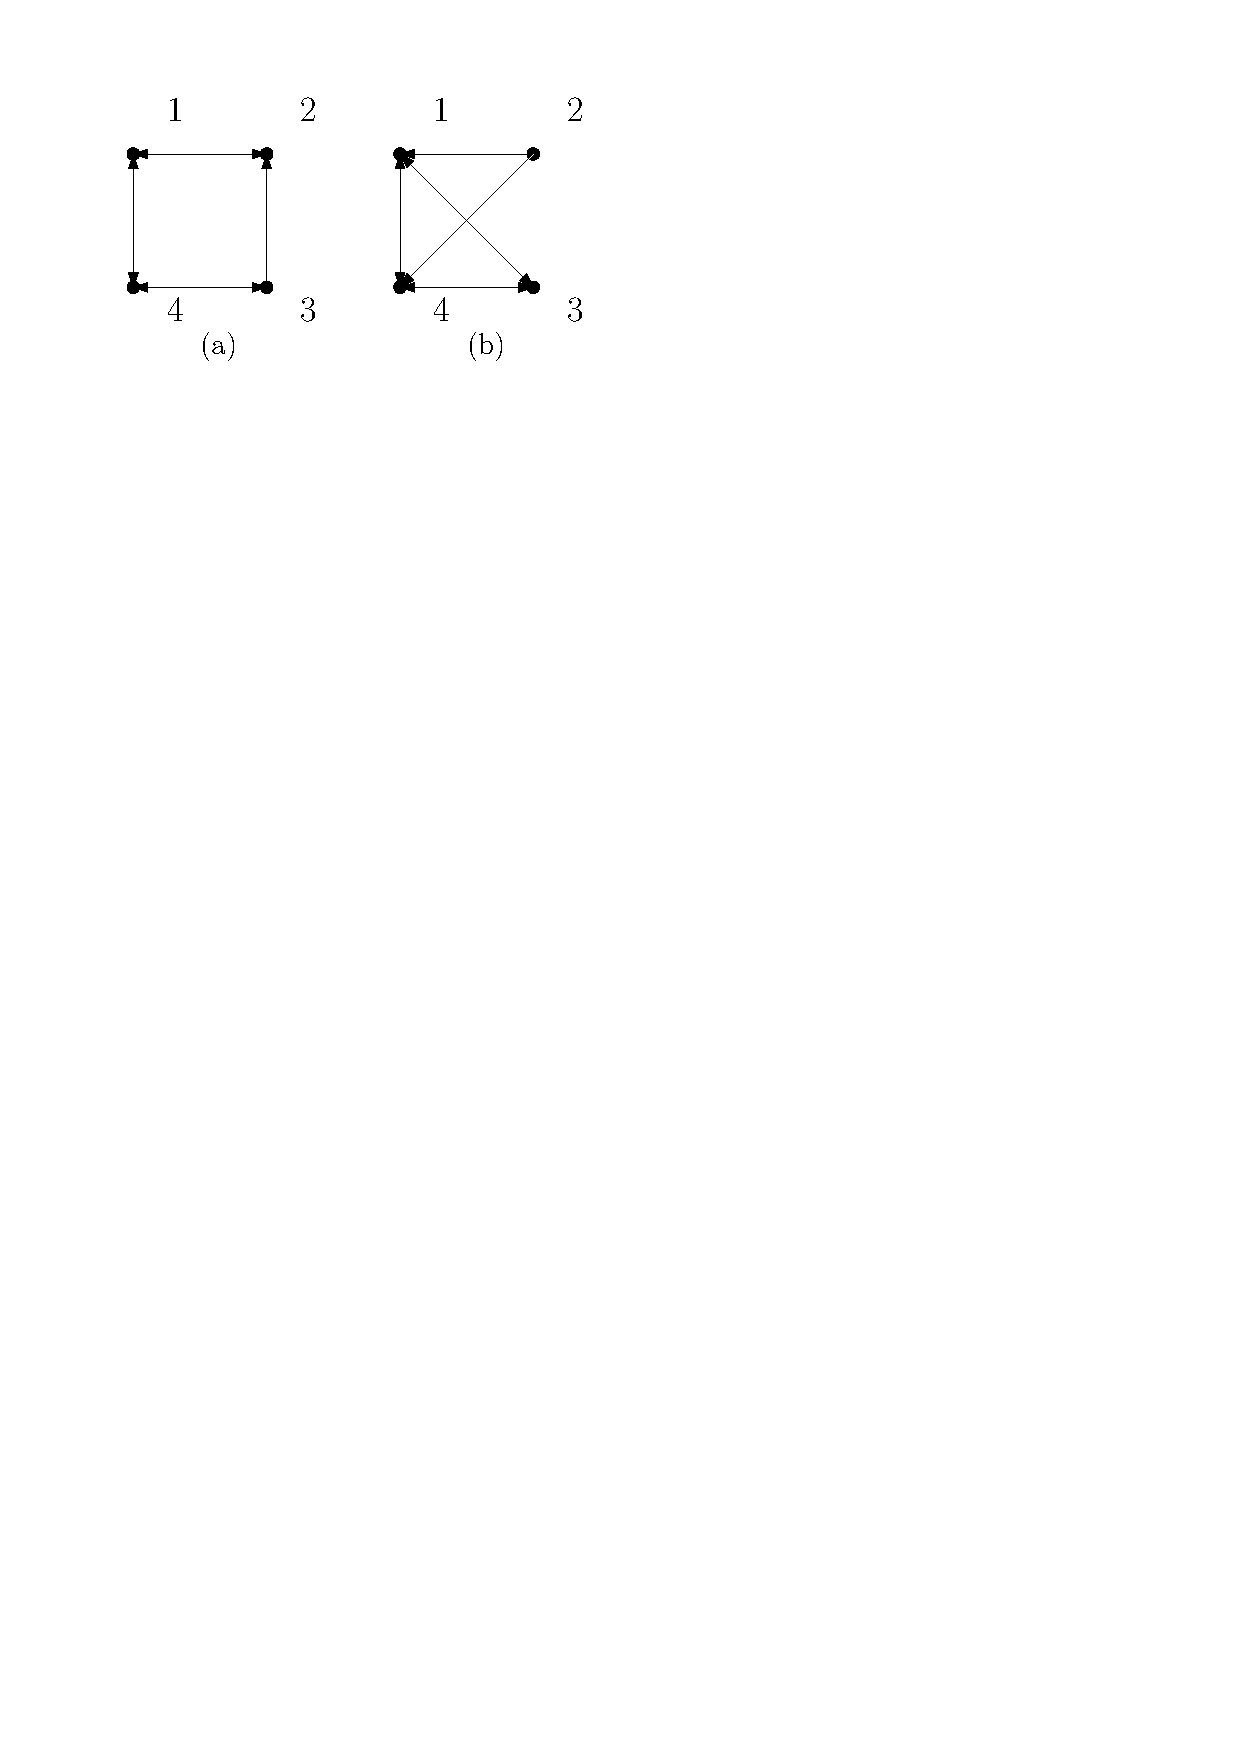
\includegraphics[scale=0.7]{2-4-20}
\end{center}
\begin{enumerate}
\item There is no clique.
\item The only clique would be the set $\{1,3,4\}$.
\end{enumerate}
\item A vertex $v$ in a tournament is called a \textbf{king} if $v$ can reach all other vertices within two steps. That is, for all vertex $u$ other than $v$, we have either $v\rightarrow u$ or $v\rightarrow w \rightarrow u$ for some $w$. So $(A+A^2)_{ij}>0$ is equivalent to that $i$ can reach $j$ within two steps. And the statement of this question also means that every tournament exists a king.

To prove this statement, we can begin by arbitrary vertex $v_1$. If $v_1$ is a king, then we've done. If $v_1$ is not a king, this means $v_1$ can not reach some vertex, say $v_2$, within two steps. Now we have that $d^+(v_2)>d^+(v_1)$ since we have $v_2\rightarrow v_1$ and that if $v_1\rightarrow w$ for some $w$ then we have $v_2\rightarrow w$ otherwise we'll have that $v_1\rightarrow w \rightarrow v_2$. Continuing this process and we can find $d^+(v_1)<d^+(v_2)<\cdots $ and terminate at some vertex $v_k$ since there are only finite vertces. And so $v_k$ would be a king.
\item We have $G=\mathcal{G}(A)$ is a tournament drawn below. And every vertex in this tournament could be a king.
\begin{center}
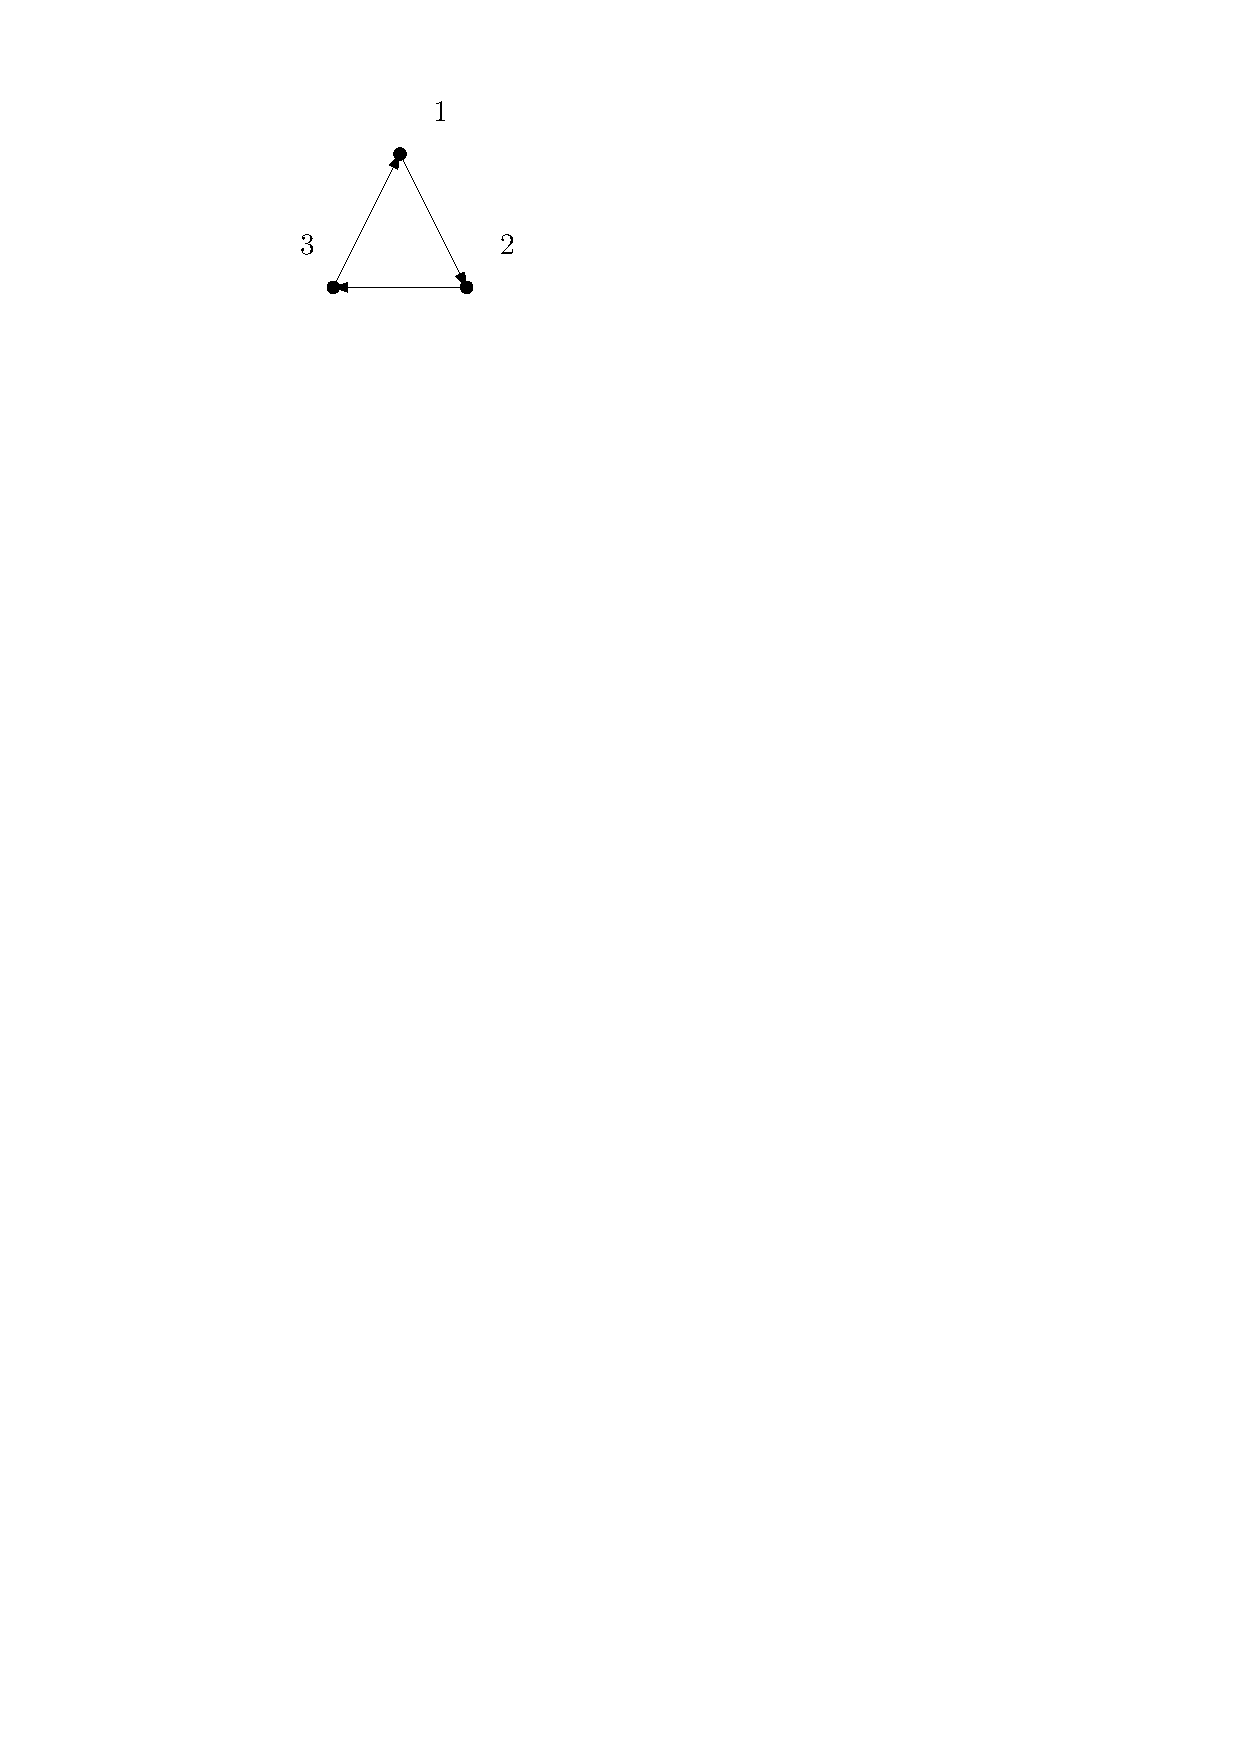
\includegraphics[scale=0.7]{2-4-22}
\end{center}
\item The number of nonzero entries would be the number of the edges in a tournament. So it would be $n(n-1)/2$.
\end{enumerate}
\section{Invertibility and Isomorphisms}
\begin{enumerate}
\item \begin{enumerate}
\item No. It should be $([T]_{\alpha }^{\beta })^{-1}=[T^{-1}]_{\beta }^{\alpha }$.
\item Yes. See Appendix B.
\item No. $L_A$ can only map $\mathbb{F}^n$ to $\mathbb{F}^m$.
\item No. It isomorphic to $\mathbb{F}^5$.
\item Yes. This is because $P_n(\mathbb{F})\cong \mathbb{F}^n$.
\item No. We have that $\left(\begin{array}{ccc}1&0&0\\0&1&0\end{array}\right) \left(\begin{array}{cc}1&0\\0&1\\0&0\end{array}\right) =I$ but $A$ and $B$ are not invertible since they are not square.
\item Yes. Since we have both $A$ and $(A^{-1})^{-1}$ are the inverse of $A^{-1}$, by the uniqueness of inverse we can conclude that they are the same.
\item Yes. We have that $L_{A^{-1}}$ would be the inverse of $L_A$.
\item Yes. This is the definition.
\end{enumerate}
\item \begin{enumerate}
\item No. They have different dimension $2$ and $3$.
\item No. They have different dimension $2$ and $3$.
\item Yes. $T^{-1}(a_1,a_2,a_3)=(-\frac{4}{3}a_2+\frac{1}{3}a_3,a_2,-\frac{1}{2}a_1-2a_2+\frac{1}{2}a_3)$.
\item No. They have different dimension $4$ and $3$.
\item No. They have different dimension $4$ and $3$.
\item Yes. $T^{-1}\left(\begin{array}{cc}a&b\\c&d \end{array}\right)=\left(\begin{array}{cc}b&a-b\\c&d-c \end{array}\right) $.
\end{enumerate}
\item \begin{enumerate}
\item No. They have different dimension $3$ and $4$.
\item Yes. They have the same dimension $4$.
\item Yes. They have the same dimension $4$.
\item No. They have different dimension $3$ and $4$.
\end{enumerate}
\item This is because that $(B^{-1}A^{-1})(AB)=(AB)(B^{-1}A^{-1})=I$.
\item This is because that $(A^{-1})^tA^t=(AA^{-1})^t=I$ and $A^t(A^{-1})^t=(A^{-1}A)^t=I$.
\item If $A$ is invertible, then $A^{-1}$ exists. So we have $B=A^{-1}AB=A^{-1}O=O$/
\item \begin{enumerate}
\item With the result of the previous exercise, if $A$ is invertible we have that $A=O$. But $O$ is not invertible. So this is a contradiction.
\item No. If $A$ is invertible then $B=O$ by the previous exercise.
\end{enumerate}
\item For Corollary 1 we may just pick $W=V$ and $\alpha =\beta $. For Corollary 2 we may just pick $V=\mathbb{F}^n$ and use Corollary 1.
\item If $AB$ is invertible then $L_{AB}$ is invertible. So $L_AL_B=L_{AB}$ is surjective and injective. And thus $L_A$ is surjective and $L_B$ injective by Exercise 2.3.12. But since their domain and codomain has the same dimension, actually they are both invertible, so are $A$ and $B$.
\item \begin{enumerate}
\item Since $AB=I_n$ is invertible, we have $A$ and $B$ is invertible by the previous exercise.
\item We have that $AB=I_n$ and $A$ is invertible. So we can conclude that \[A^{-1}=A^{-1}I_n=A^{-1}AB=B.\]
item Let $T$ is a mapping from $V$ to $W$ and $U$ is a mapping from $W$ to $V$ with dim$W=$dim$V$. If $TU$ be the identity mapping, then both $T$ and $U$ are invertible. Furthermore $T^{-1}=U$.

To prove this we may pick bases $\alpha $ of $V$ and $\beta $ of $W$ and set $A=[T]_{\alpha }^{\beta }$ and $B=[U]_{\beta }^{\alpha }$. Now apply the above arguments we have that $A$ and $B$ is invertible, so are $T$ and $U$ by Theorem 2.18.
\end{enumerate}
\item If $T(f)=0$ then we have that $f(1)=f(2)=f(3)=f(4)=0$, then we have that $f$ is zero function since it has degree at most $3$ and it's impossible to have four zeroes if $f$ is nonzero.
\item We can check $\phi _{\beta }$ is linear first. For $x=\sum_{i=1}^n{a_iv_i}$ and $y=\sum_{i=1}^n{b_iv_i}$, where \[\beta=\{v_1,v_2,\ldots ,v_n\}\] we have that 
\[\phi_{\beta }(x+cy)=\left(\begin{array}{c}a_1+cb_1\\a_2+cb_2\\\vdots \\a_n+cb_n\end{array}\right)=\left(\begin{array}{c}a_1\\a_2\\\vdots \\a_n\end{array}\right)+c\left(\begin{array}{c}b_1\\b_2\\\vdots \\b_n\end{array}\right)=\phi_{\beta}(x)+c\phi_{\beta}(y).\]
And we can check whether it is injective and surjective. If $\phi_{\beta}(x)=\left(\begin{array}{c}0\\0\\\vdots \\0\end{array}\right)$ then this means $x=\sum_{i=1}^n{0v_i}=0$. And for every $\left(\begin{array}{c}a_1\\a_2\\\vdots \\a_n\end{array}\right)+c$ in $\mathbb{F}^n$, we have that $x=\sum_{i=1}^n{a_iv_i}$ will be associated to it.
\item First we have that $V$ is isomorphic to $V$ by identity mapping. If $V$ is isomorphic to $W$ by mapping $T$, then $T^{-1}$ exist by the definition of isomorphic and $W$ is isomorphic to $V$ by $T^{-1}$. If $V$ is isomorphic to $W$ by mapping $T$ and $W$ is isomorphic to $X$ by mapping $U$, then $V$ is isomorphic to $X$ by mapping $UT$.
\item Let 
\[\beta =\{\left(\begin{array}{cc}1&1\\0&0\end{array}\right),\left(\begin{array}{cc}0&1\\0&0\end{array}\right),\left(\begin{array}{cc}0&0\\0&1\end{array}\right)\}\] be the basis of $V$. Then we have that $\phi_{\beta}$ in Theorem 2.21 would be the isomorphism.
\item We have that $T$ is isomorphism if and only if that $T$ is injective and surjective. And we also have that the later statement is equivalent to $T(\beta )$ is a baiss for $W$ by Exercise 2.1.14(c).
\item We can check that $\Phi$ is linear since 
\[\Phi(A+cD)=B^{-1}(A+cD)B=B^{-1}(AB+cDB)\]
\[=B^{-1}AB+cB^{-1}DB=\Phi(A)+c\Phi(D).\]
And it's injective since if $\Phi(A)=B^{-1}AB=O$ then we have $A=BOB^{-1}=O$. It's also be surjective since for each $D$ we have that $\Phi(BDB^{-1})=D$.
\item \begin{enumerate}
\item If $y_1,y_2\in T(V_0)$ and $y_1=T(x_1)$, $y_2=T(x_2)$, we have that $y_1+y_2=T(x_1+x_2)\in T(V_0)$ and $cy_1=T(cx_1)=T(V_0)$. Finally since $V_0$ is a subspace and so $0=T(0)\in T(V_0)$, $T(V_0)$ is a subspace of $W$.
\item We can consider a mapping $T'$ from $V_0$ to $T(V_0)$ by $T'(x)=T(x)$ for all $x\in V_0$. It's natural that $T'$ is surjective. And it's also injective since $T$ is injective. So by Dimension Theorem we have that 
\[\mathrm{dim}(V_0)=\mathrm{dim}(N(T'))+\mathrm{dim}(R(T'))=\mathrm{dim}(T(V_0)).\]
\end{enumerate}
\item With the same notation we have that 
\[L_A\phi_{\beta}(p(x))=\left(\begin{array}{cccc}0&1&0&0\\0&0&2&0\\0&0&0&3\end{array}\right)\left(\begin{array}{c}1\\1\\2\\1\end{array}\right)=\left(\begin{array}{c}1\\4\\3\end{array}\right)\]
and 
\[\phi_{\gamma}T(p(x))=\phi_{\gamma}(1+4x+3x^2)=\left(\begin{array}{c}1\\4\\3\end{array}\right).\]
So they are the same.
\item \begin{enumerate}
\item It would be 
\[\left(\begin{array}{cccc}1&0&0&0\\0&0&1&0\\0&1&0&0\\0&0&0&1\end{array}\right).\]
\item We may check that 
\[L_A\phi_{\beta}\left(\begin{array}{cc}1&2\\3&4\end{array}\right)=\left(\begin{array}{cccc}1&0&0&0\\0&0&1&0\\0&1&0&0\\0&0&0&1\end{array}\right)\left(\begin{array}{c}1\\2\\3\\4\end{array}\right)=\left(\begin{array}{c}1\\3\\2\\4\end{array}\right)\]
and 
\[\phi_{\beta}T\left(\begin{array}{cc}1&2\\3&4\end{array}\right)=\phi_{\beta}\left(\begin{array}{cc}1&3\\2&4\end{array}\right)=\left(\begin{array}{c}1\\3\\2\\4\end{array}\right).\]
So they are the same.
\end{enumerate}
\item With the notation in Figure 2.2 we can prove first that $\phi_{\gamma}(R(T))=L_A(\mathbb{F}^n)$. Since $\phi_{\beta}$ is surjective we have that 
\[L_A(\mathbb{F}^n)=L_A\phi_{\beta}(V)=\phi_{\gamma}T(V)=\phi_{\gamma}(R(T)).\]
Since $R(T)$ is a subspace of $W$ and $\phi_{\gamma}$ is an isomorphism, we have that rank$(T)=$rank$(L_A)$ by Exercise 2.4.17.

On the other hand, we may prove that $\phi_{\beta}(N(T))=N(L_A)$. If $y\in \phi_{\beta}(N(T))$, then we have that $y=\phi_{\beta}(x)$ for some $x\in N(T)$ and hence \[L_A(y)=L_A(\phi_{\beta}(x))=\phi_{\gamma}T(x)=\phi_{\gamma}(0)=0.\]
Conversely, if $y\in N(L_A)$, then we have that $L_A(y)=0$. Since $\phi_{\beta}$ is surjective, we have $y=\phi_{\beta}(x)$ for some $x\in V$. But we also have that 
\[\phi_{\gamma}(T(x))=L_A(\phi_{\beta}(x))=L_A(y)=0\]
and $T(x)=0$ since $\phi_{\gamma}$ is injective. So similarly by Exercise 2.4.17 we can conclude that nullity$(T)=$nullity$(L_A)$.
\item First we prove the independence of $\{T_{ij}\}$. Suppose that $\sum_{i,j}{a_{ij}T_{ij}}=0$. We have that 
\[(\sum_{i,j}{a_{ij}T_{ij}})(v_k)=\sum_{i}{a_{ij}T_{ik}(v_k)}=\sum_{i}{a_{ik}w_i}=0.\]
This means $a_{ik}=0$ for all proper $i$ since $\{w_i\}$ is a basis. And since $k$ is arbitrary we have that $a_{ik}=0$ for all $i$ and $k$.

Second we prove that $[T_{ij}]_{\beta}^{\gamma}=M^{ij}$. But this is the instant result of 
\[T_{ij}(v_j)=w_j\]
and 
\[T_{ij}(v_k)=0\]
for $k\neq j$. Finally we can observe that $\Phi(\beta )=\gamma $ is a basis for $M_{m\times n}(\mathbb{F})$ and so $\Phi $ is a isomorphism by Exercise 2.4.15.
\item It's linear since 
\[T(f+cg)=((f+cg)(c_0),(f+cg)(c_1),\ldots (f+cg)(c_n))\]
\[=(f(c_0)+cg(c_0),f(c_1)+cg(c_1),\ldots f(c_n)+cg(c_n))=T(f)+cT(g).\]
Since $T(f)=0$ means $f$ has $n+1$ zeroes, we know that $f$ must be zero function( This fact can be proven by Lagrange polynomial basis for $P_n(\mathbb{F})$.). So $T$ is injective and it will also be surjective since domain and codomain have same finite dimension.
\item The transformation is linear since 
\[T(\sigma +c\tau )=\sum_{i=0}^m{(\sigma +c\tau )(i)x^i}\]
\[=\sum_{i=0}^m{\sigma (i)x^i+c\tau (i)x^i}=T(\sigma )+cT(\tau ),\]
where $m$ is a integer large enough such that $\sigma (k)=\tau (k)=0$ for all $k>m$.
It would be injective by following argument. Since $T(\sigma )=\sum_{i=0}^n{\sigma (i)x^i}=0$ means $\sigma (i)=0$ for all integer $i\leq n$, with the help of the choice of $n$ we can conclude that $\sigma =0$. On the other hand, it would also be surjective since for all polynomial $\sum_{i=0}^n{a_ix^i}$ we may let $\sigma (i)=a_i$ and thus $T$ will map $\sigma $ to the polynomial.
\item \begin{enumerate}
\item If $v+N(T)=v'+N(T)$, we have that $v-v'\in N(T)$ and thus $T(v)-T(v')=T(v-v')=0$.
\item We have that 
\[\bar{T}((v+N(T))+c(u+N(T)))=\bar{T}((v+cu)+N(T))\]
\[=T(v+cu)=T(v)+cT(u).\]
\item Since $T$ is surjective, for all $y\in Z$ we have $y=T(x)$ for some $x$ and hence $y=\bar{T}(x+N(T))$. This means $\bar{T}$ is also surjective. On the other hand, if $\bar{T}(x+N(T))=T(x)=0$ then we have that $x\in N(T)$ and hence $x+N(T)=0+N(T)$. So $\bar{T}$ is injective. With these argument $\bar{T}$ is an isomorphism.
\item For arbitrary $x\in V$, we have 
\[\bar{T}_{\eta }(x)=\bar{T}(x+N(T))=T(x).\]
\end{enumerate}
\item The transformation $\Psi $ would be linear since 
\[\Psi(f+cg)=\sum_{(f+cg)(s)\neq 0}{(f+cg)(s)s}=\sum_{(f+cg)(s)\neq 0}{f(s)s+cg(s)s}\]
\[=\sum_{(f\enspace \mathrm{or} \enspace cg)(s)\neq 0}{f(s)s+cg(s)s}=\sum_{(f\enspace \mathrm{or} \enspace cg)(s)\neq 0}{f(s)}+c\sum_{(f\enspace \mathrm{or} \enspace cg)(s)\neq 0}{g(s)s}\]
\[=\Psi(f)+c\Psi(g).\]
It will be injective by following arguments. If $\Psi(f)=\sum_{f(s)\neq 0}{f(s)s}=0$ then we have that $f(s)=0$ on those $s$ such that $f(s)\neq 0$ since $\{s:f(s)\neq 0\}$ is finite subset of basis. But this can only be possible when $f=0$. On the other hand, we have for all element $x\in V$ we can write $x=\sum_{i}{a_is_i}$ for some finite subset $\{s_i\}$ of $S$. Thus we may pick a function $f$ sucht that $f(s_i)=a_i$ for all $i$ and vanish outside. Thus $\Psi $ will map $f$ to $x$. So $\Psi $ is surjective. And thus it's an isomorphism.
\end{enumerate}
\section{The Change of Coordinate Matrix}
\begin{enumerate}
\item \begin{enumerate}
\item No. It should be $[x_j']_{\beta}$.
\item Yes. This is Theorem 2.22.
\item Yes. This is Theorem 2.23.
\item No. It should be $B=Q^{-1}AQ$.
\item Yes. This is the instant result of the definition of similar and Theorem 2.23.
\end{enumerate}
\item For these problem, just calculate $[I]_{\beta'}^{\beta}$.\begin{enumerate}
\item $\left(\begin{array}{cc}a_1&b_1\\a_2&b_2\end{array}\right).$
\item $\left(\begin{array}{cc}4&1\\2&3\end{array}\right).$
\item $\left(\begin{array}{cc}3&-1\\5&-2\end{array}\right).$
\item $\left(\begin{array}{cc}2&-1\\5&-4\end{array}\right).$
\end{enumerate}
\item \begin{enumerate}
\item $\left(\begin{array}{ccc}a_2&b_2&c_2\\a_1&b_1&c_1\\a_0&b_0&c_0\end{array}\right).$
\item $\left(\begin{array}{ccc}a_0&b_0&c_0\\a_1&b_1&c_1\\a_2&b_2&c_2\end{array}\right).$
\item $\left(\begin{array}{ccc}0&-1&0\\1&0&0\\-3&2&1\end{array}\right).$
\item $\left(\begin{array}{ccc}2&1&1\\3&-2&1\\-1&3&1\end{array}\right).$
\item $\left(\begin{array}{ccc}5&-6&3\\0&4&-1\\3&-1&2\end{array}\right).$
\item $\left(\begin{array}{ccc}-2&1&2\\3&4&1\\-1&5&2\end{array}\right).$
\end{enumerate}
\item We have that 
\[[T]_{\beta}=\left(\begin{array}{cc}2&1\\1&-3\end{array}\right)\]
and
\[[T]_{\beta'}=[I]_{\beta}^{\beta'}[[T]_{\beta}[I]_{\beta'}^{\beta}\]
\[=\left(\begin{array}{cc}2&-1\\-1&1\end{array}\right)\left(\begin{array}{cc}2&1\\1&-3\end{array}\right)\left(\begin{array}{cc}1&1\\1&2\end{array}\right)\]
\[=\left(\begin{array}{cc}8&13\\-5&-9\end{array}\right).\]
\item We have that 
\[[T]_{\beta}=\left(\begin{array}{cc}0&0\\1&0\end{array}\right)\]
and
\[[T]_{\beta'}=[I]_{\beta}^{\beta'}[T]_{\beta}[I]_{\beta'}^{\beta}\]
\[=\left(\begin{array}{cc}\frac{1}{2}&\frac{1}{2}\\\frac{1}{2}&-\frac{1}{2}\end{array}\right)\left(\begin{array}{cc}0&1\\0&0\end{array}\right)\left(\begin{array}{cc}1&1\\1&-1\end{array}\right)\]
\[=\left(\begin{array}{cc}\frac{1}{2}&-\frac{1}{2}\\\frac{1}{2}&-\frac{1}{2}\end{array}\right).\]
\item Let $\alpha $ be the standard basis (of $\mathbb{F}^2$ or $\mathbb{F}^3$). We have that $A=[L_A]_{\alpha}$ and hence $[L_A]_{\beta}=[I]_{\alpha}^{\beta}[L_A]_{\alpha}[I]_{\beta}^{\alpha}$. So now we can calculate $[L_A]_{\beta}$ and $Q=[I]_{\beta}^{\alpha}$ and $Q^{-1}=[I]_{\alpha}^{\beta}$.
\begin{enumerate}
\item $[L_A]_{\beta}=\left(\begin{array}{cc}6&11\\-2&-4\end{array}\right)$ and $Q=\left(\begin{array}{cc}1&1\\1&2\end{array}\right)$.
\item $[L_A]_{\beta}=\left(\begin{array}{cc}3&0\\0&-1\end{array}\right)$ and $Q=\left(\begin{array}{cc}1&1\\1&-1\end{array}\right)$.
\item $[L_A]_{\beta}=\left(\begin{array}{ccc}2&2&2\\-2&-3&-4\\1&1&2\end{array}\right)$ and $Q=\left(\begin{array}{ccc}1&1&1\\1&0&1\\1&1&2\end{array}\right)$.
\item $[L_A]_{\beta}=\left(\begin{array}{ccc}6&0&0\\0&12&0\\0&0&18\end{array}\right)$ and $Q=\left(\begin{array}{ccc}1&1&1\\1&-1&1\\-2&0&1\end{array}\right)$.
\end{enumerate}
\item We may let $\beta $ be the standard basis and $\alpha=\{(1,m),(-m,1)\}$ be another basis for $\mathbb{R}^2$.
\begin{enumerate}
\item We have that $[T]_{\alpha}=\left(\begin{array}{cc}1&0\\0&-1\end{array}\right)$ and $Q^{-1}=[I]_{\alpha}^{\beta}=\left(\begin{array}{cc}1&m\\-m&1\end{array}\right)$. We also can calculate that $Q=[I]_{\beta}^{\alpha}=\left(\begin{array}{cc}\frac{1}{m^2+1}&\frac{m}{m^2+1}\\-\frac{m}{m^2+1}&\frac{1}{m^2+1}\end{array}\right)$. So finally we get 
\[[T]_{\beta}=Q^{-1}[T]_{\alpha}Q=\left(\begin{array}{cc}\frac{1-m^2}{m^2+1}&\frac{2m}{m^2+1}\\\frac{2m}{m^2+1}&\frac{m^2-1}{m^2+1}\end{array}\right).\]
That is, $T(x,y)=(\frac{x+2ym-xm^2}{m^2+1},\frac{-y+2xm+ym^2}{m^2+1})$.
\item Similarly we have that $[T]_{\alpha}=\left(\begin{array}{cc}1&0\\0&0\end{array}\right)$. And with the same $Q$ and $Q^{-1}$ we get 
\[[T]_{\beta}=Q^{-1}[T]_{\alpha}Q=\left(\begin{array}{cc}\frac{1}{m^2+1}&\frac{m}{m^2+1}\\\frac{m}{m^2+1}&\frac{m^2}{m^2+1}\end{array}\right).\]
That is, $T(x,y)=(\frac{x+ym}{m^2+1},\frac{xm+ym^2}{m^2+1})$.
\end{enumerate}
\item This is similar to the proof of Theorem 2.23 since 
\[[T]_{\beta'}^{\gamma'}=[I_W]_{\gamma}^{\gamma'}[T]_{\beta}^{\gamma}[I_V]_{\beta'}^{\beta}=P^{-1}[T]_{\beta}^{\gamma}Q.\]
\item We may denote that $A$ is similar to $B$ by $A\sim B$. First we have $A=I^{-1}AI$ and hence $A\sim A$. Second, if $A\sim B$ we have $A=Q^{-1}BQ$ and $B=(Q^{-1})^{-1}AQ^{-1}$ and hence $B\sim A$. Finally, if $A\sim B$ and $B\sim C$ then we have $A=P^{-1}BP$ and $B=Q^{-1}CQ$. And this means $A=(QP)^{-1}C(QP)$ and hence $A\sim C$. So it's a equivalence relation.
\item If $A$ and $B$ are similar, we have $A=Q^{-1}BQ$ for some invertible matrix $Q$. So we have 
\[\mathrm{tr}(A)=\mathrm{tr}(Q^{-1}BQ)=\mathrm{tr}(QQ^{-1}B)=\mathrm{tr}(B)\]
by  Exercise 2.3.13.
\item \begin{enumerate}
\item This is because 
\[RQ=[I]_{\beta}^{\gamma}[I]_{\alpha}^{\beta}=[I]_{\alpha}^{\gamma}.\]
\item This is because 
\[Q^{-1}=([I]_{\alpha}^{\beta})^{-1}=[I^{-1}]_{\beta}^{\alpha}=[I]_{\beta}^{\alpha}.\]
\end{enumerate}
\item This is the instant result that $A=[L_A]_{\beta}$ and $Q$ defined in the Corollary is actually $[I]_{\gamma}^{\beta}$.
\item Since $Q$ is invertible, we have that $L_Q$ is invertible. We try to check $\beta'$ is an independent set and hence a basis since $V$ has dimension $n$. Suppose that $\sum_{j=1}^n{a_jx_j'}=0$. And it means that 
\[\sum_{j=1}^n{a_j\sum_{i=1}^n{Q_{ij}x_i}}=\sum_{i=1}^n{(\sum_{j=1}^n{a_jQ_{ij}})x_i}=0.\]
Since $\beta $ is a basis, we have that $\sum_{j=1}^n{a_jQ_{ij}}=0$ for all $i$. Actually this is a system of linear equations and can be written as 
\[\left(\begin{array}{cccc}a_1&a_2&\ldots &a_n\end{array}\right)\left(\begin{array}{cccc}Q_{11}&Q_{12}&\cdots &Q_{1n}\\Q_{21}&Q_{22}&\cdots &Q_{2n}\\\vdots &\vdots &\ddots &\vdots \\Q_{n1}&Q_{n2}&\cdots &Q_{nn}\end{array}\right)=vQ=0,\]
where $v=\left(\begin{array}{cccc}a_1&a_2&\ldots &a_n\end{array}\right)$.
But since $Q$ is invertible and so $Q^{-1}$ exist, we can deduce that $v=vQQ^{-1}=0Q^{-1}=0$. So we know that $\beta $ is a basis. And it's easy to see that $Q=[I]_{\beta}^{\beta}$ is the change of coordinate matrix changing $\beta'$-coordinates into $\beta$-coordinates.
\item Let $V=\mathbb{F}^n$, $W=\mathbb{F}^m$, $T=L_A$, $\beta $, and $\gamma $ be the notation defined in the Hint. Let $\beta'$ and $\gamma'$ be the set of column vectors of $Q$ and $P$ respectly. By Exercise 2.5.13 we have that $\beta'$ and $\gamma'$ are bases and $Q=[I]_{\beta'}^{\beta}$, $P=[I]_{\gamma'}^{\gamma}$. Since we have that $[T]_{\beta'}^{\gamma'}=[I]_{\gamma}^{\gamma'}[T]_{\beta}^{\gamma}[I]_{\beta'}^{\beta}$, we have that $B=P^{-1}AQ$.
\end{enumerate}

\section{Dual Spaces}
\begin{enumerate}
\item \begin{enumerate}
\item No. Every linear functional is a linear transformation.
\item Yes. It's domain and codomain has dimension $1$.
\item Yes. They have the same dimension.
\item Yes. It's isomorphic to the dual space of its dual space. But if the ``is'' here in this question means ``equal'', then it may not be true since dual space must has that its codomain should be $\mathbb{F}$.
\item No. For an easy example we may let $T$ be the linear transformation such that $T(x_i)=2f_i$, where $\beta\{x_1,x_2,\ldots ,x_n\}$ is the basis for $V$ and $\beta^*\{f_1,f_2,\ldots ,f_n\}$ is the corresponding dual basis for $V^*$.
\item Yes.
\item Yes. They have the same dimension.
\item No. Codomain of a linear functional should be the field.
\end{enumerate}
\item In these question we should check whether it's linear and whether its domain and codomain are $V$ and $F$ respectly. \begin{enumerate}
\item Yes. We may check that \[f(p(x)+cq(x))=2p'(0)+2cp'(0)+p''(1)+cq''(1)\]
\[2p'(0)+p''(1)+c(2p'(0)+q''(1))=f(p(x))+cf(q(x)).\]
\item No. It's codomain should be the field.
\item Yes. We may check that \[\mathrm{tr}(A+cB)=\sum_{i=1}^n{(A+cB)_{ii}}\]
\[=\sum_{i=1}^n{A_{ii}+cB_{ii}}=\mathrm{tr}(A)+c\mathrm{tr}(B).\]
\item No. It's not linear.
\item Yes. We may check that \[f(p(x)+cq(x))=\int_0^1(p(t)+cq(t))dt\]
\[=\int_0^1p(t)dt+c\int_0^1q(t)dt=f(p(x))+cf(q(x)).\]
\item Yes. We may check that \[f(A+cB)=(A+cB)_{11}=A_{11}+cB_{11}=f(A)+cf(B).\]
\end{enumerate}
\item \begin{enumerate}
\item We may find out that for all vector $(x,y,z)\in \mathbb{R}^3$ we can express it as 
\[(x,y,z)=(x-\frac{y}{2})(1,0,1)+\frac{y}{2}(1,2,1)+(z-x)(0,0,1).\]
So we can write 
\[\left\{\begin{array}{l}f_1(x,y,z)=x-\frac{y}{2};\\f_2(x,y,z)=\frac{y}{2};\\f_3(x,y,z)=z-x.\end{array}\right.\]
\item This is much easier and we have that 
\[\left\{\begin{array}{l}f_1(a_0+a_1x+a_2x^2)=a_0;\\f_2(a_0+a_1x+a_2x^2)=a_1;\\f_3(a_0+a_1x+a_2x^2)=a_2.\end{array}\right.\]
\end{enumerate}
\item We may returen the representation such that 
\[(x,y,z)=(x-2y)(\frac{2}{5},-\frac{3}{10},-\frac{1}{10})+(x+y+z)(\frac{3}{5},\frac{3}{10},\frac{1}{10})+(y-3z)(\frac{1}{5},\frac{1}{10},-\frac{3}{10}).\]
We may check that the set $\{(\frac{2}{5},-\frac{3}{10},-\frac{1}{10}),(\frac{3}{5},\frac{3}{10},\frac{1}{10}),(\frac{1}{5},\frac{1}{10},-\frac{3}{10})\}$ is a basis and hence the desired set. By Theorem 2.24 $\{f_1,f_2,f_3\}$ is a basis for $V^*$.
\item Assume that $p(t)=a+bx$. We have $\int_0^1{(a+bt)}dt=a+\frac{b}{2}$ and $\int_0^2{(a+bt)}dt=2a+2b$. So we may returen the representation such that 
\[a+bx=(a+\frac{b}{2})(2-2x)+(2a+2b)(-\frac{1}{2}+x).\]
We may check that the set $\{2-2x,-\frac{1}{2}+x\}$ is a basis and hence the desired set. By Theorem 2.24 $\{f_1,f_2,f_3\}$ is a basis for $V^*$.
\item \begin{enumerate}
\item Calculate directly that 
\[T^t(f)(x,y)=fT(x,y)=f(3x+2y,x)=7x+4y.\]
\item Since $\beta=\{(1,0),(0,1)\}$ and $(x,y)=x(1,0)+y(0,1)$, we have that $f_1(x,y)=x$ and $f_2(x,y)=y$. So we can find out that 
\[T^t(f_1)(x,y)=f_1T(x,y)=f_1(3x+2y,x)=3x+2y=3f_1(x,y)+2f_2(x,y);\]
\[T^t(f_2)(x,y)=f_2T(x,y)=f_2(3x+2y,x)=x=1f_1(x,y)+0f_2(x,y).\]
And we have the matrix $[T^t]_{\beta^*}=\left(\begin{array}{cc}3&1\\2&0\end{array}\right).$
\item Since $T(x,y)=(3x+2y,x)$, we can calculate that 
\[[T]_{\beta}=\left(\begin{array}{cc}3&2\\1&0\end{array}\right)\]
and 
\[([T]_{\beta})^t=\left(\begin{array}{cc}3&1\\2&0\end{array}\right).\]
So we have that $[T^t]_{\beta^*}=([T]_{\beta})^t$.
\end{enumerate}
\item \begin{enumerate}
\item Calculate directly that 
\[T^t(f)(a+bx)=fT(a+bx)=f(-a-2b,a+b)=-3a-4b.\]
\item Since $\beta=\{1,x\}$ and $a+bx=a\times 1+b\times x$, we have that $f_1(a+bx)=a$ and $f_2(a+bx)=b$. And since $\gamma=\{(1,0),(0,1)\}$ and $(a,b)=a(1,0)+b(0,1)$, we have that $g_1(a,b)=a$ and $g_2(a,b)=b$. So we can find out that 
\[T^t(g_1)(a+bx)=g_1T(a+bx)=g_1(-a-2b,a+b)=-a-2b\]
\[=-1\times g_1(a,b)+(-2)\times g_2(a,b);\]
\[T^t(g_2)(a+bx)=g_2T(a+bx)=g_2(-a-2b,a+b)=a+b\]
\[=1\times g_1(a,b)+1\times g_2(a,b).\]
And we have the matrix $[T^t]_{\gamma^*}^{\beta^*}=\left(\begin{array}{cc}-1&1\\-2&1\end{array}\right).$
\item Since $T(a+bx)=(-a-2b,a+b)$, we can calculate that 
\[[T]_{\beta}^{\gamma}=\left(\begin{array}{cc}-1&-2\\1&1\end{array}\right)\]
and 
\[([T]_{\beta}^{\gamma})^t=\left(\begin{array}{cc}-1&1\\-2&1\end{array}\right).\]
So we have that $[T^t]_{\gamma^*}^{\beta^*}=([T]_{\beta}^{\gamma})^t$.
\end{enumerate}
\item Every plane could be written in the form $P=\{(x,y,z):ax+by+cz=0\}$ for some scalar $a$, $b$ and $c$. Consider a transformation $T(x,y,z)=ax+by+cz$. It can be shown that $T$ is an element in $(\mathbb{R}^3)^*$ and $P=N(T)$. For the case in $\mathbb{R}^2$, actually every line has the form $L=\{(x,y):ax+by=0\}$ and hence is the null space of a vector in $(\mathbb{R}^2)^*$.
\item If $T$ is linear, we can set $f_i$ be $g_iT$ as the Hint. Since it's conposition of two linear function, it's linear. So we have 
\[T(x)=(g_1(T(x)),g_2(T(x)),\ldots ,g_m(T(x)))\]
\[=(f_1(x),f_2(x),\ldots ,f_m(x)).\]

For the converse, let $\{e_i\}_{i=1,2,\ldots ,m}$ be the standard basis of $\mathbb{F}^m$. So if we have that $T(x)=\sum_{i=1}^m{f_i(x)e_i}$ with $f_i$ linear, we can define $T_i(x)=f_i(x)e_i$ and it would be a linear transformation in $\mathscr{L}(\mathbb{F}^n,\mathbb{F}^m)$. Thus we know $T$ is linear since $T$ is summation of all $T_i$.
\item \begin{enumerate}
\item Since we can check that $f_i(p(x)+cq(x))=p(c_i)+cq(c_i)=f_i(p(x))+cf_i(q(x))$, $f_i$ is linear and hence in $V^*$. And we know that $\mathrm{dim}(V^*)=\mathrm{dim}(V)=\mathrm{dim}(P_n(\mathbb{F}))=n+1$. So now it's enough to show that $\{f_0,f_1,\ldots ,f_n\}$ is independent. So assume that $\sum_{i=1}^n{a_if_i}=0$ for some $a_i$. We may define polynomials $p_i(x)=\prod_{j\neq i}{(x-c_j)}$ such that we know $p_i(c_i)\neq 0$ but $p_i(c_j)=0$ for all $j\neq i$. So now we have that 
\[\sum_{i=1}^n{a_if_i(p_1)}=a_1f_1(p_1)=0\]
implies $a_1=0$. Similarly we have $a_i=0$ for all proper $i$.
\item By the Corollary after Theorem 2.26 we have an ordered basis 
\[\beta =\{p_0,p_1,\ldots ,p_n\}\] for $V$ such that $\{f_1,f_2,\ldots ,f_n\}$ defined in the previous exercise is its dual basis. So we know that $p_i(c_j)=\delta_{ij}$. Since $\beta $ is a basis, every polynomial in $V$ is linear combination of $\beta $. If a polynomial $q$ has the property that $q(c_j)=\delta_{0j}$, we can assume that $q=\sum_{i=0}^n{a_ip_i}$. Then we have 
\[1=q(c_0)=\sum_{i=0}^n{a_ip_i(c_0)}=a_1\]
and 
\[0=q(c_j)=\sum_{i=0}^n{a_ip_i(c_j)}=a_j\]
for all $j$ other than $1$. So actually we know $q=p_0$. This means $p_0$ is unique. And similarly we know all $p_i$ is unique. Since the Lagrange polynomials,say $\{r_i\}_{i=1,2,\ldots n}$, defined in Section 1.6 satisfy the property $r_i(c_j)=\delta_{ij}$, by uniqueness we have $r_i=p_i$ for all $i$.
\item Let $\beta =\{p_0,p_1,\ldots ,p_n\}$ be those polynomials defined above. We may check that 
\[q(x)=\sum_{i=0}^n{a_ip_i(x)}\]
has the property $q(c_i)=a_i$ for all $i$, since we know that $p_i(c_j)=\delta_{ij}$. Next if $r(x)\in V$ also has the property, we may assume that 
\[r(x)=\sum_{i=0}^n{b_ip_i(x)}\]
since $\beta $ is a basis for $V$. Similarly we have that 
\[a_i=r(c_i)=\sum_{i=0}^n{b_ip_i(c_i)=b_i}.\]
So we know $r=q$ and $q$ is unique.
\item This is the instant result of 2.6.10(a) and 2.6.10(b) by setting $a_i=p(c_i)$.
\item Since there are only finite term in that summation, we have that the order of integration and summation can be changed. So we know 
\[\int_a^b{p(t)dt}=\int_a^b{(\sum_{i=0}^n{p(c_i)p_i(t)})dt}\]
\[=\sum_{i=0}^n{\int_a^b{p(c_i)p_i(t)dt}}.\]
\end{enumerate}
\item It will be more clearer that we confirm that the domain and codomain of both $\psi_2T$ and $T^{tt}\psi_2$ are $V$ and $W^{**}$ respectly first.
So for all $x\in V$ we have 
\[\psi_2T(x)=\psi(T(x))=\hat{T(x)}\in W^{**}\]
and 
\[T^{tt}\psi_1(x)=T^{tt}(\hat{x})\]
\[=(T^t)^t(\hat{x})=\hat{x}T^t\in W^{**}.\]
But to determine whether two elements $f$ and $g$ in $W^{**}$ are the same is to check whether the value of $f(h)$ and $g(h)$ are the same for all $h\in W^*$. So let $h$ be an element in $W*$. Let's check that 
\[\hat{T(x)}(h)=h(T(x))\]
and 
\[\hat{x}T^t(h)=\hat{x}(hT)=h(T(x)).\]
So we know they are the same.
\item Let $\beta =\{x_1,x_2,\ldots ,x_n\}$ be a basis for $V$. Then we know the functional $\hat{x_i}\in V^{**}$ means $\hat{x_i}(f)=f(x_i)$ for all funtional $f$ in $V^*$. On the other hand, we have the dual basis $\beta^*=\{f_1,f_2,\ldots, f_n\}$ is defined by $f_i(x_j)=\delta_{ij}$ for all $i=1,2,\ldots ,n$ and $j=1,2,\ldots ,n$ such that $f_i$ is lineaer. And we can further ferret what elements are in $\beta^{**}$. By definition of $\beta ^{**}$ we know $\beta^{**}=\{F_1,F_2,\ldots, F_n\}$ and $F_i(f_j)=\delta_{ij}$ and $F_i$ is linear. So we may check that whether $F_i=\hat{x_i}$ by 
\[\hat{x_i}(f_j)=f_j(x_i)=\delta_{ij}=F_i(f_j).\]
Since they are all linear functionals and the values of them meet at basis $\beta^*$, they are actually equal by the Corollary after Theorem 2.6.
\item \begin{enumerate}
\item We can check that $f+g$ and $cf$ are elements in $S^0$ if $f$ and $g$ are elements in $S^0$ since $(f+g)(x)=f(x)+g(x)=0$ and $(cf)(x)=cf(x)=0$. And the zero function is an element in $S^0$.
\item Let $\{v_1,v_2,\ldots ,v_k\}$ be the basis of $W$. Since $x\notin W$ we know that $\{v_1,v_2,\ldots ,v_{k+1}=x\}$ is an independent set and hence we can extend it to a basis $\{v_1,v_2,\ldots ,v_n\}$ for $V$. So we can define a linear transformation $T$ such that $f(v_i)=\delta_{i(k+1)}$. And thus $f$ is the desired functional.
\item Let $W$ be the subspace span$(S)$. We first prove that $W^0=S^0$. Since every function who is zero at $W$ must be a function who is zero at $S$. we know $W^0\subset S^0$. On the other hand, if a linear function has the property that $f(x)=0$ for all $x\in S$, we can deduce that $f(y)=0$ for all $y\in W=$span$(S)$. Hence we know that $W^0\supset S^0$ and $W^0=S^0$. Since $(W^0)^0=(S^0)^0$ and span$(\psi(S))=\psi(W)$ by the fact $\psi$ is an isomorphism, we can just prove that $(W^0)^0=\psi(W)$.

Next, by Theorem 2.26 we may assume every element in $(W^0)^0\subset V^{**}$ has the form $\hat{x}$ for some $x$. Let $\hat{x}$ is an element in $(W^0)^0$. We have that $\hat{x}(f)=f(x)=0$ if $f\in W^0$. Now if $x$ is not an element in $W$, by the previous exercise there exist some functional $f\in W^0$ such that $f(x)\neq 0$. But this is a contradiction. So we know that $\hat{x}$ is an element in $\psi(W)$ and $(W^0)^0\subset \psi(W)$.

For the converse, we may assume that $\hat{x}$ is an element in $\psi(W)$. Thus for all $f\in W^0$ we have that $\hat{x}(f)=f(x)=0$ since $x$ is an element in $W$. So we know that $(W^0)^0\supset \psi(W)$ and get the desired conclusion.
\item It's natural that if $W_1=W_2$ then we have $W_1^0=W_2^0$. For the converse, if $W_1^0=W_2^0$ then we have 
\[\psi(W_1)=(W_1^0)^0=(W_2^0)^0=\psi(W_2)\]
and hence 
\[W_1=\psi^{-1}\psi(W_1)=\psi^{-1}\psi(W_2)=W_2\]
by the fact that $\psi$ is an isomorphism.
\item If $f$ is an element in $(W_1+W_2)^0$, we have that $f(w_1+w_2)=0$ for all $w_1\in W_1$ and $w_2\in W_2$. So we know that $f(w_1+0)=0$ and $f(0+w_2)=0$ for all proper $w_1$ and $w_2$. This means $f$ is an element in $W_1^0\cap W_2^0$. For the converse, if $f$ is an element in $W_1^0\cap W_2^0$, we have that $f(w_1+w_2)=f(w_1)+f(w_2)=0$ for all $w_1\in W_1$ and $w_2\in W_2$. Hence we have that $f$ is an element in $(W_1+W_2)^0$.
\end{enumerate}
\item We use the notation in the Hint. To prove that $\alpha=\{f_{k+1},f_{k+2},\ldots ,f_n\}$ is a basis for $W^0$, we should only need to prove that span$(\alpha )=W^0$ since by $\alpha \subset \beta^*$ we already know that $\alpha $ is an independent set. Since $W^0\subset V^*$, every element $f\in W^0$ we could write $f=\sum_{i=1}^n{a_if_i}$. Next since for $1\leq i \leq k$ $x_i$ is an element in $W$, we know that 
\[0=f(x_i)=\sum_{i=1}^n{a_if_i(x_i)}=a_i.\] 
So actually we have $f=\sum_{i=k+1}^n{a_if_i}$ is an element in span$(\alpha )$. And finally we get the conclusion by 
\[\mathrm{dim}(W)+\mathrm{dim}(W_0)=k+(n-k)=n=\mathrm{dim}(V).\]
\item If $T^t(f)=fT=0$, this means $f(y)=0$ for all $y\in R(T)$ and hence $f\in (R(T))^0$. If $f\in (R(T))^0$, this means $f(y)=0$ for all $y\in R(T)$ and hence $T^t(f)(x)=f(T(x))=0$ for all $x$. This means $f$ is an element in $N(T^t)$.
\item We have that 
\[\mathrm{rank}(L_A)=\mathrm{dim}(R(L_A))=m-\mathrm{dim}(R(L_A)^0)=m-\mathrm{dim}(N((L_A)^t))\]
\[=\mathrm{dim}((\mathbb{F}^m)^*)-\mathrm{dim}(N((L_A)^t))=\mathrm{dim}(R((L_A)^t)).\]
Next, let $\alpha $, $\beta $ be the standard basis for $\mathbb{F}^n$ and $\mathbb{F}^m$. Let $\alpha^* $, $\beta^* $ be their dual basis. So we have that $[L_A)^t]_{\beta^*}^{\alpha^*}=([L_A]_{\alpha}^{\beta})^t=A^t$ by Theorem 2.25. Let $\phi_{\beta^*}$ be the isomorphism defined in Theorem 2.21. We get 
\[\mathrm{dim}(R((L_A)^t))=\mathrm{dim}(\phi_{\beta^*}(R((L_A)^t)))=\mathrm{dim}(R(L_{A^t}))=\mathrm{rank}(L_{A^t}).\]
\item If $W$ is $T$-invariant, we have that $T(W)\subset W$. Let $f$ be a functional in $W^0$. We can check $T^t(f)=fT$ is an element in $W^0$ since $T(w)\in W$ by the fact that $T$-invariant and thus $f(T(w))=0$.

For the converse, if $W^0$ is $T^t$-invariant, we know $T^t(W^0)\subset W^0$. Fix one $w$ in $W$, if $T(w)$ is not an element in $W$, by Exercise 2.6.13(b) there exist a functional $f\in W^0$ such that $f(T(w))\neq 0$. But this means $T^t(f)(w)=fT(w)\neq 0$ and hence $T^t(f)\notin W^0$. This is a contradiction. So we know that $T(w)$ is an element in $W$ for all $w$ in $W$.
\item First check that $\Phi $ is a linear transformation by 
\[\Phi(f+cg)(s)=(f+cg)_S(s)=f_S(s)+cg_S(s)=(\Phi(f)+c\Phi(g))(s).\]
Second we know $\Phi $ is injective and surjective by Exercise 2.1.34.
\item Let $S'$ is a basis for $W$ and we can extend it to be a basis $S$ for $V$. Since $W$ is a proper subspace of $V$, we have at least one element $t\in S$ sucht that $t\notin W$. And we can define a function $g$ in $\mathcal{F}(S,\mathbb{F})$ by $g(t)=1$ and $g(s)=0$ for all $s\in S$. By the previous exercise we know there is one unique linear functional $f\in V^*$ such that $f_S=g$. Finally since $f(s)=0$ for all $s\in S'$ we have $f(s)=0$ for all $s\in W$ but $f(t)=1$. So $f$ is the desired functional.
\item \begin{enumerate}
\item Assume that $T$ is surjective. We may check whether $N(T^t)=\{0\}$ or not. If $T^t(f)=fT=0$, we have that $f(y)=f(T(x))=0$ for all $y\in W$ since there exist some $x\in V$ such that $T(x)=y$. For the converse, assume that $T^t$ is injective. Suppose, by contradiction, $R(T)\neq W$. By the previous exercise we can construct a nonzero linear functional $f(y)\in W^*$ such that $f(y)=0$ for all $y\in R(T)$. Let $f_0$ be the zero functional in $W^*$. But now we have that $T^t(f)(x)=f(T(x))=0=T^t(g)(x)$, a contradiction. So $T$ must be surjective.
\item Assume that $T^t$ is surjective. Suppose, by contradiction, $T(x)=0$ for some nonzero $x\in V$. We can construct a nonzero linear functional $g\in V^*$ such that $g(x)\neq 0$. Since $T^t$ is surjective, we get some functional $f\in W^*$ such that $T^t(f)=g$. But this means 
\[0=f(T(x))=T^t(f)(x)=g(x)\neq 0,\]
a contradiction.

For the converse, assume that $T$ is injective and let $S$ is a basis for $V$. Since $T$ is injective, we have $T(S)$ is an independent set in $W$. So we can extend it to be a basis $S'$ for $W$. Thus for every linear functional $g\in V^*$ we can construct a functional $f\in W^*$ such that $T^t(f)=g$ by the argument below. First we can construct a function $h\in \mathcal{F}(S,\mathbb{F})$ by $h(T(s))=g(s)$ for $s\in S$ and $h(t)=0$ for all $t\in S'\backslash T(S)$. By Exercise 2.6.18 there is a lineaer functional $f\in W^*$ such that $f_{S'}=h$. So now we have for all $s\in S$
\[g(s)=h(T(s))=f(T(s))=T^t(f)(s).\]
By Exercise 2.1.34 we have $g=T^t(f)$ and get the desired conclusion.
\end{enumerate}
\end{enumerate}

\section{Homogeneous Linear Differential Equations with Constant Coeficients}
\begin{enumerate}
\item \begin{enumerate}
\item Yes. It comes from Theorem 2.32.
\item Yes. It comes from Theorem 2.28.
\item No. The equation $y=0$ has the auxiliary polynomial $p(t)=1$. But $y=1$ is not a solution.
\item No. The function $y=e^t+e^{-t}$ is a solution to the linear differential equation $y''-y=0$.
\item Yes. The differential operator is linear.
\item No. The differential equation $y''-2y'+y=0$ has a solution space of dimension two. So $\{e^t\}$ could not be a basis.
\item Yes. Just pick the differential equation $p(D)(y)=0$.
\end{enumerate}
\item \begin{enumerate}
\item No. Let $W$ be a finite-dimensional subspace generated by the function $y=t$. Thus $y$ is a solution to the trivial equation $0y=0$. But the solution space is $C^{\infty }$ but not $W$. Since $y^{(k)}=0$ for $k\geq 2$ and it is impossible that 
\[ay'+by=a+bt=0\]
for nonzero $a$, $W$ cannot be the solution space of a homogeneous linear differential equation with constant coefficients.
\item No. By the previous argument, the solution subspace containing $y=t$ must be $C^{\infty}$.
\item Yes. If $x$ is a solution to the homogeneous linear differential equation with constant coefficients whose is auxiliary polynomial $p(t)$, then we can compute that $p(D)(x')=D(p(D)(x))=0$.
\item Yes. Compute that 
\[p(D)q(D)(x+y)=q(D)p(D)(x)+p(D)q(D)(x)=0.\]
\item No. For example, $e^t$ is a solution for $y'-y=0$ and $e^{-t}$ is a solution for $y'+y=0$, but $1=e^te^{-t}$ is not a solution for $y''-y=0$.
\end{enumerate}
\item Use Theorem 2.34.\begin{enumerate}
\item The basis is $\{e^{-t},te^{-t}\}$.
\item The basis is $\{1,e^{t},e^{-t}\}$.
\item The basis is $\{e^t,te^t,e^{-t},te^{-t}\}$.
\item The basis is $\{e^{-t},te^{-t}\}$.
\item The basis is $\{e^{-t},e^{\alpha t},e^{\overline{\alpha}t}\}$, where $\alpha $ is the complex value $1+2i$.
\end{enumerate}
\item Use Theorem 2.34.\begin{enumerate}
\item The basis is $\{e^{\alpha t},e^{\beta t}\}$, where $\alpha =\frac{1+\sqrt{5}}{2}$ and $\beta=\frac{1-\sqrt{5}}{2}$.
\item The basis is $\{e^t,te^t,t^2e^t\}$.
\item The basis is $\{1,e^{-2t},e^{-4t}\}$.
\end{enumerate}
\item If $f$ and $g$ are elements in $C^{\infty}$, then we know that the $k$-th derivative of $f+g$ exists for all integer $k$ since 
\[(f+g)^{(k)}=f^{(k)}+g^{(k)}.\]
So $f+g$ is also an element in $C^{\infty}$. Similarly, for any scalar $c$, the $k$-th derivative of $cf$ exists for all integer $k$ since $(cf)^{(k)}=cf^{(k)}$. Finally, the function $f=0$ is an element in $C^{\infty}$ naturally.
\item \begin{enumerate}
\item Use the fact 
\[D(f+cg)=D(f)+cD(g)\]
for functions $f,g\in C^{\infty}$ and scalar $c$. This fact is a easy property given in the Calculus course.
\item If $p(t)$ is a polynomial, then the differential operator $p(D)$ is linear by Theorem E.3.
\end{enumerate}
\item Let $W$ and $V$ be the two subspaces generated by the two sets $\{x,y\}$ and $\{\frac{1}{2}(x+y),\frac{1}{2i}(x-y)\}$ separately. We know that $W\supset V$ since $\frac{1}{2}(x+y)$ and $\frac{1}{2i}(x-y)$ are elements in $W$. And it is also true that $W\subset V$ since 
\[x=\frac{1}{2}(x+y)+\frac{i}{2i}(x-y)\]
and 
\[y=\frac{1}{2}(x+y)-\frac{i}{2i}(x-y)\]
are elements in $V$.
\item Compute that $e^{(a\pm ib)t}=e^{at}e^{ibt}=(\cos bt+i\sin bt)e^{at}$. By Theorem 2.34 and the previous exercise we get the result.
\item Since those $U_i$ are pairwise commutative, we may just assume that $i=n$. Hence if $U_n(x)=0$ for some $x\in V$, then 
\[U_1U_2\cdots U_n(x)=U_1U_2\cdots U_{n-1}(0)=0.\]
\item Use induction on the number $n$ of distinct scalar $c_i$'s. When $n=1$, the set $\{e^{c_1t}\}$ is independent since $e^{c_1t}$ is not identically zero. Suppose now the set $\{e^{c_1t},e^{c_2t},\ldots ,e^{c_nt}\}$ is independent for all $n<k $ and for distinct $c_i$'s. Assume that 
\[\sum_{i=1}^k{b_ie^{c_it}}=0.\]
Since any differential operator is linear, we have 
\[0=(D-c_kI)(\sum_{i=1}^k{b_ie^{c_kt}})=\sum_{i=1}^{k-1}{(c_i-c_k)b_ie^{c_it}}.\]
This means that $(c_i-c_k)b_i=0$ and so $b_i=0$ for all $i<k$ by the fact that $c_i$'s are all distinct. Finally $b_k$ is also zero since 
\[b_ke^{c_kt}=0.\]
\item Denote the given set in Theorem 2.34 to be $S$. All the element in the set $S$ is a solution by the proof of the Lemma before Theorem 2.34. Next, we prove that $S$ is linearly independent by induction on the number $k$ of distinct zeroes. For the case $k=1$, it has been proven by the Lemma before Theorem 2.34. Suppose now the set $S$ is linearly independent for the case $k< m$. Assume that 
\[\sum_{i=1}^m{\sum_{j=0}^{n_i-1}{b_{i,j}t^je^{c_it}}}=0\]
for some coefficient $b_{i,j}$. Observe that 
\[(D-c_mI)(t^je^{c_it})=jt^{j-1}e^{c_it}+(c_i-c_m)t^je^{c_it}.\]
Since any differential operator is linear, we have 
\[(D-c_mI)^{n_m}(\sum_{i=1}^m{\sum_{j=0}^{n_i-1}{b_{i,j}t^je^{c_it}}})=0.\]
Since all terms fo $i=m$ are vanished by the differential operator, we may apply the induction hypothesis and know the coefficients for all terms in the left and side is zero. Observer that the coefficient of the term $t^{n_i-1}e^{c_it}$ is $(c_i-c_m)^{n_m}b_{i,n_i-1}$. This means $(c_i-c_m)^{n_m}b_{i,n_i-1}=0$ and so $b_{i,n_i-1}=0$ for all $i<m$. Thus we know that the coefficient of the term $t^{n_i-2}e^{c_it}$ is $(c_i-c_m)^{n_m}b_{i,n_i-2}$. Hence $b_{i,n_i-2}=0$ for all $i<m$. Doing this inductively, we get $b_{i,j}=0$ for all $i<m$. Finally, the equality 
\[\sum_{j=0}^{n_m-1}{b_{m,j}t^je^{c_mt}}=0\]
implies $b_{m,j}=0$ for all $j$ by the Lemma before Theorem 2.34. Thus we complete the proof.
\item The second equality is the definition of range. To prove the first equality, we observe that $R(g(D_V))\subset N(h(D))$ since 
\[h(D)(g(D)(V))=p(D)(V)=\{0\}.\]
Next observe that 
\[N(g(D_V))=N(g(D))\]
since $N(g(D))$ is a subspace in $V$. By Theorem 2.32, the dimension of $N(g(D_V))=N(g(D))$ is the degree of $g$. So the dimension of $R(g(D_V))$ is the degree of $h(t)$ minus the degree of $g(t)$, that is the degree of $h(t)$. So $N(h(D))$ and $R(g(D_V))$ have the same dimension. Hence they are the same.
\item \begin{enumerate}
\item The equation could be rewriten as $p(D)(y)=x$, where $p(t)$ is the auxiliary polynomial of the equation. Since $D$ is surjective by the Lemma 1 after Theorem 2.32, the differential operator $p(D)$ is also surjective. Hence we may find some solution $y_0$ such that $p(D)(y_0)=x$.
\item Use the same notation in the previous question. We already know that $p(D)(z)=x$. If $w$ is also a solution such that $p(D)(w)=x$, then we have 
\[p(D)(w-z)=p(D)(w)-p(D)(z)=x-x=0.\]
So all the solution must be of the form $z+y$ for some $y$ in the solution space $V$ for the homogeneous linear equation.
\end{enumerate}
\item We use induction on the order $n$ of the equation. Let $p(t)$ be the auxiliary polynomial of the equation. If now $p(t)=t-c$ for some coeficient $c$, then the solution is $Ce^{ct}$ for some constant $C$ by Theorem 2.34. So if $Ce^{ct_0}=0$ for some $t_0\in \R$, then we know that $C=0$ and the solution is the zero function. Suppose the statement is true for $n<k$. Now assume the degree of $p(t)$ is $k$. Let $x$ be a solution and $t_0$ is a real number. For an arbitrary scalar $c$, we factor $p(t)=q(t)(t-c)$ for a polynomial $q(t)$ of degree $k-1$ and set $z=q(D)(x)$. We have $(D-cI)(z)=0$ since $x$ is a solution and $z(t_0)=0$ since $x^{(i)}(t_0)=0$ for all $0\leq i\leq n-1$. Again, $z$ must be of the form $Ce^{ct}$. And so $Ce^{ct_0}=0$ implies $C=0$. Thus $z$ is the zero function. Now we have $q(D)(x)=z=0$. By induction hypothesis, we get the conclusion that $x$ is identically zero. This complete the proof.
\item \begin{enumerate}
\item The mapping $\Phi $ is linear since the differential operator $D$ is linear. If $\Phi(x)=0$, then $x$ is the zero function by the previouse exercise. Hence $\Phi$ is injective. And the solution space is an $n$-dimensional space by Theorem 2.32. So The mapping is an isomorphism.
\item This comes from the fact the transformation $\Phi$ defined in the previous question is an isomorphism.
\end{enumerate}
\item \begin{enumerate}
\item Use Theorem 2.34. The auxiliary polynomial is $t^2+\frac{g}{l}$. Hence the basis of the solution space is 
\[\{e^{it\sqrt{\frac{g}{l}}},e^{-it\sqrt{\frac{g}{l}}}\}\]
or 
\[\{\cos t\sqrt{\frac{g}{l}},\sin t\sqrt{\frac{g}{l}}\}\]
by Exercise 2.7.8. So the solution should be of the form 
\[\theta(t)=C_1\cos t\sqrt{\frac{g}{l}}+C_2\sin t\sqrt{\frac{g}{l}} \]
for some constants $C_1$ and $C_2$.
\item Assume that 
\[\theta(t)=C_1\cos t\sqrt{\frac{g}{l}}+C_2\sin t\sqrt{\frac{g}{l}} \]
for some constants $C_1$ and $C_2$ by the previous argument. Consider the two initial conditions
\[\theta(0)=C_1\sqrt{\frac{g}{l}}=\theta_0 \]
and 
\[\theta'(0)=C_2\sqrt{\frac{g}{j}}=0. \]
Thus we get 
\[C_1=\theta_0\sqrt{\frac{l}{g}}\]
and 
\[C_2=0.\]
So we get the unique solution 
\[\theta(t)=\theta_0\sqrt{\frac{l}{g}}\cos t\sqrt{\frac{g}{l}}.\]
\item The period of $\cos t\sqrt{\frac{g}{l}}$ is $2\pi\sqrt{\frac{l}{g}}$. Since the solution is unique by the previous argument, the pendulum also has the same period.
\end{enumerate}
\item The auxiliary polynomial is $t^2+\frac{k}{m}$. So the general solution is 
\[y(t)=C_1\cos t\sqrt{\frac{k}{m}}+C_2\sin t\sqrt{\frac{k}{m}} \]
for some constants $C_1$ and $C_2$ by Exercise 2.7.8.
\item \begin{enumerate}
\item The auxiliary polynomial is $mt^2+rt+k$. The polynomial has two zeroes
\[\alpha=\frac{-r+\sqrt{r^2-4mk}}{2m}\]
and 
\[\beta=\frac{-r-\sqrt{r^2-4mk}}{2m}.\]
So the general solution to the equation is 
\[y(t)=C_1e^{\alpha t}+C_2e^{\beta t}.\]
\item By the previous argument assume the solution is 
\[y(t)=C_1e^{\alpha t}+C_2e^{\beta t}.\]
Consider the two initial conditions 
\[y(0)=C_1+C_2=0\]
and 
\[y'(0)=\alpha C_1+\beta C_2=v_0.\]
Solve that 
\[C_1=(\alpha-\beta)^{-1}v_0\]
and 
\[C_2=(\beta-\alpha)^{-1}v_0.\]
\item The limit tends to zero since the real parts of $\alpha$ and $\beta$ is both $-\frac{r}{2m}$, a negative value, by assuming the $r^2-4mk\leq 0$. Even if $r^2-4mk>0$, we still know that $\alpha$ and $\beta$ are negative real number.
\end{enumerate}
\item Since $\mathcal{F}(\R,\R)$ is a subset of $\mathcal{F}(\C,\C)$, so if the solution which is useful in describing physical motion, then it will still be a real-valued function.
\item \begin{enumerate}
\item Assume the differential equation has monic auxiliary polynomial $p(t)$ of degree $n$. Thus we know that $p(D)(x)=0$ if $x$ is a solution. This means that $x^{(k)}$ exists for all integer $k\leq n$. We may write $p(t)$ as $t^n+q(t)$, where $q(t)=p(t)-t^n$ is a polynomial of degree less than $n$. Thus we have 
\[x^{(n)}=-q(D)(x)\]
is differentiable since $x^{(n)}$ is a linear combination of lower order terms $x^{(k)}$ with $k\leq n-1$. Doing this inductively, we know actualy $x$ is an element in $C^{\infty}$.
\item For complex number $c$ and $d$, we may write $c=c_1+ic_2$ and $d=d_1+id_2$ for some real numbers $c_1$, $c_2$, $d_1$, and $d_2$. Thus we have 
\[e^{c+d}=e^{(c_1+d_1)+i(c_2+d_2)}=e^{c_1}e^{d_1}(\cos (c_2+d_2)+i\sin (c_2+d_2))\]
and 
\[e^ce^d=e^c_1e^d_1(\cos c_2+i\sin c_2)(\cos d_2 +i\sin d_2)\]
\[=e^c_1e^d_1[(\cos c_2\cos d_2-\sin c_2\sin d_2)+i(\sin c_2\cos d_2 +\cos c_2\sin d_2)]\]
\[=e^{c_1}e^{d_1}(\cos (c_2+d_2)+i\sin (c_2+d_2)).\]
This means $e^{c+d}=e^ce^d$ even if $c$ and $d$ are complex number.\footnote{The textbook has a typo that $e^{c+d}=c^ce^d$.} For the second equality, we have 
\[1=e^{0}=e^{c-c}=e^{c}e^{-c}.\]
So we get 
\[e^{-c}=\frac{1}{e^c}.\]
\item Let $V$ be the set of all solution to the homogeneous linear differential equation with constant coefficient with auxiliary polynomial $p(t)$. Since each solution is an element in $C^{\infty}$, we know that $V\supset N(p(D))$, where $N(p(D))$ is the null space of $p(D)$, since $p(D)(x)=0$ means that $x$ is a solution. Conversely, if $x$ is a solution, then we have $p(D)(x)=0$ and so $x\in N(p(D))$.
\item Let $c=c_1+ic_2$ for some real numbers $c_1$ and $c_2$. Directly compute that 
\[(e^{ct})'=(e^{c_1t+ic_2t})'=(e^{c_1t}(\cos c_2t+i\sin c_2t))'\]
\[c_1e^{c_1t}(\cos c_2t+i\sin c_2t))+ic_2e^{c_1t}(\cos c_2t+i\sin c_2t)\]
\[(c_1+ic_2)e^{c_1t}(\cos c_2t+i\sin c_2t)=ce^{ct}.\]
\item Assume that $x=x_1+ix_2$ and $y=y_1+iy_2$ for some $x_1$, $x_2$, $y_1$, and $y_2$ in $\mathcal{F}(\R,\R)$. Compute that 
\[(xy)'=(x_1y_1-x_2y_2)'+i(x_1y_2+x_2y_1)'\]
\[=(x_1'y_1+x_1y_1'-x_2'y_2-x_2y_2')+i(x_1'y_2+x_1y_2'+x_2'y_1+x_2y_1')\]
\[=(x_1'+ix_2')(y_1+iy_2)+(x_1+ix_2)(y_1'+iy_2')=x'y+xy'.\]
\item Assume that $x=x_1+ix_2$ for some $x_1$ and $x_2$ in $\mathcal{F}(\R,\R)$. If 
\[x'=x_1'+ix_2'=0,\]
then $x_1'=0$ and $x_2'=0$ since $x_1'$ and $x_2'$ are real-valued functions. Hence $x_1$ and $x_2$ are constant in $\R$. Hence $x$ is a constant in $\C$.
\end{enumerate}
\end{enumerate}

\chapter{Elementary Matrix Operations and Systems of Linear Equations}
\section{Elementary Matrix Operations and Elementary Matrices}
\begin{enumerate}
\item \begin{enumerate}
\item Yes. Since every elementary matrix comes from $I_n$, a square matrix.
\item No. For example, $2I_1$ is an elementary matrix of type 2.
\item Yes. It's an elementary matrix of type 2 with scalar $1$.
\item No. For example, the product of two elementary matrices 
\[\left(\begin{array}{cc}2&0\\0&1\end{array}\right)\left(\begin{array}{cc}0&1\\1&0\end{array}\right)=\left(\begin{array}{cc}0&2\\1&0\end{array}\right)\]
is not an elementary matrix.
\item Yes. This is Theorem 3.2.
\item No. For example, the sum of two elementary matrices 
\[\left(\begin{array}{cc}2&0\\0&1\end{array}\right)\left(\begin{array}{cc}0&1\\1&0\end{array}\right)=\left(\begin{array}{cc}2&1\\1&1\end{array}\right)\]
is not an elementary matrix.
\item Yes. See Exercise 3.1.5.
\item No. For example, let $A=\left(\begin{array}{cc}1&0\\0&0\end{array}\right)$ and $B=\left(\begin{array}{cc}1&0\\1&0\end{array}\right)$. Then we can obtain $B$ by add one time the first row of $A$ to the second row of $B$. But all column operation on $A$ can not change the fact that the second row of $A$ is two zeros.
\item Yes. If $B=EA$, we have $E^{-1}B=A$ and $E^{-1}$ is an elementary matrix of row operation.
\end{enumerate}
\item By adding $-2$ times the first column of $A$ to the second column, we obtain $B$. By adding $-1$ time the first row of $B$ to the second row, we obtain $C$. Finally let $E_1=\left(\begin{array}{ccc}1&0&0\\0&-\frac{1}{2}&0\\0&0&1\end{array}\right)$, $E_2=\left(\begin{array}{ccc}1&0&0\\0&1&0\\-1&0&1\end{array}\right)$, $E_3=\left(\begin{array}{ccc}1&0&0\\0&1&0\\0&3&1\end{array}\right)$, $E_4=\left(\begin{array}{ccc}1&0&-3\\0&1&0\\0&0&1\end{array}\right)$, $E_5=\left(\begin{array}{ccc}1&0&0\\0&1&-1\\0&0&1\end{array}\right)$. We have that 
\[E_5E_4E_3E_2E_1C=I_3.\]
The following is the process.
\begin{align*}
C&=\left(\begin{array}{ccc}1&0&3\\0&-2&-2\\1&-3&1\end{array}\right)\rightsquigarrow\left(\begin{array}{ccc}1&0&3\\0&1&1\\1&-3&1\end{array}\right)\\
&\rightsquigarrow\left(\begin{array}{ccc}1&0&3\\0&1&1\\0&-3&-2\end{array}\right)\rightsquigarrow\left(\begin{array}{ccc}1&0&3\\0&1&1\\0&0&1\end{array}\right)\\
&\rightsquigarrow\left(\begin{array}{ccc}1&0&0\\0&1&1\\0&0&1\end{array}\right)\rightsquigarrow\left(\begin{array}{ccc}1&0&0\\0&1&0\\0&0&1\end{array}\right)
\end{align*}
\item \begin{enumerate}
\item This matrix interchanges the first and the third row. So the inverse matrix do the inverse step. So the inverse matrix do the same thing and it is 
\[\left(\begin{array}{ccc}0&0&1\\0&1&0\\1&0&0\end{array}\right).\]
\item This matrix multiplies the second row by $3$. To the inverse matrix multiplies the second row by $\frac{1}{3}$ and it is 
\[\left(\begin{array}{ccc}1&0&0\\0&\frac{1}{3}&0\\0&0&1\end{array}\right).\]
\item This matrix adds $-2$ times the first row to the third row. So the invers matrix adds $2$ times the first row to the third row and it is 
\[\left(\begin{array}{ccc}1&0&0\\0&1&0\\2&0&1\end{array}\right).\]
\end{enumerate}
\item A matrix who interchanges the $i$-th and the $j$-th rows is also a matrix who interchanges the $i$-th and the $j$-th columns. A matrix who multiplies the $i$-th row by scalar $c$ is also a matrix who multiplies the $i$-th column by scalar $c$. A matrix who adds $c$ times the $i$-th row to the $j$-th row is also a matrix who adds $c$ times the $j$-th column to the $i$-th column.
\item We can check that matrices of type 1 or type 2 are symmetric. And the transpose of a matrix of type 3, who adds $c$ times the $i$-th row(column) to the $j$-th row(column), is a matrix of type 3, who adds $c$ times the $j$-th row(column) to the $i$-th row(column).
\item If $B$ can be obtained from $A$ by an elementary row operation, we could write $B=EA$. So we have $B^t=A^tE^t$ and this means $B$ can be obtained by $A$ by elementary column operation with corresponding elementary matrix $E^t$. If $B$ can be obtained from $A$ by an elementary column operation, we could write $B=AE$. So we have $B^t=E^tA^t$ and this means $B$ can be obtained by $A$ by elementary row operation with corresponding elementary matrix $E^t$.
\item It's enough to check the following matrix multiplication is right. Let $\{u_1,u_2,\ldots ,u_n\}$ and $\{v_1,v_2,\ldots ,v_n\}$ be the row and column vectors of $A$ respectly.

For row operations:
\[\left.\begin{array}{c} \\i\mathrm{-th}\\ \\j\mathrm{-th} \\ \\\end{array}\right.\left(\begin{array}{ccccc}\ddots&&&& \\&&&1& \\&&\ddots && \\&1&&& \\&&&&\ddots \end{array}\right)A=\left(\begin{array}{ccccc}\ddots&&&& \\&-&u_j&-& \\&&\ddots && \\&-&u_i&-& \\&&&&\ddots \end{array}\right)\]
\[\left.\begin{array}{c} \\ \\i\mathrm{-th} \\ \\ \\\end{array}\right.\left(\begin{array}{ccccc}\ddots&&&& \\&1&&& \\&&c && \\&&&1& \\&&&&\ddots \end{array}\right)A=\left(\begin{array}{ccccc}\ddots&&&& \\&\ddots&&& \\&-&cu_i &-& \\&&&\ddots& \\&&&&\ddots \end{array}\right)\]
\[\left.\begin{array}{c} \\ i\mathrm{-th}\\ \\j\mathrm{-th} \\ \\\end{array}\right.\left(\begin{array}{ccccc}\ddots&&&& \\&1&&& \\&&\ddots && \\&c&&1& \\&&&&\ddots \end{array}\right)A=\left(\begin{array}{ccccc}\ddots&&&& \\&\ddots&&& \\&&\ddots && \\-&cu_i&+&u_j& -\\&&&&\ddots \end{array}\right)\]

For column operations:
\[A\overset{\left.\begin{array}{ccccc} & i&&j&\\&\mathrm{-th}&&\mathrm{-th} &\end{array}\right.}{\left(\begin{array}{ccccc}\ddots&&&& \\&&&1& \\&&\ddots && \\&1&&& \\&&&&\ddots \end{array}\right)}=\left(\begin{array}{ccccc}\ddots&&&& \\&|&&|& \\&v_j&\ddots &v_i& \\&|&&|& \\&&&&\ddots \end{array}\right)\]
\[A\overset{\left.\begin{array}{ccccc} & &i&&\\&&\mathrm{-th}&&\end{array}\right.}{\left(\begin{array}{ccccc}\ddots&&&& \\&1&&& \\&&c && \\&&&1& \\&&&&\ddots \end{array}\right)}=\left(\begin{array}{ccccc}\ddots&&&& \\&&|&& \\&&cv_i && \\&&|&\ddots& \\&&&&\ddots \end{array}\right)\]
\[A\overset{\left.\begin{array}{ccccc} & i&&j&\\&\mathrm{-th}&&\mathrm{-th} &\end{array}\right.}{\left(\begin{array}{ccccc}\ddots&&&& \\&1&&c& \\&&\ddots && \\&&&1& \\&&&&\ddots \end{array}\right)}=\left(\begin{array}{ccccc}\ddots&&&|& \\&\ddots &&cv_i& \\&&\ddots &+& \\&&&v_j& \\&&&|&\ddots \end{array}\right)\]

\item By Theorem 3.2 $E^{-1}$ is an elementary matrix of the same type if $E$ is. So if $Q$ can be obtained from $P$, we can write $Q=EP$ and hence $E^{-1}Q=P$. This means $P$ can be obtained from $Q$.
\item The operation of interchanging the $i$-th and the $j$-th row can be obtained by the following steps:\begin{itemize}
\item multiplying the $i$-th row by $-1$;
\item adding $-1$ time the $i$-th row to the $j$-th row;
\item adding $1$ time the $j$-th row to the $i$-th row;
\item adding $-1$ time the $i$-th row to the $j$-th row.
\end{itemize}
\item The operation of multiplying one row by a scalar $c$ means dividing the same row by a scalar $\frac{1}{c}$.
\item The operation of adding $c$ times of the $i$-th row to the $j$-th row means substracting $c$ times of the $i$-th row to the $j$-th row.
\item Assuming $k=\min\{m,n\}$. Set $j$ be a integer variable and do repeatly the following process:\begin{itemize}
\item If $A_{ij}=0$ for all $j$, take $i=i+1$ and omit following steps and repeat process directly.
\item If $A_{ij}\neq 0$ for some $j$, interchange the $i$-th and the $j$-th row.
\item Adding $-\frac{A_{ij}}{A_{ii}}$ times the $i$-th row to the $j$-th row for all $j>i$.
\item Set $i=i+1$ and repeat the process.
\end{itemize}
\end{enumerate}
\section{The Rank of a Matrix and Matrix Inverses}
\begin{enumerate}
\item \begin{enumerate}
\item No. For example the rank of a $2\times 2$ matrix with all entries $1$ has only rank $1$.
\item No. We have the example that the product of two nonzero matrices could be a zero matrix.
\item Yes.
\item Yes. This is Theorem 3.4.
\item No. They do.
\item Yes. This is the Corollary 2 after the Theorem 3.6.
\item Yes. This is the argument after the definition of augmented matrix.
\item Yes. Rank of an $m\times n$ matrix must be less than $m$ and $n$.
\item Yes. This means $L_A$ is a surjective transformation from $\mathbb{F}^n$ to $\mathbb{F}^n$ and hence a injective transformation, where $A$ is the matrix.
\end{enumerate}
\item In the following questions we may do the Gaussian elimination and the number of nonzero row vectors is equal to the rank of that matrix.\begin{enumerate}
\item The rank is $2$.
\[\left(\begin{array}{ccc}1&1&0\\0&1&1\\1&1&0 \end{array}\right)\rightsquigarrow \left(\begin{array}{ccc}1&1&0\\0&1&1\\0&0&0 \end{array}\right)\]
\item The rank is $3$.
\[\left(\begin{array}{ccc}1&1&0\\2&1&1\\1&1&1 \end{array}\right)\rightsquigarrow \left(\begin{array}{ccc}1&1&0\\0&-1&1\\0&0&1 \end{array}\right)\]
\item The rank is $2$.
\[\left(\begin{array}{ccc}1&0&2\\1&1&4\end{array}\right)\rightsquigarrow \left(\begin{array}{ccc}1&0&2\\0&1&2\end{array}\right)\]
\item The rank is $1$.
\[\left(\begin{array}{ccc}1&2&1\\2&4&2\end{array}\right)\rightsquigarrow \left(\begin{array}{ccc}1&2&1\\0&0&0\end{array}\right)\]
\item The rank is $3$.
\[\left(\begin{array}{ccccc}1&2&3&1&1\\1&4&0&1&2\\0&2&-3&0&1\\1&0&0&0&0 \end{array}\right)\rightsquigarrow \left(\begin{array}{ccccc}1&2&3&1&1\\0&2&-3&0&1\\0&2&-3&0&1\\0&-2&-3&-1&-1 \end{array}\right)\]
\[\rightsquigarrow \left(\begin{array}{ccccc}1&2&3&1&1\\0&2&-3&0&1\\0&0&0&0&0\\0&0&-6&-1&0 \end{array}\right)\]
\item The rank is $3$.
\[\left(\begin{array}{ccccc}1&2&0&1&1\\2&4&1&3&0\\3&6&2&5&1\\-4&-8&1&-3&1 \end{array}\right)\rightsquigarrow \left(\begin{array}{ccccc}1&2&0&1&1\\0&0&1&1&-2\\0&0&2&2&-2\\0&0&1&1&5 \end{array}\right)\]
\[\rightsquigarrow \left(\begin{array}{ccccc}1&2&0&1&1\\0&0&1&1&-2\\0&0&0&0&2\\0&0&0&0&7 \end{array}\right)\rightsquigarrow \left(\begin{array}{ccccc}1&2&0&1&1\\0&0&1&1&-2\\0&0&0&0&2\\0&0&0&0&0 \end{array}\right)\]
\item The rank is $1$.
\[\left(\begin{array}{cccc}1&1&0&1\\2&2&0&2\\1&1&0&1\\1&1&0&1 \end{array}\right)\rightsquigarrow \left(\begin{array}{cccc}1&1&0&1\\0&0&0&0\\0&0&0&0\\0&0&0&0 \end{array}\right)\]
\end{enumerate}
\item It's natural that rank$(A)=0$ if $A=0$. For the converse, we know that if $A$ is not a zero matrix, we have $A_{ij}\neq 0$ and thus the $i$-th row is an independent set. So rank$(A)$ can not be zero.
\item Just do row and column operations. \begin{enumerate}
\item The rank is $2$.
\[\left(\begin{array}{cccc}1&1&1&2\\2&0&-1&2\\1&1&1&2\end{array}\right)\rightsquigarrow \left(\begin{array}{cccc}1&1&1&2\\0&-2&-3&-2\\0&0&0&0\end{array}\right)\]
\[\rightsquigarrow \left(\begin{array}{cccc}1&0&0&0\\0&1&0&0\\0&0&0&0\end{array}\right)\]
\item The rank is $2$.
\[\left(\begin{array}{cc}2&1\\-1&2\\2&1\end{array}\right)\rightsquigarrow \left(\begin{array}{cc}2&1\\0&\frac{5}{2}\\0&0\end{array}\right)\rightsquigarrow \left(\begin{array}{cc}1&0\\0&1\\0&0\end{array}\right)\]
\end{enumerate}
\item For these problems, we can do the Gaussian elimination on the augment matrix. If the matrix is full rank\footnote{This means rank$(A)=n$, where $A$ is an $n\times n$ matrix.} then we get the inverse matrix in the augmenting part.\begin{enumerate}
\item The rank is $2$ and its inverse is $\left(\begin{array}{cc}-1&2\\1&-1\end{array}\right)$.
\[\left(\begin{array}{cc|cc}1&2&1&0\\1&1&0&1\end{array}\right)\rightsquigarrow \left(\begin{array}{cc|cc}1&2&1&0\\0&-1&-1&1\end{array}\right)\]
\[\rightsquigarrow \left(\begin{array}{cc|cc}1&0&-1&2\\0&-1&-1&1\end{array}\right)\rightsquigarrow \left(\begin{array}{cc|cc}1&0&-1&2\\0&1&1&-1\end{array}\right)\]
\item The rank is $1$. So there's no inverse matrix.
\item The rank is $2$. So there's no inverse matrix.
\item The rank is $3$ and its inverse is $\begin{pmatrix}-\frac{1}{2} & 3 & -1\cr \frac{3}{2} & -4 & 2\cr 1 & -2 & 1\end{pmatrix}$.
\item The rank is $3$ and its inverse is $\begin{pmatrix}\frac{1}{6} & -\frac{1}{3} & \frac{1}{2}\cr \frac{1}{2} & 0 & -\frac{1}{2}\cr -\frac{1}{6} & \frac{1}{3} & \frac{1}{2}\end{pmatrix}$.
\item The rank is $2$. So there's no inverse matrix.
\item The rank is $4$ and its inverse is $\begin{pmatrix}-51 & 15 & 7 & 12\cr 31 & -9 & -4 & -7\cr -10 & 3 & 1 & 2\cr -3 & 1 & 1 & 1\end{pmatrix}$.
\item The rank is $3$. So there's no inverse matrix.
\end{enumerate}
\item For these problems we can write down the matrix representation of the transformation $[T]_{\alpha }^{\beta}$, where $\alpha=\{u_1,u_2,\ldots ,u_n\}$ and $\beta=\{v_1,v_2,\ldots ,v_n\}$ are the (standard) basis for the domain and the codomain of $T$. And the inverse of this matrix would be $B=[T^{-1}]_{\beta}^{\alpha}$. So $T^{-1}$ would be the linear transformation such that \[T^{-1}(v_j)=\sum_{i=1}^n{B_{ij}u_i}.\]
\begin{enumerate}
\item We get $[T]_{\alpha}^{\beta}=\begin{pmatrix}-1 & 2 & 2\cr 0 & -1 & 4\cr 0 & 0 & -1\end{pmatrix}$ and $[T^{-1}]_{\beta}^{\alpha}=\begin{pmatrix}-1 & -2 & -10\cr 0 & -1 & -4\cr 0 & 0 & -1\end{pmatrix}$. So we know that 
\[T(a+bx+cx^2)=(-a-2b-10c)+(-b-4c)x+(-c)x^2.\]
\item We get $[T]_{\alpha}^{\beta}=\begin{pmatrix}0 & 1 & 0\cr 0 & 1 & 2\cr 1 & 0 & 1\end{pmatrix}$, a matrix not invertible. So $T$ is not invertible.
\item We get $[T]_{\alpha}^{\beta}=\begin{pmatrix}1 & 2 & 1\cr -1 & 1 & 2\cr 1 & 0 & 1\end{pmatrix}$ and $[T^{-1}]_{\beta}^{\alpha}=\begin{pmatrix}\frac{1}{6} & -\frac{1}{3} & \frac{1}{2}\cr \frac{1}{2} & 0 & -\frac{1}{2}\cr -\frac{1}{6} & \frac{1}{3} & \frac{1}{2}\end{pmatrix}$. So we know that 
\[T(a,b,c)=(\frac{1}{6}a-\frac{1}{3}b+\frac{1}{2}c,\frac{1}{2}a-\frac{1}{2}c,-\frac{1}{6}a+\frac{1}{3}b+\frac{1}{2}c).\]
\item We get $[T]_{\alpha}^{\beta}=\begin{pmatrix}1 & 1 & 1\cr 1 & -1 & 1\cr 1 & 0 & 0\end{pmatrix}$ and $[T^{-1}]_{\beta}^{\alpha}=\begin{pmatrix}0 & 0 & 1\cr \frac{1}{2} & -\frac{1}{2} & 0\cr \frac{1}{2} & \frac{1}{2} & -1\end{pmatrix}$. So we know that 
\[T(a,b,c)=(c,\frac{1}{2}a-\frac{1}{2}b,\frac{1}{2}a+\frac{1}{2}b-c).\]
\item We get $[T]_{\alpha}^{\beta}=\begin{pmatrix}1 & -1 & 1\cr 1 & 0 & 0\cr 1 & 1 & 1\end{pmatrix}$ and $[T^{-1}]_{\beta}^{\alpha}=\begin{pmatrix}0 & 1 & 0\cr -\frac{1}{2} & 0 & \frac{1}{2}\cr \frac{1}{2} & -1 & \frac{1}{2}\end{pmatrix}$. So we know that 
\[T(a+bx+cx^2)=(b,-\frac{1}{2}a+\frac{1}{2}c,\frac{1}{2}a-b+\frac{1}{2}c).\]
\item We get $[T]_{\alpha}^{\beta}=\begin{pmatrix}1 & 0 & 0 & 1\cr 1 & 0 & 0 & 1\cr 0 & 1 & 1 & 0\cr 0 & 1 & 1 & 0\end{pmatrix}$, a matrix not invertible. So $T$ is not invertible.
\end{enumerate}
\item We can do the Gaussian elimination and record what operation we've done.
\[\left(\begin{array}{ccc}1&2&1\\1&0&1\\1&1&2\end{array}\right)\rightsquigarrow \left(\begin{array}{ccc}1&2&1\\0&-2&0\\1&1&2\end{array}\right)\]
\[\rightsquigarrow \left(\begin{array}{ccc}1&2&1\\0&-2&0\\0&-1&1\end{array}\right)\rightsquigarrow \left(\begin{array}{ccc}1&2&1\\0&1&0\\0&-1&1\end{array}\right)\]
\[\rightsquigarrow \left(\begin{array}{ccc}1&0&1\\0&1&0\\0&-1&1\end{array}\right)\rightsquigarrow \left(\begin{array}{ccc}1&0&1\\0&1&0\\0&0&1\end{array}\right)\]
\[\rightsquigarrow \left(\begin{array}{ccc}1&0&0\\0&1&0\\0&0&1\end{array}\right)\]
Let $E_1=\begin{pmatrix}1&0&0\\-1&1&0\\0&0&1\end{pmatrix}$, $E_2=\begin{pmatrix}1&0&0\\0&1&0\\-1&0&1\end{pmatrix}$, $E_3=\begin{pmatrix}1&0&0\\0&-\frac{1}{2}&0\\0&0&1\end{pmatrix}$, $E_4=\begin{pmatrix}1&-2&0\\0&1&0\\0&0&1\end{pmatrix}$, $E_5=\begin{pmatrix}1&0&0\\0&1&0\\0&1&1\end{pmatrix}$, $E_6=\begin{pmatrix}1&0&-1\\0&1&0\\0&0&1\end{pmatrix}$.

Thus we have the matrix equals to $E_1^{-1}E_2^{-1}E_3^{-1}E_4^{-1}E_5^{-1}E_6^{-1}$.
\item It's enough to show that $R(L_A)=R(L_{cA}$. But this is easy since 
\[R(L_A)=L_A(\mathbb{F}^m)=cL_A(\mathbb{F}^m)=L_{cA}(\mathbb{F}^m)=R(L_cA).\]
\item If $B$ is obtained from a matrix $A$ by an elementary column operation, then there exists an elementary matrix such that $B=AE$. By Theorem 3.2, $E$ is invertible, and hence rank$(B)=$rank$(A)$ by Theorem 3.4.
\item Let $A$ be an $m\times 1$ matrix. Let $i$ be the smallest integer such that $A_{i1}\neq 0$. Now we can interchange, if it's necessary, the first and the $i$-th row. Next we can multiply the first row by scalar $\frac{1}{A_{11}}$ and we get $A_{11}=1$ now. Finally add $-A_{k1}$ times the first row to the $k$-th row. This finished the process.
\item We may write $B_0'=\begin{pmatrix}0&\cdots &0\\\hline &&\\&B'&\\&&\end{pmatrix}$. And thus we have that 
\[B\begin{pmatrix}x_1\\x_2\\\vdots \\x_{n+1}\end{pmatrix}=x_1\begin{pmatrix}1\\0\\\vdots \\0\end{pmatrix}+B_0'\begin{pmatrix}x_2\\\vdots \\x_{n+1}\end{pmatrix}.\]
Let $L=$span$\{\begin{pmatrix}1\\0\\\vdots \\0\end{pmatrix}\}$ be a subspace in $\mathbb{F}^{m+1}$. So we have that $R(L_B)=L+R(B_0')$. And it's easy to observe that all element in $L$ has its first entry nonzero except $0$. But all element in $R(B_0')$ has it first entry zero. So we know that $L\cap R(B_0')=\{0\}$ and hence $R(L_B)=L\oplus R(B_0')$. By Exercise 1.6.29(b) we know that dim$(R(L_B))=$dim$(L)+$dim$(R(B_0'))=1+$dim$(R(B_0'))$. 

Next we want to prove that dim$(R(B_0'))=$dim$(B')$ by showing $N(L_{B_0'})=N(L_{B'})$. We may let 
\[B_0'x=\begin{pmatrix}0\\y_1\\\vdots \\y_m\end{pmatrix}\]
and scrutinize the fact 
\[B'x=\begin{pmatrix}0\\y_1\\\vdots \\y_m\end{pmatrix}\]
is true. So $N(L_{B_0'})=N(L_{B'})$ is an easy result of above equalitiies. Finally since $L_{B_0'}$ and $L_B'$ has the same domain, by Dimension Theorem we get the desired conclusion
\[\mathrm{rank}(B)=\mathrm{dim}(R(L_B))=1+\mathrm{dim}(R(B_0'))\]
\[=1+\mathrm{dim}(L_{B'})=1+\mathrm{rank}(B').\]
\item If $B'$ can be transformed into $D'$ by an elementary row operation, we could write $D'=EB'$ by some elementary matrix $E$. Let 
\[E'=\left(\begin{array}{c|ccc}1&0&\cdots &0\\\hline 0&&&\\\vdots &&B'&\\0&&&\end{array}\right)\]
be an larger matrix. Then we have $D=E'B$ and hence $D$ can be obtained from $B$ by an elementary row operation. For the version of column, we have $D'=B'E$. And then get the matrix $E'$ by the same way. Finally we have $D=BE'$.
\item \begin{description}
\item[(b)] By Theorem 3.5 and the Corollary 2 after Theorem 3.6 we have that the maximum number of linearly independent rows of $A$ is the maximum number of linearly independent columns of $A^t$ and hence equals to rank$(A^t)=$rank$(A)$.
\item[(c)] This is an instant result of (b) and Theorem 3.5.
\end{description}
\item \begin{enumerate}
\item For all $y\in R(T+U)$ we can express it as $y=T(x)+U(x)\in R(T)+R(U)$ for some $x\in V$.
\item By Theorem 1.6.29(a) we have 
\[\mathrm{rank}(T+U)\leq \mathrm{dim}(R(T)+R(U))\]
\[=\mathrm{dim}(R(T))+\mathrm{dim}(R(U))-\mathrm{dim}(R(T)\cap R(U))\]
\[\leq\mathrm{rank}(T)+\mathrm{rank}.\]
\item We have that 
\[\mathrm{rank}(A+B)=\mathrm{rank}(L_{A+B})=\mathrm{rank}(L_A+L_B)\]
\[\leq \mathrm{rank}(A)+\mathrm{rank}(B).\]
\end{enumerate}
\item Let $P=M(A|B)$ and $Q=(MA|MB)$. We want to show that $P_{ij}=Q_{ij}$ for all $i$ and for all $j$. Assume that $A$ and $B$ has $a$ and $b$ columns respectly. For $j=1,2,\ldots ,a$, we have that  
\[P_{ij}=\sum_{k=1}^n{M_{ik}A_{kj}}=(MA)_{ij}=Q_{ij}.\]
For $j=a+1,a+2,\ldots ,a+b$, we have that 
\[P_{ij}=\sum_{k=1}^n{M_{ik}B_{kj}}=(MB)_{ij}=Q_{ij}.\]
\item Since $P$ is invertible, we know that $L_P$ is an isomorphism. So by Exercise 2.4.17 we have that 
\[\mathrm{rank}(PA)=\mathrm{dim}(P(A(\mathbb{F}^n)))\]
\[=\mathrm{dim}(A(\mathbb{F}^n))=A(\mathbb{F}^n)(A).\]
\item Let $B=\begin{pmatrix}b_1\\b_2\\b_3\end{pmatrix}$ and $C=\begin{pmatrix}c_1&c_2&c_3\end{pmatrix}$. Thus we know that 
\[BC=\begin{pmatrix}b_1c_1&b_1c_2&b_1c_3\\b_2c_1&b_2c_2&b_2c_3\\b_3c_1&b_3c_2&b_3c_3\end{pmatrix}\]
has only at most one independent rows. So the rank of $BC$ is at most one.

Conversely, if the rank of $A$ is zero, we know that $A=O$ and we can pick $B$ and $C$ such that they are all zero matrices. So assume that the rank of $A$ is $1$ and we have that the $i$-th row of $A$ forms an maximal independent set itself. This means that we can obtained the other row of $A$ by multiplying some scalar (including $0$), say $b_j$ for the $j$-the row. Then we can pick $B=\begin{pmatrix}b_1\\b_2\\b_3\end{pmatrix}$ and $C=\begin{pmatrix}A_{i1}\\A_{i2}\\A_{i3}\end{pmatrix}$. Thus we get the desired matrices.
\item Let $A_i$ be the matrix consists of the $i$-th column of $A$. Let $B_i$ be the matrix consists of the $i$-th row of $B$. It can be check that actually 
\[AB=\sum_{i=1}^n{A_iB_i}\]
and $A_iB_i$ has rank at most $1$.
\item It would be $m$. Since the range of $A$ is a subspace with dimension $m$ in $\mathbb{F}^m$, we know that $L_A(\mathbb{F}^n)=\mathbb{F^m}$. Similarly we also have that $L_B(\mathbb{F}^p)=\mathbb{F}^n$. So we know that 
\[L_AB(\mathbb{F}^p)=L_A(L_B(\mathbb{F}^p))=\mathbb{F}^m\]
and hence the rank of $AB$ is $m$.
\item \begin{enumerate}
\item Just like the skill we learned in the Exercise 1.4.2 we can solve the system of linear equation $Ax=0$ and get the solution space 
\[\{(x_3+3x_5,-2x_3+x_5,x_3,-2x_5,x_5):x_i\in\mathbb{F}\}.\]
And we know that $\{(1,-2,1,0,0),(3,1,0,-2,1)\}$ is a basis for the solution space. Now we can construct the desired matrix 
\[M=\begin{pmatrix}1&3&0&0&0\\-2&1&0&0&0\\1&0&0&0&0\\0&-2&0&0&0\\0&1&0&0&0\end{pmatrix}.\]
\item If $AB=O$, this means that every column vector of $B$ is a solution of $Ax=0$. If rank of $B$ is greater than $2$, we can find at least three independent vectors from columns of $B$. But this is is impossible since by Dimension Theorem we know that 
\[\mathrm{dim}(\mathbb{F}^5)=\mathrm{dim}(R(L_A))+\mathrm{dim}(N(L_A))\]
and so dim$(N(L_A))=5-3=2$.
\end{enumerate}
\item Let $\beta =\{e_1,e_2,\ldots ,e_m\}$ be the standard basis for $\mathbb{F}^m$. Since the rank of $A$ is $m$, we know that $L_A$ is surjective. So we can find some vector $v_i\in \mathbb{F}^n$ such that $L_A(v_i)=e_i$. So let $B$ be the matrix with column vector $v_i$. Thus $B$ is an $n\times m$ matrix and $AB=I$ since $Av_i=e_i$.
\item We know that $B^t$ is an $m\times n$ matrix with rank $n$. By the previous exercise we have some $n\times m$ matrix $C$ such that $B^tC=I_m$. We may pick $A=C^t$. Now we have the fact that $AB=C^tB=(B^tC)^t=(I_m)^t-I_m$.

\end{enumerate}
\section{Systems of Linear Equation---Theoretical Aspects}
\begin{enumerate}
\item \begin{enumerate}
\item No. The system that $0x=1$ has no solution.
\item No. The system that $0x=0$ has lots of solutions.
\item Yes. It has the zero solution.
\item No. The system that $0x=0$ has no solution.
\item No. The system that $0x=0$ has lots of solutions.
\item No. The system $0x=1$ has no solution but the homogeneous system corresponding to it has lots of solution.
\item Yes. If $Ax=0$ then we know $x=A^{-1}0=0$.
\item No. The system $x=1$ has solution set $\{1\}$.
\end{enumerate}
\item See Example 2 in this section.\begin{enumerate}
\item The set $\{(-3,1)\}$ is a basis and the dimension is $1$.
\item The set $\{(\frac{1}{3},\frac{2}{3},1)\}$ is a basis and the dimension is $1$.
\item The set $\{(-1,1,1)\}$ is a basis and the dimension is $1$.
\item The set $\{(0,1,1)\}$ is a basis and the dimension is $1$.
\item The set $\{(-2,1,0,0),(3,0,1,0),(-1,0,0,1)\}$ is a basis and the dimension is $3$.
\item The set $\{(0,0)\}$ is a basis and the dimension is $0$.
\item The set $\{(-3,1,1,0),(1,-1,0,1)\}$ is a basis and the dimension is $1$.
\end{enumerate}
\item See Example 3 in this section.\begin{enumerate}
\item The solution set is $(5,0)+\mathrm{span}(\{(-3,1)\})$.
\item The solution set is $(\frac{2}{3},\frac{1}{3},0)+\mathrm{span}(\{(\frac{1}{3},\frac{2}{3},1)\})$.
\item The solution set is $(3,0,0)+\mathrm{span}(\{(-1,1,1)\})$.
\item The solution set is $(2,1,0)+\mathrm{span}(\{(0,1,1)\})$.
\item The solution set is $(1,0,0,0)+\mathrm{span}(\{(-2,1,0,0),(3,0,1,0),(-1,0,0,1)\})$.
\item The solution set is $(1,2)+\mathrm{span}(\{(0,0)\})$.
\item The solution set is $(-1,1,0,0)+\mathrm{span}(\{(-3,1,1,0),(1,-1,0,1)\})$.
\end{enumerate}
\item With the technique used before we can calculate $A^{-1}$ first and then the solution of $Ax=b$ would be $A^{-1}b$ if $A$ is invertible.\begin{enumerate}
\item Calculate $A^{-1}=\begin{pmatrix}-5 & 3\cr 2 & -1\end{pmatrix}$ and solution is $x_1=-11$, $x_2=5$.
\item Calculate $A^{-1}=\begin{pmatrix}\frac{1}{3} & 0 & \frac{1}{3}\cr \frac{1}{9} & \frac{1}{3} & -\frac{2}{9}\cr -\frac{4}{9} & \frac{2}{3} & -\frac{1}{9}\end{pmatrix}$ and solution is $x_1=3$, $x_2=0$, $x_3=-2$.
\end{enumerate}
\item Let $A$ be the $n\times n$ zero matrix. The system $Ax=0$ has infinitely many solutions.
\item If $T(a,b,c)=(a+b,2a-c)=(1,11)$, then we get $a+b=1$ and $2a-c=11$. This means the preimage set would be 
\[T^{-1}(1,11)=\{(a,1-a,2a-11):a\in \mathbb{R}\}.\]
\item See Theorem 3.11 and Example 5 of this section.\begin{enumerate}
\item It has no solution.
\item It has a solution.
\item It has a solution.
\item It has a solution.
\item It has no solution.
\end{enumerate}
\item \begin{enumerate}
\item Just solve that $a+b=1$, $b-2c=3$, $a+2c=-2$ and get $a=0$, $b=1$, $c=-1$ is a solutoin. So we know $v\in R(T)$.
\item Just solve that $a+b=2$, $b-2c=1$, $a+2c=1$ and get $a=1$, $b=1$, $c=0$ is a solution. So we know $v\in R(T)$.
\end{enumerate}
\item This is the definition of $L_A$ and $R(L_A)$.
\item The answer is Yes. Say the matrix is $A$. Since the matrix has rank $m$, we have that dimension of $R(L_A)$ is $m$. But this means $R(L_A)=\mathbb{F}^m$ since the codomain of $L_A$ is $\mathbb{F}^m$ and it has dimension $m$. So it must has a solution by the previous exercise.
\item Solve the system $Ax=x$ and we can get $x=(\frac{4}{11},\frac{3}{11},\frac{4}{11})$. And the amount of each entry is the ratio of farmer, trailor, and carpenter respectly.
\item Set 
\[A=\begin{pmatrix}0.6&0.3\\0.4&0.7\end{pmatrix}\]
be the input-output matrix of this system. We want to solve that $Ax=x$, which means $(A-I)x=0$. By calculation we get $x=t(3,4)$ for arbitrary $t\in \mathbb{R}$. So the proportion is used in the production of goods would be $\frac{3}{7}$. 
\item In this model we should solve the equation $(I-A)x=d$. And we can compute that $I-A$ is invertible and
\[(I-A)^{-1}=\begin{pmatrix}\frac{12}{5} & \frac{3}{5}\cr 1 & \frac{3}{2}\end{pmatrix}.\]
So we know 
\[x=(I-A)^{-1}d=\begin{pmatrix}\frac{39}{5}\\\frac{19}{2}\end{pmatrix}.\]
\item The input-output matrix $A$ should be $\begin{pmatrix}0.50&0.20\\0.30&0.60\end{pmatrix}$. And the demand vector $d$ should be $\begin{pmatrix}90\\20\end{pmatrix}$. So we can solve the equation $(I-A)x=d$ and get the answer $x=(\frac{2000}{7},\frac{1850}{7})$. Thus $x$ is the support vector.
\end{enumerate}
\section{Systems of Linear Equations---Computational Aspects}
\begin{enumerate}
\item \begin{enumerate}
\item No. This form could only fit for row operation. For example, $x=1$ and $x=0$ has different solution set.
\item Yes. This is Theorem 3.13.
\item Yes. This is the result of Theorem 3.16.
\item Yes. This is Theorem 3.14.
\item No. For example, the system with corresponding augmented matrix $\left(\begin{array}{c|c}0&1 \end{array}\right)$ has no solution.
\item Yes. This is Theorem 3.15.
\item Yes. This is Theorem 3.16.
\end{enumerate}
\item \begin{enumerate}
\item The solution is $(4,-3,,-1)$.
\item The solution set is $\{(9,4,0)+t(-5,-3,1)\}$.
\item The solution is $(2,3,-2,1)$.
\item The solution is $(-21,-16,14,-10)$.
\item The solution set is $\{(4,0,1,0)+s(4,1,0,0)+t(1,0,2,1)\}$.
\item The solution set is $\{(-3,3,1,0)+t(1,-2,0,1)\}$.
\item The solution set is $\{(-23,0,7,9,0)+s(0,2,1,0,0)+t(-23,0,6,9,1)\}$.
\item The solution set is $\{(-3,-8,0,0,3)+t(1,-2,1,0,0)\}$.
\item The solution set is $\{(2,0,0,-1,0)+s(0,2,1,0,0)+t(1,-1,1,2)\}$.
\item The solution set is $\{(1,0,1,0)+s(-1,1,0,0)+t(1,0,1,2)\}$.
\end{enumerate}
\item \begin{enumerate}
\item We can check that $A'$ is also reduced echelon form. So the number of nonzero rows in $A'$ is the rank of $A$. And the number of nonzero rows in $(A'|b')$ is the rank of $(A|b)$. So if they have different rank there must contain some nonzero rows (actually only one row) in $(A'|b')$ but not in $A'$. This means the nonzero row must has nonzero entry in the last column. Conversely, if some row has its only nonzero entry in the last column, this row did not attribute the rank of $A'$. Since every nonzero row in $A'$ has its corresponding row in $(A'|b')$ also a nonzero row, we know that two matrix have different rank.
\item By the previous exercise we know that $(A'|b')$ contains a row with only nonzero entry in the last column is equivalent to that $A'$ and $(A'|b')$ have different rank. With the help of Theorem 3.11 we get the desired conclusion.
\end{enumerate}
\item \begin{enumerate}
\item The solution set is $\{(\frac{4}{3},\frac{1}{3},0,0)+t(1,-1,1,2)\}$. The basis is $\{(1,-1,1,2)\}$.
\item The solution set is $\{(1,0,1,0)+s(-1,1,0,0)+t(1,0,1,2)\}$. The basis is $\{(-1,1,0,0),(1,0,1,2)\}$.
\item It has no solution.
\end{enumerate}
\item Let $R$ be the matrix in reduced echelon form. We know that there is an invertible matrix $C$ such that $CA=R$. This means 
\[C\begin{pmatrix}1&0&1\\-1&-1&-2\\3&1&0\end{pmatrix}=I.\]
So we get 
\[C^{-1}=\begin{pmatrix}1&0&1\\-1&-1&-2\\3&1&0\end{pmatrix}.\]
And hence 
\[A=C^{-1}R=\begin{pmatrix}1&0&2&1&4\\-1&-1&3&-2&-7\\3&1&1&0&-9\end{pmatrix}.\]
\item Let $R$ be the matrix in reduced echelon form. We know that there is an invertible matrix $C$ such that $CA=R$. But now we cannot determine what $C$ is by the given conditions. However we know that the second column of $R$ is $-3$ times the first column of $R$. This means 
\[0=R\begin{pmatrix}3\\1\\0\\0\\0\end{pmatrix}=CA\begin{pmatrix}3\\1\\0\\0\\0\end{pmatrix}.\]
Since $C$ is invertible, we know that 
\[A\begin{pmatrix}3\\1\\0\\0\\0\\0\end{pmatrix}=0.\]
And this means the second column of $A$ is also $-3$ times the first column of $A$. And so the second column of $A$ is $(-3,6,3,-9)$. Similarly we have that 
\[A\begin{pmatrix}-4\\0\\-3\\1\\0\\0\end{pmatrix}=0=A\begin{pmatrix}-5\\-2\\0\\0\\1\\1\end{pmatrix}\]
and get the answer that matrix $A$ is 
\[\begin{pmatrix}1&-3&-1&1&0&3\\-2&6&1&-5&1&-9\\-1&3&2&2&-3&2\\3&-9&-4&0&2&5\end{pmatrix}.\]
\item See Exercise 1.6.8. Note that if we put those vector as row vectors of $M$ just like what we've done in the Exercise 1.6.8, we cannot interchange any two rows. However we can also construct a matrix the $i$-th column $u_i$. And we can do the row operation including interchanging any two rows. The set of columns containing one pivot\footnote{The position who is the first nonzero entry in one nonzero row is called a pivot. For example, the position $11$, $22$, $35$ are pivots.} forms an independent set.
\[\begin{pmatrix}2 & 1 & -8 & 1 & -3\cr -3 & 4 & 12 & 37 & -5\cr 1 & -2 & -4 & -17 & 8\end{pmatrix}\]
\[\rightsquigarrow \begin{pmatrix}1 & \frac{1}{2} & -4 & \frac{1}{2} & -\frac{3}{2}\cr 0 & 1 & 0 & 7 & -\frac{19}{11}\cr 0 & 0 & 0 & 0 & 1\end{pmatrix}\]
So the set $\{u_1,u_2,u_5\}$ is a basis for $\mathbb{R}^3$.
\item Do the same just like what we've done in the previous exercise. 
\[\begin{pmatrix}2 & -6 & 3 & 2 & -1 & 0 & 1 & 2\cr -3 & 9 & -2 & -8 & 1 & -3 & 0 & -1\cr 4 & -12 & 7 & 2 & 2 & -18 & -2 & 1\cr -5 & 15 & -9 & -2 & 1 & 9 & 3 & -9\cr 2 & -6 & 1 & 6 & -3 & 12 & -2 & 7\end{pmatrix}\]
\[\rightsquigarrow \begin{pmatrix}1 & -3 & \frac{3}{2} & 1 & -\frac{1}{2} & 0 & \frac{1}{2} & 1\cr 0 & 0 & 1 & -2 & -\frac{1}{5} & -\frac{6}{5} & \frac{3}{5} & \frac{4}{5}\cr 0 & 0 & 0 & 0 & 1 & -4 & -\frac{23}{21} & -\frac{19}{21}\cr 0 & 0 & 0 & 0 & 0 & 0 & 1 & -1\cr 0 & 0 & 0 & 0 & 0 & 0 & 0 & 0\end{pmatrix}\]
We know that $\{u_1,u_3,u_5,u_7\}$ is a basis for $W$.
\item Use the representation of those matrix with some basis (usually take the standard basis) and do the same thing like previous questions on them.
\[\begin{pmatrix}0 & 1 & 2 & 1 & -1\cr -1 & 2 & 1 & -2 & 2\cr -1 & 2 & 1 & -2 & 2\cr 1 & 3 & 9 & 4 & -1\end{pmatrix}\]
\[\rightsquigarrow \begin{pmatrix}1 & -2 & -1 & 2 & -2\cr 0 & 1 & 2 & 1 & -1\cr 0 & 0 & 0 & 1 & -2\cr 0 & 0 & 0 & 0 & 0\end{pmatrix}\]
So we know that the subset containing the first, the second, and the fourth matrix forms a basis for $W$.
\item \begin{enumerate}
\item It's easy to check that 
\[0-2+3-1-0+0=0.\]
So the vector $(0,1,1,1,0)$ is an element in $V$. Since the set contains only one nonzero vector, it's linearly independent.
\item As usual we can find a basis 
\[\beta =\{(2,1,0,0,0),(-3,0,1,0,0),(1,0,0,1,0),(-2,0,0,0,1)\}.\] So we know that $\{(0,1,1,1,0)\}\cup \beta $ can generate the space $V$. Do the same thing to this new set and remember to put $(0,1,1,1,0)$ on the first column in order to keep it as an element when we do Gaussian elimination.
\[\begin{pmatrix}0 & 2 & -3 & 1 & -2\cr 1 & 1 & 0 & 0 & 0\cr 1 & 0 & 1 & 0 & 0\cr 1 & 0 & 0 & 1 & 0\cr 0 & 0 & 0 & 0 & 1\end{pmatrix}\]
\[\rightsquigarrow \begin{pmatrix}1 & 1 & 0 & 0 & 0\cr 0 & 1 & -1 & 0 & 0\cr 0 & 0 & 1 & -1 & 0\cr 0 & 0 & 0 & 0 & 1\cr 0 & 0 & 0 & 0 & 0\end{pmatrix}\]
Now we know that 
\[\beta'=\{(0,1,1,1,0),(2,1,0,0,0),(-3,0,1,0,0),(-2,0,0,0,1)\}\] forms a basis for $V$.
\end{enumerate}
\item \begin{enumerate}
\item Similarly check 
\[1-4+3+0-0=0.\]
So the set containing only the vector $(1,2,1,0,0)$ is linearly independent by the same reason.
\item Do the same thing to the set $\{(1,2,1,0,0)\}\cup \beta $.
\[\begin{pmatrix}1 & 2 & -3 & 1 & -2\cr 2 & 1 & 0 & 0 & 0\cr 1 & 0 & 1 & 0 & 0\cr 0 & 0 & 0 & 1 & 0\cr 0 & 0 & 0 & 0 & 1\end{pmatrix}\]
\[\rightsquigarrow \begin{pmatrix}1 & \frac{1}{2} & 0 & 0 & 0\cr 0 & 1 & -2 & 0 & 0\cr 0 & 0 & 0 & 1 & 0\cr 0 & 0 & 0 & 0 & 1\cr 0 & 0 & 0 & 0 & 0\end{pmatrix}\]
Now we know that the set 
\[\{(1,2,1,0,0),(2,1,0,0,0),(1,0,0,1,0),(-2,0,0,0,1)\}\] forms a basis for $V$.
\end{enumerate}
\item \begin{enumerate}
\item Set $v_1=(0,-1,0,1,1,0)$ and $v_2=(1,0,1,1,1,0)$. Check the two vectors satisfy the system of linear equation and so they are vectors in $V$. To show they are linearly independent, assume that 
\[a(0,-1,0,1,1,0)+b(1,0,1,1,1,0)\]
\[=(b,-a,b,a+b,a+b,0)=0.\]
This means that $a=b=0$ and the set is independent.
\item Similarly we find a basis 
\[\beta=\{(1,1,1,0,0,0),(-1,1,0,1,0,0)\]
\[,(1,-2,0,0,1,0),(-3,-2,0,0,0,1)\}\]for $V$ as what we do in the Exercise 3.4.4. Still remember that we should put $v_1$ and $v_2$ on the first and the second column. 
\[\begin{pmatrix}0 & 1 & 1 & -1 & 1 & -3\cr -1 & 0 & 1 & 1 & -2 & -2\cr 0 & 1 & 1 & 0 & 0 & 0\cr 1 & 1 & 0 & 1 & 0 & 0\cr 1 & 1 & 0 & 0 & 1 & 0\cr 0 & 0 & 0 & 0 & 0 & 1\end{pmatrix}\]
\[\rightsquigarrow \begin{pmatrix}1 & 1 & 0 & 1 & 0 & 0\cr 0 & 1 & 1 & 0 & 0 & 0\cr 0 & 0 & 0 & 1 & -1 & 0\cr 0 & 0 & 0 & 0 & 0 & 1\cr 0 & 0 & 0 & 0 & 0 & 0\cr 0 & 0 & 0 & 0 & 0 & 0\end{pmatrix}\]
So the set 
\[\{(0,-1,0,1,1,0),(1,0,1,1,1,0),(-1,1,0,1,0,0),(-3,-2,0,0,0,1)\}\]
forms a basis for $V$.
\end{enumerate}
\item \begin{enumerate}
\item Set $v_1=(1,0,1,1,1,0)$ and $v_2=(0,2,1,1,0,0)$. Check the two vectors satisfy the system of linear equation and so they are vectors in $V$. To show they are linearly independent, assume that 
\[a(1,0,1,1,1,0)+b(0,2,1,1,0,0)\]
\[=(a,2b,a+b,a+b,a,0)=0.\]
This means that $a=b=0$ and the set is independent.
\item Take the same basis $\beta $ as that in the previous exercise and do Gaussian elimination.
\[\begin{pmatrix}1 & 0 & 1 & -1 & 1 & -3\cr 0 & 2 & 1 & 1 & -2 & -2\cr 1 & 1 & 1 & 0 & 0 & 0\cr 1 & 1 & 0 & 1 & 0 & 0\cr 1 & 0 & 0 & 0 & 1 & 0\cr 0 & 0 & 0 & 0 & 0 & 1\end{pmatrix}\]
\[\rightsquigarrow \begin{pmatrix}1 & 0 & 0 & 0 & 1 & 0\cr 0 & 1 & 1 & 0 & -1 & 0\cr 0 & 0 & 1 & -1 & 0 & 0\cr 0 & 0 & 0 & 0 & 0 & 1\cr 0 & 0 & 0 & 0 & 0 & 0\cr 0 & 0 & 0 & 0 & 0 & 0\end{pmatrix}\]
So the set 
\[\{(1,0,1,1,1,0),(0,2,1,1,0,0),(1,1,1,0,0,0),(-3,-2,0,0,0,1)\}\]
forms a basis for $V$.
\end{enumerate}
\item It's enough to check that $A$ satisfies the definition of reduced echelon form on the page 185. For the first condition, a nonzero row in $A$ is a nonzero row in $(A|b)$. So it will precede all the zero rows in $(A|b)$. But there may be some zero rows in $A$ who are nonzero rows in $(A|b)$. This kind of rows will be behind those nonzero row by the third condition for $(A|b)$. The second condition for $(A|b)$ implies the second condition for $A$. The third condition for $(A|b)$ implies the third condition for $A$.
\item We call a column whose corresponding column in one fixed reduced echelon form contains a pivot(see Exercise 3.4.7) a pivotal column. Now we induct on the number of columns of a matrix. For matrix contains only one column $u_1$, the reduced echelon form of it would be the column $e_1$ if $u_1$ is nonzero (and hence $\{u_1\}$ is independent) and that of it would be the zero column if $u_1$ is zero (and hence $\{u_1\}$ is dependent). Suppose that the reduced echelon form of a matrix with $k$ columns is unique. Now consider a matrix $A$ with $k+1$ columns, say $u_1,u_2,\ldots ,u_{k+1}$. Let $A'$ be the matrix by deleting the final column of $A$. So we can write $A=(A'|u_{k+1})$. Say $(R'|b)$ is a reduced echelon form of $A$. By the previous exercise we know that $R'$ is a reduced echelon form of $A'$. And $R'$ is unique by our induction hypothesis. So the set of pivotal columns $P'$ in $A'$ is also unique. By Theorem 3.16(c) and Theorem 3.16(d) we know that the set $P'$ in $A'$ is a maximal independent set of $\{u_1,u_2,\ldots ,u_k\}$. Now if $P'\cup\{u_k\}$ is linearly independent, this means 
\[\mathrm{rank}(A)=\mathrm{rank}(A')+1,\]
say the value is $r$.
By Theorem 3.16(a) and Theorem 3.16(b), $b$ is the only column who can be $e_r$ and so we know that $b=e_r$. On the other hand, if $P'\cup\{u_k\}$ linearly dependent. The vector $u_k$ cannot be a pivotal column of $A$ since $P'\cup\{u_k\}$ is the set of pivotal column of $A$ and it must be linearly independent. Futhermore, $u_k$ has an unique representation with respect to the set $P'$. By Theorem 3.16(d), the column vector $d$ must be the representation of $u_k$. By all cases we know that $(R'|b)$ is also unique. And by induction we get the desired conclusion.
\end{enumerate}

\chapter{Determinants}
\section{Determinants of Order $2$}
\begin{enumerate}
\item \begin{enumerate}
\item No. We have $\det(2I_2)=4$ but not $2\det(T_2)$.
\item Yes. Check that \[\det\begin{pmatrix}a_1+ka_2&b_1+kb_2\\c&d\end{pmatrix}=(a_1d-b_1c)+k(a_2d-b_2c)\]
\[=\det\begin{pmatrix}a_1&b_1\\c&d\end{pmatrix}+k\det\begin{pmatrix}a_2&b_2\\c&d\end{pmatrix}\]
and 
\[\det\begin{pmatrix}a&b\\c_1+kc_2&d_1+kd_2\end{pmatrix}=(ad_1-bc_1)+k(ad_2-bc_2)\]
\[=\det\begin{pmatrix}a&b\\c_1&d_1\end{pmatrix}+k\det\begin{pmatrix}a&b\\c_2&d_2\end{pmatrix}\]
for every scalar $k$.
\item No. $A$ is invertible if and only if $\det(A)\neq 0$.
\item No. The value of the area cannot be negative but the value $\det\begin{pmatrix}u\\v\end{pmatrix}$ could be.
\item Yes. See Exercise 4.1.12.
\end{enumerate}
\item Use the formula in Definition in page 200.\begin{enumerate}
\item The determinant is $6\times 4-(-3)\times 2=30$.
\item The determinant is $-17$.
\item The determinant is $-8$.
\end{enumerate}
\item \begin{enumerate}
\item The determinant is $-10+15i$.
\item The determinant is $-8+29i$.
\item The determinant is $-24$.
\end{enumerate}
\item Compute $|\det\begin{pmatrix}u\\v\end{pmatrix}|$.\begin{enumerate}
\item The area is $|3\times 5-(-2)\times 2|=19$.
\item The area is $10$.
\item The area is $14$.
\item The area is $26$.
\end{enumerate}
\item It's directly from the fact 
\[\det\begin{pmatrix}c&d\\a&b\end{pmatrix}=cb-da=-(ad-bc)=-\det\begin{pmatrix}a&b\\c&d\end{pmatrix}.\]
\item It's directly from the fact 
\[\det\begin{pmatrix}a&b\\a&b\end{pmatrix}=ab-ba=0.\]
\item It's directly from the fact 
\[\det\begin{pmatrix}a&c\\b&d\end{pmatrix}=ad-cb=ad-bc=\det\begin{pmatrix}a&b\\c&d\end{pmatrix}.\]
\item It's directly from the fact 
\[\det\begin{pmatrix}a&b\\0&d\end{pmatrix}=ad-b0=ad.\]
\item Directly check that 
\[\det(\begin{pmatrix}a&b\\c&d\end{pmatrix}\begin{pmatrix}e&f\\g&h\end{pmatrix})=\det\begin{pmatrix}ae+bg&af+bh\\ce+dg&cf+dh\end{pmatrix}\]
\[=(ae+bg)(cf+dh)-(af+bh)(ce+dg)=ad(eh-fg)-bc(eh-fg)=(ad-bc)(eh-fg)\]
\[=\det\begin{pmatrix}a&b\\c&d\end{pmatrix}\times \det\begin{pmatrix}e&f\\g&h\end{pmatrix}.\]
\item For brevity, we write $A=\begin{pmatrix}a&b\\c&d\end{pmatrix}$ for some $2\times 2$ matrix and $C=\begin{pmatrix}d&-c\\-b&a\end{pmatrix}$ for the corresponding classical adjoint.\begin{enumerate}
\item Directly check that 
\[CA=\begin{pmatrix}ad-bc&0\\0&ad-bc\end{pmatrix}\]
and
\[AC=\begin{pmatrix}ad-bc&0\\0&ad-bc\end{pmatrix}.\]
\item Calculate that 
\[\det(C)=da-(-c)(-b)=ad-bc=\det(A).\]
\item Since the transpose matrix $A^t$ is $\begin{pmatrix}a&c\\b&d\end{pmatrix}$, the corresponding classical adjoint would be 
\[\begin{pmatrix}d&-b\\-c&a\end{pmatrix}=C^t.\]
\item If $A$ is invertible, we have that $\det(A)\neq 0$ by Theorem 4.2. So we can write 
\[[\det(A)]^{-1}CA=A[\det(A)]^{-1}C=I\]
and get the desired result.
\end{enumerate}
\item By property (ii) we have the fact 
\[\delta\begin{pmatrix}1&0\\1&0\end{pmatrix}=0=\delta\begin{pmatrix}0&1\\0&1\end{pmatrix}.\]
Since by property (i) and (ii) we know \[0=\delta\begin{pmatrix}1&1\\1&1\end{pmatrix}=\delta\begin{pmatrix}1&0\\1&1\end{pmatrix}+\delta\begin{pmatrix}0&1\\1&1\end{pmatrix}\]
\[=\delta\begin{pmatrix}1&0\\1&0\end{pmatrix}+\delta\begin{pmatrix}1&0\\0&1\end{pmatrix}+\delta\begin{pmatrix}0&1\\1&0\end{pmatrix}+\delta\begin{pmatrix}0&1\\0&1\end{pmatrix}\]
\[\delta\begin{pmatrix}1&0\\0&1\end{pmatrix}+\delta\begin{pmatrix}0&1\\1&0\end{pmatrix},\]
we get that 
\[\delta\begin{pmatrix}0&1\\1&0\end{pmatrix}=-\delta\begin{pmatrix}1&0\\0&1\end{pmatrix}=-1\]
by property (iii).
Finally, by property (i) and (iii) we can deduce the general formula for $\delta $ below.
\[\delta\begin{pmatrix}a&b\\c&d\end{pmatrix}=a\delta\begin{pmatrix}1&0\\c&d\end{pmatrix}+b\delta\begin{pmatrix}0&1\\c&d\end{pmatrix}\]
\[=ac\delta\begin{pmatrix}1&0\\1&0\end{pmatrix}+ad\delta\begin{pmatrix}0&1\\0&1\end{pmatrix}+bc\delta\begin{pmatrix}0&1\\c&d\end{pmatrix}+bd\delta\begin{pmatrix}0&1\\c&d\end{pmatrix}\]
\[=ad-bc=\det\delta\begin{pmatrix}a&b\\c&d\end{pmatrix}.\]
\item A coordinate system $\{u=(a,b),v=(c,d)\}$ is right-handed means $u'\cdot v>0$ where the vector $u'=(-b,a)$ is obtained by rotating the vector $u$ in a counterclockwise direction through an angle $\frac{\pi}{2}$. With the fact $u'\cdot v=ad-bc=\det\begin{pmatrix}u\\v\end{pmatrix}$ we get the conclusion.
\end{enumerate}
\section{Determinants of Order $n$}
\begin{enumerate}
\item \begin{enumerate}
\item No. See Exercise 4.1.1(a).
\item Yes. This is Theorem 4.4.
\item Yes. This is the Corollary after Theorem 4.4.
\item Yes. This is Theorem 4.5.
\item No. For example, the determinant of $\begin{pmatrix}2&0\\0&1\end{pmatrix}$ is $2$ but not $\det(I)=1$.
\item No. We have that $\begin{pmatrix}1&0\\2&1\end{pmatrix}=1\neq 2\det(I)=2$. 
\item No. For example, the determinant of identity matrix is $1$.
\item Yes. See Exercise 4.2.23.
\end{enumerate}
\item Determinant is linear when we fixed all but one row. So we have that 
\[\det\begin{pmatrix}3a_1&3a_2&3a_3\\3b_1&3b_2&3b_3\\3c_1&3c_2&3c_3\end{pmatrix}=3\det\begin{pmatrix}a_1&a_2&a_3\\3b_1&3b_2&3b_3\\3c_1&3c_2&3c_3\end{pmatrix}\]
\[=9\det\begin{pmatrix}a_1&a_2&a_3\\b_1&b_2&b_3\\3c_1&3c_2&3c_3\end{pmatrix}=27\det\begin{pmatrix}a_1&a_2&a_3\\b_1&b_2&b_3\\c_1&c_2&c_3\end{pmatrix}.\]
Hene we know that $k=27$.
\item We can add $-\frac{5}{7}$ times  of the third row the the second row without changing the value of determinant and do the same as the previous exercise and get the conclusion that $k=2\times 3\times 7=42$.
\item See the following process.
\[\det\begin{pmatrix}b_1+c_1&b_2+c_2&b_3+c_3\\a_1+c_1&a_2+c_2&a_3+c_3\\a_1+b_1&a_2+b_2&a_3+b_3\end{pmatrix}=-\det\begin{pmatrix}-(b_1+c_1)&-(b_2+c_2)&-(b_3+c_3)\\a_1+c_1&a_2+c_2&a_3+c_3\\a_1+b_1&a_2+b_2&a_3+b_3\end{pmatrix}\]
\[=-2\det\begin{pmatrix}a_1&a_2&a_3\\a_1+c_1&a_2+c_2&a_3+c_3\\a_1+b_1&a_2+b_2&a_3+b_3\end{pmatrix}=-2\det\begin{pmatrix}a_1&a_2&a_3\\c_1&c_2&c_3\\b_1&b_2&b_3\end{pmatrix}\]
\[=2\det\begin{pmatrix}a_1&a_2&a_3\\b_1&b_2&b_3\\c_1&c_2&c_3\end{pmatrix}\]
The first equality comes from adding one time the second row and one time the third row to the first column and the second equality comes from adding $-1$ time the first row to the second and the third row. Finally we interchange the second and the third row and multiply the determinant by $-1$. Hence $k$ would be $2$.
\item The determinant should be $-12$ by following processes.
\[\det\begin{pmatrix}0&1&2\\-1&0&-3\\2&3&0\end{pmatrix}\]
\[=0\det\begin{pmatrix}0&-3\\3&0\end{pmatrix}-1\det\begin{pmatrix}-1&-3\\2&0\end{pmatrix}+2\det\begin{pmatrix}-1&0\\2&3\end{pmatrix}\]
\[=0\times 9-1\times 6+2\times (-3)=-12\]
\item The determinant should be $-13$.
\item The determinant should be $-12$.
\item The determinant should be $-13$.
\item The determinant should be $22$.
\item The determinant should be $4+2i$.
\item The determinant should be $-3$.
\item The determinant should be $154$.
\item The determinant should be $-8$.
\item The determinant should be $-168$.
\item The determinant should be $0$.
\item The determinant should be $36$.
\item The determinant should be $-49$.
\item The determinant should be $10$.
\item The determinant should be $-28-i$.
\item The determinant should be $17-3i$.
\item The determinant should be $95$.
\item The determinant should be $-100$.
\item Use induction on $n$, the size of the matrix. For $n=1$, every $1\times 1$ matrix is upper triangular and we have the fact $\det\begin{pmatrix}a\end{pmatrix}=a$. Assuming the statement of this exercise holds for $n=k$, consider any $(n+1)\times (n+1)$ upper triangular matrix $A$. We can expand $A$ along the first row with the formula
\[\det(A)=\sum_{j=1}^{n+1}{(-1)^{1+j}A_{1j}\det(\tilde{A}_{1j})}.\]
And the matrix $\tilde{A}_{1j}$, $j\neq 1$, contains one zero collumn and hence has rank less than $n+1$. By the Corollary after Theorem 4.6 those matrix has determinant $0$. However, we have the matrix $\tilde{A}_{11}$ is upper triangular and by induction hypothesis we have 
\[\det(\tilde{A}_{11})=\prod_{i=2}^{n+1}{A_{ii}}.\]
So we know the original formula would be 
\[\det(A)=A_{11}\det(\tilde{A}_{11})=\prod_{i=1}^{n+1}{A_{ii}}.\]
\item Let $z$ be the zero row vector. Thus we have that 
\[\det\begin{pmatrix}a_1\\a_2\\\vdots\\a_{r-1}\\z\\a_{r+1}\\\vdots\\a_n\end{pmatrix}=\det\begin{pmatrix}a_1\\a_2\\\vdots\\a_{r-1}\\0z\\a_{r+1}\\\vdots\\a_n\end{pmatrix}=0\det\begin{pmatrix}a_1\\a_2\\\vdots\\a_{r-1}\\z\\a_{r+1}\\\vdots\\a_n\end{pmatrix}=0\]
\item Applies Theorem 4.3 to each row. Thus we have hat 
\[\det\begin{pmatrix}ka_1\\ka_2\\\vdots\\ka_n\end{pmatrix}=k\det\begin{pmatrix}a_1\\ka_2\\\vdots\\ka_n\end{pmatrix}=\cdots =k^n\det\begin{pmatrix}a_1\\a_2\\\vdots\\a_n\end{pmatrix}.\]
\item By the previous exercise the equality holds only when $n$ is even or $\mathbb{F}$ has characteristic $2$.
\item If $A$ has two identical columns, then the matrix $A$ is not full-rank. By Corollary after Theorem 4.6 we know the determinant of $A$ should be $0$.
\item The matrix $E_1$ can be obtained from $I$ by interchanging two rows. So by Theorem 4.5 the determinant should be $-1$. The matrix $E_2$ is upper triangular. By Exercise 4.2.23 the determinant should be $c$, the scalar by whom some row was multiplied. The matrix $E_3$ has determinant $1$ by Theorem 4.6.
\item The elementary matrix of type $1$ and type $2$ is symmetric. So the statement holds naturally. Let $E$ be the elementary matrix of type $3$ of adding $k$ times of the $i$-th row to the $j$-th row. We know that $E^t$ is also an elementary matrix of type $3$. By the previous exercise we know that this kind of matrix must have determinant $1$.
\item We can interchange the $i$-th row and the $(n+1-i)$-th row for all $i=1,2,\ldots \lfloor \frac{n}{2}\rfloor$\footnote{The symbol $\lfloor x\rfloor$ means the greatest integer $m$ such that $m\leq x$.}. Each process contribute $-1$ one time. So we have that 
\[\det(B)=(-1)^{\lfloor \frac{n}{2}\rfloor}\det(A).\]
\end{enumerate}
\section{Properties of Determinants}
\begin{enumerate}
\item \begin{enumerate}
\item No. The elementary of type 2 has determinant other than $1$.
\item Yes. This is Theorem 4.7.
\item No. A matrix is invertible if and only if its determinant is not zero.
\item Yes. The fact that $n\times n$ matrix $A$ has rank $n$ is equivalent to the fact that $A$ is invertible and the fact that $\det(A)\neq 0$.
\item No. We have that $\det(A^t)=\det(A)$ by Theorem 4.8.
\item Yes. This is the instant result of Theorem 4.4 and Theorem 4.8.
\item No. It still require the condition that the determinant cannot be zero.
\item No. The matrix $M_k$ is the matrix obtained from $A$ by replacing column $k$ of $A$ by $b$.
\end{enumerate}
\item Since we have the condition $\det\begin{pmatrix}a_{11}&a_{12}\\a_{21}&a_{22}\end{pmatrix}=a_{11}a_{22}-a_{12}a_{21}\neq 0$, we can use Cramer's rule and get the answer.
\[\left\{\begin{array}{cc}
x_1&=\frac{\det\begin{pmatrix}b_1&a_{12}\\b_2&a_{22}\end{pmatrix}}{\det\begin{pmatrix}a_{11}&a_{12}\\a_{21}&a_{22}\end{pmatrix}}=\frac{b_1a_{22}-a_{12}b_2}{a_{11}a_{22}-a_{12}a_{21}},\\
x_2&=\frac{\det\begin{pmatrix}a_{11}&b_1\\a_{21}&b_2\end{pmatrix}}{\det\begin{pmatrix}a_{11}&a_{12}\\a_{21}&a_{22}\end{pmatrix}}=\frac{a_{11}b_1-b_2a_{21}}{a_{11}a_{22}-a_{12}a_{21}}.
\end{array}\right.\]
\item The answer is $(x_1,x_2,x_3)=(4,-3,0)$.
\item The answer is $(x_1,x_2,x_3)=(-1,-\frac{6}{5},-\frac{7}{5})$.
\item The answer is $(x_1,x_2,x_3)=(-20,-48,-8)$.
\item The answer is $(x_1,x_2,x_3)=(-43,-109,-17)$.
\item The answer is $(x_1,x_2,x_3)=(42,110,18)$.
\item By Theorem 4.8 we know that $\det(A^t)=\det(A)$. So we can write Theorem 4.3 into column version by ``The determinant of an $n\times n$ matrix is a lineaer function of each column when the remaining columns are held fixed.''.
\item By Exercise 4.2.23, the determinant of an upper triangular matrix is the product of its diagonal entries. So it's invertible if and only if all its diagonal entries are nonzero.
\item If $M$ is nilpotent, we say $M^k=O$ for some positive integer $k$. So we have \[0=\det(O)=\det(M^k)=(\det(M))^k.\] This means that $\det(M)$ must be zero.
\item By Exercise 4.2.25 we have $\det(-M)=(-1)^n\det(M)$. By Theorem 4.8 we have $\det(M^t)=\det(M)$. So the conclusion is that 
\[(-1)^n\det(M)=\det(M).\]
If $n$ is odd, we can conclude that $\det(M)=0$ and hence $M$ is not invertible\footnote{It should be remarked that ``$-a=a$ implies $a=0$'' holds only when the field has charateristic other thant $2$. In this question the field $\mathbb{C}$ has characteristic zero}. If $n$ is even, we cannot say anything. For example, the matrix $\begin{pmatrix}0&1\\1&0\end{pmatrix}$ is invertible while the matrix $2\times 2$ zero matrix $O_2$ is not invertible.
\item This is an instant result by \[1=\det(I)=\det(QQ^t)=\det(Q)\det(Q^t)=\det(Q)^2.\]
\item \begin{enumerate}
\item For the case $n=1$ we have \[\det(\bar{M})=\bar{M_{11}}=\bar{\det(M)}\]. By induction, suppose that $\det(\bar{M})=\bar{\det(M)}$ for $M$ is a $k\times k$ matrix. For a $(n+1)\times (n+1)$ matrix $M$, we have 
\[\det(\bar{M})=\sum{j=1}^n{(-1)^{i+j}\bar{M}_{1j}\det(\tilde{\bar{M}}_ij)}\]
\[=\sum{j=1}^n{(-1)^{i+j}\bar{M}_{1j}\det(\bar{\tilde{M}}_ij)}=\bar{\det(M)}.\]
\item This is an instant result by 
\[1=|\det(I)|=|\det(QQ^*)|=|\det(Q)||\det(Q^*)|=|\det(Q)|^2.\]
\end{enumerate}
\item The set $\beta$ is a basis if and only if $\beta $ is an independent set of $n$ elements. So this is equivalent to the set of columns of $B$ is independent and hence $B$ has rank $n$. And all of them are equivalent to that $B$ is invertible and hence $\det(B)\neq 0$.
\item Two matrix $A$ and $B$ are similar means $A=C^{-1}BC$. So we get the conclusion
\[\det(A)=\det(C^{-1}BC)=\det(C^{-1})\det(B)\det(C)=\det(B).\]
\item Since the fact 
\[1=\det(I)=\det(A)\det(B)\]
implies $\det(A)$ and $\det(B)$ cannot be zero, we know $A$ is invertible.
\item By Exercise 4.2.25 we have 
\[\det(AB)=(-1)^n\det(A)\det(B).\]
This means $\det(A)$ and $\det(B)$ cannot be invertible simultaneously. So $A$ or $B$ is not invertible.
\item For the first case, let $A$ be a matrix of type 2 meaning multiplying the $i$-th row by a scalar $c$. We have $\det(A)=c$ by Exercise 4.2.28. And since determinant is linear function of the $i$-th row when other rows are held fixed, we have 
\[\det(AB)=c\det(B)=\det(A)\det(B).\]

For the second case, let $A$ be a matrix of type 3 meaning adding $c$ times the $i$-row to the $j$-th row. We have $\det(A)=1$ by Exercise 4.2.28. And since determinant will not change when we adding some times the $i$-row to the $j$-th row, we have 
\[\det(AB)=\det(B)=\det(A)\det(B).\]
\item Since the transpose of a lower triangular matrix is an upper triangular matrix, we have that the determinant of a lower triangular matrix is the product of all its diagonal entries.
\item We can expand the matrix by the $n$-th row and then by $(n-1)$-th row inductively. So we have that $\det(M)=\det(A)$. Similarly, if we expand the matrix below by the first row and the second row inductively, we get the identity 
\[\det\begin{pmatrix}I&B\\O&D\end{pmatrix}=\det(D).\]
\item First, if $C$ is not invertible, the set of row vectors of $C$ is not independent. This means the set of row vectors $\begin{pmatrix}O&C\end{pmatrix}$ is also not independent. So it's impossible that $M$ has $n$ independent rows and hence it's impossible that $M$ is invertible. The conclusion is that if $C$ is not invertible, we have \[\det(A)\det(C)=\det(A)0=0=\det(M).\]
Second, if $C$ is invertible, we have the identity 
\[\begin{pmatrix}I&O\\O&C^{-1}\end{pmatrix}\begin{pmatrix}A&B\\O&C\end{pmatrix}=\begin{pmatrix}A&B\\O&I\end{pmatrix}.\]
So we get the identity
\[\det(C^{-1})\det(M)=\det(A)\]
and hence
\[\det(M)=\det(A)\det(C).\]
\item \begin{enumerate}
\item We have that 
\[\left\{\begin{array}{ccc}
T(1)&=&1e_1+1e_2+\cdots +1e_{n+1}\\
T(x)&=&c_0e_1+c_1e_2+\cdots +c_ne_{n+1}\\
\vdots &=& \vdots \\
T(x^n)&=&c_0^ne_1+c_1^ne_2+\cdots +c_n^ne_{n+1},
\end{array}\right.\]
where $\{e_1,e_2,\ldots ,e_{n+1}\}$ is the standard basis for $\mathbb{F}^{n+1}$. So we get the desired conclusion.
\item By Exercise 2.4.22 $T$ is isomorphism and hence invertible. So the matrix $M$ is also invertible and hence $\det(M)\neq 0$.
\item We induction on $n$. For $n=1$, we have $\det\begin{pmatrix}1&c_0\\1&c_1\end{pmatrix}=(c_1-c_0)$. Suppose the statement of this question holds for $n=k-1$, consider the case for $n=k$. To continue the proof, we remark a fomula first below.
\[x^k-y^k=(x-y)(x^{k-1}+x^{k-2}y+\cdots +y^{k-1})\]
For brevity we write 
\[p(x,y,k)=x^{k-1}+x^{k-2}y+\cdots +y^{k-1}.\]
Now to use the induction hypothesis we can add $-1$ time the first row to all other rows without changing the determinant.
\[\det\begin{pmatrix}1&c_0&c_0^2&\cdots &c_0^n\\1&c_1&c_1^2&\cdots &c_1^n\\\vdots &\vdots &\vdots & &\vdots \\1&c_n&c_n^2&\cdots &c_n^n\\\end{pmatrix}\]
\[=\det\begin{pmatrix}1&c_0&c_0^2&\cdots &c_0^n\\0&c_1-c_0&(c_1-c_0)p(c_1,c_0,2)&\cdots &(c_1-c_0)p(c_1,c_0,n)\\\vdots &\vdots &\vdots & &\vdots \\0&c_n-c_0&(c_n-c_0)p(c_n,c_0,2)&\cdots &(c_n-c_0)p(c_n,c_0,n)\\\end{pmatrix}\]
\[=\prod_{j=1}^n{(c_j-c_0)}\det\begin{pmatrix}1&p(c_1,c_0,2)&\cdots &p(c_1,c_0,n)\\\vdots &\vdots & &\vdots \\1&p(c_n,c_0,2)&\cdots &p(c_n,c_0,n)\end{pmatrix}\]
Now we write $e_i=(c_1^i,c_2^i,\ldots ,c_n^i)^t$ for $i=0,1,\ldots n-1$. So the determinant of the last matrix in the equality above can be written as 
\[\det\begin{pmatrix}e_0&e_1+c_0e_0&e_2+c_0e_1+c_0^2e_1&\cdots &e_{n-1}+c_0e_{n-2}+\cdots +c_0^{n-1}e_0\end{pmatrix}\] 
\[=\det\begin{pmatrix}e_0&e_1&e_2+c_0e_1&\cdots &e_{n-1}+c_0e_{n-2}+\cdots \end{pmatrix}\]
\[=\det\begin{pmatrix}e_0&e_1&e_2&\cdots &e_{n-1}+c_0e_{n-2}+\cdots \end{pmatrix}\] 
\[=\cdots =\det\begin{pmatrix}e_0&e_1&e_2&\cdots &e_{n-1}\end{pmatrix}.\]
And by induction hypothesis, the value of it would be 
\[\prod_{1\leq i \leq j \leq n}{(c_j-c_i)}.\]
Combine two equalities above we get the desired conclusion.
\end{enumerate}
\item \begin{enumerate}
\item We prove that rank$(A)\geq k$ first. If rank$(A)=n$, then the matrix $A$ has nonzero determinant and hence the interger $k$ should be $n$. Now if rank$(A)=r<n$, we prove by contradiction. If $k>$rank$(A)$, we can find a $k\times k$ submatrix $B$ such that the determinant of it is not zero. This means the set 
\[S=\{v_1,v_2,\ldots v_k\}\]
 of columns of $B$ is independent. Now consider the $k\times n$ submatrix $C$ of $A$ obtained by deleting those rows who were deleted when we construct $B$. So $S$ is a subset of the set of columns of $C$. This means 
 \[k\geq \mathrm{rank}(C)\leq \min\{n,k\}=k\]
 and hence rank$(C)=k$. So this also means that the set of the $k$ rows of $C$ independent. And thus the matrix $A$ contains $k$ independent rows and hence rank$(A)\geq k$, a contradiction.
 
Conversely, we construct a $r\times r$ submatrix of $A$, where $r$ is rank$(A)$, to deduce that rank$(A)\leq k$. Since rank of $A$ is $r$, we have $r$ independent rows, say $u_1,u_2,\ldots ,u_r$. Let $D$ be the $r\times n$ submatrix such that the $i$-th row of $D$ is $u_i$. Since the set of rows of $D$ is independent, we have that 
\[r\leq D \leq \min\{r,n\}=r\]
and hence rank$(D)=r$. Similarly we have $w_1,w_2,\ldots ,w_r$ to be the $r$ independent columns of $D$. And similarly we can construct a $r\times r$ matrix $E$ such that the $i$-th column of $E$ is $w_i$. Since $E$ is a $r\times r$ matrix with $r$ independent columns, we have rank$(E)=r$. This complete the proof.
\item See the second part of the previous exercise.
\end{enumerate}
\item We use induction to claim that 
\[\det(A+tI)=t^n+\sum_{i=n-1}^{0}{a_it^i}.\]
For $n=1$, it's easy to see that $\det(A+tI)=t+a_0$. Suppose that the statement holds for $n=k-1$, consider the case for $n=k$. We can expand the matrix and get 
\[\det\begin{pmatrix}t&0&0&\cdots &0&a_0\\-1&t&0&\cdots &0&a_1\\0&-1&t&\cdots &0&a_2\\\vdots &\vdots &\vdots & &\vdots &\vdots \\0&0&0&\cdots &-1&a_{k-1}+t\end{pmatrix} \]
\[=t\det\begin{pmatrix}t&0&\cdots &0&a_1\\-1&t&\cdots &0&a_2\\\vdots &\vdots &\vdots & &\vdots &\vdots \\0&0&\cdots &-1&a_{k-1}\end{pmatrix}+(-1)^{1+k}a_0\det\begin{pmatrix}-1&t&\cdots &0\\0&t&\cdots &0\\\vdots &\vdots &\vdots &\ddots &\vdots \\0&0&\cdots &t\end{pmatrix}\]
\[=t(t^{k-1}+\sum_{i=k-2}^{0}{a_{i+1}t^i})+(-1)^{1+k}a_0(-1)^{k-1}\]
\[=t^n+\sum_{i=n-1}^{0}{a_it^i}.\]
\item \begin{enumerate}
\item Just expand along the $k$-th column.
\item It's better not to use a great theorem, such as Cramer's rule, to kill a small problem. We check each entry one by one. First, we have that 
\[\sum_{k=1}^n{A_{jk}c_{jk}}=\det(A)\]
 and so the $j$-th entry of the left term is $\det(A)$. Second, for $i\neq j$, we construct a matrix $B_i$ by replacing the $j$-th row of $A$ by the $i$-th row of $A$. Since $B_i$ has two identity rows, we have that $\det(B_i)=0$ for all $i\neq j$. Now we can calculate that 
\[\sum_{k=1}^n{A_{ik}c_{jk}}=\sum_{k=1}^n{B_{jk}c_{jk}}=\det(B)=0,\]
 for all $i\neq j$. So we get the desired conclusion.
\item Actually this matrix $C$ is the classical adjoint of matrix $A$ defined after this exercise. And this question is an instant result since 
\[AC=A\begin{pmatrix}c_{11}&c_{21}&\cdots &c_{n1}\\c_{12}&c_{22}&\cdots &c_{n2}\\\vdots &\vdots & &\vdots \\c_{1n}&c_{2n}&\cdots &c_{nn}\end{pmatrix}\]
\[=A\begin{pmatrix}\det(A)&0&\cdots &0\\0&\det(A)&\cdots &0\\\vdots &\vdots &\ddots &\vdots \\0&0&\cdots &\det(A)\end{pmatrix}\]
 by the previous exercise.
\item If $\det(A)\neq 0$, then we know $A$ is invertible. So we have 
\[A^{-1}=A^{-1}A[\det(A)]^{-1}C=[\det(A)]^{-1}C.\]
\end{enumerate}
\item \begin{enumerate}
\item We have that 
\[c_{11}=(-1)^{2}\det(\tilde(A)_{11})=A_{22},\]
\[c_{12}=(-1)^{3}\det(\tilde(A)_{12})=-A_{21},\]
\[c_{21}=(-1)^{3}\det(\tilde(A)_{21})=-A_{12},\]
\[c_{22}=(-1)^{4}\det(\tilde(A)_{22})=A_{11}.\]
So the adjoint of matrix $A$ is 
\[\begin{pmatrix}A_{22}&-A_{12}\\-A_{21}&A_{11}\end{pmatrix}.\]
\item The adjoint of that matrix is $$\begin{pmatrix}16 & 0 & 0\cr 0 & 16 & 0\cr 0 & 0 & 16\end{pmatrix}.$$
\item The adjoint of that matrix is $$\begin{pmatrix}10 & 0 & 0\cr 0 & -20 & 0\cr 0 & 0 & -8\end{pmatrix}.$$
\item The adjoint of that matrix is $$\begin{pmatrix}20 & -30 & 20\cr 0 & 15 & -24\cr 0 & 0 & 12\end{pmatrix}.$$
\item The adjoint of that matrix is $$\begin{pmatrix}-3i & 0 & 0\cr 4 & -1+i & 0\cr 10+16i & -5-3i  & 3+3i\end{pmatrix}.$$
\item The adjoint of that matrix is $$\begin{pmatrix}6 & 22 & 12\cr 12 & -2 & 24\cr 21 & -38 & -27\end{pmatrix}.$$
\item The adjoint of that matrix is $$\begin{pmatrix}18 & 28 & -6\cr -20 & -21 & 37\cr 48 & 14 & -16\end{pmatrix}.$$
\item The adjoint of that matrix is $$\begin{pmatrix}-i&-8+i&-1+2i\cr 1-5i&9-6i&-3i\cr -1+i&-3&3-i\end{pmatrix}.$$
\end{enumerate}
\item \begin{enumerate}
\item If $A$ is not invertible, we have $AC=[\det(C)]I=O$. It's impossible that $C$ is invertible otherwise $A=C^{-1}O=O$. But the adjoint of the zero matrix $O$ is also the zero matrix $O$, which is not invertible. So we know that in this case $C$ is not invertible and hence $\det(C)=0=[\det(A)]^{n-1}$. Next, if $A$ is invertible, we have, by Exercise 4.3.25(c) that 
\[\det(A)\det(C)=\det([\det(A)]I)=[\det(A)]^n\]
So we know that 
\[\det(C)=[\det(A)]^{n-1}\]
since $\det(A)\neq 0$.
\item This is because \[\det(\tilde{A^t}_{ij})=\det(\tilde{A}_{ji}^t)=\det(\tilde{A}).\]
\item If $A$ is an invertible upper triangular matrix, we claim that $c_{ij}=0$ for all $i$, $j$ with $i>j$. For every $i$, $j$ with $i>j$, we know that 
\[c_{ij}=(-1)^{i+j}\det(\tilde{A}_{ij}).\]
But $\tilde{A}_{ij}$ is an upper triangular matrix with at least one zero diagonal entry if $i>j$. Since determinant of an upper triangular matrix is the product of all its diagonal entries. We know that for $i>j$ we have $\det(\tilde{A}_{ij})=0$ and hence $c_{ij}=0$. With this we know that the adjoint of $A$ is also a upper triangular matrix.
\end{enumerate}
\item \begin{enumerate}
\item For brevity, we write 
\[v(y(t))=(y(t),y'(t),\cdots ,y^{(n)}(t))^t\]
 and 
\[v_i(t)=(y(t),y'(t),\cdots ,y^{(n)}(t))^t.\]
Since the defferential operator is linear, we have 
\[v((x+cy)(t))=v(x(t))+cv(y(t)).\]
Now we have that 
\[[T(x+cy)](t)=\det\begin{pmatrix}v((x+cy)(t))&v_1(t)&v_2(t)&\cdots &v_n(t)\end{pmatrix}\]
\[=\det\begin{pmatrix}v(x(t))+cv(y(t))&v_1(t)&v_2(t)&\cdots &v_n(t)\end{pmatrix}\]
\[=[T(x)](t)+c[T(y)](t)\]
since determinant is a linear function of the first column when all other columns are held fixed.
\item Since $N(T)$ is a space, it enough to say that $y_i\in N(T)$ for all $i$. But this is easy since 
\[[T(y)](t)=\det(v_i(t),v_1(t),\ldots ,v_n(t))=0.\]
The determinant is zero since the matrix has two identity columns.
\end{enumerate}
\end{enumerate}

\section{Summary---Important Facts about Determinants}
\begin{enumerate}
\item With the help of Theorem 4.8 the statement in row version or column version is equivalent. So we won't mention it again and again.\begin{enumerate}
\item Yes. It's Exercise 4.3.8.
\item Ur...No! It's wise to check whether there are any two identity rows or two identity columns first. How do we know what is wise?
\item Yes. See the Corollary after Theorem 4.4.
\item No. The determinant should be multiplied by $-1$.
\item No. The scalar cannot be zero.
\item Yes. Watch Theorem 4.6.
\item Yes. This is Exercise 4.2.23.
\item No. Read Theorem 4.8.
\item Yes. Peruse Theorem 4.7.
\item Yes. Glance the Corollary after Theorem 4.7.
\item Yes. Gaze the Corollary after Theorem 4.7.
\end{enumerate}
\item \begin{enumerate}
\item The determinant is $22$.
\item The determinant is $-29$.
\item The determinant is $2-4i$.
\item The determinant is $30i$.
\end{enumerate}
\item \begin{enumerate}
\item The determinant should be $-12$.
\item The determinant should be $-13$.
\item The determinant should be $-12$.
\item The determinant should be $-13$.
\item The determinant should be $22$.
\item The determinant should be $4+2i$.
\item The determinant should be $-3$.
\item The determinant should be $154$.
\end{enumerate}
\item \begin{enumerate}
\item The determinant should be $0$.
\item The determinant should be $36$.
\item The determinant should be $-49$.
\item The determinant should be $10$.
\item The determinant should be $-28-i$.
\item The determinant should be $17-3i$.
\item The determinant should be $95$.
\item The determinant should be $-100$.
\end{enumerate}
\item See Exercise 4.3.20. Remember to write it down clearly one more time. The given proof there is simplistic.
\item Ur...look Exercise 4.3.21.
\end{enumerate}
\section{A Characterization of the Determinant}
\begin{enumerate}
\item \begin{enumerate}
\item No. For example, we have $\det(2I)\neq 2\det(I)$ when $I$ is the $2\times 2$ identity matrix.
\item Yes. This is Theorem 4.3.
\item Yes. This is Theorem 4.10.
\item No. Usually it should be $\delta(B)=-\delta(A)$.
\item No. Both the determinant and the zero function, $\delta(A)=0$, are $n$-linear function.
\item Yes. Let $v_1,u_1,u_2,\ldots ,u_n$ are row vectors and $c$ are scalar. We have 
\[\delta\begin{pmatrix}u_1+cv_1\\u_2\\\vdots \\u_n\end{pmatrix}=0=0+c\cdot 0=\delta\begin{pmatrix}u_1\\u_2\\\vdots \\u_n\end{pmatrix}+c\delta\begin{pmatrix}v_1\\u_2\\\vdots \\u_n\end{pmatrix}.\]
The cases for other rows are similar.
\end{enumerate}
\item A $1$-linear function is actually a linear function. We can deduce that 
\[\delta\begin{pmatrix}x\end{pmatrix}=x\delta\begin{pmatrix}1\end{pmatrix}=ax,\]
where $a$ is defined by $\begin{pmatrix}1\end{pmatrix}$. So all the functions must be in the form $\delta\begin{pmatrix}x\end{pmatrix}=ax$.
\item It's not a $3$-linear function. We have that 
\[\delta\begin{pmatrix}2&0&0\\0&1&0\\0&0&1\end{pmatrix}=k\neq =2\delta(I_3)=2k.\]
\item It's not a $3$-linear function. We have that 
\[\delta\begin{pmatrix}2&0&0\\0&1&0\\0&0&1\end{pmatrix}=1\neq =2\delta(I_3)=2.\]
\item It's a $3$-linear function. We have that when the second and the third rows are held fixed, the function would be 
\[\delta\begin{pmatrix}A_{11}&A_{12}&A_{13}\\A_{21}&A_{22}&A_{23}\\A_{31}&A_{32}&A_{33}\end{pmatrix}=(A_{11},A_{12},A_{13})\cdot (A_{23}A_{32},0,0),\]
a inner product function. So $\delta $ is linear for the first row. Similarly we can write 
\[\delta\begin{pmatrix}A_{11}&A_{12}&A_{13}\\A_{21}&A_{22}&A_{23}\\A_{31}&A_{32}&A_{33}\end{pmatrix}\]
\[=(A_{21},A_{22},A_{23})\cdot (0,0,A_{11}A_{32})=(A_{31},A_{32},A_{33})\cdot (0,A_{11}A_{23},0).\]
So $\delta $ is a $3$ linear function.
\item It's not a $3$-linear function. We have that 
\[\delta\begin{pmatrix}2&0&0\\0&1&0\\0&0&1\end{pmatrix}=4\neq =2\delta(I_3)=6.\]
\item It's a $3$ linear function. We could write 
\[\delta\begin{pmatrix}A_{11}&A_{12}&A_{13}\\A_{21}&A_{22}&A_{23}\\A_{31}&A_{32}&A_{33}\end{pmatrix}=(A_{11},A_{12},A_{13})\cdot (A_{21}A_{32},0,0)\]
\[=(A_{21},A_{22},A_{23})\cdot (A_{11}A_{32},0,0)=(A_{31},A_{32},A_{33})\cdot (0,A_{11}A_{21},0)\]
and get the result.
\item It's not a $3$-linear function. We have that 
\[\delta\begin{pmatrix}1&0&0\\0&2&0\\1&1&0\end{pmatrix}=1\neq =2\delta\begin{pmatrix}1&0&0\\0&1&0\\1&1&0\end{pmatrix}=2.\]
\item It's not a $3$-linear function. We have that 
\[\delta\begin{pmatrix}2&0&0\\0&1&0\\0&0&1\end{pmatrix}=4\neq =2\delta(I_3)=2.\]
\item It's a $3$ linear function. We could write 
\[\delta\begin{pmatrix}A_{11}&A_{12}&A_{13}\\A_{21}&A_{22}&A_{23}\\A_{31}&A_{32}&A_{33}\end{pmatrix}=(A_{11},A_{12},A_{13})\cdot (A_{22}A_{33}-A+{21}A_{32},0,0)\]
\[=(A_{21},A_{22},A_{23})\cdot (-A_{11}A_{32},A_{11}A_{33},0)=(A_{31},A_{32},A_{33})\cdot (0,A_{11}A_{21},A_{11}A_{22})\]
and get the result.
\item \begin{description}
\item[Corollary 2.] Since $\delta $ is $n$-linear, we must have $\delta(A)=0$ if $A$ contains one zero row. Now if $M$ has rank less than $n$, we know that the $n$ row vectors of $M$ are dependent, say $u_1,u_2,\ldots ,u_n$. So we can find some vector $u_i$ who is a linear combination of other vectors. We write 
\[u_i=\sum{j\neq i}a_ju_j.\]
By Corollary 1 after Theorem 4.10 we can add $-a_j$ times the $j$-th row to the $i$-th row without changing the value of $\delta$. Let $M'$ be the matrix obtained from $M$ by doing this processes. We know $M'$ has one zero row, the $i$-th row, and hence $\delta(M_\delta(M')=0$.
\item[Corollary 3] We can obtain $E_1$ from $I$ by interchanging two rows. By Theorem 4.10(a) we know that $\delta(E_1)=-\delta(I)$. Similarly we can obtain $E_2$ from $I$ by multiplying one row by a scalar $k$. Since $\delta $ is $n$-linear we know that $\delta(E_2)=k\delta(I)$. Finally, we can obtain $E_3$ by adding $k$ times the $i$-th row to the $j$-th row. By Corollary 1 after Theorem 4.10 we know that $\delta(E_3)=\delta(I)$.
\end{description}
\item If $A$ is not full-rank, we have that $AB$ will be not full-rank. By Corollary 3 after Theorem 4.10 we have 
\[\delta(AB)=0=\delta(A)\delta(B).\]
If $A$ is full-rank and so invertible, we can write $A=E_s\cdots E_2E_1$ as product of elementary matrices. Assuming the fact, which we will prove later, that 
\[\delta(EM)=\delta(E)\delta(M)\]
for all elementary matrix $E$ and all matrix $M$ holds, we would have done since 
\[\delta(AB)=\delta(E_s\cdots E_2E_1B)=\delta(E_s)\delta(E_{k-1}\cdots E_2E_1B)\]
\[=\cdots =\delta(E_s)\cdots \delta(E_2)\delta(E_1)\delta(B)\]
\[=\delta(E_s\cdots E_2E_1)\delta(B)=\delta(A)\delta(B).\]
So now we prove the fact. First, if $E$ is the elementary matrix of type 1 meaning interchangine the $i$-th and the $j$-th rows, we have $EM$ is the matrix obtained from $M$ by interchanging the $i$-th and the $j$-th rows. By Theorem 4.10(a) we know that 
\[\delta(EM)=-\delta(M)=-\delta(I)\delta(M)=\delta(E)\delta(M).\]
Second, if $E$ is the elementary matrix of type 2 meaning multiplying the $i$-th row by a scalar $k$, we have $EM$ is the matrix obtained from $M$ by multiplying the $i$-th row by scalar $k$. Since the function $\delta$ is $n$-linear, we have 
\[\delta(EM)=k\delta(M)=k\delta(I)\delta(M)=\delta(E)\delta(M).\]
Finally, if $E$ is the elementary matrix of type 3 meaning adding $k$ times the $i$-th row to the $j$-th row, we have $EM$ is the matrix obtained from $M$ by adding $k$ times the $i$-th row to the $j$-th row. By Corollary 1 after Theorem 4.10, we have 
\[\delta(EM)=\delta(M)=\delta(I)\delta(M)=\delta(E)\delta(M).\]
This complete the proof.
\item Since the fact $\det(A^t)=\det(A)$ and $\det $ is a $2$-linear function, the result is natural.
\item We could write 
\[\delta\begin{pmatrix}A_{11}&A_{12}\\A_{21}&A_{22}\end{pmatrix}=(A_{11},A_{12})\cdot (A_{22}a+A_{21}b,A_{22}c+A_{21}d)\]
\[=(A_{21},A_{22})\cdot (A_{11}b+A_{12}d,A_{11}a+A_{12}c)\]
and get the desired result since inner product function is linear.

For the converse, fixed one $n$-linear function $\delta $ and let 
\[a=\delta\begin{pmatrix}1&0\\0&1\end{pmatrix},b=\delta\begin{pmatrix}1&0\\1&0\end{pmatrix},\]
\[c=\delta\begin{pmatrix}0&1\\0&1\end{pmatrix},d=\delta\begin{pmatrix}0&1\\1&0\end{pmatrix}.\]
Now we must have 
\[\delta\begin{pmatrix}A_{11}&A_{12}\\A_{21}&A_{22}\end{pmatrix}=A_{11}\delta\begin{pmatrix}1&0\\A_{21}&A_{22}\end{pmatrix}+A_{12}\delta\begin{pmatrix}0&1\\A_{21}&A_{22}\end{pmatrix}\]
\[=A_{11}(A_{21}\delta\begin{pmatrix}1&0\\1&0\end{pmatrix}+A_{22}\delta\begin{pmatrix}1&0\\0&1\end{pmatrix})+A_{12}(A_{21}\delta\begin{pmatrix}0&1\\1&0\end{pmatrix}+A_{22}\delta\begin{pmatrix}0&1\\0&1\end{pmatrix})\]
\[=A_{11}A_{22}a+A_{11}A_{21}b+A_{12}A_{22}c+A_{12}A_{21}d.\]
\item Wait~
\item Fixed an alternating $n$-linear function $\delta $. Let $k$ be the value of $\delta(I)$. We want to chaim that 
\[\delta(M)=k\det(M).\]
First we know that if $M$ has rank less than $n$, then $\delta(M)=0=\det(M)$ by Corollary 2 after Theorem 4.10. So the identity holds. Second if $M$ is full-rank, we can write $M=E_s\cdots E_2E_1I$ as product of elementary matrices and identity matrix $I$. And it's lucky now I can copy and paste the text in Exercise 4.5.12. 

This time we will claim that 
\[\delta(EA)=\det(E)\delta(A)\]
for all elementary matrix $E$ and all matrix $A$. First, if $E$ is the elementary matrix of type 1 meaning interchangine the $i$-th and the $j$-th rows, we have $EM$ is the matrix obtained from $A$ by interchanging the $i$-th and the $j$-th rows. By Theorem 4.10(a) we know that 
\[\delta(EM)=-\delta(A)=\det(E)\delta(A).\]
Second, if $E$ is the elementary matrix of type 2 meaning multiplying the $i$-th row by a scalar $k$, we have $EM$ is the matrix obtained from $M$ by multiplying the $i$-th row by scalar $k$. Since the function $\delta$ is $n$-linear, we have 
\[\delta(EM)=k\delta(A)=\det(E)\delta(A).\]
Finally, if $E$ is the elementary matrix of type 3 meaning adding $k$ times the $i$-th row to the $j$-th row, we have $EM$ is the matrix obtained from $M$ by adding $k$ times the $i$-th row to the $j$-th row. By Corollary 1 after Theorem 4.10, we have 
\[\delta(EM)=\delta(A)=\det(E)\delta(A).\]
This complete the proof since 
\[\delta(M)=\delta(E_s\cdots E_2E_1I)=\det(E_s)\cdots \det(E_2)\det(E_1)\delta(I)\]
\[=k\det(E_s)\cdots \det(E_2)\det(E_1)=k\det(M).\]
\item Recall the definition 
\[(\delta_1+\delta_2)(A)=\delta_1(A)+\delta_2(A)\]
and 
\[(k\delta)(A)=k\delta(A)\]. For brevity, we write $\delta'$ for $\delta_1+\delta_2$ and $\delta''$ for $k\delta$. Now prove that both $\delta'$ and $\delta''$ is $n$-linear. Check that 
\[\delta'\begin{pmatrix}u_1+cv_1\\u_2\\\vdots \\u_n\end{pmatrix}=\delta_1\begin{pmatrix}u_1+cv_1\\u_2\\\vdots \\u_n\end{pmatrix}+\delta_2\begin{pmatrix}u_1+cv_1\\u_2\\\vdots \\u_n\end{pmatrix}\]
\[=\delta_1\begin{pmatrix}u_1\\u_2\\\vdots \\u_n\end{pmatrix}+c\delta_1\begin{pmatrix}v_1\\u_2\\\vdots \\u_n\end{pmatrix}+\delta_2\begin{pmatrix}u_1\\u_2\\\vdots \\u_n\end{pmatrix}+\delta_2\begin{pmatrix}v_1\\u_2\\\vdots \\u_n\end{pmatrix}\]
\[=\delta'\begin{pmatrix}u_1\\u_2\\\vdots \\u_n\end{pmatrix}+c\delta'\begin{pmatrix}v_1\\u_2\\\vdots \\u_n\end{pmatrix}.\]
Also check that 
\[\delta''\begin{pmatrix}u_1+cv_1\\u_2\\\vdots \\u_n\end{pmatrix}=k\delta\begin{pmatrix}u_1+cv_1\\u_2\\\vdots \\u_n\end{pmatrix}\]
\[=k\delta\begin{pmatrix}u_1\\u_2\\\vdots \\u_n\end{pmatrix}+ck\delta\begin{pmatrix}v_1\\u_2\\\vdots \\u_n\end{pmatrix}=\delta''\begin{pmatrix}u_1\\u_2\\\vdots \\u_n\end{pmatrix}+c\delta''\begin{pmatrix}v_1\\u_2\\\vdots \\u_n\end{pmatrix}.\]
So both $\delta'$ and $\delta''$ is linear function for the first row when other rows are held fixed. For the cases on other rows are similar.
\item Let the zero element be the zero $n$-linear function, $\delta(A)=0$. Thus it can be checked that all the properties of vector space hold by the properties of field.
\item If $M$ has two identical rows, then the matrix $M'$ obtained from $M$ by interchanging the two rows would be the same. So we have 
\[\delta(M)=\delta(M')=-\delta(M).\]
When $\mathbb{F}$ does not have characteristic two, the equality above means $\delta(M)=0$.
\item Let $\delta $ be the $2$-linear function in Exercise 4.5.15 with $a=b=c=d=1$. Thus we have that 
\[\delta\begin{pmatrix}a&b\\c&d\end{pmatrix}=ac+ad+bc+bd=\delta\begin{pmatrix}c&d\\a&b\end{pmatrix}=-\delta\begin{pmatrix}c&d\\a&b\end{pmatrix}.\]
The final equality holds since $\mathbb{F}$ has characteristic two. But now we have 
\[\delta\begin{pmatrix}1&0\\1&0\end{pmatrix}=1\neq 0.\]
\end{enumerate} 

\chapter{Diagonalization}
\section{Eigenvalues and Eigenvectors}
\begin{enumerate}
\item \begin{enumerate}
\item No. For example, the identity mapping $I_2$ has two eigenvalues $1$, $1$.
\item Yes. If we have $(A-\lambda I)v=0$, we also have 
\[(A-\lambda I)(cv)=c(A-\lambda I)v=0\]
for all $c\in \mathbb{R}$. Note that this skill will make the statement false when the field is finite.
\item Yes. For example, the matrix $\begin{pmatrix}0&-1\\1&0\end{pmatrix}$ means the rotation through the angle $\frac{\pi}{2}$. And the matrix has no real eigenvalue and hence no real eigenvector.
\item No. See definition.
\item No. For the matrix $I_2$, the vectors $(1,0)$ and $(2,0)$ are all eigenvectors but they are parallel.
\item No. The matrix $\begin{pmatrix}1&0\\-1&0\end{pmatrix}$ has only two eigenvalues $1$ and $-1$. But the sum $0$ is not an eigenvalue of the same matrix.
\item No. Let $P$ be the space of all polynomial and $T$ be the identity mapping from $P$ to $P$. Thus we know $1$ is an eigenvalue of $T$.
\item Yes. That a matrix $A$ is similar to a diagonal matrix $D$ means there is some invertible matrix $P$ such that  $P^{-1}AP=D$. Since $P$ is invertible, $P=[I]_{\alpha }^{\beta }$ for some basis $\alpha $ ,where $\beta $ is the standard basis for $\mathbb{F}^n$. So the first statement is equivalent to that $A$ is diagonalizable. And the desired result comes from Theorem 5.1.
\item Yes. If $A$ and $B$ are similar, there is some invertible matrix $P$ such that $P^{-1}AP=B$. If $Av=\lambda v$, we have 
\[B(P^{-1}v)=\lambda P^{-1}v.\]
And if $Bv=\lambda v$, we have $A(Pv)=Pv$.
\item No. It usually false. For example, the matrices $\begin{pmatrix}1&1\\0&2\end{pmatrix}$ and $\begin{pmatrix}2&0\\1&1\end{pmatrix}$ are similar since 
\[\begin{pmatrix}0&1\\1&0\end{pmatrix}\begin{pmatrix}1&1\\0&2\end{pmatrix}\begin{pmatrix}0&1\\1&0\end{pmatrix}=\begin{pmatrix}2&0\\1&1\end{pmatrix}.\]
But the eigenvector $(1,0)$ of the first matrix is not a eigenvector of the second matrix.
\item No. The vectors $(1,0)$ and $(0,1)$ are eigenvectors of the matrix $\begin{pmatrix}1&0\\-1&0\end{pmatrix}$. But the sum of them $(1,1)$ is not an eigenvector of the same matrix.
\end{enumerate}
\item Compute $[T]_{\beta}$ as what we did in previous chapters. If that matrix is diagonal, then $\beta $ is a basis consisting of eigenvectors.
\begin{enumerate}
\item No. $[T]_{\beta}=\begin{pmatrix}0&2\\-1&0\end{pmatrix}$.
\item Yes. $[T]_{\beta}=\begin{pmatrix}-2&0\\0&-3\end{pmatrix}$.
\item Yes. $[T]_{\beta}=\begin{pmatrix}-1&0&0\\0&1&0\\0&0&-1\end{pmatrix}$.
\item No. $\begin{pmatrix}0 & 0 & 3\cr 0 & -2 & 0\cr -4 & 0 & 0\end{pmatrix}$.
\item No. $[T]_{\beta}=\begin{pmatrix}-1&1&0&0\\0&-1&1&0\\0&0&-1&0\\0&0&0&-1\end{pmatrix}$.
\item Yes. $\begin{pmatrix}-3 & 0 & 0 & 0\cr 0 & 1 & 0 & 0\cr 0 & 0 & 1 & 0\cr 0 & 0 & 0 & 1\end{pmatrix}$.
\end{enumerate}
\item Calculate the \charpoly{} of $A$ and find the zeroes of it to solve (i). Find the nonzero vector $v$ such that $(A-\lambda I)v=0$ to solve (ii). For (iii) and (iv) just follow the direction given by the textbook.
\begin{enumerate}
\item The \charpoly{} is ${t}^{2}-3t-4$ and the zeroes of it are $4$ and $-1$. For eigenvalue $4$, we may solve $(A-4I)x=0$. There are infinite solutions. Just pick one from them, say $(2,3)$. Similarly we can find the \egve{} corresponding to $-1$ is $(1,-1)$. Pick 
\[\beta=\{(2,3),(1,-1)\}\] 
and 
\[Q=[I]_{\beta}^{\alpha}=\begin{pmatrix}2&1\\3&-1\end{pmatrix},\]
where $\alpha $ is the standard basis for $\mathbb{R}^2$. Then we know that 
\[D=Q^{-1}AQ=\begin{pmatrix}4&0\\0&-1\end{pmatrix}.\]
\item The \charpoly{} is $-\left( t-3\right) \left( t-2\right) \left( t-1\right) $ with $3$ zeroes $1$, $2$, and $3$. The corresponding \egve s are $(1,1,-1)$, $(1,-1,0)$, and $(1,0,-1)$. The set of these three vectors are the desired basis. And we also have 
\[Q=\begin{pmatrix}1&1&1\\1&-1&0\\-1&0&-1\end{pmatrix}\]
and 
\[D=Q^{-1}AQ=\begin{pmatrix}1&0&0\\0&2&0\\0&0&3\end{pmatrix}.\]
\item The \charpoly{} is $\left( t-1\right) \left( t+1\right) $ with two zeroes $-1$ and $1$. The corresponding \egve s are $(1,-i-1)$ and $(1,-i+1)$. The set of these two vectors are the desired basis. And we also have 
\[Q=\begin{pmatrix}1&1\\-i-1&-i+1\end{pmatrix}\]
and 
\[D=Q^{-1}AQ=\begin{pmatrix}-1&0\\0&1\end{pmatrix}.\]
\item The \charpoly{} is $-{\left( t-1\right) }^{2}\,t$ with zeroes $0$, $1$, and $1$. The corresponding \egve s are $(1,4,2)$, $(1,0,1)$, and $(0,1,0)$. The set of these three vectors are the desired basis. And we also have 
\[Q=\begin{pmatrix}1&1&0\\4&0&1\\2&1&0\end{pmatrix}\]
and 
\[D=Q^{-1}AQ=\begin{pmatrix}0&0&0\\0&1&0\\0&0&1\end{pmatrix}.\]
\end{enumerate}
\item Follow the process of the previous exercise.
\begin{enumerate}
\item $\beta =\{(3,5),(1,2)\}$ and $[T]_{\beta }=\begin{pmatrix}3&0\\0&4\end{pmatrix}$.
\item $\beta =\{(2,0,-1),(1,2,0),(1,-1,-1)\}$ and $[T]_{\beta }=\begin{pmatrix}2 & 0 & 0\cr 0 & -1 & 0\cr 0 & 0 & 1\end{pmatrix}$.
\item $\beta =\{(1,-2,-2),(2,0,-1),(0,2,1)\}$ and $[T]_{\beta }=\begin{pmatrix}2 & 0 & 0\cr 0 & -1 & 0\cr 0 & 0 & -1\end{pmatrix}$.
\item $\beta =\{2x+3,x+2\}$ and $[T]_{\beta }=\begin{pmatrix}-3&0\\0&-2\end{pmatrix}$.
\item $\beta =\{x-3,4x^2-13x-3,x+1\}$ and $[T]_{\beta }=\begin{pmatrix}0 & 0 & 0\cr 0 & 2 & 0\cr 0 & 0 & 4\end{pmatrix}$.
\item $\beta =\{x^3-8,x^2-4,x-2,x\}$ and $[T]_{\beta }=\begin{pmatrix}1 & 0 & 0 & 0\cr 0 & 1 & 0 & 0\cr 0 & 0 & 1 & 0\cr 0 & 0 & 0 & 3\end{pmatrix}$.
\item $\beta =\{(1,x-1,3x^2-2,2x^3+6x-7\}$ and $[T]_{\beta }=\begin{pmatrix}-1 & 0 & 0 & 0\cr 0 & 1 & 0 & 0\cr 0 & 0 & 2 & 0\cr 0 & 0 & 0 & 3\end{pmatrix}$.
\item $\beta =\{\begin{pmatrix}1&0\\0&-1\end{pmatrix},\begin{pmatrix}1&0\\0&1\end{pmatrix},\begin{pmatrix}0&1\\0&0\end{pmatrix},\begin{pmatrix}0&0\\1&0\end{pmatrix}\}$ and $[T]_{\beta }=\begin{pmatrix}-1 & 0 & 0 & 0\cr 0 & 1 & 0 & 0\cr 0 & 0 & 1 & 0\cr 0 & 0 & 0 & 1\end{pmatrix}$.
\item $\beta =\{\begin{pmatrix}1&0\\-1&0\end{pmatrix},\begin{pmatrix}0&1\\0&-1\end{pmatrix},\begin{pmatrix}1&0\\1&0\end{pmatrix},\begin{pmatrix}0&1\\0&1\end{pmatrix}\}$ and $[T]_{\beta }=\begin{pmatrix}-1 & 0 & 0 & 0\cr 0 & -1 & 0 & 0\cr 0 & 0 & 1 & 0\cr 0 & 0 & 0 & 1\end{pmatrix}$.
\item $\beta =\{\begin{pmatrix}1&0\\0&1\end{pmatrix},\begin{pmatrix}0&1\\-1&0\end{pmatrix},\begin{pmatrix}1&0\\0&-1\end{pmatrix},\begin{pmatrix}0&1\\1&0\end{pmatrix}\}$ and $[T]_{\beta }=\begin{pmatrix}5 & 0 & 0 & 0\cr 0 & -1 & 0 & 0\cr 0 & 0 & 1 & 0\cr 0 & 0 & 0 & 1\end{pmatrix}$.
\end{enumerate}
\item By definition, that $v$ is an eigenvector of $T$ corresponding to $\lambda $ means $Tv=\lambda v$ and $v\neq 0$. Hence we get 
\[Tv-\lambda v=(T-\lambda I)v=0\] 
and $v\in N(T-\lambda I)$. Conversely, if $v\neq 0$ and $v\in N(T-\lambda I)$, we have $Tv=\lambda v$. It's the definition of \egve .
\item We know that 
\[Tv=\lambda v\]
is equivalent to 
\[[T]_{\beta }[v]_{\beta}=\lambda [v]_{\beta}.\]
\item \begin{enumerate}
\item We have that 
\[[T]_{\beta}=[I]_{\gamma}^{\beta}[T]_{\gamma}[I]_{\beta}^{\gamma}\]
and 
\[([I]_{\gamma}^{\beta})^{-1}=[I]_{\beta}^{\gamma}.\]
So we know that 
\[\det([T]_{\beta})=\det([I]_{\gamma}^{\beta})\det([T]_{\gamma})\det([I]_{\beta}^{\gamma})=\det([T]_{\gamma}).\]
\item It's the instant result from Theorem 2.18 and the Corollary after Theorem 4.7.
\item Pick any ordered basis $\beta $ and we have 
\[\det(T^{-1})=\det([T^{-1}]_{\beta})=\det(([T]_{\beta})^{-1})=\det([T]_{\beta})^{-1}=\det(T)^{-1}.\]
The second and the third equality come from Theorem 2.18 and the Corollary after Theorem 4.7.
\item By definition,
\[\det(TU)=\det([TU]_{\beta})=\det([T]_{\beta}[U]_{\beta})\]
\[=\det([T]_{\beta})\det([U]_{\beta})=\det(T)\det(U).\]
\item We have 
\[\det(T-\lambda I_V)=\det([T-\lambda I]_{\beta})=\det([T]_{\beta}-\lambda[I]_{\beta})=\det([T]_{\beta}-\lambda I).\]
\end{enumerate}
\item \begin{enumerate}
\item By previous exercises, we have that $T$ is invertible if and only if $\det(T)\neq 0$. And the fact $\det(T)\neq 0$ is equivalent to the fact $N(T-0I)=\{0\}$, which is equivalent to that zero is not an \egva{} of $T$ by Theorem 5.4.
\item Since $T=(T^{-1})^{-1}$, it's enough to prove only one side of the statement. If $\lambda $ an \egva{} with \egve{} $v$, we have $Tv=\lambda v$ and so $T^{-1}v=\lambda^{-1}v$. This means $\lambda^{-1}$ is an \egva{} of $T^{-1}$.
\item \begin{description}
\item[(a)] A matrix $M$ is invertible if and only if $0$ is not an \egva{} of $M$.
\item[(b)] Let $M$ be an invertible matrix. We have $\lambda $ is an \egva{} of $M$ if and only if $\lambda^{-1}$ is an \egva{} of $M^{-1}$.
\end{description}
First, if $M$ is invertible, then there's no vector $v$ such that $Mv=0v=0$. So $0$ is not an \egva{} of $M$. If $0$ is not an \egva{} of $M$, then $v=0$ is the only vector sucht that $Mv=0$. This means that $M$ is injective and so invertible since $M$ is square. Second, it's enough to prove one side of that statement since $M=(M^{-1})^{-1}$. And if we have $Mv=\lambda v$, then we have $M^{-1}v=\lambda^{-1}v$.
\end{enumerate}
\item This is directly because the determinant of an upper triangular matrix is the product of it's diagonal entries.
\item \begin{enumerate}
\item What did the author want to ask? Just calculate it!
\item Just calculate it and get the answer $(\lambda -t)^n$, where $n$ is the dimension of $V$.
\item We already have that for any ordered basis $\beta $, $[\lambda I_V]_{\beta}=\lambda I$, a diagonal matrix. So it's diagonalizable. By the previous exercise we also have that the only eigenvalue is the zero of the \charpoly{}, $\lambda$.
\end{enumerate}
\item \begin{enumerate}
\item It's just because 
\[A=B^{-1}\lambda I B=\lambda I\]
for some invertible matrix $B$.
\item Let $M$ be the matrix mentioned in this question and $\lambda $ be that only \egva{} of $M$. We have that the basis to make $M$ diagonalizable if consisting of vectors $v_i$ such that $(M-\lambda I)v_i=0$. This means $(M-\lambda I)v=0$ for every $v$ since $\{v_i\}$ forms a basis. So $M$ must be $\lambda I$.
\item It's easy to see that $1$ is the only \egva{} of the matrix. But since nullity of 
\[\begin{pmatrix}1&1\\0&1\end{pmatrix}-\begin{pmatrix}1&0\\0&1\end{pmatrix}=\begin{pmatrix}0&1\\0&0\end{pmatrix}\]
is one, we can't find a set of two vector consisting of \egve s such that the set is independent. By Theorem 5.1, the matrix is not diagonalizable.
\end{enumerate}
\item \begin{enumerate}
\item Use the fact if $A=P^{-1}BP$, then 
\[\det(A-\lambda I)=\det(P^{-1}(A-\lambda I)P)\]
\[=\det(P^{-1}AP-\lambda P^{-1}IP)=\det(B-\lambda I).\]
\item Use the result of the previous exercise and the fact that each matrix representation of one linear operator is pairwisely similar to each other.
\end{enumerate}
\item \begin{enumerate}
\item Since the diagram is commutative, we know that 
\[T(v)=\phi_{\beta}^{-1}(T(\phi_{\beta}(v)))=\phi_{\beta}^{-1}(\lambda \phi_{\beta}(v))=\lambda v.\]
\item One part of this statement has been proven in the previous exercise. If $\phi_{\beta}^{-1}(y)$ is an \egve{} of $T$ corresponding to $\lambda $, we have 
\[Ay=\phi_{\beta}(T(\phi_{\beta}^{-1}(y)))=\phi_{\beta}(\lambda \phi_{\beta}(y))=\lambda y.\]
\end{enumerate}
\item Use the fact 
\[\det(A-\lambda I)=\det((A-\lambda I)^t)=\det(A^t-\lambda I).\]
\item \begin{enumerate}
\item If we have $T(v)=\lambda v$ for some $v$, then we also have that 
\[T^m(v)=T^{m-1}(\lambda v)=\lambda T^{m-1}(v)=\cdots =\lambda^m v.\]
\item You can just replace the character $T$ by the character $A$.
\end{enumerate}
\item \begin{enumerate}
\item Just as the Hint, we have 
\[\tr(P^{-1}AP)=\tr(PP^{-1}A)=\tr(A).\]
\item We may define the trace of a linear operator on a finite-dimensional vector space to be the trace of its matrix representation. It's well-defined due to the previous exercise.
\end{enumerate}
\item \begin{enumerate}
\item If $T(A)=A^t=\lambda A$ for some $\lambda $ and some nonzero matrix $A$, say $A_{ij}\neq 0$, we have 
\[A_{ij}=\lambda A_{ji}\]
and 
\[A_{ji}=\lambda A_{ij}\]
and so 
\[A_{ij}=\lambda^2 A_{ij}.\]
This means that $\lambda $ can only be $1$ or $-1$. And these two values are \egva s due to the existence of symmetric matrices and skew-symmetric matrices.
\item The set of nonzero symmetric matrices are the \egve s corresponding to \egva{} $1$, while the set of nonzero skew-symmetric matrices are the \egve s corresponding to \egva{} $-1$.
\item It could be $\{\begin{pmatrix}1&0\\0&1\end{pmatrix},\begin{pmatrix}0&1\\0&0\end{pmatrix},\begin{pmatrix}0&0\\1&0\end{pmatrix},\begin{pmatrix}1&0\\0&-1\end{pmatrix}\}$.
\item Let $E_{ij}$ be the matrix with its $ij$-entry $1$ and all other entries $0$. Then the basis could be 
\[\{E_{ii}\}_{i=1,2,\ldots ,n}\cup \{E_{ij}+E_{ji}\}_{i>j}\cup \{E_{ij}-E_{ji}\}_{i>j}.\]
\end{enumerate}
\item \begin{enumerate}
\item If $B$ is invertible, we have $B^{-1}$ exists and $\det(B)\neq 0$. Now we know that 
\[\det(A+cB)=\det(B)\det(B^{-1}A+cI),\]
a nonzero polynomial of $c$. It has only finite zeroes, so we can always find some $c$ sucht that the determinant is nonzero.
\item Since we know that 
\[\det\begin{pmatrix}1&1\\c&1+c\end{pmatrix}=1,\]
take $A=\begin{pmatrix}1&1\\0&1\end{pmatrix}$ and $B=\begin{pmatrix}0&0\\1&1\end{pmatrix}$.
\end{enumerate}
\item Say $A=P^{-1}BP$. Pick $V=\F^n$, $T=L_A$, and $\beta $ be the standard basis. We can also pick $\gamma $ such that $P=[I]_{\gamma}^{\beta}$. That is, $\gamma $ is the set of the column vectors of $P$.
\item From the equation given in the question, it's easy that $f(0)=a_0$. And by definition, we also know that $f(t)=\det(A-tI)$ and so $f(0)=\det(A)$. So $A$ is invertible if and only if $a_0=\det(A)\neq 0$.
\item \begin{enumerate}
\item We should use one fact that if $B$ is a matrix with number of nonzero entries less than or equal to $k$, then we have $\det(A-tB)$ is a polynomial of $t$ with degree less than or equal to $k$. To prove this, we induct on both $k$ and the size of matrix $n$. If $k=0$, we know that $B$ is a zero matrix and $\det(A-tB)$ is constant. For $n=1$, it's easy to see that degree of $\det(A-tB)$ is equal to $1$, which will be less than or equal to $k$ if $k\geq 1$. Suppose the hypothesis holds for $n=k-1$. For the case $n=k$, we may expand the determinant along the first row. That is,
\[\det(A-tB)=\sum_{j=1}^n{(-1)^{1+j}(A-tB)_{1j}\det(\tilde{A-tB}_{1j})}.\]
If the first row of $B$ is all zero, then $\det(\tilde{A-tB}_{1j})$ is a polynomial with degree less than or equal to $k$ and $(A-tB)_{1j}$ contains no $t$ for all $j$. If the first row of $B$ is not all zero, then $\det(\tilde{A-tB}_{1j})$ is a polynomial with degree less than or equal to $k-1$ and each $(A-tB)_{1j}$ contains $t$ with degree at most $1$. In both case, we get that $\det(A-tB)$ is a polynomial with degree less than or equal to $k$.

Now we may induct on $n$ to prove the original statement. For $n=1$, we have $f(t)=A_{11}-t$. For $n=2$, we have $f(t)=(A_{11}-t)(A_{22}-t)-A_{12}A_{21}$. Suppose the hypothesis is true for $n=k-1$. For the case $n=k$, we expand the determinant along the first row. That is, 
\[\det(A-tI)=(A_{11}-t)\det(\tilde(A-tI)_{11})+\sum_{j=2}^k{(-1)^{i+j}\det(\tilde(A-tI)_{1j}}.\]
By the induction hypothesis, we know that 
\[\det(\tilde(A-tI)_{11})=(A_{22}-t)(A_{33}-t)\cdots (A_{kk}-t)+p(t),\]
where $p(t)$ is a polynomial with degree less than or equal to $k-3$, and 
\[(-1)^{i+j}\det(\tilde(A-tI)_{1j}\]
is a polynomial with degree less than or equal to $k-2$. So it becomes
\[(A_{11}-t)(A_{22}-t)\cdots (A_{nn}-t)+(A_{11}-t)p(t)+\sum_{j=2}^n{(-1)^{i+j}\det(\tilde(A-tI)_{1j}},\]
in which the summation of the second term and the third term is a polynomial with degree less than or equal to $n-1$.
\item By the previous exercise, we know that the coefficient of $t^{n-1}$ comes from only the first term 
\[(A_{11}-t)(A_{22}-t)\cdots (A_{nn}-t)\]
and it would be 
\[(-1)^{n-1}\sum{A_{ii}}=\tr(A).\]
\end{enumerate}
\item \begin{enumerate}
\item Use the notation $x$ and $\lambda $ that in this question. In Exercise 5.1.15(a) we already have 
\[T^m(x)=\lambda^m x.\]
And it's also easy to see that if $Ax=\lambda_1 x$ and $Bx=\lambda_2 x$, we'll have 
\[(A+B)x=\lambda_1+\lambda_2.\]
So we get the desired result.
\item Shit! It's not funny! Just change $T$ into $A$.
\item Just calculate that 
\[g(A)=\begin{pmatrix}14 & 10\cr 15 & 19\end{pmatrix}\]
and 
\[g(A)\begin{pmatrix}2\cr 3\end{pmatrix}=29\begin{pmatrix}2\cr 3\end{pmatrix}.\]
Also check that $\lambda =4$ and $g(4)=29$.
\end{enumerate}
\item If $T$ is diagonalizable, there is a basis $\beta $ consisting of eigenvectors. By the previouse exercise, we know that if $T(x)=\lambda x$, 
\[f(T)(v)=f(\lambda )v=0v=0.\]
This means that for each $v\in \beta $, we have $f(T)(v)=0$. Since $\beta $ is a basis, $f(T)=T_0$.
\item \begin{enumerate}
\item The coefficient of $t^n$ comes from the first term of that equality in Exercise 5.1.21(a). So it's $(-1)^n$.
\item A polynomial of degree $n$ has at most $n$ zeroes.
\end{enumerate}
\item Where is the Corollaries?
\item By Exercise 5.1.20 and Exercise 5.1.21(b) and Theorem 5.3(b), we know the \charpoly{} must be 
\[t^2-\tr(A)t+\det(A).\]
And the coefficient could be $0$ or $1$. So there are $4$ possible \charpoly s. By checking that all of them are achievable, we get the answer are $4$.
\end{enumerate}

\section{Diagonalizability}
\begin{enumerate}
\item \begin{enumerate}
\item No. The matrix 
\[\begin{pmatrix}1&0&0\\0&0&0\\0&0&0\end{pmatrix}\]
has only two distinct \egva s but it's diagonalizable.
\item No. The vectors $\begin{pmatrix}1\\0\end{pmatrix}$ and $\begin{pmatrix}2\\0\end{pmatrix}$ are both the \egve s of the matrix $\begin{pmatrix}1&0\\0&0\end{pmatrix}$ corresponding the same \egva{} $1$.
\item No. The zero vector is not.
\item Yes. If $x\in E_{\lambda_1}\cap E_{\lambda_2}$, we have $\lambda_1x=Ax=\lambda_2x$. It's possible only when $x=0$.
\item Yes. By the hypothesis, we know $A$ is diagonalizable. Say $A=P^{-1}DP$ for some invertible matrix $P$ and some diagonal matrix $D$. Thus we know that 
\[Q^{-1}AQ=(PQ)^{-1}D(PQ).\]
\item No. It need one more condition that the \charpoly{} spilts. For example, the matrix $\begin{pmatrix}2&1\\3&2\end{pmatrix}$ has no real \egva .
\item Yes. Since it's a diagonalizable operator on nonzero vector space, it's \charpoly{} spilts with degree greater than or equal to $1$. So it has at least one zero.
\item Yes. Because we have 
\[W_i\cup \sum_{i\neq k}{W_k}=\{0\}\]
and 
\[\sum_{i\neq k}{W_k}=\{0\}\supset W_j\]
for all $j\neq i$, we get the desired answer.
\item No. For example, take $W_1=\sp\{(1,0)\}$, $W_2=\sp\{(0,1)\}$, and $W_3=\sp\{(1,1)\}$.
\end{enumerate}
\item For these question, see the direction of the subsection ``Test for Diagonalization''.
\begin{enumerate}
\item It's not diagonalizable since $\dim(E_1)$ is $1$ but not $2$.
\item It's diagonalizable with $D=\begin{pmatrix}-2&0\\0&4\end{pmatrix}$ and $Q=\begin{pmatrix}1 & 1\cr -1 & 1\end{pmatrix}$.
\item It's diagonalizable with $D=\begin{pmatrix}-2 & 0\cr 0 & 5\end{pmatrix}$ and $Q=\begin{pmatrix}4 & 1\cr -3 & 1\end{pmatrix}$.
\item It's diagonalizable with $D=\begin{pmatrix}3 & 0 & 0\cr 0 & 3 & 0\cr 0 & 0 & -1\end{pmatrix}$ and $Q=\begin{pmatrix}1 & 0 & 2\cr 1 & 0 & 4\cr 0 & 1 & 3\end{pmatrix}$.
\item It's not diagonalizable since its \charpoly{} does not split.
\item It's not diagonalizable since $\dim(E_1)$ is $1$ but not $2$.
\item It's diagonalizable with $D=\begin{pmatrix}4 & 0 & 0\cr 0 & 2 & 0\cr 0 & 0 & 2\end{pmatrix}$ and $Q=\begin{pmatrix}1 & 1 & 0\cr 2 & 0 & 1\cr -1 & -1 & -1\end{pmatrix}$.
\end{enumerate}
\item For these question, we may choose arbitrary matrix representation, usually use the standard basis, and do the same as what we did in the previous exercises. So here we'll have $[T]_{\beta}=D$ and the set of column vectors of $Q$ is the ordered basis $\beta$.
\begin{enumerate}
\item It's not diagonalizable since $\dim(E_0)$ is $1$ but not $4$.
\item It's diagonalizable with $D=\begin{pmatrix}-1 & 0 & 0\cr 0 & 1 & 0\cr 0 & 0 & 1\end{pmatrix}$ and $Q=\begin{pmatrix}1 & 1 & 0\cr 0 & 0 & 1\cr -1 & 1 & 0\end{pmatrix}$.
\item It's not diagonalizable since its \charpoly{} does not split.
\item It's diagonalizable with $D=\begin{pmatrix}1 & 0 & 0\cr 0 & 2 & 0\cr 0 & 0 & 0\end{pmatrix}$ and $Q=\begin{pmatrix}1 & 1 & 1\cr 1 & 1 & -1\cr -1 & 0 & 0\end{pmatrix}$.
\item It's diagonalizable with $D=\begin{pmatrix}1-i & 0\cr 0 & i+1\end{pmatrix}$ and $Q=\begin{pmatrix}1 & 1\cr -1 & 1\end{pmatrix}$.
\item It's diagonalizable with $D=\begin{pmatrix}-1 & 0 & 0 & 0\cr 0 & 1 & 0 & 0\cr 0 & 0 & 1 & 0\cr 0 & 0 & 0 & 1\end{pmatrix}$ and $Q=\begin{pmatrix}0 & 1 & 0 & 0\cr 1 & 0 & 1 & 0\cr -1 & 0 & 1 & 0\cr 0 & 0 & 0 & 1\end{pmatrix}$.
\end{enumerate}
\item It's not funny again. Replace the character $T$ by the character $A$ in that prove.
\item It's not funny again and again. Replace the character $T$ by the character $A$ in that prove.
\item \begin{enumerate}
\item An operator $T$ is diagonalizable ensure that its \charpoly{} splits by Theorem 5.6. And in this situation Theorem 5.9(a) ensure that the multiplicity of each \egva{} meets the dimension of the corresponding eigenspace. Conversly, if the \charpoly{} splits and the multiplicity meets the dimension, then the operator will be diagonalizable by Theorem 5.9(a).
\item Replace $T$ by $A$ again.
\end{enumerate}
\item Diagonalize the matrix $A$ by $Q^{-1}AQ=D$ with $D=\begin{pmatrix}5 & 0\cr 0 & -1\end{pmatrix}$ and $Q=\begin{pmatrix}1 & 2\cr 1 & -1\end{pmatrix}$. So we know that 
\[A^n=QD^nQ^{-1}=Q\begin{pmatrix}5^n & 0\cr 0 & (-1)^n\end{pmatrix}Q^{-1}.\]
\item We know that $\dim(E_{\lambda_2})\geq 1$. So pick a nonzero vector $v\in E_{\lambda_2}$. Also pick a basis $\beta $ for $E_{\lambda_2}$. Then $\alpha=\beta\cup \{v\}$ forms a basis consisting of eigenvectors. It's a basis because the cardinality is $n$ and the help of Theorem 5.8.
\item \begin{enumerate}
\item Because the \charpoly{} of $T$ is independent of the choice of $\beta $, we know that the \charpoly{} 
\[f(t)=\det([T]_{\beta}-tI)=\prod_{i=1}^n{(([T]_{\beta})_{ii}-t)}\]
splits, where the second equality holds since it's a upper triangular matrix.
\item The \charpoly{} of a matrix is also the same for all matrices which is similar to the original matrix.
\end{enumerate}
\item This is because the equality in Exercise 5.2.9(a). That is, if $[T]_{\beta }$ is an upper triangular matrix, it's diagonal entries are the set of zeroes of the \charpoly{}.
\item \begin{enumerate}
\item Since \egva s are the zeroes of the \charpoly{}, we may write the \charpoly{} $f(t)$ as 
\[(\lambda_1-t)^{m_1}(\lambda_2-t)^{m_2}\cdots (\lambda_k-t)^{m_k}.\]
Calculate the coefficient of $t^{n-1}$ and use the fact in Exercise 5.1.21(b). Thus we could get the desired conclusion.
\item Use the equality in the previous exercise and calculate the coefficient of the constant term. Compare it to the Exercise 5.1.20.
\end{enumerate}
\item \begin{enumerate}
\item Let $E_{\lambda}$ be the eigenspace of $T$ corresponding to $\lambda$ and $E_{\lambda^{-1}}$ be the eigenspace of $T^{-1}$ corresponding to $\lambda^{-1}$. We want to prove the two spaces are the same. If $v\in E_{\lambda}$, we have $T(v)=\lambda v$ and so $v=\lambda T^{-1}(v)$. This means $T^{-1}(v)=\lambda^{-1}v$ and $v\in E_{\lambda^{-1}}$. Conversely, if $v\in E_{\lambda^{-1}}$, we have $T^{-1}(v)=\lambda^{-1}v$ and so $v=\lambda^{-1} T(v)$. This means $T(v)=\lambda v$ and $v\in E_{\lambda}$.
\item By the result of the previous exercise, if $T$ is diagonalizable and invertible, the basis consisting of \egve s of $T$ will also be the basis consisting of \egve s of $T^{-1}$.
\end{enumerate}
\item \begin{enumerate}
\item For matrix $A=\begin{pmatrix}1&0\\1&0\end{pmatrix}$, corresponding to the same eigenvalue $0$ we have $E_0=\sp\{(0,1)\}$ is the eigenspace for $A$ while $E_0=\sp\{(1,-1)\}$ is the eigenspace for $A^t$.
\item Observe that 
\[\dim(E_\lambda)=\nul(A-\lambda I)=\nul((A-\lambda I)^t)\]
\[=\nul(A^t-\lambda I)=\dim(E_\lambda').\]
\item If $A$ is diagonalizable, then its \charpoly{} splits and the multiplicity meets the dimension of the corresponding eigenspace. Since $A$ and $A^t$ has the same \charpoly{}, the \charpoly{} of $A^t$ also splits. And by the precious exercise we know that the multiplicity meets the dimension of the corresponding eigenspace in the case of $A^t$.
\end{enumerate}
\item \begin{enumerate}
\item Let $v=(x,y)$ and $v'=(x',y')$ and $A=\begin{pmatrix}1&1\\3&-1\end{pmatrix}$. We may write the system of equation as $Av=v'$. We may also diagonalize the matrix $A$ by $Q^{-1}AQ=D$ with $D=\begin{pmatrix}-2 & 0\cr 0 & 2\end{pmatrix}$ and $Q=\begin{pmatrix}1 & 1\cr -3 & 1\end{pmatrix}$. This means $D(Q^{-1}v)=(Q^{-1}v)'$. So we know that 
\[Q^{-1}v=\begin{pmatrix}c_1e^{-2t}\\c_2e^{2t}\end{pmatrix}\]
and
\[v=Q\begin{pmatrix}c_1e^{-2t}\\c_2e^{2t}\end{pmatrix},\]
where $c_i$ is some scalar for all $i$.
\item Calculate $D=\begin{pmatrix}3 & 0\cr 0 & -2\end{pmatrix}$ and $Q=\begin{pmatrix}2 & 1\cr -1 & -1\end{pmatrix}$. So we have 
\[v=Q\begin{pmatrix}c_1e^{3t}\\c_2e^{-2t}\end{pmatrix},\]
where $c_i$ is some scalar for all $i$.
\item Calculate $D=\begin{pmatrix}1 & 0 & 0\cr 0 & 1 & 0\cr 0 & 0 & 2\end{pmatrix}$ and $Q=\begin{pmatrix}1 & 0 & 1\cr 0 & 1 & 1\cr 0 & 0 & 1\end{pmatrix}$. So we have 
\[v=Q\begin{pmatrix}c_1e^{t}\\c_2e^{t}\\c_3e^{2t}\end{pmatrix},\]
where $c_i$ is some scalar for all $i$.
\end{enumerate}
\item Following the step of the previous exercise, we may pick a matrix $Q$ whose column vectors consist of eigenvectors and $Q$ is invertible. Let $D$ be the diagonal matrix $Q^{-1}AQ$. And we also know that finally we'll have the solution $x=Qu$ for some vector $u$ whose $i$-th entry is $c_ie^{\lambda}$ if the $i$-th column of $Q$ is an \egve{} corresponding to $\lambda$. By denoting  $\bar{D}$ to be the diagonal matrix with $\bar{D}_{ii}=e^{D_{ii}}$, we may write $x=Q\bar{D}y$. where the $i$-th entry of $y$ is $c_i$. So the solution must be of the form described in the exercise. 

For the second statement, we should know first that the set 
\[\{e^{\lambda_1t},e^{\lambda_2t},\ldots e^{\lambda_kt}\}\]
are linearly independent in the space of real functions. Since $Q$ invertible, we know that the solution set 
\[\{Q\bar{D}y:y\in \R^n\}\]
is an $n$-dimensional real vector space.
\item Directly calculate that 
\[(CY)'_{ij}=(\sum_{k=1}^n{C_{ik}Y_{kj}})'\]
\[=\sum_{k=1}^n{C_{ik}Y_{kj}'}=CY'.\]
\item \begin{enumerate}
\item We may pick one basis $\alpha $ such that both $[T]_{\alpha}$ and $[U]_{\alpha}$ are diagonal. Let $Q=[I]_{\alpha}^{\beta}$. And we will find out that 
\[[T]_{\alpha}=Q^{-1}[T]_{\beta}Q\]
and 
\[[U]_{\alpha}=Q^{-1}[U]_{\beta}Q.\]
\item Let $Q$ be the invertible matrix who makes $A$ and $B$ simultaneously diagonalizable. Say $\beta $ be the basis consisting of the column vectors of $Q$. And let $\alpha $ be the standard basis. Now we know that 
\[[T]_{\beta}=[I]_{\alpha}^{\beta}[T]_{\alpha}[I]_{\beta}^{\alpha}=Q^{-1}AQ\]
and 
\[[U]_{\beta}=[I]_{\alpha}^{\beta}[U]_{\alpha}[I]_{\beta}^{\alpha}=Q^{-1}BQ.\]
\end{enumerate}
\item \begin{enumerate}
\item Let $\beta $ be the basis makes $T$ and $U$ simultaneously diagonalizable. We know that each pair of diagonal matrices commute. So we have 
\[[T]_{\beta}[U]_{\beta}=[U]_{\beta}[T]_{\beta}.\]
And this means $T$ and $U$ commute.
\item Let $Q$ be the invertible matrix who makes $A$ and $B$ simultaneously diagonalizable. Thus we have 
\[(Q^{-1}AQ)(Q^{-1}BQ)=(Q^{-1}BQ)(Q^{-1}AQ).\]
And this means that $A$ and $B$ commute since $Q$ is invertible.
\end{enumerate}
\item They have the same eigenvectors by Exercise 5.1.15.
\item Since we can check that
\[W_1\oplus W_2 \oplus W_3=(W_1\oplus W_2)\oplus W_3,\]
if $V$ is direct sum of $W_1,W_2,\ldots W_k$, the dimension of $V$ would be the sum of the dimension of each $W_i$ by using Exercise 1.6.29(a) inductively. 

Conversely, we first prove that if we have 
\[\sum_{i=1}^k{W_i}=V,\]
then we must have 
\[\dim(V)\leq \sum_{i=1}^k{\dim(W_i)}.\]
We induct on $k$. For $k=2$, we may use the formula in Exercise 1.6.29(a). Suppose it holds for $k=m$. We know that 
\[(\sum_{i=1}^{m-1}{W_i})+W_m=\sum_{i=1}^m{W_i}\]
and 
\[\dim(\sum_{i=1}^m{W_i})\leq \dim(\sum_{i=1}^{m-1}{W_i})+\dim(W_m)\leq \sum_{i=1}^m{\dim(W_i)}\]
by induction hypothesis and the case for $k=2$.

To prove the original statement, suppoe, by contradiction, that 
\[W_1\cap \sum{i=2}^k{W_i}\]
has nonzero element. By the formula in Exercise 1.6.29(a) we know that 
\[\dim(\sum{i=2}^k{W_i})>\dim(V)-\dim(W_1)=\sum_{i=2}^k{\dim(W_i)}.\]
This is impossible, so we get the desired result.
\item Because $\beta $ is a basis, we have 
\[\sum_{i=1}^k{\sp(\beta_i)}=V.\]
Second, since the dimension of $\sp(\beta_i)$ is the number of element of $\beta_i$, we know that the equality in the previous exercise about dimension holds. So $V$ is the direct sum of them.
\item By the definition of the left hand side, it is the sum of each eigenspaces. Let $W=\sum_{i=2}^k{E_{\lambda_i}}$. If there is some nonzero vector $v_1$ in $E_{\lambda_1}\cap W$. We may write 
\[v_1+c_2v_2+c_3v_3+\cdots +c_kv_k=0\]
for some scalar $c_i$ and some eigenvectors $v_i\in E_{\lambda_i}$. Now we know that 
\[0=T(0)=\lambda_1v_1+c_2\lambda_2v_2+c_3\lambda_3v_3+\cdots +c_k\lambda_kv_k=0.\]
After substracting this equality by $\lambda_1$ times the previous equality, we get 
\[c_2(\lambda_2-\lambda_1)v_2+\cdots +c_k(\lambda_k-\lambda_1)v_k=0.\]
This is impossible since $\lambda_i-\lambda_1$ is nonzero for all $i$ and $c_i$ cannot be all zero. Similarly we know that $E_{\lambda_i}$ has no common element other than zero with the summation of other eigenspaces. So the left hand side is the direct sum of each eigenspaces.
\item It's enough to check whether $K_1$ has common nonzero element with the summation of others or not. Thus we can do similarly for the other cases. Let $V_1$ be the summation of $K_2,K_3,\ldots ,K_p$. Now, if there is some nonzero vector $x\in K_1(V_1\cap W_2)$, we may assume that $x=u+v$ with $u\in V_1$ and $v\in W_2$. Since $W_1$ is the direct sum of all $K_i$'s, we know $K_1\cap V_1=\{0\}$. So $x-u=v\neq 0$ is an element in both $W_1$ and $W_2$, a contradiction. Thus we've completed the proof.
\end{enumerate}
\section{Matrix Limits and Markov Chains}
\begin{enumerate}
\item \begin{enumerate}
\item Yes. This is the result of Theorem 5.12.
\item Yes. This is the result of Theorem 5.13.
\item No. It still need the condition that each entry is nonnegative.
\item No. It's the sum of each column. The matrix $\begin{pmatrix}1&1\\0&0\end{pmatrix}$ is a counterexample.
\item Yes. See the Corollary after Theorem 5.15, although there's no proof.
\item Yes. See the Corollary 1 after Theorem 5.16.
\item Yes. Look Theorem 5.17.
\item No. The matrix $\begin{pmatrix}0&1\\1&0\end{pmatrix}$ has eigenvector $(1,-1)$ corresponding the eigenvalue $-1$.
\item No. The matrix $A=\begin{pmatrix}0&1\\1&0\end{pmatrix}$ has the property that $A^2=I$. So the sequence would be $A,I,A,I,\ldots $, which does not converge.
\item Yes. This is Theorem 5.20.
\end{enumerate}
\item Diagonalize those matrices and use the fact of the Corollary after Theorem 5.12. Actually the eigenvalue will not tend to zero if and only if the eigenvalue is $1$.
\begin{enumerate}
\item The limit is the zero matrix.
\item The limit is $\begin{pmatrix}-0.5 & 0.5\cr -1.5 & 1.5\end{pmatrix}$.
\item The limit is $\begin{pmatrix}\frac{7}{13} & \frac{7}{13}\cr \frac{6}{13} & \frac{6}{13}\end{pmatrix}$.
\item The limit is the zero matrix.
\item The limit does not exist.
\item The limit is $\begin{pmatrix}3 & -1\cr 6 & -2\end{pmatrix}$.
\item The limit is $\begin{pmatrix}-1 & 0 & -1\cr -4 & 1 & -2\cr 2 & 0 & 2\end{pmatrix}$.
\item The limit is $\begin{pmatrix}-2 & -3 & -1\cr 0 & 0 & 0\cr 6 & 9 & 3\end{pmatrix}$.
\item The limit does not exist.
\item The limit does not exist.
\end{enumerate}
\item We know that 
\[\lim_{m\rightarrow \infty}(A_m)^t_{ij}=\lim_{m\rightarrow \infty}(A_m)_{ji}=L_{ji}=L^t_{ij}.\]
\item If $A$ is diagonalizable, we may say that $Q^{-1}AQ=D$ for some invertible matrix $Q$ and for some diagonal matrix $D$ whose diagonal entries are eigenvalues. So $\lim_{m\rightarrow \infty}D^m$ exist only when all its eigenvalues are numbers in $S$, which was defined in the paragraphs before Theorem 5.13. If all the eigenvalues are $1$, then the limit $L$ would be $I_n$. If some eigenvalue $\lambda \neq 1$, then its absolute value must be less than $1$ and the limit of $\lambda^m$ would shrink to zero. This means that $L$ has rank less than $n$. 
\item First we see three special matrices, 
\[P=\begin{pmatrix}1&1&\\0&0\end{pmatrix}, Q=\begin{pmatrix}1&0\\1&0\end{pmatrix}, R=\begin{pmatrix}1&0\\0&0\end{pmatrix}.\]
The limit of power of these three matrices is themselves respectly, because they has the property that their square are themselves. However, we know that 
\[\frac{1}{\sqrt{2}}P\cdot \frac{1}{\sqrt{2}}P=R.\]
So we pick $A=\frac{1}{\sqrt{2}}P$, $B=\frac{1}{\sqrt{2}}Q$, and $C=R$. Thus we have the limit of power of $A$ and $B$ are the zero matrix. And the limit of power of $C$ is $C$ itself.
\item Let $x$, $y$, $z$, and $w$ denote the percentage of the healthy, ambulatory, bedridden, and dead patients. And we know that 
\[\begin{pmatrix}x\\y\\z\\w\end{pmatrix}=\begin{pmatrix}0\\0.3\\0.7\\0\end{pmatrix}\]
and the percentage of each type would be described by the vector 
\[\begin{pmatrix}1 & 0.6 & 0.1 & 0\cr 0 & 0.2 & 0.2 & 0\cr 0 & 0.2 & 0.5 & 0\cr 0 & 0 & 0.2 & 1\end{pmatrix}\begin{pmatrix}0\\0.3\\0.7\\0\end{pmatrix}=\begin{pmatrix}0.25\cr 0.2\cr 0.41\cr 0.14\end{pmatrix}\]
in the same order. So this answer the first question. For the second question we should calculate the limit of power of that transition matrix, say $A$. It would be 
\[L=\lim_{m\rightarrow \infty}{A^m}=\begin{pmatrix}1 & \frac{8}{9} & \frac{5}{9} & 0\cr 0 & 0 & 0 & 0\cr 0 & 0 & 0 & 0\cr 0 & \frac{1}{9} & \frac{4}{9} & 1\end{pmatrix}.\]
So the limit of percentage of each type would be described by the vector
\[L\begin{pmatrix}0\\0.3\\0.7\\0\end{pmatrix}=\begin{pmatrix}\frac{59}{90}\cr 0\cr 0\cr \frac{31}{90}\end{pmatrix}.\]
\item Using the language of the stochastic matrix, we direct write the stochastic matrix to be 
\[A=\begin{pmatrix}1 & \frac{1}{3} & 0 & 0\cr 0 & 0 & \frac{1}{3} & 0\cr 0 & \frac{2}{3} & 0 & 0\cr 0 & 0 & \frac{2}{3} & 1\end{pmatrix}.\]
I don't think there is too much difference between the process of diagonalizing and finding the eigenvectors. It's much easier to observe the sequence 
\[e_2, Ae_2, A^2e_2, \ldots,\]
which is 
\[\begin{pmatrix}0\cr 1\cr 0\cr 0\end{pmatrix},\begin{pmatrix}\frac{1}{3}\cr 0\cr \frac{2}{3}\cr 0\end{pmatrix},\begin{pmatrix}\frac{1}{3}\cr \frac{2}{9}\cr 0\cr \frac{4}{9}\end{pmatrix},\begin{pmatrix}\frac{11}{27}\cr 0\cr \frac{4}{27}\cr \frac{4}{9}\end{pmatrix},\begin{pmatrix}\frac{11}{27}\cr \frac{4}{81}\cr 0\cr \frac{44}{81}\end{pmatrix},\ldots\]
And find the limit of the first entry to be 
\[\frac{1}{3}+\frac{2}{3}\cdot \frac{1}{9}+\frac{2}{3}\cdot\frac{2}{9}\cdot\frac{1}{9}+\frac{2}{3}\cdot(\frac{2}{9})^2\cdot\frac{1}{9}+\cdots\]
\[\frac{1}{3}+\frac{\frac{2}{3}\cdot\frac{1}{9}}{1-\frac{2}{9}}=\frac{3}{7}.\]
So the answer is $\frac{3}{7}$.
\item There's no better method to check whether the matrix is regular or not. So just try it or find the evidence that the power of it will not be a positive matrix. When the matrix is nonnegative, we may just consider the matrix obtained by replacing each nonzero entry by $1$.
\begin{enumerate}
\item Yes. The square of it is positive.
\item Yes. It's positive when the power is $4$.
\item No. The second and the third column always interchange each time.
\item No. The second column does not change each time.
\item No. The second and the third columns do not change.
\item No. The first column does not change.
\item No. The third and the fourth columns do not change.
\item No. The third and the fourth columns do not change.
\end{enumerate}
\item Use the same method as that in Exercise 5.3.2. Or we may use the result of 5.20 for the case of regular matrix.
\begin{enumerate}
\item The limit is $\begin{pmatrix}\frac{1}{3} & \frac{1}{3} & \frac{1}{3}\cr \frac{1}{3} & \frac{1}{3} & \frac{1}{3}\cr \frac{1}{3} & \frac{1}{3} & \frac{1}{3}\end{pmatrix}$.
\item The limit is $\begin{pmatrix}\frac{1}{2} & \frac{1}{2} & \frac{1}{2}\cr \frac{1}{4} & \frac{1}{4} & \frac{1}{4}\cr \frac{1}{4} & \frac{1}{4} & \frac{1}{4}\end{pmatrix}$.
\item The limit does not exist since the second and the third columns interchange each time.
\item The limit is $\begin{pmatrix}0 & 0 & 0\cr 1 & 1 & 1\cr 0 & 0 & 0\end{pmatrix}$.
\item The limit is $\begin{pmatrix}0 & 0 & 0\cr \frac{1}{2} & 1 & 0\cr \frac{1}{2} & 0 & 1\end{pmatrix}$.
\item The limit is $\begin{pmatrix}1 & 0 & 0\cr 0 & \frac{2}{5} & \frac{2}{5}\cr 0 & \frac{3}{5} & \frac{3}{5}\end{pmatrix}$.
\item The limit is $\begin{pmatrix}0 & 0 & 0 & 0\cr 0 & 0 & 0 & 0\cr \frac{1}{2} & \frac{1}{2} & 1 & 0\cr \frac{1}{2} & \frac{1}{2} & 0 & 1\end{pmatrix}$.
\item The limit is $\begin{pmatrix}0 & 0 & 0 & 0\cr 0 & 0 & 0 & 0\cr \frac{1}{2} & \frac{1}{2} & 1 & 0\cr \frac{1}{2} & \frac{1}{2} & 0 & 1\end{pmatrix}$.
\end{enumerate}
\item To calculate the vector after two stage, we could only multiply the matrix twice and multiply the vectors. To calculate the limit matrix we could just find the eigenvector corresponding to eigenvalue $1$ and use Theorem 5.20.
\begin{enumerate}
\item The two-stage vectors and the fixed vectors are
\[\begin{pmatrix}0.225\cr 0.441\cr 0.334\end{pmatrix},\begin{pmatrix}0.2\cr 0.6\cr 0.2\end{pmatrix}\]
respectly.
\item The two-stage vectors and the fixed vectors are
\[\begin{pmatrix}0.375\cr 0.375\cr 0.25\end{pmatrix},\begin{pmatrix}0.4\cr 0.4\cr 0.2\end{pmatrix}\]
respectly.
\item The two-stage vectors and the fixed vectors are
\[\begin{pmatrix}0.372\cr 0.225\cr 0.403\end{pmatrix},\begin{pmatrix}0.5\cr 0.2\cr 0.3\end{pmatrix}\]
respectly.
\item The two-stage vectors and the fixed vectors are
\[\begin{pmatrix}0.252\cr 0.334\cr 0.414\end{pmatrix},\begin{pmatrix}0.25\cr 0.35\cr 0.4\end{pmatrix}\]
respectly.
\item The two-stage vectors and the fixed vectors are
\[\begin{pmatrix}0.329\cr 0.334\cr 0.337\end{pmatrix},\begin{pmatrix}\frac{1}{3}\cr \frac{1}{3}\cr \frac{1}{3}\end{pmatrix}\]
respectly.
\item The two-stage vectors and the fixed vectors are
\[\begin{pmatrix}0.316\cr 0.428\cr 0.256\end{pmatrix},\begin{pmatrix}0.25\cr 0.5\cr 0.25\end{pmatrix}\]
respectly.
\end{enumerate}
\item The matrix would be 
\[A=\begin{pmatrix}0.7 & 0.2 & 0\cr 0.1 & 0.6 & 0.2\cr 0.2 & 0.2 & 0.8\end{pmatrix}.\]
So the vector in 1950 would be 
\[A\begin{pmatrix}0.1\cr 0.5\cr 0.4\end{pmatrix}=\begin{pmatrix}0.197\cr 0.339\cr 0.464\end{pmatrix}.\]
Since it's regular, we may just find the fixed vector 
\[\begin{pmatrix}0.2\cr 0.3\cr 0.5\end{pmatrix}.\]
\item Considering the three states, new, once used, and twice used, the matrix is 
\[A=\begin{pmatrix}\frac{1}{3} & \frac{1}{3} & 1\cr \frac{2}{3} & 0 & 0\cr 0 & \frac{2}{3} & 0\end{pmatrix}.\]
It is regular. So we can just find the fixed vector
\[\begin{pmatrix}\frac{9}{19}\cr \frac{6}{19}\cr \frac{4}{19}\end{pmatrix}.\]
\item Considering the three states, large, intermediate-sized, and small car owners, the matrix is 
\[\begin{pmatrix}0.7 & 0.1 & 0\cr 0.3 & 0.7 & 0.1\cr 0 & 0.2 & 0.9\end{pmatrix}\]
and the initial vector is 
\[P=\begin{pmatrix}0.4\cr 0.2\cr 0.4\end{pmatrix}.\]
So the vector in 1995 would be 
\[A^2P=\begin{pmatrix}0.24\cr 0.34\cr 0.42\end{pmatrix}.\]
And the matrix $A$ is regular. So we may just find the fixed vector 
\[\begin{pmatrix}0.1\cr 0.3\cr 0.6\end{pmatrix}.\]
\item We prove it by induction on $m$. When $m=1$, the formula meet the matrix $A$. Suppose the formula holds for the case $m=k-1$. Then the case $m=k$ would be 
\[A^k=A^{k-1}A=\begin{pmatrix}r_{k-1}&r_k&r_k\\r_k&r_{k-1}&r_k\\r_k&r_k&r_{k-1}\end{pmatrix}A\]
\[=\begin{pmatrix}r_k&\frac{r_{k-1}+r_k}{2}&\frac{r_{k-1}+r_k}{2}\\\frac{r_{k-1}+r_k}{2}&r_k&\frac{r_{k-1}+r_k}{2}\\\frac{r_{k-1}+r_k}{2}&\frac{r_{k-1}+r_k}{2}&r_k\end{pmatrix}.\]
After check that 
\[\frac{r_{k-1}+r_k}{2}=\frac{1}{3}\cdot \frac{1+\frac{(-1)^k}{2^{k-2}}+1+\frac{(-1)^k}{2^{k-1}}}{2}=\frac{1}{3}[1+\frac{(-1)^k}{2^{k}}]=r_{k+1}\]
we get the desired result. To deduce the second equality, just replace $A^m$ by the right hand side in the formula.
\item Let $v$ be that nonnegative vector and say $d$ is the sum of all its entries. Thus we have $x=\frac{1}{d}v$ is a probability vector. Furthermore, if $y$ is a probability vector in $W$. They must be parallel, say $y=kx$. The sum of entries of $y$ is $k$ by the fact that $x$ is a probability vector. And the sum of entries of $y$ is $1$ since itself is a probability vector. This means $k=1$. So the vector is unique.
\item If $A$ is a (not necessarily square) matrix with row vectors $A_1,A_2,\ldots ,A_r$, we have the fact 
\[A^tu=A_1^t+A_2^t+\cdots +A_r^t.\]
This vector equal to $u$ if and only if the sum of entries is $1$ for every column of $A$. Use this fact we've done the proof of Theorem 5.15.

For the Corollary after it, if $M$ is a transition matrix, we have 
\[(M^k)^tu=(M^t)^ku=(M^t)^{k-1}u=\cdots =u.\]
And if $v$ is probability vector, 
\[(Mv)^tu=v^tM^tu=v^tu=\begin{pmatrix}1\end{pmatrix}.\]
By Theorem 5.15 we get the conclusion.
\item For the first Corollary, we may apply Theorem 5.18 to the matrix $A^t$ since we have the fact that $A$ and $A^t$ have the same \charpoly{}. Thus we know that $\lambda =\nu(A)$. Also, the dimension of eigenspace of $A^t$ corresponding to $\lambda $ is $1$. But Exercise 5.2.13 tell us that $A^t$ and $A$ has the same dimension of the corresponding eigenspaces.

For the second Corollary, we know that $\nu(A)=1$. So if $\lambda \neq 1$ then we have $|\lambda|<1$ by Theorem 5.18 and its first Corollary. And the eigenspace corresponding $1$ has dimension one by the first Corollary.
\item By Theorem 5.19, all eigenvalues lies in $S$, which was defined in the paragraphs before Theorem 5.13. Thus the limit exist by Theorem 5.14.
\item \begin{enumerate}
\item First we check that 
\[(cM+(1-c)N)^tu=cM^tu+(1-c)N^tu=cu+(1-c)u=u.\] 
Thus the new matrix is a transition matrix by the Corollary after Theorem 5.15. So it's enough to show that the new matrix is regular. Now suppose that $M^k$ is positive. Then we know that $(cM+(1-c)N)^k$ is the sum of $c^kM^k$ and some lower order terms, which are nonnegative. So we know that it's a positive matrix and so the new matrix is regular.
\item Pick a scalar $d$ such that each entry of $dM'$ is larger than that of $M$. Then we may pick $c=\frac{1}{d}$ and 
\[N=\frac{1}{1-c}(M'-cM)\]
and know that $N$ is nonnegative. Finally we may check that 
\[N^tu=\frac{1}{1-c}(M'^tu-cM^tu)=\frac{1}{1-c}\cdot (1-c)u=u.\]
So $N$ is also a transition matrix by the Corollary after Theorem 5.15.
\item By symmetry, it's enough to prove only the one side of that statement. Also, by (b) we could write
\[M'=cM+(1-c)N\]
for some scalar $c$ and some transition matrix $N$. Now, if $M$ is regular, then $M'$ is also regular by (a).
\end{enumerate}
\item Use the notation of the Definition, when $A=O$ we can observe that $B_m$ is equal to $I$ for all $m$. So $e^O$ would be $I$. For the case $A=I$, we have $A^m=I$ for all $m$. So the matrix $e^I=eI$. That is, a matrix with all its entries $e$.
\item We set 
\[B_m=I+A+\frac{A^2}{2!}+\cdots +\frac{A^m}{m!}\]
and 
\[E_m=I+D+\frac{D^2}{2!}+\cdots +\frac{A^m}{m!}.\]
We may observe that $B_m=PE_mP^{-1}$ for all $m$. So by the definition of exponential of matrix and Theorem 5.12, we have 
\[e^A=\lim_{m\rightarrow \infty}{B_m}=\lim_{m\rightarrow \infty}{(PE_mP^{-1})}=P(\lim_{m\rightarrow \infty}{E_m})P^{-1}=Pe^DP^{-1}.\]
\item With the help of previous exercise, it's enough to show that $e^D$ exist if $P^{-1}AP=D$. Since we know that 
\[(D^m)_{ii}=(D_{ii})^m,\]
we have that ,with the notation the same as the previous exercise,
\[(E_m)_{ii}=1+D_{ii}+\frac{(D_{ii})^2}{2!}+\cdots +\frac{(D_{ii})^m}{m!},\]
which tends to $e^{D_{ii}}$ as $m$ tends to infinity. So we know that $e^D$ exists.
\item The equality is usually not true, although it's true when $A$ and $B$ are diagonal matrices. For example, we may pick $A=\begin{pmatrix}1&1\\0&0\end{pmatrix}$ and $B=\begin{pmatrix}1&0\\0&0\end{pmatrix}$. By some calculation we have 
\[e^A=\begin{pmatrix}e & e-1\cr 0 & 1\end{pmatrix}\]
and 
\[e^B=\begin{pmatrix}e&0\\0&1\end{pmatrix}\]
and 
\[e^Ae^B=\begin{pmatrix}e^2&e-1\\0&1\end{pmatrix}.\]
However, we may also calculate that 
\[e^{A+B}=\begin{pmatrix}{e}^{2} & \frac{{e}^{2}}{2}-\frac{1}{2}\cr 0 & 1\end{pmatrix}.\]
\item Use the notation in the solution to Exercise 5.2.15. And in the proof we know that the solution $x(t)=Q\bar{D}y$ for some $y\in\R^n$. Now we know that actually $\bar{D}=e^D$ by definition. With the fact that $Q$ is invertible, we may write the set of solution to be 
\[\{Qe^DQ^{-1}v:v\in\R^n\}=\{e^Av:v\in\R^n\}\]
by Exercise 5.3.21.
\end{enumerate}
\section{Invariant Subspace and the Cayley-Hamilton Theorem}
\begin{enumerate}
\item \begin{enumerate}
\item No. The subspace $\{0\}$ must be a $T$-invariant subspace.
\item Yes. This is Theorem 5.21.
\item No. For example, let $T$ be the identity map from $\R$ to $\R$ and $v=(1)$ and $w=(2)$. Then we have $W=W'=\R$.
\item No. For example, let $T$ be the mapping from $\R^2$ to $\R^2$ defined by $T(x,y)=y$. Pick $v=(1,1)$. Thus the $T$-cyclic subspace generated by $v$ and $T(v)$ are $\R^2$ and the $x$-axis.
\item Yes. The \charpoly{} is the described polynomial.
\item Yes. We may prove it by induction or just use Exercise 5.1.21.
\item Yes. This is Theorem 5.25.
\end{enumerate}
\item \begin{enumerate}
\item Yes. For every $ax^2+bx+c\in W$, we have 
\[T(ax^2+bx+c)=2ax+b\in W.\]
\item Yes. For every $ax^2+bx+c\in W$, we have 
\[T(ax^2+bx+c)=2ax^2+bx\in W.\]
\item Yes. For every $(t,t,t)\in W$, we have 
\[T(t,t,t)=(3t,3t,3t)\in W.\]
\item Yes. For every $at+b\in W$, we have 
\[T(at+b)=(\frac{a}{2}+b)t\in W.\]
\item No. For $\begin{pmatrix}1&0\\0&2\end{pmatrix}\in W$, we have
\[T(A)=\begin{pmatrix}0&2\\1&0\end{pmatrix}\notin W.\]
\end{enumerate}
\item \begin{enumerate}
\item We have $T(0)=0$ and $T(v)\in V$ any $v\in V$ and for arbitrary linear operator $T$ on $V$.
\item If $v\in N(T)$, we have $T(v)=0\in N(T)$. If $v\in R(T)$, we have $T(v)\in R(T)$ by the definition of $R(T)$.
\item If $v\in E_{\lambda}$, we have $T(v)=\lambda v$. Since $T(\lambda v)=\lambda T(v)=\lambda^2 v$, we know that $T(v)\in E_{\lambda}$.
\end{enumerate}
\item We have 
\[T^k(W)\subset T^{k-1}(T(W))\subset T^{k-1}(W)\subset \cdots \subset W.\]
For any $v\in W$, we know that $g(T)(v)$ is the sum of some elements in $W$. Since $W$ is a subspace, we know that $g(T)(v)$ is always an element is $W$.
\item Let $\{W_i\}_{i\in I}$ be the collection of $T$-invatirant subspaces and $W$ be the intersection of them. For every $v\in W$, we have $T(v)\in W_i$ for every $i\in I$, since $v$ is an element is each $W_i$. This means $T(v)$ is also an element in $W$.
\item Follow the prove of Theorem 5.22. And we know that the dimension is the maximum number $k$ such that 
\[\{z,T(z),T^2(z),\ldots ,T^{k-1}(z)\}\]
is independent and the set is a basis of the subspace.
\begin{enumerate}
\item Calculate that 
\[z=(1,0,0,0), T(z)=(1,0,1,1),\]
\[T^2(z)=(1,-1,2,2), T^3(z)=(0,-3,3,3).\]
So we know the dimension is $3$ and the set
\[\{z,T(z),T^2(z)\}\]
is a basis.
\item Calculate that
\[z=x^3,T(z)=6x,T^2(z)=0.\]
So we know that the dimension is $2$ and the set 
\[\{z,T(z)\}\]
is a basis.
\item Calculate that $T(z)=z$. So we know that the dimension is $1$ and $\{z\}$ is a basis.
\item Calculate that 
\[z=\begin{pmatrix}0&1\\1&0\end{pmatrix},T(z)=\begin{pmatrix}1&1\\2&2\end{pmatrix},\]
\[T^2(z)=\begin{pmatrix}3&3\\6&6\end{pmatrix}.\]
So we know that the dimension is $2$ and the set 
\[\{z,T(z)\}\]
is a basis.
\end{enumerate}
\item Let $W$ be a $T$-invariant subspace and $T_W$ be the restricted operator on $W$. We have that 
\[R(T_W)=T_W(W)=T(W)\subset W.\]
So at least it's a well-defined mapping. And we also have 
\[T_W(x)+T_W(y)=T(x)+T(y)=T(x+y)=T_W(x+y)\]
and 
\[T_W(cx)=T(cx)=cT(x)=cT_W(x).\]
So the restriction of $T$ on $W$ is also a lineaer operator.
\item If $v$ is an eigenvector of $T_W$ corresponding eigenvalue $\lambda$, this means that $T(v)=T_W(v)=\lambda v$. So the same is true for $T$.
\item See Example 5.4.6.
\begin{enumerate}
\item For the first method, we may calculate $T^3(z)=(3,-3,3,3)$ and represent it as a linear combination of the basis 
\[T^3(z)=0z-3T(z)+3T^2(z).\]
So the \charpoly{} is $-t^3+3t^2-3t$.
For the second method, denote $\beta$ to be the ordered basis 
\[\{z,T(z),T^2(z),T^3(z)\}.\]
And we may calculate the matrix representation 
\[[T_W]_{\beta}=\begin{pmatrix}0&0&0\\1&0&-3\\0&1&3\end{pmatrix}\]
and directly find the \charpoly{} of it to get the same result.
\item For the first method, we may calculate $T^3(z)=0$ and represent it as a linear combination of the basis 
\[T^2(z)=0z+0T(z).\]
So the \charpoly{} is $t^2$.
For the second method, denote $\beta$ to be the ordered basis 
\[\{z,T(z)\}.\]
And we may calculate the matrix representation 
\[[T_W]_{\beta}=\begin{pmatrix}0&0\\1&0\end{pmatrix}\]
and directly find the \charpoly{} of it to get the same result.
\item For the first method, we may calculate $T(z)=z$. So the \charpoly{} is $-t+1$.
For the second method, denote $\beta$ to be the ordered basis $\{z\}$.
And we may calculate the matrix representation 
\[[T_W]_{\beta}=\begin{pmatrix}1\end{pmatrix}\]
and directly find the \charpoly{} of it to get the same result.
\item For the first method, we may calculate $T^2(z)=3T(z)$. So the \charpoly{} is $t^2-3t$.
For the second method, denote $\beta$ to be the ordered basis 
\[\{z,T(z)\}.\]
And we may calculate the matrix representation 
\[[T_W]_{\beta}=\begin{pmatrix}0&0\\1&3\end{pmatrix}\]
and directly find the \charpoly{} of it to get the same result.
\end{enumerate}
\item Calculate the \charpoly{} is the problem of the first section and determine whether on polynomial is divided by the other is the problem in senior high.
\begin{enumerate}
\item The \charpoly{} is 
$${t}^{4}-4{t}^{3}+6{t}^{2}-3t.$$
\item The \charpoly{} is $t^4$.
\item The \charpoly{} is 
$${t}^{4}-2{t}^{3}+2t-1.$$
\item The \charpoly{} is 
$${t}^{4}-6{t}^{3}+9{t}^{2}.$$
\end{enumerate}
\item \begin{enumerate}
\item Let $w$ be an element in $W$. We may express $w$ to be 
\[w=\sum_{i=0}^k{a_iT^i(v)}.\]
And thus we have 
\[T(w)=\sum_{i=0}^k{a_iT^{i+1}(v)}\in W.\]
\item Let $U$ be a $T$-invariant subspace of $V$ containing $v$. Since it's $T$-invariant, we know that $T(v)$ is an element in $U$. Inductively, we know that $T^k(v)\in U$ for all nonnegative integer $k$. By Theorem 1.5 we know that $U$ must contain $W$.
\end{enumerate}
\item Because $W$ is a $T$-invariant subspace, we know that $T(v_i)\in W$ for $v_i\in \gamma$. This means the representation of $T(v_i)$ corresponding the basis $\beta$ only use the vectors in $\gamma$ for each $v_i\in \gamma$. So one corner of the matrix representation would be zero.
\item If $w$ is an element in $W$, it's a linear combination of 
\[\{v,T(v),T^2(v),\ldots .\]
So $w=g(T)(v)$ for some polynomial $g$. Conversely, if $w=g(T)(v)$ for some polynomial $g$, this means $w$ is a linear combination of the same set. Hence $w$ is an element in $W$.
\item It's because that the set 
\[v,T(v),T^2(v),\ldots ,T^{k-1}(v)\]
is a basis of $W$ by Theorem 5.22, where $k$ is the dimension of $W$.
\item The question in the Warning is because the definition of $f(A)$ is not $\det(A-AI)$. To prove the version for matrix, we may apply the theorem to the linear transformation $L_A$. So we know that the \charpoly{} of $L_A$ is the same as that of $A$, say $f(t)$. And we get the result $f(L_A)=T_0$ by the theorem. This means
\[f(A)v=f(L_A)(v)=0\]
for all $v$. So we know $f(A)=O$.
\item \begin{enumerate}
\item By Theorem 5.21 we know that the \charpoly{} of the restriction of $T$ to any $T$-invariant subspace is a factor of a polynomial who splits. So it splits, too.
\item Any nontrivial $T$-invariant subspace has dimension not equal to $0$. So the \charpoly{} of its restriction has degree greater than or equal to $1$. So it must contains at least one zero. This means the subspace at least contains one eigenvector.
\end{enumerate}
\item If we have the \charpoly{} to be  
\[f(t)=(-1)^nt^n+a_{n-1}t^{n-1}+\cdots +a_0,\]
then we have 
\[f(A)=(-1)^nA^n+a_{n-1}A^{n-1}+\cdots +a_0I=O\]
by Cayley-Hamilton Theorem. This means that $A^n$ is a linear combination of $I,A,A^2,\ldots ,A^{n-1}$. By multiplying both sides by $A$, we know that $A^{n+1}$ is a linear combination of $A,A^2,\ldots ,A^{n}$. Since $A^n$ can be represented as a linear combination of previous terms, we know that $A^{n+1}$ could also be a linear combination of $I,A,A^2,\ldots ,A^{n-1}$. Inductively, we know that 
\[\sp\{I,A,A^2,\ldots \}=\sp\{I,A,A^2,\ldots ,A^{n-1}\}\]
and so the dimension could not be greater than $n$.
\item \begin{enumerate}
\item See Exercise 5.1.20.
\item For simplicity, denote the right hand side to be $B$. Directly calculate that 
\[AB=-\frac{1}{a_0}[(-1)^nA^n+a_{n-1}A^{n-1}+\cdots +a_1A]\]
\[-\frac{1}{a_0}(-a_0I)=I.\]
\item Calculate that the \charpoly{} of $A$ is 
$$-{t}^{3}+2{t}^{2}+t-2.$$
So by the previous result, we know that 
\[A^{-1}=\frac{1}{2}[-{A}^{2}+2{A}+I\]
\[=\begin{pmatrix}1 & -1 & -2\cr 0 & \frac{1}{2} & \frac{3}{2}\cr 0 & 0 & -1\end{pmatrix}.\]
\end{enumerate}
\item As Hint, we induct on $k$. For $k=1$, the matrix is $\begin{pmatrix}-a_0\end{pmatrix}$ and the \charpoly{} is $-(a_0+t)$. If the hypothesis holds for the case $k=m-1$, we may the expand the matrix by the first row and calculate the \charpoly{} to be 
\[\det(A-tI)=\det\begin{pmatrix}-t&0&\cdots &-a_0\\1&-t&\cdots&-a_1\\\vdots &\vdots&\ddots &\vdots \\0&0&\cdots &-a_{m-1}\end{pmatrix}\]
\[=-t\det\begin{pmatrix}-t&0&\cdots &-a_0\\1&-t&\cdots&-a_1\\\vdots &\vdots&\ddots &\vdots \\0&0&\cdots &-a_{m-2}\end{pmatrix}+(-1)^{m+1}(-a_0)\det\begin{pmatrix}1&-t&\cdots &0\\0&1&\cdots &-a_1\\\vdots &\vdots &\ddots&\vdots \\0&0&\cdots &1\end{pmatrix}\]
\[=-t[(-1)^{m-1}(a_1+a_2t+\cdots +a_{m-1}t^{m-2}+t^{m-1})]+(-1)^ma_0\]
\[=(-1)^m(a_0+a_1t+\cdots +a_{m-1}t^{m-1}+t^m).\]
\item If $U=g(T)$, we know that $UT=TU$ since 
\[T(T^k)=(T^k)T=T^{k+1}\]
and $T$ is linear. For the converse, we may suppose that $V$ is generated by $v$. Then the set 
\[\beta=\{v,T(v),T^2(v),\ldots ,T^k(v)\}\]
is a basis. So the vector $U(v)$ could be written as a linear combination of $\beta$. This means $U(v)=g(T)(v)$ for some polynomial $g$. Now if $UT=TU$, we want to show $U=g(T)$ by showing $U(w)=g(T)(w)$ for all $w\in \beta$. Observe that 
\[U(T^m(v))=T^m(U(v))=T^mg(T)(v)=g(T)(T^m(v))\]
for all nonnegative integer $m$. So we get the desired result.
\item If we have some vector $v\in V$ such that $v$ and $T(v)$ are not parallel, we know the $T$-cyclic subspace generated by $v$ has dimension $2$. This means $V$ is a $T$-cyclic subspace of itself generated by $v$. Otherwise for every $v\in V$, we may find some scalar $\lambda_v$ such that $T(v)=\lambda_vv$. Now, if $\lambda_v$ is a same value $c$ for every nonzero vector $v$, then we have $T=cI$. If not, we may find $\lambda_v\neq\lambda_u$ for some nonzero vector $v$ and $u$. This means $v$ and $u$ lies in different eigenspace and so the set $\{u,v\}$ is independent. Thus they forms a basis. Now let $w=v+u$. We have both
\[T(w)=\lambda_ww=\lambda_wv+\lambda_wu\]
and 
\[T(w)=\lambda_vv+\lambda_uu.\]
By the uniqueness of representation of linear combination, we must have 
\[\lambda_v=\lambda_w=\lambda_u,\]
a contradiction. So in this case we must have $T=cI$.
\item If $T\neq cI$, then $V$ must be a $T$-cyclic subspace of itself by Exercise 5.4.21. So by Exercise 5.4.20, we get the desired result.
\item As Hint, we prove it by induction on $k$. For $k=1$, it's a natural statement that if $v_1$ is in $W$ then $v_1$ is in $W$. If the statement is true for $k=m-1$, consider the case for $k=m$. If we have $u=v_1+v_2+\cdots +v_m$ is in $W$, a $T$-invariant subspace, then we have 
\[T(u)=\lambda_1v_1+\lambda_2v_2+\cdots +\lambda_mv_m\in W,\]
where $\lambda_i$ is the distinct eigenvalues.
But we also have $\lambda_mu$ is in $W$. So the vector
\[T(u)-\lambda_mu=(\lambda_1-\lambda_m)v_1+(\lambda_2-\lambda_m)v_2+\cdots +(\lambda_{m-1}-\lambda_m)v_{m-1}\]
is al so in $W$. Since those eigenvalues are distinct, we have $\lambda_i-\lambda_m$ is not zero for all $i\neq m$. So we may apply the hypothesis to 
\[(\lambda_1-\lambda_m)v_1,(\lambda_2-\lambda_m)v_2+\cdots +(\lambda_{m-1}-\lambda_m)v_{m-1}\]
and get the result that $(\lambda_i-\lambda_m)v_i$ is in $W$ and so $v_i$ is in $W$ for all $i\neq m$. Finally, we still have 
\[v_m=u-v_1-v_2-\cdots -v_{m-1}\in W.\]
\item Let $T$ be a operator on $V$ and $W$ be a nontrivial $T$-invariant subspace. Also let $E_{\lambda}$ be the eigenspace of $V$ corresponding to the eigenvalue $\lambda$. We set $W_{\lambda}=E_{\lambda}\cap W$ to be the eigenspace of $T_W$ corresponding to the eigenvalue $\lambda$. We may find a basis $\beta_{\lambda}$ for $W_{\lambda}$ and try to show that $\beta=\cup_{\lambda}\beta_{\lambda}$ is a basis for $W$. The set $\beta $ is linearly independent by Theorem 5.8. Since $T$ is diagonalizable, every vector could be written as a linear combination of eigenvectors corresponding to distinct eigenvalues, so are those vectors in $W$. But by the previous exercise we know that those eigenvectors used to give a linear combination to elements in $W$ must also in $W$. This means every elements in $W$ is a linear combination of $\beta$. So $\beta $ is a basis for $W$ consisting of eigenvectors.
\item \begin{enumerate}
\item Let $E_{\lambda}$ be a eigenspace of $T$ corresponding to the eigenvalue $\lambda$. For every $v\in E_{\lambda}$ we have 
\[TU(v)=UT(v)=\lambda U(v).\]
This means that $E_{\lambda}$ is an $U$-invariant subspace. Applying the previous exercise to each $E_{\lambda}$, we may find a basis $\beta_{\lambda}$ for $E_{\lambda}$ such that $[U_{E_{\lambda}}]_{\beta_{\lambda}}$ is diagonal. Take $\beta $ to be the union of each $\beta_{\lambda}$ and then both $[T]_{\beta}$ and $[U]_{\beta}$ are diagonal simultaneously.
\item Let $A$ and $B$ are two $n\times n$ matrices. If $AB=BA$, then $A$ and $B$ are simultaneously diagonalizable. To prove this we may apply the version of linear transformation to $L_A$ and $L_B$.
\end{enumerate}
\item Let $\{v_1,v_2,\ldots ,v_n$ be those eigenvectors corresponding to $n$ distinct eigenvalues. Pick 
\[v=v_1+v_2+\cdots +v_n\]
and say $W$ to be the $T$-cyclic subspace generated by $v$. By Exercise 5.4.23 we know that $W$ must contains all $v_i$'s. But this means the dimension of $W$ is $n$ and the set 
\[\{v,T(v),\ldots ,T^{n-1}(v)\}\]
is a basis by Theorem 5.22.
\item \begin{enumerate}
\item If $v+W=v'+W$, we know that $v-v'$ is an element in $W$ by Exercise 1.3.31. Since $W$ is $T$-invariant, we have 
\[T(v)-T(v')=T(v-v')\]
is in $W$. So we have 
\[T(v)+W=T(v')+W\]
and this means
\[\overline{T}(v+W)=\overline{T}(v'+W).\]
\item Just check that 
\[\overline{T}((v+v')+W)=T(v+v')+W\]
\[=(T(v)+W)+(T(v')+W)=\overline{T}(v+W)+\overline{T}(v'+W)\]
and 
\[\overline{T}(cv+W)=T(cv)+W=c(T(v)+W)=c\overline{T}(v+W).\]
\item For each $v\in V$ we might see
\[\eta T(v)=T(v)+W=\overline{T}(v+W)=\overline{T}\eta(v).\]
\end{enumerate}
\item We use the notation given in Hint. Since $W$ is $T$-invariant, we know the matrix representation of $T$ is 
\[[T]_{\beta}=\begin{pmatrix}B_1&B_2\\O&B_3\end{pmatrix}.\]
As the proof of Theorem 5.21, we know that $f(t)=\det([T]_{\beta}-tI)$ and $g(t)=\det(B_1-tI)$. It's enough to show $h(t)=\det(B_3-tI)$ by showing $B_3$ is a matrix representation of $\overline{T}$. Let 
\[\alpha=\{v_k+W,v_{k+1}+W,\ldots ,v_n+W\}\]
be a basis for $V/W$ by Exercise 1.6.35. Then for each $j=k,k+1,\ldots ,n$, we have 
\[\overline{T}(v_j)=T(v_j)+W\]
\[=[\sum_{l=1}^k{(B_2)_{lj}v_l}+\sum_{i=k+1}^n{(B_3)_{ij}v_i}]+W\]
\[=\sum_{i=k+1}^n{(B_3)_{ij}v_i}+W=\sum_{i=k+1}^n{(B_3)_{ij}(v_i+W)}.\]
So we have $B_3=[\overline{T}]_{\alpha}$ and 
\[f(t)=\det([T]_{\beta}-tI)=\det(B_1-tI)\det(B_3-tI)=g(t)h(t).\]
\item We use the notation given in Hint of the previous exercise again. By Exercise 5.4.24 we may find a basis $\gamma$ for $W$ such that $[T_W]_{\gamma}$ is diagonal. For each eigenvalue $\lambda$, we may pick the corresponding eigenvectors in $\gamma$ and extend it to be a basis for the corresponding eigenspace. By collecting all these basis, we may form a basis $\beta$ for $V$ who is union of these basis. So we know that $[T]_{\beta}$ is diagonal. Hence the matrix $B_3$ is also diagonal. Since we've proven that $B_3=[\overline{T}]_{\alpha}$, we know that $\overline{T}$ is diagonalizable.
\item We also use the notation given in Hint of the previous exercise. By Exercise 5.4.24 we may find a basis 
\[\gamma=\{v_1,v_2,\ldots ,v_k\}\]
for $W$ such that $[T_W]_{\gamma}$ is diagonal and find a basis 
\[\alpha=\{v_{k+1}+W,v_{k+2}+W,\ldots ,v_n+W\}\]
for $V/W$ such that $[\overline{T}]_{\alpha}$ is diagonal. For each $v+W\in V/W$, we know that $v+W$ is an eigenvector in $V/W$. So we may assume that 
\[T(v)+W=\overline{T}(v+W)=\lambda v+W\]
for some scalar $\lambda$.
So this means that $T(v)-\lambda v$ is an element in $W$. Write 
\[T(v)=\lambda v+a_1v_1+a_2v_2+\cdots +a_kv_k,\]
where $v_i$'s are those elements in $\gamma$ corresponding to eigenvalues $\lambda_i$'s.
Pick $c_i$ to be $\frac{a_i}{\lambda-\lambda_i}$ and set 
\[v'=v+c_1v_1+c_2v_2+\cdots +c_kv_k.\]
Those $c_i$'s are well-defined because $T_W$ and $\overline{T}$ has no common eigenvalue.
Thus we have 
\[T(v')=T(v)+c_1T(v_1)+c_2T(v_2)+\cdots +c_kT(v_k)\]
\[=\lambda v+(a_1+c_1\lambda_1)v_1+(a_2+c_2\lambda_2)v_2+\cdots +(a_k+c_k\lambda_k)v_k)\]
\[=\lambda v'\]
and $v+W=v'+W$.
By doing this process, we may assume that $v_j$ is an eigenvector in $V$ for each $v_j+W\in \alpha$. Finally we pick 
\[\beta=\{v_1,v_2,\ldots ,v_n\}\]
and show that it's a basis for $V$. We have that $\gamma $ is independent and 
\[\delta=\{v_{k+1},v_{k+2},\ldots ,v_n\}\]
is also independent since $\eta(\delta)=\alpha$ is independent, where $\eta$ is the quotient mapping defined in Exercise 5.4.27. Finally we know that if 
\[a_{k+1}v_{k+1}+a_{k+2}v_{k+2}+\cdots a_nv_n\in W,\]
then 
\[(a_{k+1}v_{k+1}+a_{k+2}v_{k+2}+\cdots a_nv_n)+W=0+W\]
and so 
\[a_{k+1}=a_{k+2}=\cdots =a_n=0.\]
This means that $\sp(\delta)\cap W=\{0\}$. So $V$ is a directed sum of $W$ and $\sp(\delta)$ and $\beta$ is a basis by Exercise 1.6.33. And thus we find a basis consisting of eigenvectors.
\item \begin{enumerate}
\item Compute 
\[T(e_1)=\begin{pmatrix}1\\2\\1\end{pmatrix},T^2(e_1)=\begin{pmatrix}0\\12\\6\end{pmatrix}\]
and 
\[T^2(e_1)=-6e_1+6T(e_1).\]
This means that the \charpoly{} of $T_W$ is $t^2-6t+6$.
\item We know that 
\[\dim(\R^3/W)=3-\dim(W)=1\]
by Exercise 1.6.35. So every nonzero element in $\R^3/W$ is a basis. Since $e_2$ is not in $W$, we have $e_2+W$ is a basis for $\R^3/W$. Now let $\beta=\{e_2+W\}$. We may compute 
\[\overline{T}(e_2+W)=\begin{pmatrix}1\\3\\2\end{pmatrix}+W=-e_2+W\]
and $[\overline{T}]_{\beta}=\begin{pmatrix}1\end{pmatrix}$. So the \charpoly{} of $\overline{T}$ is $-t-1$.
\item Use the result in Exercise 5.4.28, we know the \charpoly{} of $T$ is 
\[-(t+1)(t^2-6t+t).\]
\end{enumerate}
\item As Hint, we induct on the dimension $n$ of the space. For $n=1$, every matrix representation is an uppertriangular matrix. Suppose the hypothesis is true for $n=k-1$. Now we consider the case $n=k$. Since the \charpoly{} splits, $T$ must has an eigenvector $v$ corresponding to eigenvalue $\lambda$. Let $W=\sp(\{v\})$. By Exercise 1.6.35 we know that the dimension of $V/W$ is equal to $k-1$. So we apply the induction hypothesis to $\overline{T}$ defined in Exercise 5.4.27. This means we may find a basis 
\[\alpha=\{u_2+W,u_3+W,\ldots ,u_k+W\}\]
for $V/W$ such that $[\overline{T}]_{\alpha}$ is an upper triangular matrix. Following the argument in Exercise 5.4.30, we know that 
\[\beta=\{v,u_2,u_3,\ldots,u_k\}\]
is a basis for $V$. And we also know the matrix representation is 
\[[T]_{\beta}=\begin{pmatrix}\lambda &*\\O&[\overline{T}]_{\alpha}\end{pmatrix},\]
which is an upper triangular matrix since $[\overline{T}]_{\alpha}$ is upper triangular.
\item Let 
\[w=w_1+w_2+\cdots +w_k\]
for some $w_i\in W_i$. Thus we have $T(w_i)\in W_i$ since $W_i$ is $T$-invariant. So we also have 
\[T(w)=T(w_1)+T(w_2)+\cdots +T(w_k)\in W_1+W_2+\cdots W_k.\]
\item In the next exercise we prove this exercise and the next exercise together.
\item Let $v$ is an element in $\beta_1$. We know that $T(v)$ is a linear combination of $\beta$. Since $T(v)$ is in $W_1$, we know that the combination only use elements in $\beta_1$. The same argument could be applied to each element in $\beta_i$ for each $i$. So we know the matrix representation of $T$ corresponding to the chosen basis $\beta $ is 
\[B_1\oplus B_2\oplus \cdots \oplus B_k.\]
\item First observe that a one-dimensional $T$-invariant subspace is equivalent to a subspace spanned by an eigenvector. Second, $V$ is the direct sum of some one-dimensional subspaces if and only if the set obtained by choosing one nonzero vector from each subspace forms a basis. Combining these two observation we get the result.
\item Use Theorem 5.25 and its notation. We have 
\[\det(T)=\det(B)=\det(B_1)\det(B_2)\cdots \det(B_k)\]
\[=\det(T_{W_1})\det(T_{W_2})\cdots \det(T_{W_k}).\]
\item By Exercise 5.4.24, we already get the necessity. For the sufficiency, we may pick bases $\beta_i$ for $W_i$ such that $[T_{W_i}]$ is diagonal. Combining these bases to be a basis $\beta=\cup_{i=1}^k{\beta_i}$ for $V$. By using Theorem 5.25, we know that $T$ is diagonalizable.
\item By Exercise 5.2.18, we already get the necessity. For the sufficiency, we use induction on the dimension $n$ of the spaces. If $n=1$, every operator on it is diagonalizable by the standard basis. By supposing the statement is true for $n\leq k-1$, consider the case $n=k$. First, if all the operator in $\mathcal{C}$ has only one eigenvalue, then we may pick any basis $\beta$ and know that $[T]_{\beta}$ is diagonal for all $T\in \mathcal{C}$. Otherwise, there must be one operator $T$ possessing two or more eigenvalues, $\lambda_1,\lambda_2,\ldots ,\lambda_t$. Let $W_i$ be the eigenspace of $T$ corresponding to the eigenvalue $\lambda_i$. We know that $V$ is the direct sum of all $W_i$'s. By the same reason in the proof of Exercise 5.4.25, we know that $W_i$ is a $U$-invariant subspace for all $U\in \mathcal{C}$. Thus we may apply the induction hypothesis on $W_i$ and 
\[\mathcal{C}_i:=\{U_{W_i}:U\in \mathcal{C}\}.\]
Thus we get a basis $\beta_i$ for $W_i$ such that $[U_{W_i}]_{\beta_i}$ is diagonal. Let $\beta$ be the union of each $\beta_i$. By applying Theorem 5.25, we get the desired result.
\item Observe that 
\[A-tI=(B_1-tI)\oplus (B_2-tI)\oplus \cdots \oplus (B_k-tI).\]
So we have 
\[\det(A-tI)=\prod_{i=1}^k{\det(B_i-tI)}.\]
\item Let $v_i$ be the $i$-th row vector of $A$. We have $\{v_1,v_2\}$ is linearly independent and $v_i=(i-1)(v_2-v_1)+v_1$. So the rank of $A$ is $2$. This means that $t^{n-2}$ is a factor of the \charpoly{} of $A$. Finally, set 
\[\beta=\{(1,1,\ldots ,1),(1,2,\ldots ,n)\}\]
and check that $W=\sp(\beta)$
is a $L_A$-invariant subspace by computing  
\[A\begin{pmatrix}1\\1\\\vdots\\1\end{pmatrix}=(\frac{n(n+1)}{2}-n^2)\begin{pmatrix}1\\1\\\vdots\\1\end{pmatrix}+n^2\begin{pmatrix}1\\2\\\vdots\\n\end{pmatrix}\]
and 
\[A\begin{pmatrix}1\\2\\\vdots\\n\end{pmatrix}=(\frac{n(n+1)(2n+1)}{6}-\frac{n^2(n+1)}{2})\begin{pmatrix}1\\1\\\vdots\\1\end{pmatrix}+\frac{n^2(n+1)}{2}\begin{pmatrix}1\\2\\\vdots\\n\end{pmatrix}.\]
So we know the \charpoly{} is 
\[(-1)^nt^{n-2}\det\begin{pmatrix}\frac{n(n+1)}{2}-{n}^{2}-t& \frac{n(n+1)(2n+1)}{6}-\frac{{n}^{2}(n+1)}{2}\cr {n}^{2} & \frac{{n}^{2}(n+1)}{2}-t\end{pmatrix}\]
\[=(-1)^nt^{n-2}\frac{12{t}^{2}+(-6{n}^{3}-6n)t-{n}^{5}+{n}^{3}}{12}.\]
But this is the formula for $n\geq 2$. It's natural that when $n=1$ the \charpoly{} is $1-t$. Ur...I admit that I computed this strange answer by wxMaxima.
\item Observe that the nullity of $A$ is $n-1$ and $\det(A-nI)=0$ because the sum of all column vectors of $A-nI$ is zero. So we know the \charpoly{} of it is 
\[(-1)^nt^{n-1}(t-n).\]
\end{enumerate}

\chapter{Inner Product Spaces}
\section{Inner Products and Norms}
\begin{enumerate}
\item \begin{enumerate}
\item Yes. It's the definition.
\item Yes. See the paragraph at the beginning of this chapter.
\item No. It's conjugate linear in the second component. For example, in $\C$ with standard inner product function we have $\lag i,i\rag =1$ but not $i\lag i,1\rag =-1$.
\item No. We may define the inner product function $f$ on $\R$ to be $f(u,v)=2uv$.
\item No. Theorem 6.2 does not assume that the dimension should be finite.
\item No. We may define the conjugate-transpose of any matrix $A$ to be the conjugate of $A^t$.
\item No. Let $x=(1,0)$, $y=(0,1)$, and $z=(0,-1)$. Then we have $\lag x,y\rag =\lag x,z\rag =0$.
\item Yes. This means $\|y\|=\lag y,y\rag =0$.
\end{enumerate}
\item Compute 
\[\lag x,y\rag =2\cdot (2+i)+(1+i)\cdot 2+i\cdot (1-2i)=8+5i,\] 
\[\|x\|=\lag x,x\rag ^{\frac{1}{2}}=(4+2+1)^{\frac{1}{2}}=\sqrt{7},\]
\[\|y\|=\lag y,y\rag ^{\frac{1}{2}}=(5+4+5)^{\frac{1}{2}}=\sqrt{14},\]
and 
\[\|x+y\|=\|(4-i,3+i,1+3i)\|=(17+10+10)^{\frac{1}{2}}=\sqrt{37}.\]
We have the Cauchy-Schwarz inequality and the triangle inequality hold since
\[|8+5i|=\sqrt{89}\leq \sqrt{7}\sqrt{14}=\sqrt{98}\]
and 
\[\sqrt{7}+\sqrt{14}\geq \sqrt{37}.\]
\item By definition, we have
\[\begin{aligned}
    \lag f,g\rag &= \int_0^1{f(t)g(t)dt}=\int{tde^t}=te^t|_0^1-\int{e^tdt}=e-(e-1)=1, \\
    \|f\|^2 &= \int_0^1{f^2}=\frac{1}{3} \text{ and } \|f\| = \frac{1}{\sqrt{3}}, \\
    \|g\|^2 &= \int_0^1{g^2}=\frac{1}{2}(e^2-1) \text{ and } \|g\| = \sqrt{\frac{1}{2}(e^2-1)}, \\
    \|f+g\| &= (\|f\|^2+2\lag f,g\rag +\|g\|^2)^{\frac{1}{2}} = \sqrt{\frac{1}{3} + 2 + \frac{1}{2}(e^2-1)} = \sqrt{\frac{1}{2}e^2 + \frac{11}{6}}.
\end{aligned}\]
And the two inequalities hold since
\[1^2 \leq \frac{1}{3}\cdot \frac{1}{2}(e^2-1)\]
and 
\[\sqrt{\frac{1}{2}e^2 + \frac{11}{6}} \geq \frac{1}{\sqrt{3}}+ \sqrt{\frac{1}{2}(e^2-1)}.\]
\item \begin{enumerate}
\item We prove the formula 
\[\lag A,B\rag =\tr(B^*A)=\sum_{j=1}^n{(B^*A)_{jj}}=\sum_{j=1}^n{\sum_{i=1}^n{B^*_{ji}A_{ij}}}\]
\[=\sum_{j=1}^n{\sum_{i=1}^n{A_{ij}\overline{B}_{ij}}}=\sum_{i=1}^n{\sum_{j=1}^n{A_{ij}\overline{B}_{ij}}}=\sum_{i,j}{A_{ij}\overline{B}_{ij}}.\]
So we may view the space $M_{n\times n}(\F)$ to be $F^{n^2}$ and the Frobenius inner product is corresponding to the standard inner product in $F^{n^2}$.
\item Also use the formule to compute
\[\|A\|=(1+5+9+1)^{\frac{1}{2}}=4,\]
\[\|B\|=(2+0+1+1)^{\frac{1}{2}}=2,\]
and 
\[\lag A,B\rag =(1-i)+0-3i-1=-4i.\]
\end{enumerate}
\item We prove the condition for an inner product space one by one.
\begin{itemize}
\item \[\lag x+z,y\rag =(x+z)Ay^*=xAY^*+zAy^*=\lag x,y\rag +\lag z,y\rag .\]
\item \[\lag cx,y\rag =(cx)Ay^*=c(xAy^*)=c\lag x,y\rag .\]
\item \[\overline{\lag x,y\rag }=(xAy^*)^*=yA^*x^*=yAx^*=\lag y,x\rag .\]
One of the equalities uses the fact $A=A^*$.
\item \[\lag x,x\rag =(x_1,x_2)A(x_1,x_2)^* = |x_1|^2 + ix_1\overline{x_2}-ix_2\overline{x_1}+2|x_2|^2\]
\[= |x_1|^2 + 2\Re(ix_1\overline{x_2})+2|x_2|^2 = |x_1 - ix_2|^2 + |x_2|^2 > 0\]
if $x_1$ or $x_2$ is not $0$. Here the function $\Re(z)$ means the real part of a complex number $z$.
\end{itemize}
So it's an inner product function. Also compute that 
\[\lag x,y\rag =1(1-i)(2-i)+i(1-i)(3+2i)+(-i)(2+3i)(2-i)+2(2+3i)(3+2i)\]
\[=(1-i)(2i)+(2+3i)(5+2i)=6+21i.\]
\item \begin{enumerate}
\item \[\lag x,y+z\rag =\overline{\lag y+z,x\rag }=\overline{\lag y,x\rag }+\overline{\lag z,x\rag }=\lag x,y\rag +\lag x,z\rag .\]
\item \[\lag x,cy\rag =\overline{\lag cy,x\rag }=\overline{c\lag y,x\rag }=\overline{c}\lag x,y\rag .\]
\item \[\lag x,0\rag =\overline{0}\lag x,0\rag =0\]
and 
\[\lag 0,x\rag =\overline{\lag x,0\rag }=0.\]
\item If $x=0$, then $\lag 0,0\rag =0$ by previous rule. If $x\neq 0$, then $\lag x,x\rag >0$.
\item If $\lag x,y\rag =\lag x,z\rag $ for all $x\in V$, we have $\lag x,y-z\rag =0$ for all $x\in V$. So we have $\lag y-z,y-z\rag =0$ and hence $y-z=0$.
\end{enumerate}
\item \begin{enumerate}
\item \[\|cx\|=\lag cx,cx\rag ^{\frac{1}{2}}=(c\overline{c}\lag x,x\rag)^{\frac{1}{2}}=|c|\|x\|.\]
\item This is the result of $\|x\|=\lag x,x\rag^{\frac{1}{2}}$ and Theorem 6.1(d).
\end{enumerate}
\item \begin{enumerate}
\item The inner product of a nonzero vector $(1,1)$ and itself is $1-1=0$.
\item Let $A=B=I_2$. We have 
\[\lag 2A,B\rag=3\neq 2\lag A,B\rag =4.\]
\item The inner product of a nonzero function $f(x)=1$ and itself is 
\[\int_0^1{0\cdot 1dx}=0.\]
\end{enumerate}
\item \begin{enumerate}
\item Represent $x$ to be a linear combination of $\beta$ as 
\[x=\sum_{i=1}^k{a_iz_i},\]
where $z_i$'s are elements in $\beta$. Then we have 
\[\lag x,x\rag =\lag x,\sum_{i=1}^k{a_iz_i}\rag \]
\[=\sum_{i=1}^k{\overline{a_i}\lag x,z_i\rag}=0\]
and so $x=0$.
\item This means that $\lag x-y,z\rag =0$ for all $z\in \beta$. So we have $x-y=0$ and $x=y$.
\end{enumerate}
\item Two vectors are orthogonal means that the inner product of them is $0$. So we have 
\[\|x+y\|^2=\lag x+y,x+y\rag \]
\[=\|x\|^2+\lag x,y\rag +\lag y,x\rag +\|y\|^2=\|x\|^2+ +\|y\|^2.\]
To deduce the Pythagorean Theorem in $R^2$, we may begin by a right triangle $ABC$ with the right angle $B$. Assume that $x=AB$ and $y=BC$. Thus we know the length of two leg is $\|x\|$ and $\|y\|$. Finally we know $AC=x+y$ and so the length of the hypotenuse is $\|x+y\|$. Apply the proven equality and get the desired result.
\item Compute that 
\[\|x+y\|^2+\|x-y\|^2\]
\[=(\|x\|^2+\lag x,y\rag +\lag y,x\rag +\|y\|^2)+(\|x\|^2-\lag x,y\rag -\lag y,x\rag +\|y\|^2)\]
\[=2\|x\|^2+2\|y\|^2.\]
This means that the sum of square of the four edges of a parallelogram is the sum of square of the two diagonals.
\item Compute that 
\[\|\sum_{i=1}^k{a_iv_i}\|^2=\lag \sum_{i=1}^k{a_iv_i}, \sum_{i=1}^k{a_iv_i} \rag \]
\[=\sum_{i=1}^k{\|a_iv_i\|^2}+\sum_{i,j}\lag a_iv_i,a_jv_j\rag \]
\[=\sum_{i=1}^k{|a_i|^2\|v_i\|}.\]
\item Check those condition.
\begin{itemize}
\item \[\lag x+z,y\rag =\lag x+z,y\rag_1+\lag x+z,y\rag_2\]
\[=\lag x,y\rag_1+\lag z,y\rag_1+\lag x,y\rag_2+\lag z,y\rag_2\]
\[=\lag x,y\rag +\lag z,y\rag .\]
\item \[\lag cx,y\rag =\lag cx,y\rag_1+\lag cx,y\rag_2\]
\[=c\lag x,y\rag_1+c\lag x,y\rag_2=c\lag x,y\rag .\]
\item \[\overline{\lag x,y\rag}=\overline{\lag x,y\rag_1}+\overline{\lag x,y\rag_2}\]
\[=\lag y,x\rag_1+\lag y,x\rag_2=\lag y,x\rag .\]
\item \[\lag x,x\rag =\lag x,x\rag_1+\lag x,x\rag_2>0\]
if $x\neq 0$.
\end{itemize}
\item Check that 
\[(A+cB)^*_{ij}=\overline{(A+cB)_{ji}}=\overline{A_{ji}}+\overline{c}\overline{B_{ji}}=(A^*+\overline{c}B^*)_{ij}.\]
\item \begin{enumerate}
\item If one of $x$ or $y$ is zero, then the equality holds naturally and we have $y=0x$ or $x=0y$. So we may assume that $y$ is not zero. Now if $x=cy$, we have 
\[|\lag x,y\rag |=|\lag cy,y\rag|=|c|\|y\|^2\]
and 
\[\|x\|\cdot \|y\|=\|cy\|\cdot \|y\|=|c|\|y\|^2.\]
For the necessity, we just observe the proof of Theorem 6.2(c). If the equality holds, then we have 
\[\|x-cy\|=0,\]
where 
\[c=\frac{\lag x,y\rag}{\lag y,y\rag}.\]
And so $x=cy$.
\item Recall that one may derive the Cauchy--Schwarz inequality from the triangle inequality, and vise versa.  This is due to the connection that 
\[
    \|x + y\|^2 = \|x\|^2 + 2\lag x, y\rag + \|y\|^2
\]
and  
\[
    (\|x\| + \|y\|)^2 = \|x\|^2 + 2\|x\|\|y\| + \|y\|^2.
\]
Therefore, $|\lag x,y\rag| = \|x\|\|y\|$ if and only if $\|x + y\| = \|x\| + \|y\|$.  

Alternatively, one may also observe the proof of Theorem 6.2(d). The equality holds only when 
\[\Re\lag x,y\rag =|\lag x,y\rag |=\|x\|\cdot \|y\|.\]
The case $y=0$ is easy. Assuming $y\neq 0$, we have $x=cy$ for some scalar $c\in F$. And thus we have
\[\Re(c)\|y\|^2=\Re\lag cy,y\rag =|\lag cy,y\rag |=|c|\cdot \|y\|^2\]
and so 
\[\Re(c)=|c|.\]
This means $c$ is a nonnegative real number. Conversely, if $x=cy$ for some nonnegative real number, we may check 
\[\|x+y\|=|c+1|\|y\|=(c+1)\|y\|\]
and 
\[\|x\|+\|y\|=|c|\|y\|+\|y\|=(c+1)\|y\|.\]

Finally, we may generalize it to the case of $n$ vectors. That is, 
\[\|x_1+x_2+\cdots +x_n\|=\|x_1\|+\|x_2\|+\cdots +\|x_n\|\]
if and only if we may pick one vector from them and all other vectors are some multiple of that vector using nonnegative real number.
\end{enumerate}
\item \begin{enumerate}
\item Check the condition one by one.\begin{itemize}
\item \[\lag f+h,g\rag=\frac{1}{2\pi}\int_0^{2\pi}{(f(t)+h(t))\overline{g(t)}dt}\]
\[=\frac{1}{2\pi}\int_0^{2\pi}{f\overline{g}dt}+\frac{1}{2\pi}\int_0^{2\pi}{h\overline{g}dt}=\lag f,g\rag +\lag h,g\rag.\]
\item \[\lag cf,g\rag=\frac{1}{2\pi}\int_0^{2\pi}{cf\overline{g}dt}\]
\[=c(\frac{1}{2\pi}\int_0^{2\pi}{f\overline{g}dt})=c\lag f,g\rag .\]
\item \[\overline{\lag f,g\rag}=\overline{\frac{1}{2\pi}\int_0^{2\pi}{f\overline{g}dt}}=\frac{1}{2\pi}\int_0^{2\pi}{\overline{f\overline{g}}dt}\]
\[=\frac{1}{2\pi}\int_0^{2\pi}{g\overline{f}dt}=\lag g,f\rag.\]
\item \[\lag f,f\rag =\frac{1}{2\pi}\int_0^{2\pi}{\|f\|^2dt}>0\]
if $f$ is not zero. Ur... I think this is an exercise for the Adavanced Calculus course.
\end{itemize}
\item No. Let 
\[f(t)=\left\{\begin{array}{ccc}0&\mathrm{if} &x\leq \frac{1}{2};\\x-\frac{1}{2}&\mathrm{if} &x>\frac{1}{2}.\end{array}\right..\]
Then we have that $\lag f,f\rag=0$ but $f\neq 0$.
\end{enumerate}
\item If $T(x)=0$ Then we have 
\[\|x\|=\|0\|=0.\]
This means $x=0$ and so $T$ is injective.
\item If $\lag \cdot, \cdot \rag'$ is an inner product on $V$, then we have that $T(x)=0$ implies 
\[\lag x,x\rag'=\lag T(x),T(x)\rag =0\]
and $x=0$. So $T$ is injective. Conversely, if $T$ is injective, we may check those condition for inner product one by one.
\begin{itemize}
\item \[\lag x+z,y\rag'=\lag T(x+z),T(y)\rag =\lag T(x)+T(z),T(y)\rag\]
\[=\lag T(x),T(y)\rag +\lag T(z),T(y)\rag =\lag x,y\rag' +\lag z,y\rag' .\]
\item \[\lag cx,y\rag'=\lag T(cx),T(y)\rag =\lag cT(x),T(y)\rag\]
\[=c\lag T(x),T(y)\rag =\lag x,y\rag'.\]
\item \[\overline{\lag x,y\rag'}=\overline{\lag T(x),T(y)\rag}\]
\[=\lag T(y),T(x)\rag =\lag y,x\rag'.\]
\item \[\lag x,x\rag'=\lag T(x),T(x)\rag>0\]
if $T(x)\neq 0$. And the condition $T(x)\neq 0$ is true when $x\neq 0$ since $T$ is injective.
\end{itemize}
\item \begin{enumerate}
\item Just compute 
\[\|x+y\|^2=\|x\|^2+\lag x,y\rag +\lag y,x\rag +\|y\|^2\]
\[=\|x\|^2+\lag x,y\rag +\overline{\lag y,x\rag }+\|y\|^2=\|x\|^2+2\Re(\lag x,y\rag )+\|y\|^2\]
and 
\[\|x-y\|^2=\|x\|^2-\lag x,y\rag -\lag y,x\rag +\|y\|^2\]
\[=\|x\|^2-\lag x,y\rag -\overline{\lag y,x\rag }+\|y\|^2=\|x\|^2-2\Re(\lag x,y\rag )+\|y\|^2.\]
\item We have 
\[\|x-y\|+\|y\|\geq \|x\|\]
and 
\[\|x-y\|+\|x\|=\|y-x\|+\|x\|\geq \|y\|.\]
Combining these two we get the desired inequality.
\end{enumerate}
\item \begin{enumerate}
\item By Exercise 6.1.19(a), we have the right hand side would be 
\[\frac{1}{4}(4\Re\lag x,y\rag)=\lag x,y\rag.\]
The last equality is due to the fact $\F=\R$.
\item Also use the Exercise 6.1.19(a). First observe that 
\[\|x+i^ky\|^2=\|x\|^2+2\Re\lag x,i^ky\rag +\|i^ky\|^2\]
\[=\|x\|^2+2\Re[\overline{i^k}\lag x,y\rag ]+\|y\|^2.\]
Assuming $\lag x,y\rag$ to be $a+bi$, we have the right hand side would be
\[\frac{1}{4}[(\sum_{k=1}^4{i^k})\|x\|^2+2\sum_{k=1}^4{i^k\Re[\overline{i^k}\lag x,y\rag ]}+(\sum_{k=1}^4{i^k})\|y\|^2]\]
\[=\frac{1}{2}[bi+(-a)(-1)+(-b)(-i)+a]=a+bi=\lag x,y\rag.\]
\end{enumerate}
\item \begin{enumerate}
\item Observe that 
\[A_1^*=(\frac{1}{2}(A+A^*))^*=\frac{1}{2}(A^*+A)=A_1^*,\]
\[A_2^*=(\frac{1}{2i}(A-A^*))^*=(-\frac{1}{2i}(A^*-A)=A_2^*.\]
and 
\[A_1+iA_2=\frac{1}{2}(A+A^*)+\frac{1}{2}(A-A^*)=\frac{1}{2}(A+A)=A.\]
I don't think it's reasonable because $A_1$ does not consists of the real part of all entries of $A$ and $A_2$ does not consists of the imaginary part of all entries of $A$. But what's the answer do you want? Would it be reasonable to ask such a strange question?
\item If we have $A=B_1+iB_2$ with $B_1^*=B_1$ and $B_2^*=B_2$, then we have $A^*=B_1^*-iB_2^*$. Thus we have 
\[B_1=\frac{1}{2}(A+A^*)\]
and 
\[B_2=\frac{1}{2i}(A-A^*).\]
\end{enumerate}
\item \begin{enumerate}
\item As definition, we may find $v_1,v_2,\ldots ,v_n\in \beta$ for $x,y,z\in V$ such that 
\[x=\sum_{i=1}^n{a_iv_i},y=\sum_{i=1}^n{b_iv_i},z=\sum_{i=1}^n{d_iv_i}.\]
And check those condition one by one.
\begin{itemize}
\item \[\lag x+z,y\rag=\lag \sum_{i=1}^n{(a_i+d_i)v_i},\sum_{i=1}^n{b_iv_i}\rag \]
\[=\sum_{i=1}^n{(a_i+d_i)\overline{b_i}}=\sum_{i=1}^n{a_i\overline{b_i}}+\sum_{i=1}^n{d_i\overline{b_i}}\]
\[=\lag x,y\rag+\lag z,y\rag.\]
\item \[\lag cx,y\rag=\lag \sum_{i=1}^n{(ca_i)v_i},\sum_{i=1}^n{b_iv_i}\rag \]
\[=\sum_{i=1}^n{(ca_i)\overline{b_i}}=c\sum_{i=1}^n{a_i\overline{b_i}}=c\lag x,y\rag .\]
\item \[\overline{\lag x,y\rag}=\overline{\sum_{i=1}^n{a_i\overline{b_i}}}\]
\[=\sum_{i=1}^n{\overline{a_i\overline{b_i}}}=\sum_{i=1}^n{b_i\overline{a_i}}=\lag y,x\rag .\]
\item \[\lag x,x\rag =\sum_{i=1}^n{|a_i|^2}>0\]
if all $a_i$'s is not zero. That is, $x$ is not zero.
\end{itemize}
\item If the described condition holds, for each vector 
\[x=\sum_{i=1}^n{a_iv_i}\] 
we have actually $a_i$ is the $i$-th entry of $x$. So the function is actually the atandard inner product. Note that this exercise give us an idea that different basis will give a different inner product.
\end{enumerate}
\item \begin{enumerate}
\item We have the fact that with the standard inner product $\lag \cdot, \cdot \rag$ we have $\lag x,y\rag=y^*x$. So we have 
\[\lag x,Ay\rag =(Ay)^*x=y^*A^*x=\lag A^*x,y\rag.\]
\item First we have that 
\[\lag A^*x,y\rag =\lag x,Ay\rag =\lag Bx,y\rag \]
for all $x,y\in V$. By Theorem 6.1(e) we have $A^*x=Bx$ for all $x$. But this means that these two matrix is the same.
\item Let $\beta=\{v_1,v_2,\ldots ,v_n\}$. So the column vectors of $Q$ are those $v_i$'s. Finally observe that $(Q^*Q)_{ij}$ is 
\[v_i^*v_j=\lag v_i,v_j\rag =\left\{\begin{array}{ccc}1&\mathrm{if} &i=j;\\0&\mathrm{if} &i\neq j.\end{array}\right.\]
So we have $Q^*Q=I$ and $Q^*=Q^{-1}$.
\item Let $\alpha $ be the standard basis for $\F^n$. Thus we have $[T]_{\alpha}=A$ and $[U]_{\alpha}=A^*$. Also we have that actually $[I]_{\alpha}^{\beta}$ is the matrix $Q$ defined in the previous exercise. So we know that 
\[[U]_{\beta}=[I]_{\alpha}^{\beta}[U]_{\alpha}[I]_{\beta}^{\alpha}=QA^*Q^{-1}=QA^*Q^*\]
\[=(QAQ^*)^* = ([I]_{\alpha}^{\beta}[T]_{\alpha}[I]_{\beta}^{\alpha})^* = ([T]_{\beta})^*.\]
\end{enumerate}
\item Check the three conditions one by one.\begin{enumerate}
\item \begin{itemize}
\item \[\|A\|=\max_{i,j}|A_{ij}|\geq 0,\]
and the value equals to zero if and only if all entries of $A$ are zero.
\item \[\|aA\|=\max_{i,j}|(aA)_{ij}|=\max_{i,j}|a||A_{ij}|\]
\[=|a|\max_{i,j}|A_{ij}|=|a|\|A\|.\]
\item \[\|A+B\|=\max_{i,j}|(A+B)_{ij}|=\max_{i,j}|A_{ij}+B_{ij}|\]
\[\leq \max_{i,j}|A_{ij}|+\max_{i,j}|B_{ij}|=\|A\|+\|B\|.\]
\end{itemize}
\item \begin{itemize}
\item \[\|f\|=\max_{t\in [0,1]}|f(t)|\geq 0,\]
and the value equals to zero if and only if all value of $f$ in $[0,1]$ is zero.
\item \[\|af\|=\max_{t\in [0,1]}|(af)(t)|=\max_{t\in [0,1]}|a||f(t)|\]
\[=|a|\max_{t\in [0,1]}|f(t)|=|a|\|f\|.\]
\item \[\|f+g\|=\max_{t\in [0,1]}|(f+g)(t)|=\max_{t\in [0,1]}|f(t)+g(t)|\]
\[\leq \max_{t\in [0,1]}|f(t)|+\max_{t\in [0,1]}|g(t)|=\|f\|+\|g\|.\]
\end{itemize}
\item \begin{itemize}
\item \[\|f\|=\int_0^1{|f(t)|dt}\geq 0,\]
and the value equals to zero if and only if $f=0$. This fact depend on the continuity and it would be an exercise in the Advanced Calculus coures.
\item \[\|af\|=\int_0^1{|af(t)|dt}=\int_0^1{|a||f(t)|dt}\]
\[=|a|\int_0^1{|f(t)|}=|a|\|f\|.\]
\item \[\|f+g\|=\int_0^1{|f(t)+g(t)|dt}\leq\int_0^1{|f(t)|+|g(t)|dt}\]
\[=\int_0^1{|f(t)|dt}+\int_0^1{|g(t)|dt}=\|f\|+\|g\|.\]
\end{itemize}
\item \begin{itemize}
\item \[\|(a,b)\|=\max\{|a|,|b|\}\geq 0,\]
and the value equals to zero if and only if both $a$ and $b$ are zero.
\item \[\|c(a,b)\|=\max\{|ca|,|cb|\}=\max\{|c||a|,|c||b|\}\]
\[=|c|\max\{|a|,|b|\}=|c|\|(a,b)\|.\]
\item \[\|(a,b)+(c,d)\|=\max\{|a+c|,|b+d|\}\leq \max\{|a|+|c|,|b|+|d|\}\]
\[\leq \max\{|a|,|b|\}+\max\{|c|,|d|\}=\|(a,b)\|+\|(c,d)\|.\]
\end{itemize}
\end{enumerate}
\item By Exercise 6.1.20 we know that if there is an inner product such that $\|x\|^2=\lag x,x\rag $ for all $x\in \R^2$, then we have 
\[\lag x,y\rag =\frac{1}{4}\|x+y\|^2-\frac{1}{4}\|x-y\|.\]
Let $x=(2,0)$ and $y=(1,3)$. Thus we have 
\[\lag x,y\rag =\frac{1}{4}\|(3,3)\|^2-\frac{1}{4}\|(1,-3)\|^2=0\]
and 
\[\lag 2x,y\rag =\frac{1}{4}\|(5,3)\|^2-\frac{1}{4}\|(3,-3)\|^2=\frac{1}{4}(25-9)=4.\]
This means this function is not linear in the first component.
\item \begin{enumerate}
\item \[d(x,y)=\|x-y\|\geq 0.\]
\item \[d(x,y)=\|x-y\|=\|y-x\|=d(y,x).\]
\item \[d(x,y)=\|x-y\|=\|(x-z)+(z-y)\|\leq \|x-z\|+\|z-y\|=d(x,y)+d(z,y).\]
\item \[d(x,x)=\|x-x\|=\|0\|=0.\]
\item \[d(x,y)=\|x-y\|>0\]
if $x-y$ is not zero. That is, the distance is not zero if $x\neq y$.
\end{enumerate}
\item The third and the fourth condition of inner product naturally hold since 
\[\lag x,y\rag =\frac{1}{4}[\|x+y\|^2-\|x-y\|^2]=\lag y,x\rag\]
and 
\[\lag x,x\rag =\frac{1}{4}[\|2x\|^2-\|0\|^2]=\|x\|^2>0\]
if $x\neq 0$. Now we prove the first two condition as Hints.
\begin{enumerate}
\item Consider that 
\[\|x+2y\|^2+\|x\|^2=2\|x+y\|^2+2\|y\|^2\]
and 
\[\|x-2y\|^2+\|x\|^2=2\|x-y\|^2+2\|y\|^2\]
by the parallelogram law. By Substracting these two equalities we have 
\[\|x+2y\|^2-\|x-2y\|^2=2\|x+y\|^2-2\|x-y\|^2.\]
And so we have 
\[\lag x,2y\rag =\frac{1}{4}[\|x+2y\|^2-\|x-2y\|^2]\]
\[=\frac{1}{4}[2\|x+y\|^2-2\|x-y\|^2]=2\lag x,y\rag .\]
\item By the previous argument, we direct prove that 
\[\lag x+u,2y\rag =2\lag x,y\rag +2\lag u,y\rag .\]
Similarly begin by 
\[\|x+u+2y\|^2+\|x-u\|^2=2\|x+y\|^2+2\|u+y\|^2\]
and 
\[\|x+u-2y\|^2+\|x-u\|^2=2\|x-y\|^2+2\|u-y\|^2\]
by the parallelograom law. By substracting these two equalities we have 
\[\|x+u+2y\|^2-\|x+u-2y\|^2=2\|x+y\|^2-2\|x-y\|^2+2\|u+y\|^2-2\|u-y\|^2.\]
And so we have 
\[\lag x+u,2y\rag =\frac{1}{4}[\|x+u+2y\|^2-\|x+u-2y\|^2]\]
\[=\frac{1}{4}[2\|x+y\|^2-2\|x-y\|^2+2\|u+y\|^2-2\|u-y\|^2]\]
\[=2\lag x,y\rag +2\lag u,y\rag .\]
\item Since $n$ is a positive integer, we have 
\[\lag nx,y\rag =\lag (n-1)x,y\rag +\lag x,y\rag \]
\[=\lag (n-2)x,y\rag +2\lag x,y\rag =\cdots =n\lag x,y\rag \]
by the previous argument inductively.
\item Since $m$ is a positive integer, we have 
\[\lag x,y\rag =\lag m(\frac{1}{m}x),y\rag =m\lag \frac{1}{m}x,y\rag \]
by the previous argument.
\item Let $r=\frac{p}{q}$ for some positive integers $p$ and $q$ if $r$ is positive. In this case we have 
\[\lag rx,y\rag =\lag p(\frac{1}{q}x),y\rag =p\lag \frac{1}{q}x,y\rag \]
\[=\frac{p}{q}\lag x,y\rag =r\lag x,y\rag .\]
If $r$ is zero, then it's natural that 
\[\lag 0,y\rag =\frac{1}{4}[\|y\|^2-\|y\|^2]=0=0\lag x,y\rag .\]
Now if $r$ is negative, then we also have 
\[\lag rx,y\rag =\lag (-r)(-x),y\rag =-r\lag -x,y\rag .\]
But we also have 
\[\lag -x,y\rag =-\lag x,y\rag \]
since 
\[\lag -x,y\rag +\lag x,y\rag \]
\[=\frac{1}{4}[\|-x+y\|^2-\|-x-y\|^2+\|x+y\|^2-\|x-y\|^2]=0.\]
So we know that even when $r$ is negative we have 
\[\lag rx,y\rag =-r\lag -x,y\rag =r\lag x,y\rag .\]
\item By the triangle inequality of the norm, we have 
\[\begin{aligned}
    \|x + y\| &\leq \|x\| + \|y\| \text{ and }\\
    \|x - y\| &\geq \|x\| - \|y\|
\end{aligned}\]
since $\|x - y\| + \|y\| \geq \|x\|$.  Therefore, 
\[\begin{aligned}
    \lag x,y \rag &= \frac{1}{4}\left[\|x + y\|^2 - \|x - y\|^2\right] \\
     &\leq \frac{1}{4}(\|x\| + \|y\|)^2 - \frac{1}{4}(\|x\| - \|y\|)^2 \\
     &= \|x\|\|y\|.
\end{aligned}\]
Replacing $y$ by $-y$ in the inequality, we get $-\lag x,y\rag \leq \|x\|\|y\|$.  Combining these two inequalities, we have the desired result.
\item Since 
\[(c-r)\lag x,y\rag =c\lag x,y\rag -r\lag x,y\rag\]
and 
\[\lag (c-r)x,y\rag =\lag cx-rx,y\rag =\lag cx,y\rag -r\lag x,y\rag ,\]
the first equality holds. And by the previous argument we have 
\[-|c-r|\|x\|\|y\|\leq (c-r)\lag x,y\rag ,\lag (c-r)x,y\rag \leq |c-r|\|x\|\|y\|\]
and so we get the final inequality.
\item For every real number $c$, we could find a rational number such that $|c-r|$ is small enough\footnote{This is also an exercise for the Adavanced Calculus course.}. So by the previous argument, we have 
\[\lag cx,y\rag =c\lag x,y\rag \]
for all real number $c$.
\end{enumerate}
\item Check the conditions one by one. \begin{itemize}
\item \[[x+z,y]=\Re\lag x+z,y\rag =\Re(\lag x,y\rag +\lag z,y\rag)\]
\[=\Re\lag x,y\rag +\Re\lag z,y\rag =[x,y]+[z,y].\]
\item \[[cx,y]=\Re\lag cx,y\rag \]
\[=c\Re\lag x,y\rag =c[x,y],\]
where $c$ is a real number.
\item \[[x,y]=\Re\lag x,y\rag =\Re\overline{\lag x,y\rag }\]
\[=\Re\lag y,x\rag =[y,x].\]
\item \[[x,x]=\Re\lag x,x\rag =\lag x,x\rag >0\]
if $x\neq 0$.
\end{itemize}
Finally, we have $[x,ix]=0$ since 
\[\lag x,ix\rag =-i\lag x,x\rag \]
is a pure imaginary number.
\item Observe that 
\[0=[x+iy,i(x+iy)]=[x+iy,ix-y]=[ix,iy]-[x,y].\]
So we have an instant property 
\[[x,y]=[ix,iy].\]
Moreover, we also have
\[
    [ix, y] = [-x, iy] = -[x, iy].
\]
Now check the conditions one by one. \begin{itemize}
\item \[\lag x+z,y\rag =[x+z,y]+i[x+z,iy]\]
\[=[x,y]+[z,y]+i[x,iy]+i[z,iy]=\lag x,y\rag +\lag z,y\rag .\]
\item \[\lag (a+bi)x,y\rag =[(a+bi)x,y]+i[(a+bi)x,iy]\]
\[=[ax,y]+[bix,y]+i[ax,iy]+i[bix,iy]\]
\[=a([x,y]+i[x,iy])+bi([ix,iy]-i[ix,y])\]
\[=a\lag x,y\rag +bi([x,y]+i[x,iy])=(a+bi)\lag x,y\rag .\]
Here we use the proven properties.
\item \[\overline{\lag x,y\rag}=[x,y]-i[x,iy]\]
\[=[y,x]+i[y,ix]=\lag y,x\rag .\]
Here we use the proven properties again.
\item \[\lag x,x\rag =[x,x]+i[x,ix]=[x,x]>0\]
if $x$ is not zero.
\end{itemize}
\item First we may observe that the condition for norm on real vector space is loosen than that on complex vector space. So naturally the function $\|\cdot \|$ is still a norm when we regard $V$ as a vector space over $\R$. By Exercise 6.1.27, we've already defined a real inner product $[\cdot ,\cdot ]$ on it since the parallelogram law also holds on it.  Since $\|\cdot\|$ is a norm over $\mathbb{C}$, we have
\[
    \|x - ix\| = |-i|\|ix + x\| = \|ix + x\|.
\]
Therefore,
\[
    [x,ix] = \frac{1}{4}[\|x+ix\|^2-\|x-ix\|^2] = 0.
\]
By Exercise 6.1.29 we get the desired conclusion.
\end{enumerate}

\section{The Gram-Schmidt Orthogonalization Process and Orthogonal Complements}
\begin{enumerate}
\item \begin{enumerate}
\item No. It should be at least an independent set.
\item Yes. See Theorem 6.5.
\item Yes. Let $W$ be a subspace. If $x$ and $y$ are elements in $W^{\perp }$ and $c$ is a scalar, we have 
\[\lag x+y,w\rag =\lag x,w\rag +\lag y,w\rag =0\]
and 
\[\lag cx,w\rag =c\lag x,w\rag =0\]
for all $w$ in $W$. 
Furthermore, we also have $\lag 0, w\rag =0$ for all $w\in W$.
\item No. The basis should be orthonormal.
\item Yes. See the definition of it.
\item No. The set $\{0\}$ is orthogonal but not independent.
\item Yes. See the Corollary 2 after Theorem 6.3.
\end{enumerate}
\item The answers here might be different due to the different order of vectors chosen to be orthogonalized. \begin{enumerate}
\item Let 
\[S=\{w_1=(1,0,1),w_2=(0,1,1),w_3=(1,3,3)\}.\]
Pick $v_1=w_1$. Then construct 
\[v_2=w_2-\frac{\lag w_2,v_1\rag}{\|v_1\|^2}v_1\]
\[=w_2-\frac{1}{2}v_1=(-\frac{1}{2},1,\frac{1}{2}).\]
And then construct 
\[v_3=w_3-\frac{\lag w_3,v_1\rag}{\|v_1\|^2}v_1-\frac{\lag w_3,v_2\rag}{\|v_2\|^2}v_2\]
\[=w_3-\frac{4}{2}v_1-\frac{4}{\frac{3}{2}}v_2=(\frac{1}{3},\frac{1}{3},-\frac{1}{3}).\]
As the demand in the exercise, we normalize $v_1$, $v_2$, and $v_3$ to be 
\[u_1=(\frac{1}{\sqrt{2}},0,\frac{1}{\sqrt{2}}),\]
\[u_2=(-\frac{1}{\sqrt{6}},\frac{4}{\sqrt{6}},\frac{1}{\sqrt{6}}),\]
\[u_3=(\frac{1}{\sqrt{3}},\frac{1}{\sqrt{3}},-\frac{1}{\sqrt{3}}).\]
Let $\beta =\{u_1,u_2,u_3\}$. Now we have two ways to compute the Fourier coefficients of $x$ relative to $\beta $. One is to solve the system of equations 
\[a_1u_1+a_2u_2+a_3u_3=x\]
and get 
\[x=\frac{3}{\sqrt{2}}u_1+\frac{3}{\sqrt{6}}u_2+0u_3.\]
The other is to calculate the $i$-th Fourier coefficient 
\[a_i=\lag x,u_i\rag \]
directly by Theorem 6.5. And the two consequences meet.
\item Ur...don't follow the original order. Pick $w_1=(0,0,1)$, $w_2=(0,1,1)$, and $w_3=(1,1,1)$ and get the answer 
\[\beta =\{(0,0,1),(0,1,0),(1,0,0)\}\]
instantly. And easily we also know that the Fourier coefficients of $x$ relative to $\beta $ are $1,0,1$.
\item The basis is 
\[\beta=\{1,\sqrt{3}(2x-1),\sqrt{5}(6x^2-6x+1)\}.\]
And the Fourier coefficients are $\frac{3}{2},\frac{\sqrt{3}}{6},0$.
\item The basis is 
\[\beta=\{\frac{1}{\sqrt{2}}(1,i,0),\frac{1}{2\sqrt{17}}(1+i,1-i,4i)\}.\]
And the Fourier coefficients are $\frac{7+i}{\sqrt{2}},\sqrt{17}i$.
\item The basis is 
\[\beta=\{(\frac{2}{5},-\frac{1}{5},-\frac{2}{5},\frac{4}{5}),(-\frac{4}{\sqrt{30}},\frac{2}{\sqrt{30}},-\frac{3}{\sqrt{30}},\frac{1}{\sqrt{30}}),\]
\[(-\frac{3}{\sqrt{155}},\frac{4}{\sqrt{155}},\frac{9}{\sqrt{155}},\frac{7}{\sqrt{155}})\}.\]
And the Fourier coefficients are $10,3\sqrt{30},\sqrt{150}$.
\item The basis is 
\[\beta=\{(\frac{1}{\sqrt{15}},-\frac{2}{\sqrt{15}},-\frac{1}{\sqrt{15}},\frac{3}{\sqrt{15}}),(\frac{2}{\sqrt{10}},\frac{2}{\sqrt{10}},\frac{1}{\sqrt{10}},\frac{1}{\sqrt{10}}),\]
\[(-\frac{4}{\sqrt{30}},\frac{2}{\sqrt{30}},\frac{1}{\sqrt{30}},\frac{3}{\sqrt{30}})\}.\]
And the Fourier coefficients are $-\frac{3}{\sqrt{15}},\frac{4}{\sqrt{10}},\frac{12}{\sqrt{30}}$.
\item The basis is 
\[\beta=\{\begin{pmatrix}\frac{1}{2}&\frac{5}{6}\\-\frac{1}{6}&\frac{1}{6}\end{pmatrix},\begin{pmatrix}-\frac{\sqrt{2}}{3}&\frac{\sqrt{2}}{3}\\\frac{1}{\sqrt{2}}&-\frac{1}{3\sqrt{2}}\end{pmatrix},\begin{pmatrix}\frac{1}{\sqrt{2}}&-\frac{1}{3\sqrt{2}}\\\frac{\sqrt{2}}{3}&-\frac{\sqrt{2}}{3}\end{pmatrix}\}.\]
And the Fourier coefficients are $24,6\sqrt{2},-9\sqrt{2}$.
\item The basis is 
\[\beta=\{\begin{pmatrix}\frac{2}{\sqrt{13}}&\frac{2}{\sqrt{13}}\\\frac{2}{\sqrt{13}}&\frac{1}{\sqrt{13}}\end{pmatrix},\begin{pmatrix}\frac{5}{7}&-\frac{2}{7}\\-\frac{4}{7}&\frac{2}{7}\end{pmatrix},\begin{pmatrix}\frac{8}{\sqrt{373}}&-\frac{8}{\sqrt{373}}\\\frac{7}{\sqrt{373}}&-\frac{14}{\sqrt{373}}\end{pmatrix}\}.\]
And the Fourier coefficients are $5\sqrt{13},-14,\sqrt{373}$.
\item The basis is
\[\beta=\{\frac{\sqrt{2}\sin(t) }{\sqrt{\pi}},\frac{\sqrt{2}\cos(t)}{\sqrt{\pi}},\frac{\pi-4\sin(t) }{\sqrt{{\pi}^{3}-8\pi}}, \frac{8\cos(t) +2\pi t-{\pi}^{2}}{\sqrt{\frac{{\pi}^{5}}{3}-32\pi}}\}.\]
And the Fourier coefficients are $\frac{\sqrt{2}( 2\pi+2) }{\sqrt{\pi}},-\frac{4\sqrt{2}}{\sqrt{\pi}},\frac{{\pi}^{3}+{\pi}^{2}-8\pi-8}{\sqrt{{\pi}^{3}-8\pi}},\frac{\frac{{\pi}^{4}-48}{3}-16}{\sqrt{\frac{{\pi}^{5}}{3}-32\pi}}$.
\item The basis is 
\[\{(\frac{1}{{2}^{\frac{3}{2}}},\frac{i}{{2}^{\frac{3}{2}}},\frac{2-i}{{2}^{\frac{3}{2}}},-\frac{1}{{2}^{\frac{3}{2}}}),(\frac{3i+1}{2\sqrt{5}},\frac{i}{\sqrt{5}},-\frac{1}{2\sqrt{5}},\frac{2i+1}{2\sqrt{5}}),\]
\[(\frac{i-7}{2\sqrt{35}},\frac{i+3}{\sqrt{35}},\frac{5}{2\sqrt{35}},\frac{5}{2\,\sqrt{35}})\}.\]
And the Fourier coefficients are $6\sqrt{2},4\sqrt{5},2\sqrt{35}$.
\item The basis is 
\[\{(-\frac{4}{\sqrt{47}},\frac{3-2i}{\sqrt{47}},\frac{i}{\sqrt{47}},\frac{1-4i}{\sqrt{47}}),(\frac{3-i}{2\sqrt{15}},-\frac{5i}{2\sqrt{15}},\frac{2i-1}{\sqrt{15}},\frac{i+2}{2\sqrt{15}}),\]
\[(\frac{-i-17}{2\sqrt{290}},\frac{8\,i-9}{2\sqrt{290}},\frac{8i-9}{\sqrt{290}},\frac{8i-9}{2\sqrt{290}})\}.\]
And the Fourier coefficients are $-\sqrt{47}i-\sqrt{47},4\sqrt{15}i-2\sqrt{15},2\sqrt{290}i+2\sqrt{290}$.
\item The basis is 
\[\{\begin{pmatrix}\frac{1-i}{2\sqrt{10}}&\frac{-3i-2}{2\sqrt{10}}\\\frac{2i+2}{2\sqrt{10}}&\frac{i+4}{2\sqrt{10}}\end{pmatrix},\begin{pmatrix}\frac{3\sqrt{2}i}{5}&\frac{-i-1}{5\sqrt{2}}\\\frac{1-3i}{5\sqrt{2}}&\frac{i+1}{5\sqrt{2}}\end{pmatrix},\begin{pmatrix}\frac{-43i-2}{5\sqrt{323}}&\frac{1-21i}{5\sqrt{323}}\\-\frac{68i}{5\sqrt{323}}&\frac{34i}{5\sqrt{323}}\end{pmatrix}\}.\]
And the Fourier coefficients are $2\sqrt{10}-6\sqrt{10}i,10\sqrt{2},0$.
\item The basis is 
\[\{\begin{pmatrix}\frac{i-1}{3\sqrt{2}}&-\frac{i}{3\sqrt{2}}\\\frac{2-i}{3\sqrt{2}}&\frac{3i+1}{3\sqrt{2}}\end{pmatrix},\begin{pmatrix}-\frac{4i}{\sqrt{246}}&\frac{-9i-11}{\sqrt{246}}\\\frac{5i+1}{\sqrt{246}}&\frac{1-i}{\sqrt{246}}\end{pmatrix},\begin{pmatrix}\frac{-118i-5}{\sqrt{39063}}&\frac{-26i-7}{\sqrt{39063}}\\-\frac{145i}{\sqrt{39063}}&-\frac{58}{\sqrt{39063}}\end{pmatrix}\}.\]
And the Fourier coefficients are $3\sqrt{2}i+6\sqrt{2},-\sqrt{246}i-\sqrt{246},0$.
\end{enumerate}
\item Check that $\beta $ is an orthonormal basis. So we have the coefficients of $(3,4)$ are 
\[(3,4)\cdot (\frac{1}{\sqrt{2}},\frac{1}{\sqrt{2}})=\frac{7}{\sqrt{2}}\]
and 
\[(3,4)\cdot (\frac{1}{\sqrt{2}},-\frac{1}{\sqrt{2}})=-\frac{1}{\sqrt{2}}.\]
\item We may find the null space for the following system of equations
\[(a,b,c)\cdot (1,0,i)=a-ci=0,\]
\[(a,b,c)\cdot (1,2,1)=a+2b+c=0.\]
So the solution set is $S^{\perp}=\sp\{(i,-\frac{1}{2}(1+i),1)\}.$
\item We may thought $x_0$ as a direction, and thus $S_0^{\perp}$ is the plane orthogonal to it. Also, we may though the span of $x_1,x_2$ is a plane, and thus $S_0^{\perp}$ is the line orthogonal to the plane.
\item Take $X$ to be the space generated by $W$ and $\{x\}$. Thus $X$ is also a finite-dimensional subspace. Apply Theorem 6.6 to $x$ in $X$. We know that $x$ could be uniquely written as $u+v$ with $u\in W$ and $v\in V^{\perp}$. Since $x\notin W$, we have $v\neq 0$. Pick $y=v$. And we have 
\[\lag x,y\rag =\lag v,v\rag +\lag u,v\rag =\|v\|^2>0.\]
\item The necessity comes from the definition of orthogonal complement, since every element in $\beta $ is an element in $W$. For the sufficiency, assume that $\lag z,v\rag =0$ for all $v\in \beta $. Since $\beta $ is a basis, every element in $W$ could be written as 
\[\sum_{i=1}^k{a_iv_i},\]
where $a_i$ is some scalar and $v_i$ is element in $\beta$. So we have 
\[\lag z,\sum_{i=1}^k{a_iv_i}\rag =\sum_{i=1}^k{\overline{a_i}}\lag z,v_i\rag =0.\]
Hence $z$ is an element in $W^{\perp}$.
\item We apply induction on $n$. When $n=1$, the Gram-Schmidt process always preserve the first vector. Suppose the statement holds for $n\leq k$. Consider the a orthogonal set of nonzero vectors 
\[\{w_1,w_2,\ldots ,w_k\}.\]
By induction hypothesis, we know that the vectors $v_i=w_i$ for $i=1,2,\ldots ,k-1$, where $v_i$ is the vector derived from the process. Now we apply the process the find 
\[v_n=w_n-\sum_{i=1}^{k-1}{\frac{\lag w_n,v_i\rag }{\|v_i\|^2}v_i}\]
\[=w_n-0=w_n.\]
So we get the desired result.
\item The orthonormal basis for $W$ is the set consisting of the normalized vector $(i,0,1)$, $\{\frac{1}{\sqrt{2}}(i,0,1)\}$. To find a basis for $W^{\perp}$ is to find a basis for the null space of the following system of equations
\[(a,b,c)\cdot (i,0,1)=-ai+c=0.\]
The basis would be $\{(1,0,i),(0,1,0)\}$. It's lucky that it's orthogonal. If it's not, we should apply the Gram-Schmidt process to it. Now we get the orthonormal basis 
\[\{\frac{1}{\sqrt{2}}(1,0,i),(0,1,0)\}\]
by normalizing those elements in it.
\item By Theorem 6.6, we know that $V=W\oplus W^{\perp}$ since $W\cap W^{\perp}=\{0\}$ by definition. So there's a nature projection $T$ on $W$ along $W^{\perp}$. That is, we know tht every element $x$ in $V$ could be writen as $u+v$ such that $u\in W$ and $v\in W^{\perp}$ and we define $T(x)=u$. Naturally, the null space $N(T)$ is $W^{\perp}$. And since $u$ and $v$ is always orthogonal, we have 
\[\|x\|^2=\|u\|^2+\|v\|^2\geq \|u\|^2=\|T(x)\|^2\]
by Exercise 6.1.10. And so we have 
\[\|T(x)\|\leq \|x\|.\]
\item Use the fact 
\[(AA^*)_{ij}=\lag v_i,v_j\rag \]
for all $i$ and $j$, where $v_i$ is the $i$-th row vector of $A$.
\item If $x\in (R(L_{A^*}))^{\perp}$, this means that $x$ is orthogonal to $A*y$ for all $y\in \F^m$. So we have 
\[0=\lag x,A^*y\rag =\lag Ax,y\rag \]
for all $y$ and hence $Ax=0$ and $x\in N(L_A)$. Conversely, if $x\in N(L_A)$, we have $Ax=0$. And 
\[\lag x,A*y\rag =\lag Ax,y\rag =0\]
for all $y$. So $x$ is a element in $(R(L_{A^*}))^{\perp}$.
\item \begin{enumerate}
\item If $x\in S^{\perp}$ then we have that $x$ is orthogonal to all elements of $S$, so are all elements of $S_0$. Hence we have $x\in S_0^{\perp}$.
\item If $x\in S$, we have that $x$ is orthogonal to all elements of $S^{\perp}$. This means $x$ is also an element in $(S^{\perp})^{\perp}$. And 
\[\sp(S)\subset (S^{\perp})^{\perp}\]
is because $\sp(S)$ is the smallest subspace containing $S$ and every orthogonal complement is a subspace.
\item By the previous argument, we already have that $W\subset (W^{\perp})^{\perp}$. For the converse, if $x\notin W$, we may find $y\in W^{\perp}$ and $\lag x,y\rag \neq 0$. This means that $W\supset (W^{\perp})^{\perp}$.
\item By Theorem 6.6, we know that $W=W+W^{\perp}$. And if $x\in W\cap W^{\perp}$, we have 
\[\lag x,x\rag =\|x\|^2=0.\]
Combine these two and get the desired conclusion.
\end{enumerate}
\item We prove the first equality first.  If $x\in (W_1+W_2)^{\perp}$, we have $x$ is orthogonal to $u+v$ for all $u\in W_1$ and $v\in W_2$. This means that $x$ is orthogonal to $u=u+0$ for all $u$ and so $x$ is an element in $W_1^{\perp}$. Similarly, $x$ is also an element in $W_2^{\perp}$. So we have 
\[(W_1+W_2)^{\perp}\subset W_1\pp .\]
Conversely, if $x\in W_1^{\perp}\cap W_2^{\perp}$, then we have 
\[\lag x,u\rag =\lag x,v\rag =0\]
for all $u\in W_1$ and $v\in W_2$. This means 
\[\lag x,u+v\rag =\lag x,u\rag +\lag x,v\rag =0\]
for all element $u+v\in W_1+W_2$. And so 
\[(W_1+W_2)^{\perp}\supset W_1\pp .\]

For the second equality, we have ,by Exercise 6.2.13(c), 
\[(W_1\cap W_2)\pp =((W_1\pp)\pp\cap (W_2\pp )\pp )\pp \]
\[=((W_1\pp+W_2\pp)\pp )\pp=W_1\pp+W_2\pp .\]
\item \begin{enumerate}
\item By Theorem 6.5, we have 
\[x=\sum_{i=1}^n{\lag x,v_i\rag v_i},y=\sum_{j=1}^n{\lag y,v_j\rag v_j}.\]
Thus we have 
\[\lag x,y\rag =\sum_{i,j}{\lag \lag x,v_i\rag v_i,\lag y,v_j\rag v_j \rag }\]
\[=\sum_{i=1}^n{\lag \lag x,v_i\rag v_i,\lag y,v_i\rag v_i \rag }\]
\[=\sum{i=1}^n{\lag x,v_i\rag \overline{\lag y,v_i\rag}}.\]
\item The right hand side of the previous equality is the definition of the standard inner product of $\F^n$.
\end{enumerate}
\item \begin {enumerate}
\item Let $W=\sp(S)$. If $u$ is an element in $W$, who is finite-dimensional, then by Exercise 6.2.15(a) we know that 
\[\|u\|^2=\sum_{i=1}^n{|\lag u,v_i\rag |^2}.\]
Now for a fixed $x$, we know that $W'=\sp(W\cup \{x\})$ is finite-dimensional. Applying Exercise 6.2.10, we have $T(x)\in W$ and $\|T(x)\|\leq \|x\|$. This means 
\[\|x\|^2\geq \|T(x)\|^2=\sum_{i=1}^n{|\lag T(x),v_i\rag |^2}\]
by our discussion above. Ultimately, by the definition of $T$, we have $x=T(x)+y$ for some $y$ who is orthogonal to all the elements in $W$. Thus we have 
\[\lag x,v_i\rag =\lag T(x),v_i\rag +\lag y,v_i\rag =\lag T(x),v_i\rag .\]
So the inequality holds.
\item We've explained it.
\end{enumerate}
\item First, since $\lag T(x),y\rag =0$ for all $y$, we have $T(x)=0$. Applying this argument to all $x$ we get $T(x)=0$ for all $x$. For the second version, by Exercise 6.1.9 we know that $T(x)=0$ for all $x$ in some basis for $V$. And this means $T=T_0$ by Theorem 2.6.
\item Let $f$ be an odd function. Then for every even funcion $g$ we have $fg$ is an odd function since 
\[fg(t)=f(-t)g(-t)=-f(t)g(t).\]
So the inner product of $f$ and $g$ is zero. This means $W_e\pp\supset W_o$. 

Conversely, for every function $h$, we could write $h=f+g$, where 
\[f(t)=\frac{1}{2}(h(t)+h(-t))\] and 
\[g(t)=\frac{1}{2}(h(t)-h(-t)).\]
If now $h$ is an element in $W_e\pp$, we have 
\[0=\lag h,f\rag =\lag f,f\rag +\lag g,f\rag=\|f\|^2\]
since $f$ is a even function. This means that $f=0$ and $h=g$, an element in $W_o$.
\item Find an orthonormal basis for $W$ and use the formula in Theorem 6.6.
\begin{enumerate}
\item Pick $\{\frac{1}{\sqrt{17}}(1,4)\}$ as a basis for $W$. Thus the orthogonal projection of $u$ is 
\[\lag u,\frac{1}{\sqrt{17}}(1,4)\rag \frac{1}{\sqrt{17}}(1,4)=\frac{26}{17}(1,4).\]
\item Pick $\{\frac{1}{\sqrt{10}}(-3,1,0),\frac{1}{\sqrt{5}}(2,1,0)\}$ as a basis for $W$. Thus the orthogonal projection of $u$ is 
\[\lag u,\frac{1}{\sqrt{10}}(-3,1,0)\rag \frac{1}{\sqrt{10}}(-3,1,0)+\lag,\frac{1}{\sqrt{35}}(1,3,5)\rag \frac{1}{\sqrt{35}}(1,3,5)\]
\[=-\frac{1}{2}(-3,1,0)+\frac{4}{7}(1,3,5)=\frac{1}{14}(29,17,40).\]
\item Pick $\{1,\frac{1}{\sqrt{3}}(2x-1)\}$ as a basis for $W$. Thus the orthogonal projection of $h$ is 
\[\lag h,1\rag 1+\lag h,\frac{1}{\sqrt{3}}(2x-1)\rag \frac{1}{\sqrt{3}}(2x-1)\]
\[=\frac{29}{6}+\frac{1}{18}(2x-1)=\frac{1}{9}(x+43).\]
\end{enumerate}
\item If $v$ is the orthogonal projection of $u$, then the distance of $u$ is the length of $u-v$.
\begin{enumerate}
\item The distance is 
\[\|(2,6)-\frac{26}{17}(1,4)\|=\frac{2}{\sqrt{17}}.\]
\item The distance is 
\[\|(2,1,3)-\frac{1}{14}(29,17,40)\|=\frac{1}{\sqrt{14}}.\]
\item The distance is 
\[\|(-2x^2+3x+4)-\frac{1}{9}(x+1)\|=\sqrt{\frac{30527}{1215}}.\]
\end{enumerate}
\item Do this with the same method as that in Exercise 6.2.19. Let $\{u_1,u_2,u_3\}$ be the orthonormal basis given by Example 5 of this section. Then the closest second-degree polynomial approximation is the orthogonal projection 
\[\lag e^t,u_1\rag u_1+\lag e^t,u_2\rag u_2+\lag e^t,u_3\rag u_3\]
\[=\frac{1}{4}[(15e-105e^{-1})t^2+12e^{-1}t-3e+33e^{-1}].\]
\item \begin{enumerate}
\item Use the Gram-Schmidt process to find a orthogonal basis $\{t,-\frac{6t-5\sqrt{t}}{5}\}$ and normalize it to be 
\[\{\sqrt{3}t,-\sqrt{2}(6t-5\sqrt{t})\}.\]
\item Do it as that we've done in Exercise 6.2.19. The approximation is 
\[-\frac{20\sqrt{t}-45t}{28}.\]
\end{enumerate}
\item \begin{enumerate}
\item Let $x(n),y(n),z(n)$ be sequences in the condition of inner product space. Since all of them has entry not zero in only finite number of terms, we may find an integer $N$ such that 
\[x(n)=y(n)=z(n)\]
for all $n\geq N$. But this means that all of them are vectors in $\F^N$. So it's an inner product.
\item It's orthogonal since 
\[\lag e_i,e_j\rag =\sum_{n=1}^{\infty}{e_i(n)\overline{e_j(n)}}\]
\[=e_i(i)\overline{e_j(i)}+e_i(j)\overline{e_j(j)}=0.\]
And it's orthonormal since 
\[\lag e_i,e_i\rag =\sum_{n=1}^{\infty}{e_i(n)\overline{e_i(n)}}=e_i(i)\overline{e_i(i)}=1.\]
\item \begin{enumerate}
\item If $e_1$ is an element in $W$, we may write 
\[e_1=a_1\sigma_1+a_2\sigma_2+\cdots +a_k\sigma_k,\]
where $a_i$ is some scalar. But we may observe that $a_i$ must be zero otherwise the $i$-th entry of $e_1$ is nonzero, which is impossible. So this means that $e_1=0$. It's also impossible. Hence $e_1$ cannot be an element in $W$.
\item If $a$ is a sequence in $W\pp$, we have $a(1)=-a(n)$ for all $i$ since 
\[\lag a,\sigma_n\rag =a(1)+a(n)=0\]
for all $i$. This means that if $a$ contains one nonzero entry, then all entries of $a$ are nonzero. This is impossible by our definition of the space $V$. Hence the only element in $W\pp$ is zero.

On the other hand, we have $W\pp =\{0\}\pp =V$. But by the previous argument, we know that $W\neq V=(W\pp)\pp$.
\end{enumerate}
\end{enumerate}
\end{enumerate}

\section{The Adjoint of a Linear Operator}
\begin{enumerate}
\item \begin{enumerate}
\item Yes. See Theorem 6.9.
\item No. It just for the linear mapping $V\rightarrow \F$. For example, the value of the identity mapping from $\R^2$ to $\R^2$ is not an element in $\F$.
\item No. The equality holds only for the case $\beta $ is an orthonormal basis. For example, let $A=\begin{pmatrix}1&1\\0&1\end{pmatrix}$ and $T=L_A$. Thus we have $T^*=L_{A^*}$. But for the basis 
\[\beta =\{(1,1),(0,1)\},\]
we have 
\[[T]_{\beta}=\begin{pmatrix}2&1\\-1&0\end{pmatrix}\neq [T^*]_{\beta}=\begin{pmatrix}1&0\\1&1\end{pmatrix}.\]
\item Yes.See Theorem 6.9.
\item No. Choose $a=i$, $b=0$ and $T=I_{\mathbb{C}}=U$. We have $(aT)^*=\overline{a}T^*\neq aT^*$.
\item Yes. See Theorem 6.10 and its Corollary.
\item Yes. See Theorem 6.11.
\end{enumerate}
\item Follow the prove of Theorem 6.8. The vector would be 
\[y=\sum_{i=1}^n{\overline{g(v_i)}v_i}.\]
\begin{enumerate}
\item The vector is $(1,-2,4)$.
\item The vector is $(1,2)$.
\item The vector is $210x^2-204x+33$.
\end{enumerate}
\item Use the definition and that skill used in the previous exercises.
\begin{enumerate}
\item By definition we have 
\[\lag (a,b),T^*(x)\rag =\lag (2a+b,a-3b),(3,5)\rag =11a-12b.\]
We may observe that $T^*(x)=(11,-12)$.
\item By definition we have 
\[\lag (z_1,z_2),T^*(x)\rag =\lag (2z_1+iz_2,(1-i)z_1),(3-i,1+2i)\rag \]
\[=(5-i)z_1+(-1+3i)z_2.\]
We may observe that $T^*(x)=(5+i,-1-3i)$.
\item By definition we have 
\[\lag at+b,T^*(x)\rag =\lag 3at+(a+3b),4-2t\rag \]
\[=\int_{-1}^1{-6at^2+(-2a+6b)t+(4a+12b)dt}\]
We may observe that $T^*(x)=6t+12$.
\end{enumerate}
\item \begin{description}
\item[(b)] Compute 
\[\lag x,(cT)^*(y)\rag =\lag cT(x),y\rag =\]
\[\lag T(x),\overline{c}y\rag =\lag x,T^*(\overline{c}y)\rag =\lag x,\overline{c}T^*(y)\rag \]
for all $x$ and $y$.
\item[(c)] Compute 
\[\lag x,(TU)^*(y)\rag =\lag TU(x),y\rag \]
\[=\lag U(x),T^*(y)\rag =\lag x,U^*T^*(y)\rag \]
for all $x$ and $y$.
\item[(e)] Compute 
\[\lag x,I^*(y)\rag =\lag I(x),y\rag \]
\[=\lag x,y\rag =\lag x,I(y)\rag \]
for all $x$ and $y$.
\end{description}
\item \begin{enumerate}
\item Just write it down just as that in the proof of (c).
\begin{description}
\item[(a)] Compute 
\[L_{(A+B)^*}=(L_{A+B}^*=(L_A+L_B)^*\]
\[=(L_A)^*+(L_B)^*=L_{A^*}+L_{B^*}=L_{A^*+B^*}.\]
\item[(b)] Compute 
\[L_{(cA)^*}=(L_{cA})^*=(cL_A)^*\]
\[=\overline{c}(L_A)^*=\overline{c}L_{A^*}=L_{\overline{c}A^*}.\]
\item[(d)] Compute 
\[L_{A^{**}}=(L_A)^{**}=L_A.\]
\item[(e)] Compute 
\[L_{I^*}=(L_I)^*=L_I.\]
\end{description}
\item The statement for nonsquare matrices has no difference with the Corollary but the statement (e) cannot holds since there's no nonsquare identity matrix. To this result come from that $A^*$ is the conjugate of $A^t$.
\end{enumerate}
\item Compute 
\[U_1^*=(T+T^*)^*=T^*+T^{**}=T^*+T=U_1\]
and 
\[U_2^*=(TT^*)^*=T^{**}T^*=TT^*=U_2.\]
\item Let $A=\begin{pmatrix}1&1\\0&0\end{pmatrix}$. Then $N(A)\neq N(A^*)$ since $(0,1)$ is an element only in the later one.
\item If $T$ is invertible, then we have the inverse mapping $T^{-1}$. Then we have 
\[T^*(T^{-1})^*=(T^{-1}T)^*=I^*=I.\]
\item For each vector $v\in V$ we may write $v=v_1+v_2$ such that $v_1\in W$ and $v_2\in W\pp$. Now check 
\[\lag x_1+x_2,T^*(y_1+y_2)\rag =\lag T(x_1+x_2),y_1+y_2\rag \]
\[=\lag x_1,y_1+y_2\rag =\lag x_1,y_1 \rag \]
and 
\[\lag x_1+x_2,T(y_1+y_2)\rag =\lag x_1+x_2,y_1\rag \]
\[=\lag x_1,y_1\rag =\lag x_1+x_2,T^*(y_1+y_2)\rag \]
for all $x=x_1+x_2$ and $y=y_1+y_2$.
\item The sufficiency is easy since we may just pick $y=x$. For the necessity, suppose now $\|T(x)\|=\|x\|$. By Exercise 6.1.20 we have 
\[\lag x,y\rag =\frac{1}{4}\sum_{k=1}^4{i^k\|x+i^ky\|^2}\]
\[=\frac{1}{4}\sum_{k=1}^4{i^k\|T(x+i^ky)\|^2}=\frac{1}{4}\sum_{k=1}^4{i^k\|T(x)+i^kT(y)\|^2}\]
\[\lag T(x),T(y)\rag \]
if $\F=\mathbb{C}$. However, for the case $\F=\R$ the above argument could also work if we just pick $k$ to be $2$ and $4$.
\item We have 
\[0=\lag T^*T(x),x\rag =\lag T(x),T(x)\rag =\|T(x)\|^2\]
for all $x$ and hence $T(x)=0$ for all $x$. And the second statement is also true since we may write 
\[TT^*=T^{**}T^*=T_0\]
and get $T^*=T_0$. Since $T=T^{**}=T_0^*=T_0$.
\item \begin{enumerate}
\item If $x\in R(T^*)\pp$ we have 
\[0=\lag x,T^*(y)\rag =\lag T(x),y\rag \]
for all $y$. This means that $T(x)=0$ and so $x\in N(T)$. Conversely, if $x\in N(T)$, we have 
\[\lag x,T^*(y)\rag =\lag T(x),y\rag =0\]
for all $y$. This means that $x$ is an element in $R(T^*)\pp$.
\item By Exercise 6.2.13(c) we have 
\[N(T)\pp =(R(T^*)\pp )\pp =R(T^*)\pp .\]
\end{enumerate}
\item \begin{enumerate}
\item If $x\in N(T^*T)$ we have $T^*T(x)=0$ and 
\[0=\lag T^*T(x),x\rag =\lag T(x),T(x)\rag .\]
This means that $T(x)=0$ and $x\in N(T)$. Conversely, if $x\in N(T)$, we have $T^*T(x)=T^*(0)=0$ and so $x\in N(T^*T)$.

On the other hand, since the dimension is finite, we have 
\[R(T^*T)=N(T^*T)\pp =N(T)\pp =R(T^*)\]
by the previous exercise. Hence we have  
\[\rank(T^*T)=\rank(T^*)=\rank(T)\]
by the next argument.
\item For arbitrary matrix $A$, denote $\overline{A}$ to be the matrix consisting of the conjugate of entris of $A$. Thus we have $A^*=\overline{A^t}$. We want to claim that $\rank(A)=\rank(A^*)$ first. Since we already have that $\rank(A)=\rank(A^t)$, it's sufficient to show that $\rank(A)=\rank(\overline{A})$. By Theorem 3.6 and its Corollaries, we may just prove that $\{v_i\}_{i\in I}$ is independent if and only if $\{\overline{v_i}\}_{i\in I}$ is independent, where $\overline{v_i}$ means the vector obtained from $v_i$ by taking conjugate to each coordinate. And it comes from the fact 
\[\sum_{i\in I}a_iv_i=0\]
if and only if 
\[\sum_{i\in I}\overline{a_i}\overline{v_i}=\overline{\sum_{i\in I}a_iv_i}=0.\]
Finally, by Theorem 6.10 we already know that $[T]_{\beta}^*=[T^*]_{\beta}$ for some basis $\beta$. This means that $\rank(T)=\rank(T^*)$. And so 
\[\rank(TT^*)=\rank(T^{**}T^*)=\rank(T^*)=\rank(T).\]
%We define a mapping $T_c:R(L_A)\rightarrow R(L_{\overline{A}})$ by $T_c(Ax)=\overline{Ax}$. This is an isomorphism since $\overline{A}y$ is mapped by $A\overline{y}$ and $T(Ax)=\overline{Ax}=0$ implies $Ax=0$. So we have 
%\[\rank(A)=\rank(A^t)=\rank(\overline{A^t}).\]
\item It comes from the fact $L_{A^*}=(L_A)^*$.
\end{enumerate}
\item It's linear since 
\[T(cx_1+x_2)=\lag cx_1+x_2,y\rag z\]
\[=c\lag x_1,y\rag z+\lag x_2,y\rag z=cT(x_1)+T(x_2).\]
On the other hand, we have 
\[\lag u,T^*(v)\rag =\lag \lag u,y\rag z,v\rag \]
\[=\lag u,y\rag \lag z,v\rag =\lag u,\lag v,z\rag y\rag \]
for all $u$ and $v$. So we have 
\[T^*(x)=\lag x,z\rag y.\]
\item \begin{enumerate}
\item Let $y\in W$ be given. We may define 
\[g_y(x) =\lag T(x),y\rag_2,\] 
which is linear since $T$ is linear and the first component of inner product function is also linear. By Theorem 6.8 we may find an unique vector, called $T^*(y)$, such that 
\[\lag x,T^*(y)\rag_1 =\lag T(x),y\rag_2\]
for all $x$. This means $T^*(y)$ is always well-defined. It's unique since 
\[\lag x,T^*(y)\rag_1 =\lag x,U(y)\rag_1\]
for all $x$ and $y$ implies that $T^*=U$.

Finally, it's also linear since 
\[\lag x,T^*(y+cz)\rag_1 =\lag T(x),y+cz\rag_2 \]
\[=\lag T(x),y\rag_2 +\overline{c}\lag T(x),z\rag_2 \]
\[=\lag x,T^*(y)\rag_1 +\overline{c}\lag x,T^*(z)\rag_1 \]
\[=\lag x,T^*(y)\rag_1 +\lag x,cT^*(z)\rag_1 =\lag x,T^*(y)+cT^*(z)\lag_1 \]
for all $x$, $y$, and $z$.
\item Let 
\[\beta =\{v_1,v_2,\ldots ,v_m\}\]
and
\[\gamma =\{u_1,u_2,\ldots ,u_n\}.\]
Further, assume that 
\[T(v_j)=\sum_{i=1}^n{a_{ij}u_i}.\]
This means that $[T]_{\beta}^{\gamma}=\{a_{ij}\}$. 

On the other hand, assume that 
\[T^*(u_j)=\sum_{i=1}^n{c_{ij}v_i}.\]
And this means 
\[\overline{c_{ij}}=\lag v_i,T^*(u_j)\rag_1 =\lag T(v_i),u_j\rag_2 =a_{ji}\]
and $[T^*]_{\gamma}^{\beta}=([T]_{\beta}^{\gamma})^*$.
\item It comes from the same reason as Exercise 6.3.13(b).
\item See 
\[\lag T^*(x),y\rag =\overline{\lag y,T^*(x)\rag }\]
\[=\overline{\lag T(y),x\rag }=\lag x,T^*(y)\rag .\]
\item If $T(x)=0$ we have $T^*T(x)=T^*(0)=0$. If $T^*T(x)=0$ we have 
\[0=\lag x,T^*T(x)\rag =\lag T(x),T(x)\rag \]
and henve $T(x)=0$.
\end{enumerate}
\item \begin{enumerate}
\item Compute 
\[\lag x,(T+U)^*(y)\rag_1=\lag (T+U)(x),y\rag_2\]
\[=\lag T(x)+U(x),y\rag_2 =\lag T(x),y\rag_2+\lag U(x),y\rag_2 \]
\[=\lag x,T^*(y)\rag_1+\lag x,U^*(y)\rag_1=\lag x,(T^*+U^*)(y)\rag_1\]
for all $x$ and $y$.
\item Compute 
\[\lag x,(cT)^*(y)\rag_1 =\lag cT(x),y\rag_2 =\]
\[\lag T(x),\overline{c}y\rag_2 =\lag x,T^*(\overline{c}y)\rag_1 =\lag x,\overline{c}T^*(y)\rag_1 \]
for all $x$ and $y$.
\item Let $T$ is a mapping on $W$ and $U$ is a mapping from $V$ to $W$. Compute 
\[\lag x,(TU)^*(y)\rag_1 =\lag TU(x),y\rag_2 \]
\[=\lag U(x),T^*(y)\rag_2 =\lag x,U^*T^*(y)\rag_1 \]
for all $x$ and $y$.

Let $T$ is a mapping from $V$ to $W$ and $U$ is a mapping on $V$. Compute 
\[\lag x,(TU)^*(y)\rag_1 =\lag TU(x),y\rag_2 \]
\[=\lag U(x),T^*(y)\rag_1 =\lag x,U^*T^*(y)\rag_1 \]
for all $x$ and $y$.
\item Compute 
\[\lag x,T^{**}(y)\rag_2 =\lag T^*(x),y\rag_1 \]
\[=\lag x,T(y)\rag \]
for all $x$ and $y$.
\end{enumerate}
\item If $x\in R(T^*)\pp$ we have 
\[0=\lag x,T^*(y)\rag_1 =\lag T(x),y\rag_2 \]
for all $y$. This means that $T(x)=0$ and so $x\in N(T)$. Conversely, if $x\in N(T)$, we have 
\[\lag x,T^*(y)\rag_1 =\lag T(x),y\rag_2 =0\]
for all $y$. This means that $x$ is an element in $R(T^*)\pp$.
\item For arbitrary matrix $M$ we already have $\det(M)=\det(M^t)$. So it's sufficient to show that $\overline{\det(M)}=\det(\overline{M})$. We prove this by induction on $n$, the size of a matrix. For $n=1$, we have 
\[\overline{\det\begin{pmatrix}a\end{pmatrix}}=\det\begin{pmatrix}\overline{a}\end{pmatrix}.\]
For $n=2$, we have 
\[\overline{\det\begin{pmatrix}a&b\\c&d\end{pmatrix}}=\overline{ad-bc}\]
\[=\overline{a}\overline{d}-\overline{b}\overline{c}=\det\begin{pmatrix}\overline{a}&\overline{b}\\\overline{c}&\overline{d}\end{pmatrix}.\]
Suppose the hypothesis is true for $n=k-1$. Consider a $k\times k$ matrix $M$. We have 
\[\overline{\det(M)}=\overline{\sum_{j=1}^k{(-1)^{i+j}M_{ij}\cdot \det(\tilde{M}_{ij})}}\]
\[=\sum_{j=1}^k{(-1)^{i+j}\overline{M_{ij}}\cdot \overline{\det(\tilde{M}_{ij})}}\]
\[=\sum_{j=1}^k{(-1)^{i+j}\overline{M_{ij}}\cdot \det(\tilde{\overline{M}}_{ij})}=\det(\overline{M}).\]
This means that 
\[\det(A)=\det(A^t)=\det(A^*).\]
\item Let $v_i$ be the $i$-th column of $A$. Then we have $v_i^*$ is the $i$-th row of $A^*$. And the desired result comes from the fact
\[(A^*A)_{ij}=v_i^*v_j=\lag v_j,v_i\rag , \]
which is zero when $i\neq j$.
\item Follow the method after Theorem 6.12.
\begin{enumerate}
\item The linear function is $-2t+\frac{5}{2}$ with error $E=1$. The quadratic function is $\frac{1}{3}t^2-\frac{4}{3}t+2$ with the error $E=0$.
\item The linear function is $\frac{5}{4}t+\frac{11}{20}$ with error $E=\frac{3}{10}$. The quadratic function is $\frac{1}{56}t^2+\frac{15}{14}+\frac{239}{280}$ with the error $E=\frac{8}{35}$.
\item The linear function is $-\frac{9}{5}t+\frac{4}{5}$ with error $E=\frac{2}{5}$. The quadratic function is $-\frac{1}{7}t^2-\frac{9}{5}t+\frac{38}{35}$ with the error $E=\frac{4}{35}$.
\end{enumerate}
\item Follow the same method. We have the linear function is $2.1x-\frac{127}{20}$. So the spring constant is $2.1$.
\item As the statement in Theorem 6.13, we may first find a vector $u$ such that $AA^*u=b$. Finally the minimal solution would be $A^*u$.
\begin{enumerate}
\item The minimal solution is $(2,4,-2)$.
\item The minimal solution is $\frac{1}{7}(2,3,1)$.
\item The minimal solution is $(1,,-\frac{1}{2},\frac{1}{2})$.
\item The minimal solution is $\frac{1}{12}(7,1,3,-1)$.
\end{enumerate}
\item \begin{enumerate}
\item Direct calculate that 
\[A^*A=\begin{pmatrix}\sum_{i=1}^m{t_i^2} &\sum_{i=1}^m{t_i}\\\sum_{i=1}^m{t_i} & m\end{pmatrix}\]
and get the result by 
\[A^*A\begin{pmatrix}c\\d\end{pmatrix}=A^*y.\]
For the second method, we may calculate that 
\[E=\sum_{i=1}^m{(y_i-ct_i-d)^2}\]
and $\frac{\partial E}{\partial c}=0$ and $\frac{\partial E}{\partial d}=0$ give the normal equations.
\item We want to claim that $\overline{y}=c\overline{t}+d$, whrer $\overline{t}$, $\overline{y}$ are defined in the question and $c$, $d$ are a solution of the normal equations. But this is an instant result by dividing the second equation by $m$.
\end{enumerate}
\item \begin{enumerate}
\item Check 
\[T(c\sigma +\tau)(k)=\sum_{i=k}^{\infty}{(c\sigma+\tau)(k)}\]
\[=c\sum_{i=k}^{\infty}{(\sigma)(k)}+\sum_{i=k}^{\infty}{(\tau)(k)}\]
\[=cT(\sigma)(k)+T(\tau)(k).\]
\item For $k\leq n$ we have 
\[T(e_n)(k)=\sum_{i=k}^{\infty}{e_n(i)}=1=\sum_{i=1}^n{e_i}(k).\]
And for $k> n$ we have 
\[T(e_n)(k)=\sum_{i=k}^{\infty}{e_n(i)}=0=\sum_{i=1}^n{e_i}(k).\]
\item Suppoe that $T^*$ exist. We try to compute $T^*(e_1)$ by 
\[1\cdot \overline{T^*(e_1)}(i)=\lag e_i,T^*(e_1)\rag =\lag \sum_{i=1}^n{e_i},e_1\rag =1.\]
This means that $T^*(e_1)(i)=1$ for all $i$. This is impossible since $T^*(e_1)$ is not an element in $V$.
\end{enumerate}
\end{enumerate}
\section{Normal and Self-Adjoint Operators}
\begin{enumerate}
\item \begin{enumerate}
\item Yes. Check $TT^*=T^2=T^*T$.
\item No. The two matrices $\begin{pmatrix}1&1\\0&1\end{pmatrix}$ and $\begin{pmatrix}1&0\\1&1\end{pmatrix}$ have $\begin{pmatrix}1\\0\end{pmatrix}$ and $\begin{pmatrix}0\\1\end{pmatrix}$ to be their unique normalized eigenvectors respectly.
\item No. Consider $T(a,b)=(2a,b)$ to be a mapping from $\R^2$ to $\R^2$ and $\beta $ to be the basis $\{(1,1),(1,0)\}$. We have $T$ is normal with $T^*=T$. But $[T]_{\beta}=\begin{pmatrix}1&0\\1&2\end{pmatrix}$ is not normal. Furthermore, the converse is also not true. We may let $T(a,b),=(b,b)$ be a mapping from $\R^2$ to $\R^2$ and $\beta $ be the basis $\{(1,-1),(0,1)\}$. In this time $T$ is not normal with $T^*(a,b)=(0,a+b)$. However, $[T]_{\beta}=\begin{pmatrix}0&0\\0&1\end{pmatrix}$ is a normal matrix.
\item Yes. This comes from Theorem 6.10.
\item Yes. See the Lemma before Theorem 6.17.
\item Yes. We have $I^*=I$ and $O^*=O$, where $I$ and $O$ are the identity and zero operators.
\item No. The mapping $T(a,b)=(-b,a)$ is normal since $T^*(a,b)=(a,-b)$. But it's not diagonalizable since the \charpoly{} of $T$ does not split.
\item Yes. If it's an operator on a real inner product space, use Theorem 6.17. If it's an operator on a complex inner product space, use Theorem 6.16.
\end{enumerate}
\item Use one orthonormal basis $\beta $ to check $[T]_{\beta}$ is normal, self-adjoint, or neither. Ususally we'll take $\beta$ to be the standard basis. To find an orthonormal basis of eigenvectors of $T$ for $V$, just find an orthonormal basis for each eigenspace and take the union of them as the desired basis.
\begin{enumerate}
\item Pick $\beta$ to be the standard basis and get that 
\[[T]_{\beta}=\begin{pmatrix}2&-2\\-2&5\end{pmatrix}.\]
So it's self-adjoint. And the basis is 
\[\{\frac{1}{\sqrt{5}}(1,-2),\frac{1}{\sqrt{5}}(2,1)\}.\]
\item Pick $\beta$ to be the standard basis and get that 
\[[T]_{\beta}=\begin{pmatrix}-1&1&0\\0&5&0\\4&-2&5\end{pmatrix}.\]
So it's neither normal nor self-adjoint.
\item Pick $\beta$ to be the standard basis and get that 
\[[T]_{\beta}=\begin{pmatrix}2&i\\1&2\end{pmatrix}.\]
So it's normal but not self-adjoint. And the basis is 
\[\{(\frac{1}{\sqrt{2}},-\frac{1}{2}+\frac{1}{2}i),(\frac{1}{\sqrt{2}},\frac{1}{2}-\frac{1}{2}i)\}.\]
\item Pick an orthonormal basis $\beta =\{1,\sqrt{3}(2t-1),\sqrt{6}(6t^2-6t+1)\}$ by Exercise 6.2.2(c) and get that 
\[[T]_{\beta}=\begin{pmatrix}0 & 2\sqrt{3} & 0\cr 0 & 0 & 6\sqrt{2}\cr 0 & 0 & 0\end{pmatrix}.\]
So it's neither normal nor self-adjoint.
\item Pick $\beta$ to be the standard basis and get that 
\[[T]_{\beta}=\begin{pmatrix}1&0&0&0\\0&0&1&0\\0&1&0&0\\0&0&0&1\end{pmatrix}.\]
So it's self-adjoint. And the basis is 
\[\{(1,0,0,0),\frac{1}{\sqrt{2}}(0,1,1,0),(0,0,0,1),\frac{1}{\sqrt{2}}(0,1,-1,0)\}\]
\item Pick $\beta$ to be the standard basis and get that 
\[[T]_{\beta}=\begin{pmatrix}0&0&1&0\\0&0&0&1\\1&0&0&0\\0&1&0&0\end{pmatrix}.\]
So it's self-adjoint. And the basis is 
\[\{\frac{1}{\sqrt{2}}(1,0,-1,0),\frac{1}{\sqrt{2}}(0,1,0,-1),\frac{1}{\sqrt{2}}(1,0,1,0),\frac{1}{\sqrt{2}}(0,1,0,1)\}\]
\end{enumerate}
\item Just see Exercise 1(c).
\item Use the fact 
\[(TU)^*=U^*T^*=UT.\]
\item Observe that $(T-cI)^*=T^*-\overline{c}I$ and check 
\[(T-cI)(T-cI)^*=(T-cI)(T^*-\overline{c}I)=TT^*-\overline{c}T-cT^*+|c|^2I\]
and 
\[(T-cI)^*(T-cI)=(T^*-\overline{c}I)(T-cI)=T^*T-\overline{c}T-cT^*+|c|^2I.\]
They are the same because $TT^*=T^*T$.
\item \begin{enumerate}
\item Observe the fact 
\[T_1^*=(\frac{1}{2}(T+T^*))^*=\frac{1}{2}(T^*+T)=T_1\]
and 
\[T_2^*=(\frac{1}{2i}(T-T^*))^*=-\frac{1}{2i}(T^*-T)=T_2.\]
\item Observe that $T^*=U_1^*-iU_2^*=U_1-iU_2$. This means that 
\[U_1=\frac{1}{2}(T+T^*)=T_1\]
and 
\[U_2-\frac{1}{2}(T-T^*)=T_2.\]
\item Calculate that 
\[T_1T_2-T_2T_1=\frac{1}{4i}(T^2-TT^*+T^*T-(T^*)^2)-\frac{1}{4i}(T^2+TT^*-T^*T-(T^*)^2)\]
\[=\frac{1}{2i}(T^*T-TT^*).\]
It equals to $T_0$ if and only if $T$ is normal.
\end{enumerate}
\item 
\begin{enumerate}
\item We check 
\[\lag x,(T_W)^*(y)\rag =\lag T_W(x),y\rag =\lag T(x),y\rag \]
\[=\lag T^*(x),y\rag =\lag x,T(y)\rag =\lag x,T_W(y)\rag \]
for all $x$ and $y$ in $W$.
\item Let $y$ be an element in $W\pp$. We check 
\[\lag x,T^*(y)\rag =\lag T(x),y\rag =0\]
for all $x\in W$, since $T(x)$ is also an element in $W$ by the fact that $W$ is $T$-invariant.
\item We check 
\[\lag x,(T_W)^*(y)\rag =\lag T_W(x),y\rag =\lag T(x),y\rag \]
\[\lag x,T^*(y)\rag =\lag x,(T^*)_W(y)\rag .\]
\item Since $T$ is normal, we have $TT^*=T^*T$. Also, since $W$ is both $T$- and $T^*$-invariant, we have 
\[(T_W)^*=(T^*)_W\]
by the previous argument. This means that 
\[T_W(T_W)^*=T_W(T^*)_W=(T^*)_WT_W=(T_W)^*T_W.\]
\end{enumerate}
\item By Theorem 6.16 we know that $T$ is diagonalizable. Also, by Exercise 5.4.24 we know that $T_W$ is also diagonalizable. This means that there's a basis for $W$ consisting of eigenvectors of $T$. If $x$ is a eigenvectors of $T$, then $x$ is also a eigenvector of $T^*$ since $T$ is normal. This means that there's a basis for $W$ consisting of eigenvectors of $T^*$. So $W$ is also $T$-invariant.
\item By Theorem 6.15(a) we know that $T(x)=0$ if and only if $T^*(x)=0$. So we get that $N(T)=N(T^*)$. Also, by Exercise 6.3.12 we know that 
\[R(T)=N(T^*)\pp =N(T)\pp =R(T^*).\]
\item Directly calculate that 
\[\|T(x)\pm ix\|^2=\lag T(x)\pm ix,T(x)\pm ix\rag =\]
\[=\|T(x)\|^2\pm \lag T(x),ix\rag \pm \lag ix,T(x)\rag +\|x\|^2\]
\[=\|T(x)\|^2\mp i\lag T(x),x\rag \pm \lag T^*(x),x\rag +\|x\|^2=\|T(x)\|^2+\|x\|^2.\]
Also, $T\pm iI$ is injective since $\|T(x)\pm x\|=0$ if and only if $T(x)=0$ and $x=0$. Now $T-iI$ is invertible by the fact that $V$ is finite-dimensional. Finally we may calculate that 
\[\lag x,[(T-iI)^{-1}]^*(T+iI)(y)\rag =\lag (T-iI)^{-1}(x),(T+iI)(y)\rag \]
\[=\lag (T-iI)^{-1}(x),(T^*+iI)(y)\rag =\lag (T-iI)^{-1}(x),(T-iI)^*(y)\rag \]
\[=\lag (T-iI)(T-iI)^{-1}(x),y\rag =\lag x,y\rag \]
for all $x$ and $y$. So we get the desired equality.
\item \begin{enumerate}
\item We prove it by showing the value is equal to its own conjugate. That is,
\[\overline{\lag T(x),x\rag }=\lag x,T(x)\rag \]
\[\lag x,T^*(x)\rag =\lag T(x),x\rag .\]
\item As Hint, we compute 
\[0=\lag T(x+y),x+y\rag \]
\[=\lag T(x),x\rag +\lag T(x),y\rag +\lag T(y),x\rag +\lag T(y),y\rag \]
\[=\lag T(x),y\rag +\lag T(y),x\rag .\]
That is, we have 
\[\lag T(x),y\rag =-\lag T(y),x\rag .\]
Also, replace $y$ by $iy$ and get 
\[\lag T(x),iy\rag =-\lag T(iy),x\rag \]
and hence
\[-i\lag T(x),y\rag =-i\lag T(y),x\rag .\]
This can only happen when 
\[\lag T(x),y\rag =0\]
for all $x$ and $y$. So $T$ is the zero mapping.
\item If $\lag T(x),x\rag $ is real, we have 
\[\lag T(x),x\rag =\lag x,T(x)\rag =\lag T^*(x),x\rag .\]
This means that 
\[\lag (T-T^*)(x),x\rag =0\]
for all $x$. By the previous argument we get the desired conclusion $T=T^*$.
\end{enumerate}
\item Since the \charpoly{} splits, we may apply Schur's Theorem and get an orthonormal basis $\beta $ such that $[T]_{\beta}$ is upper triangular. Denote the basis by 
\[\beta =\{v_1,v_2,\ldots ,v_n\}.\]
We already know that $v_1$ is an eigenvector. Pick $t$ to be the maximum integer such that $v_1,v_2,\ldots ,v_t$ are all eigenvectors with respect to eigenvalues $\lambda _i$. If $t=n$ then we've done. If not, we will find some contradiction. We say that $[T]_{\beta}=\{A_{i,j}\}$. Thus we know that 
\[T(v_{t+1})=\sum_{i=1}^{t+1}{A_{i,t+1}v_i}.\]
Since the basis is orthonormal, we know that 
\[A_{i,t+1}=\lag T(v_{t+1}),v_i\rag =\lag v_{t+1},T^*(v_i)\rag \]
\[=\lag v_{t+1},\overline{\lambda_i}v_i\rag =0\]
by Theorem 6.15(c). This means that $v_{t+1}$ is also an eigenvector. This is a contradiction. So $\beta $ is an orthonormal basis. By Theorem 6.17 we know that $T$ is self-adjoint.
\item If $A$ is Gramian, we have $A$ is symmetric since $A^t=(B^tB)^t=B^tB=A$. Also, let $\lambda $ be an eigenvalue with unit eigenvector $x$. Then we have $Ax=\lambda x$ and 
\[\lambda =\lag Ax,x\rag =\lag B^tBx,x\rag =\lag Bx,Bx\rag \geq 0.\]

Conversely, if $A$ is symmetric, we know that $L_A$ is a self-adjoint operator. So we may find an orthonormal basis $\beta $ such that $[L_A]_{\beta }$ is diagonal with the $ii$-entry to be $\lambda i$. Denote $D$ to be a diagonal matrix with its $ii$-entry to be $\sqrt{\lambda_i}$. So we have $D^2=[L_A]_{\beta }$ and 
\[A=[I]_{\beta}^{\alpha}[L_A]_{\beta}[I]_{\alpha}^{\beta}=([I]_{\beta}^{\alpha}D)(D[I]_{\alpha}^{\beta}),\]
where $\alpha $ is the standard basis. Since the basis $\beta $ is orthonormal, we have $[I]_{\beta}^{\alpha}=([I]_{\alpha}^{\beta})^t$. So we find a matrix 
\[B=D[I]_{\alpha}^{\beta}\]
such that $A=B^tB$.
\item We use induction on the dimension $n$ of $V$. If $n=1$, $U$ and $T$ will be diagonalized simultaneously by any orthonormal basis. Suppose the statement is true for $n\leq k-1$. Consider the case $n=k$. Now pick one arbitrary eigenspace $W=E_{\lambda}$ of $T$ for some eigenvalue $\lambda$. Note that $W$ is $T$-invariant naturally and $U$-invariant since 
\[TU(w)=UT(w)=\lambda U(w)\]
for all $w\in W$. If $W=V$, then we may apply Theorem 6.17 to the operator $U$ and get an orthonormal basis $\beta $ consisting of eigenvectors of $U$. Those vectors will also be eigenvectors of $T$. If $W$ is a proper subspace of $V$, we may apply the induction hypothesis to $T_W$ and $U_W$, which are self-adjoint by Exercise 6.4.7, and get an orthonormal basis $\beta_1$ for $W$ consisting of eigenvectors of $T_W$ and $U_W$. So those vectors are also eigenvectors of $T$ and $U$. On the other hand, we know that $W\pp$ is also $T$- and $U$-invariant by Exercise 6.4.7. Again, by applying the induction hypothesis we get an orthonormal basis $\beta_2$ for $W\pp$ consisting of eigenvectors of $T$ and $U$. Since $V$ is finite dimentional, we know that $\beta =\beta_1\cup \beta_2$ is an orthonormal basis for $V$ consisting of eigenvectors of $T$ and $U$.
\item Let $T=L_A$ and $U=L_B$. Applying the previous exercise, we find some orthonormal basis $\beta $ such that $[T]_{\beta}$ and $[U]_{\beta}$ are diagonal. Denote $\alpha $ to be the standard basis. Now we have that
\[[T]_{\beta}=[I]_{\alpha}^{\beta}A[I]_{\beta}^{\alpha}\]
and 
\[[U]_{\beta}=[I]_{\alpha}^{\beta}B[I]_{\beta}^{\alpha}\]
are diagonal. Pick $P=[I]_{\beta}^{\alpha}$ and get the desired result.
\item By Schur's Theorem $A=P^{-1}BP$ for some upper triangular matrix $B$ and invertible matrix $P$. Now we want to say that $f(B)=O$ first. Since the \charpoly{} of $A$ and $B$ are the same, we have the \charpoly{} of $A$ would be 
\[f(t)=\prod_{i=1}^n{(B_{ii}-t)}\]
since $B$ is upper triangular. Let $C=f(B)$ and $\{e_i\}$ the be the standard basis. We have $Ce_1=0$ since $(B_{11}I-B)e_1=0$. Also, we have $Ce_i=0$ since $(B_{ii}I-B)e_i$ is a linear combination of $e_1,e_2,\ldots ,e_{i-1}$ and so this vector will vanish after multiplying the matrix 
\[\prod_{j=1}^{i-1}{(B_{ii}I-B)}.\]
So we get that $f(B)=C=O$. Finally, we have 
\[f(A)=f(P^{-1}BP)=P^{-1}f(B)P=O.\]
\item \begin{enumerate}
\item By Theorem 6.16 and Theorem 6.17 we get an orthonormal basis 
\[\alpha =\{v_1,v_2,\ldots ,v_n\},\]
where $v_i$ is the eigenvector with respect to the eigenvalue $\lambda_i$, since $T$ is self-adjoint. For each vector $x$, we may write it as 
\[x=\sum_{i=1}^n{a_iv_i}.\]
Compute 
\[\lag T(x),x\rag =\lag \sum_{i=1}^n{a_i\lambda_i v_i},\sum_{i=1}^n{a_iv_i}\rag \]
\[=\sum_{i=1}^n{|a_i|^2\lambda_i}.\]
The value is greater than [no less than] zero for arbitrary set of $a_i$'s if and only if $\lambda_i$ is greater than [no less than] zero for all $i$.
\item Denote $\beta $ to be 
\[\{e_1,e_2,\ldots ,e_n\}.\]
For each $x\in V$, we may write it as 
\[x=\sum_{i=1}^n{a_ie_i}.\]
Also compute 
\[\lag T(x),x\rag =\lag \sum_{i=1}^n{(\sum_{j=1}^n{A_{ij}a_j})e_i},\sum_{i=1}^n{a_ie_i}\rag \]
\[=\sum_{i=1}^n{(\sum_{j=1}^n{A_{ij}a_j})\overline{a_i}}=\sum_{i,j}{A_{ij}a_j\overline{a_i}}.\]
\item Since $T$ is self-adjoint, by Theorem 6.16 and 6.17 we have $A=P^*DP$ for some matrix $P$ and some diagonal matrix $D$. Now if $T$ is positive semidefinite, we have all eigenvalue of $T$ are nonnegative. So the $ii$-entry of $D$ is nonnegative by the previous argument. We may define a new diagonal matrix $E$ whose $ii$-entry is $\sqrt{D_{ii}}$. Thus we have $E^2=D$ and $A=(P^*E)(EP)$. Pick $B$ to be $EP$ and get the partial result.

Conversely, we may use the result of the previous exercise. If $y=(a_1,a_2,\ldots ,a_n)$ is a vector in $\F^n$, then we have 
\[y^*Ay =\sum_{i,j}{A_{ij}a_j\overline{a_i}}\]
and 
\[y^*Ay=y^*B^*By=(By)^*By=\|By\|^2\geq 0.\]
\item Since $T$ is self-adjoint, there's a basis $\beta $ consisting of eigenvectors of $T$. For all $x\in \beta $, we have 
\[U^2(x)=T^2(x)=\lambda^2 x.\]
If $\lambda =0$, then we have $U^2(x)=0$ and so $U(x)=0=T(x)$ since 
\[\lag U(x),U(x)\rag =\lag U^*U(x),x\rag =\lag U^2(x),x\rag =0.\]
By the previous arguments we may assume that $\lambda >0$. And this means that 
\[0=(U^2-\lambda^2I)(x)=(U+\lambda I)(U-\lambda I)(x).\]
But $\det(U+\lambda I)$ cannot be zero otherwise the negative value $-\lambda $ is an eigenvalue of $U$. So we have $U+\lambda I$ is invertible and $(U-\lambda I)(x)=0$. Hence we get $U(x)=\lambda x=T(x)$. Finally since $U$ and $T$ meet on the basis $\beta $, we have $U=T$.
\item We have $T$ and $U$ are diagonalizable since they are self-adjoint. Also, by the fact $TU=UT$ and Exercise 5.4.25, we may find a basis $\beta $ consisting of eigenvectors of $U$ and $T$. Say $x\in \beta $ is an eigenvector of $T$ and $U$ with respect to $\lambda $ and $\mu$, who are nonnegative since $T$ and $U$ are postive definite. Finally we get that all eigenvalue of $TU$ is nonnegative since $TU(x)=\lambda \mu x$. So $TU=UT$ is also positive definite since they are self-adjoint by Exercise 6.4.4.
\item Follow the notation of Exercise 6.4.17(b) and denote $y=(a_1,a_2,\ldots ,a_n)$. We have 
\[\lag T(\sum_{i=1}^n{a_ie_i}),\sum_{i=1}^n{a_ie_i}\rag =\lag \sum_{i=1}^n{(\sum_{j=1}^n{A_{ij}a_j})e_i},\sum_{i=1}^n{a_ie_i}\rag \]
\[\sum_{i,j}{A_{ij}a_j\overline{a_i}}=y^*Ay=\lag L_A(y),y\rag .\]
So the statement is true.
\end{enumerate}
\item \begin{enumerate}
\item We have $T^*T$ and $TT^*$ are self-adjoint. If $\lambda $ is an eigenvalue with the eigenvector $x$, then we have $T^*T(x)=\lambda x$. Hence 
\[\lambda =\lag T^*T(x),x\rag =\lag T(x),T(x)\rag \geq 0.\]
We get that $T^*T$ is positive semidefinite by Exercise 6.4.17(a). By similar way we get the same result for $TT^*$.
\item We prove that $N(T^*T)=N(T)$. If $x\in N(T^*T)$, we have 
\[\lag T^*T(x),x\rag =\lag T(x),T(x)\rag =0\]
and so $T(x)=0$. If $x\in N(T)$, we have $T^*T(x)=T^*(0)=0$.

Now we get that $\nul(T^*T)=\nul(T)$ and $\nul(TT^*)=\nul(T^*)$ since $T^{**}=T^*$. Also, we have $\rank(T)=\rank(T^*)$ by the fact 
\[\rank([T]_{\beta})=\rank([T]_{\beta}^*)=\rank([T^*]_{\beta})\]
for some orthonormal basis $\beta $. Finally by Dimension Theorem we get the result
\[\rank(T^*T)=\rank(T)=\rank(T^*)=\rank(TT^*).\]
\end{enumerate}
\item \begin{enumerate}
\item It comes from that 
\[\lag (T+U)(x),x\rag =\lag T(x),x\rag +\lag U(x),x\rag >0\]
and $(T+U)^*=T^*+U^*=T+U$.
\item It comes from that 
\[\lag (cT)(x),x\rag =c\lag T(x),x\rag >0\]
and $(cT)^*=\overline{c}T^*=cT$.
\item It comes from that
\[\lag T^{-1}(x),x\rag =\lag y,T(y)\rag >0,\]
where $y=T^{-1}(x)$. Note that 
\[(T^{-1})^*T^*=(TT^{-1})^*=I.\]
So we have $(T^{-1})^*=(T^*)^{-1}=T^{-1}$.
\end{enumerate}
\item Check the condition one by one. \begin{itemize}
\item \[\lag x+z,y\rag'=\lag T(x+z),y\rag \]
\[=\lag T(x),y\rag +\lag T(z),y\rag =\lag x,y\rag'+\lag z,y\rag'.\]
\item \[\lag cx,y\rag =\lag T(cx),y\rag \]
\[=c\lag T(x),y\rag =\lag x,y\rag'.\]
\item \[\overline{\lag x,y\rag' }=\overline{\lag T(x),y\rag }\]
\[=\lag y,T(x)\rag =\lag T(y),x\rag =\lag y,x\rag'.\]
\item \[\lag x,x\rag'=\lag T(x),x\rag >0\]
if $x$ is not zero.
\end{itemize}
\item As Hint, we check whether $UT$ is self-adjoint with respect to the inner product $\lag x,y\rag'$ or not. Denote $F$ to be the operator $UT$ with respect to the new inner product. Compute that 
\[\lag x,F^*(y)\rag'=\lag UT(x),y\rag' =\lag TUT(x),y\rag \]
\[=\lag T(x),UT(y)\rag=\lag x,F(y)\rag'\]
for all $x$ and $y$. This means that $UT$ is self-adjoint with respect to the new inner product. And so there's some orthonormal basis consisting of eigenvectors of $UT$ and all the eigenvalue is real by the Lemma before Theorem 6.17. And these two properties is independent of the choice of the inner product. On the other hand, $T^{-1}$ is positive definite by Exercie 6.4.19(c). So the function $\lag x,y\rag'':=\lag T^{-1}(x),y\rag $ is also a inner product by the previous exercise. Denote $F'$ to be the operator $TU$ with respect to this new inner product. Similarly, we have 
\[\lag x,F'^*(y)\rag''=\lag TU(x),y\rag''=\lag U(x),y\rag \]
\[=\lag T^{-1}(x),TU(y)\rag =\lag x,F'(y)\rag'' \]
for all $x$ and $y$. By the same argument we get the conclusion.
\item \begin{enumerate}
\item For brevity, denote $V_1$ and $V_2$ to be the spaces with inner products $\lag \cdot,\cdot \rag $ and $\lag \cdot,\cdot \rag'$ respectly. Define $f_y(x)=\lag x,y\rag'$ be a function from $V_1$ to $\F$. We have that $f_y(x)$ is linear for $x$ on $V_1$. By Theorem 6.8 we have $f_y(x)=\lag T(x),y\rag $ for some unique vector $T(x)$. To see $T$ is linear, we may check that 
\[\lag T(x+z),y\rag =\lag x+z,y\rag =\lag x,y\rag+\lag z,y\rag \]
\[=\lag T(x),y\rag +\lag T(z),y\rag=\lag T(x)+T(z),y\rag \]
and 
\[\lag T(cx),y\rag =\lag cx,y\rag =c\lag x,y\rag \]
\[c\lag T(x),y\rag =\lag cT(x),y\rag \]
for all $x$, $y$, and $z$.
\item First, the operator $T$ is self-adjoint since 
\[\lag x,T^*(y)\rag =\lag T(x),y\rag =\lag x,y\rag'\]
\[=\overline{\lag y,x\rag}=\overline{\lag T(y),x\rag }=\lag x,T(y)\rag\]
for all $x$ and $y$. Then $T$ is positive definite on $V_1$ since 
\[\lag T(x),x\rag =\lag x,x\rag'>0\]
if $x$ is not zero. Now we know that $0$ cannot be an eigenvalue of $T$. So $T$ is invertible. Thus $T^{-1}$ is the unique operator such that 
\[\lag x,y\rag =\lag T^{-1}(x),y\rag'.\]
By the same argument, we get that $T^{-1}$ is positive definite on $V_2$. So $T$ is also positive definite by Exercise 6.4.19(c).
\end{enumerate}
\item As Hint, we denote $V_1$ and $V_2$ are the spaces with inner products $\lag \cdot ,\cdot \rag $ and $\lag \cdot ,\cdot \rag' $. By the definition of $\lag \cdot,\cdot \rag'$, the basis $\beta $ is orthonormal in $V_2$. So $U$ is self-adjoint on $V_2$ since it has an orthonormal basis consisting of eigenvectors. Also, we get a special positive definite, and so self-adjoint, operator $T_1$ by Exercise 6.4.22 such that 
\[\lag x,y\rag' =\lag T(x),y\rag.\]
We check that $U=T_1^{-1}U^*T_1$ by 
\[\lag x, T_1^{-1}U^*T_1(y)\rag =\lag T_1UT_1^{-1}(x),y\rag \]
\[=\lag UT_1^{-1}(x),y\rag '=\lag T_1^{-1}(x),U(y)\rag' =\lag x,U(y)\rag \]
for all $x$ and $y$. So we have $U=T_1^{-1}U^*T_1$ and so $T_1U=U^*T_1$. Pick $T_2=T_1^{-1}U^*$ and observe that it's self-adjoint. Pick $T_1'=T_1^{-1}$ to be a positive definite operator by Exercise 6.4.19(c). Pick $T_2'=U^*T_1$ to be a self-adjoint operator. Now we have $U=T_2T_1=T_1'T_2'$.
\item \begin{enumerate}
\item Let 
\[\beta =\{v_1,v_2,\ldots ,v_n\}\]
and 
\[\gamma=\{w_1,w_2,\ldots ,w_n\}\]
be the two described basis. Denote $A$ to be $[T]_{\beta}$. We have 
\[T(w_1)=T(\frac{v_1}{\|v_1\|})=\frac{A_{11}}{\|v_1\|}T(v_1)=A_{11}T(v_1).\]
Let $t$ be the maximum integer such that $T(w_{t})$ is an element in 
\[\sp\{w_1,w_2,\ldots ,w_{t}\}.\]
If $t=\dim (V)$, then we've done. If not, we have that 
\[w_{t+1}=\frac{1}{L}(v_t-\sum_{j=1}^{t}{\lag v_{t+1},w_j\rag w_j}),\]
where 
\[L=\|v_t-\sum_{j=1}^{t}{\lag v_{t+1},w_j\rag w_j}\|.\]
By the definition of $w_i$'s we may define 
\[W_i=\sp\{v_1,v_2,\ldots ,v_n\}=\sp\{w_1,w_2,\ldots,w_2\}.\]
Now we have $T(w_t)\in W_t$ since 
\[T(w_t)=\frac{1}{L}(T(v_t)-\sum_{j=1}^{t-1}{\lag v_t,w_j\rag T(w_j)})\]
and $T(v_t)\in W_t$ and $T(w_j)\in W_j\subset W_t$ for all $j<t$. This is a contradiction to our choice of $i$. So $[T]_{\gamma}$ is an upper triangular matrix.
\item If the \charpoly{} of $T$ splits, we have an ordered basis $\beta $ such that $[T]_{\beta }$ is upper triangular. Applying the previous argument, we get an orthonormal basis $\gamma $ such that $[T]_{\gamma}$ is upper triangular.
\end{enumerate}
\end{enumerate}
\section{Unitary and Orthogonal Operators and Their Matrices}
\begin{enumerate}
\item \begin{enumerate}
\item Yes. See Theorem 6.18.
\item No. Each rotation operator with nonzero angle is a counterexample.
\item No. A matrix is invertible if it's unitary. But an invertible matrix, $\begin{pmatrix}2&0\\0&1\end{pmatrix}$ for example, may not be unitary.
\item Yes. It comes from the definition of unitarily equivalence.
\item No. For example, the idenetity matrix $I$ is an unitary matrix but the sum $I+I$ is not unitary.
\item Yes. It's because that $T$ is unitary if and only if $TT^*=T^*T=I$.
\item No. The basis $\beta$ should be an orthonormal basis. For example, we have $T(a,b)=(b,a)$ is an orthogonal operator. But when we pick $\beta $ to be 
\[\{(1,1),(1,0)\}\]
we get that $[T]_{\beta}=\begin{pmatrix}1&1\\0&-1\end{pmatrix}$ is not orthogonal.
\item No. Consider the matrix $\begin{pmatrix}1&1\\0&1\end{pmatrix}$. Its eigenvalues are $1$. But it's not orthogonal.
\item No. See Theorem 6.18.
\end{enumerate}
\item Just follow the process of diagonalization. But remember that if the dimension of some eigenspace is more than $1$, we should choose an orthonormal basis on it.
\begin{enumerate}
\item \[P=\frac{1}{\sqrt{2}}\begin{pmatrix}1&1\\1&-1\end{pmatrix}, D=\begin{pmatrix}3&0\\0&-1\end{pmatrix}.\]
\item \[P=\frac{1}{\sqrt{2}}\begin{pmatrix}1&1\\i&-i\end{pmatrix}, D=\begin{pmatrix}-i&0\\0&i\end{pmatrix}.\]
\item \[P=\frac{1}{\sqrt{3}}\begin{pmatrix}1&\sqrt{2}\\i+1&-\frac{i+1}{\sqrt{2}}\end{pmatrix}, D=\begin{pmatrix}8&0\\0&-1\end{pmatrix}.\]
\item \[P=\begin{pmatrix}\frac{1}{\sqrt{3}}&\frac{1}{\sqrt{2}}&\frac{1}{\sqrt{6}}\\\frac{1}{\sqrt{3}}&0&-\frac{\sqrt{2}}{\sqrt{3}}\\\frac{1}{\sqrt{3}}&-\frac{1}{\sqrt{2}}&\frac{1}{\sqrt{6}} \end{pmatrix}, D=\begin{pmatrix}4&0&0\\0&-2&0\\0&0&-2 \end{pmatrix}.\]
\item \[P=\begin{pmatrix}\frac{1}{\sqrt{3}}&\frac{1}{\sqrt{2}}&\frac{1}{\sqrt{6}}\\\frac{1}{\sqrt{3}}&0&-\frac{\sqrt{2}}{\sqrt{3}}\\\frac{1}{\sqrt{3}}&-\frac{1}{\sqrt{2}}&\frac{1}{\sqrt{6}} \end{pmatrix}, D=\begin{pmatrix}4&0&0\\0&1&0\\0&0&1 \end{pmatrix}.\]
\end{enumerate}
\item If $T$ and $U$ are unitary [orthogonal] operators, then we have 
\[\|TU(x)\|=\|U(x)\|=\|x\|.\]
\item Pick the standard basis $\beta $ and compute the matrix representation $[T_x]_{\beta}=\begin{pmatrix}z\end{pmatrix}$. This means that $T_z^*=T_{\overline{z}}$. So it always would be normal. However, it would be self-adjoint only when $z$ is real. And it would be unitary only when $|z|=1$.
\item For these problem, try to diagonalize the matrix which is not diagonalized yes. And check whether it can be diagonalized by an orthonormal basis.
\begin{enumerate}
\item No. They have different eigenvalues.
\item No. Their determinant is different.
\item No. They have different eigenvalues.
\item Yes. We have 
\[\begin{pmatrix}0&\frac{1}{\sqrt{2}}&\frac{1}{\sqrt{2}}\\0&\frac{1}{\sqrt{2}}&-\frac{1}{\sqrt{2}}\\1&0&0\end{pmatrix}^*\begin{pmatrix}0 & 1 & 0\cr -1 & 0 & 0\cr 0 & 0 & 1\end{pmatrix}\begin{pmatrix}0&\frac{1}{\sqrt{2}}&\frac{1}{\sqrt{2}}\\0&\frac{1}{\sqrt{2}}&-\frac{1}{\sqrt{2}}\\1&0&0\end{pmatrix}=\begin{pmatrix}1 & 0 & 0\cr 0 & i & 0\cr 0 & 0 & -i\end{pmatrix}.\]
\item No. One is symmetric but the other is not.
\end{enumerate}
\item If $T$ is unitary, we must have 
\[0=\|T(f)\|^2-\|f\|^2=\int_0^1{|h|^2|f|^2dt}-\int_0^1{|f|^2dt}\]
\[=\int_0^1{(1-|h|^2)|f|^2dt}\]
for all $f\in V$. Pick $f=(1-|h|^2)^{\frac{1}{2}}$ and get $1-|h|^2=0$ and so $|h|=1$. Conversely, if $|h|=1$, we have 
\[\|T(f)\|^2-\|f\|^2=\int_0^1{|h|^2|f|^2dt}-\int_0^1{|f|^2dt}\]
\[=\int_0^1{(1-|h|^2)|f|^2dt}=0\]
and so $T$ is unitary.
\item By the Corollary 2 after Theorem 6.18, we may find an orthonormal basis $\beta $ such that 
\[[T]_{\beta}=\begin{pmatrix}\lambda_1&0&\cdots &0\\0&\lambda_2& &\vdots\\ \vdots &&\ddots &0\\0&\cdots &0&\lambda_n\end{pmatrix}.\]
Also, since the eigenvalue $\lambda_i$ has its absolute value $1$, we may find some number $\mu_i$ such that $\mu_i^2=\lambda_i$ and $|\mu_i|=1$. Denote 
\[D=\begin{pmatrix}\mu_1&0&\cdots &0\\0&\mu_2& &\vdots\\ \vdots &&\ddots &0\\0&\cdots &0&\mu_n\end{pmatrix}\]
to be an unitary operator. Now pick $U$ to be the matrix whose matrix representation with respect to $\beta $ is $D$. Thus $U$ is unitary and $U^2=T$.
\item Exercise 6.4.10 says that $((T-iI)^{-1})*=T+iI$. So check that 
\[[(T+iI)(T-iI)^{-1}]^*(T+iI)(T-iI)^{-1}\]
\[=((T-iI)^{-1})^*(T+iI)^*(T+iI)(T-iI)^{-1}\]
\[=(T+iI)^{-1}(T-iI)(T+iI)(T-iI)^{-1}\]
\[=(T+iI)^{-1}(T+iI)(T-iI)(T-iI)^{-1}=I.\]
Use Exercise 2.4.10 we get that the operator is unitary.
\item The operator $U$ may not be unitary. For example, let $U(a,b)=(a+b,0)$ be an operator on $\C^2$. Pick the basis $\{(1,0),(0,1)\}$ and we may observe that 
\[\|U(1,0)\|=\|U(0,1)\|=1=\|(1,0)\|=\|(0,1)\|.\]
But it is not unitary since 
\[\|U(1,1)\|=1\neq \|(1,1)\|=\sqrt{2}.\]
\item Exercise 2.5.10 says that $\tr(A)=\tr(B)$ is $A$ is similar to $B$. And we know that $A$ may be diagonalized as $P^*AP=D$ by Theorem 6.19 and Theorem 6.20. Here $D$ is a diagonal matrix whose diagonal entries consist of all eigenvalues. This means 
\[\tr(A)=\tr(D)=\sum_{i=1}^n{\lambda_i}\]
and 
\[\tr(A^*A)=\tr((PDP^*)^*(PDP^*))\]
\[=\tr(PD^*DP^*)=\tr(D^*D)=\sum_{i=1}^n{|\lambda_i|^2}.\]
\item Extend $\{(\frac{1}{3},\frac{2}{3},\frac{2}{3})\}$ to be a basis and do the Gram-Schmidt process to get an orthonormal basis. The extended basis could be 
\[\{(\frac{1}{3},\frac{2}{3},\frac{2}{3}),(0,1,0),(0,0,1)\}\]
and the othonormal basis would be 
\[\{(\frac{1}{3},\frac{2}{3},\frac{2}{3}),(-\frac{2}{3\sqrt{5}},\frac{5}{3\sqrt{5}},-\frac{{2}^{2}}{3\sqrt{5}}),(-\frac{2}{\sqrt{5}},0,\frac{1}{\sqrt{5}})\}.\]
So the matrix could be 
\[\begin{pmatrix}\frac{1}{3}&\frac{2}{3}&\frac{2}{3}\\-\frac{2}{3\sqrt{5}}&\frac{5}{3\sqrt{5}}&-\frac{{2}^{2}}{3\sqrt{5}}\\-\frac{2}{\sqrt{5}}&0&\frac{1}{\sqrt{5}}\end{pmatrix}.\]
\item By Theorem 6.19 and Theorem 6.20 we know that $A$ may be diagonalized as $P^*AP=D$. Here $D$ is a diagonal matrix whose diagonal entries consist of all eigenvalues. Now we have 
\[\det(A)=\det(PDP^*)=\det(D)=\prod_{i=1}^n{\lambda_i}.\]
\item The necessity is false. For example, the two matrices $\begin{pmatrix}1&-1\\0&0\end{pmatrix}$ and 
\[\begin{pmatrix}1&0\\0&0\end{pmatrix}=\begin{pmatrix}1&1\\0&1\end{pmatrix}^{-1}\begin{pmatrix}1&-1\\0&0\end{pmatrix}\begin{pmatrix}1&1\\0&1\end{pmatrix}\]
are similar. But they are not unitary since one is symmetric but the other is not.
\item We may write $A=P^*BP$. Compute 
\[\lag L_A(x),x\rag =\lag L_{P^*BP}(x),x\rag \]
\[=\lag L_{P}^*L_BL_P(x),x\rag =\lag L_B(L_P(x)),L_P(x)\rag .\]
If $A$ is positive definite, for each vector $y$ we may find some $x$ such that $L_P(x)=y$ since $P$ is invertible. Also, we have 
\[\lag L_B(y),y\rag =\lag L_B(L_P(x)),L_P(x)\rag =\lag L_A(x),x\rag >0.\]
If $B$ is positive definite, we may check that 
\[\lag L_A(x),x\rag \lag L_B(L_P(x)),L_P(x)\rag >0.\]
\item \begin{enumerate}
\item We have 
\[\|U_W(x)\|=\|U(x)\|=\|x\|\]
and so $U_W$ is an unitary operator on $W$. Also, the equality above implies that $U_W$ is injection. Since $W$ is finite-dimensional, we get that $U_W$ is surjective and $U(W)=W$.
\item For each elment $w\in W$ we have $U(y)=w$ for some $y\in W$ by the previous argument. Now let $x$ be an element in $W\pp$. We have $U(x)=w_1+w_2$ for some $w_1\in W$ and $w_2\in W\pp$ by Exercise 6.2.6. Since $U$ is unitary, we have some equalities 
\[\|y\|^2=\|w\|^2,\]
\[\|x\|^2=\|w_1+w_2\|^2=\|w_1\|^2+\|w_2\|^2\]
by Exercise 6.1.10. However, we also have that $U(x+y)=2w_1+w_2$. So we have that 
\[0=\|x+y\|^2-\|2w_1+w_2\|^2\]
\[=\|x\|^2+\|y\|^2-4\|w_1\|^2-\|w_2\|^2=-2\|w_1\|^2.\]
This means that $w_1=0$ and so $U(x)=w_2\in W\pp$.
\end{enumerate}
\item This example show the finiteness in the previous exercise is important. Let $V$ be the space of sequence defined in Exercise 6.2.23. Also use the notation $e_i$ in the same exercise. Now we define a unitary operator $U$ by 
\[\left\{\begin{array}{llll}U(e_{2i+1})=e_{2i-1}&\mathrm{if} &i> &;\\U(e_1)=e_2&&&;\\U(e_{2i})=U(e_{2i+2})&\mathrm{if}&i>0&.\end{array}\right.\]
It can be check that $\|U(x)\|=\|x\|$ and $U$ is surjective. So $U$ is an unitary operator. We denote $W$ to be the subspace 
\[\sp\{e_2,e_4,e_6, \ldots\}\]
and so we have 
\[W\pp=\{e_1,e_3,e_5,\ldots \}.\]
Now, $W$ is a $U$-invariant subspace by definition. However, we have $e_2\notin U(W)$ and $W\pp$ is not $U$-invariant since $U(e_1)=e_2\notin W\pp$.
\item Let $A$ be an unitary and upper triangular matrix. For arbitrary indices $i$ and $j$ such that $i> j$. We have $A_{ij}=0$ since $A$ is upper triangular. But we also have that $A_{ji}=\overline{A_{ij}}=0$. So $A$ is a diagonal matrix.
\item Write $A\sim B$ to say that $A$ is unitarily equivalent to $B$. Check the three conditions in the Appendix A. \begin{description}
\item[reflexivity] Since $A=I^*AI$, we get $A\sim A$.
\item[symmetry]  If $A\sim B$, we have $B=P^*AP$ and so $A=PBP^*=(P^*)^*BP^*$. This means that $B\sim A$.
\item[transitivity] If $A\sim B$ and $B\sim C$, we have $B=P^*AP$ and $C=Q^*BQ$. This means that 
\[C=Q^*BQ=Q^*P^*APQ=(PQ)^*A(PQ)\]
and so $A\sim C$.
\end{description}
\item By Exercise 6.1.10 we have 
\[\|U(v_1+v_2)\|^2=\|v_1-v_2\|^2\]
\[=\|v_1\|^2+\|v_2\|^2=\|v_1+v_2\|^2.\]
\item \begin{enumerate}
\item If it's a complex inner product space, we have 
\[\lag U(x),U(y)\rag =\sum_{k=1}^4{i^k\|U(x)+iU(y)\|^2}\]
\[\sum_{k=1}^4{i^k\|U(x+iy)\|^2}=\sum_{k=1}^4{i^k\|x+iy\|^2}=\lag x,y\rag.\]
If it's a real inner product space, we may also use the above equality but take the summation only over $k=2,4$.
\item Since $U(x+y)=U(x)$ if $x\in W$ an $y\in W\pp$, we know that $R(U)=U(W)$. We get the desired result by applying the previous argument.
\item Just extend the set 
\[\{v_1,v_2,\ldots ,v_k\}\] to be an orthonormal basis 
\[\gamma =\{v_1,v_2,\ldots ,v_n\}\]
for $V$, where $n=\dim(V)$. First we know that $U(v_j)=0$ if $j>k$. So the $j$-th column of $[U]_{\gamma}$ is zero. On the other hand, if we write $A=[U]_{\gamma}$ we have 
\[U(v_j)=\sum_{i=1}^n{U_{ij}v_i}.\]
So the first $k$ columns is orthonormal since 
\[0=\lag U(v_s),U(v_t)\rag =\lag \sum_{i=1}^n{U_{is}v_i},\sum_{i=1}^n{U_{it}v_i}\rag \]
\[=\sum_{i=1}^n{U_{is}\overline{U_{it}}}= (Ae_t)^*Ae_s \]
and 
\[1=\lag U(v_s),U(v_s)\rag =\lag \sum_{i=1}^n{U_{is}v_i},\sum_{i=1}^n{U_{is}v_i}\rag \]
\[=\sum_{i=1}^n{U_{is}\overline{U_{is}}}= (Ae_s)^*Ae_s .\]
\item Since $V$ is finite-dimensional inner product space, we have $R(U)\pp\oplus R(U)=V$. And so by Exercise 6.5.20(b) we get the desired result.
\item First, $T$ is well-defined since the set $\beta$ defined in the previous question is a basis. To show that $T=U^*$, it's sufficient to check that 
\[\lag U(x),y\rag =\lag x,T(y)\rag \]
for all $x$ and $y$ in $\beta$ by Exercise 6.1.9. We partition $\beta $ into two parts $X$ and $Y$, who consist of all $U(v_i)$'s and $w_i$'s. 
\begin{itemize}
\item If $x=U(v_i),y=U(v_j)\in X$, we have 
\[\lag U(v_i),T(U(v_j))\rag=\lag U(v_i),v_j\rag =\lag U^2(v_i),U(v_j)\rag \]
by Exercise 6.5.20(a).
\item If $x=U(v_i)\in X$ and $y=w_j\in Y$, we have 
\[\lag U(v_i),T(w_j)\rag =\lag U(v_i),0\rag \]
\[=0=\lag U^2(v_i),w_j\rag .\]
\item If $x=w_i\in X$ and $y=U(v_j)\in Y$, we have 
\[\lag w_i,T(U(v_j))\rag =\lag w_i,v_j\rag =U(w_i),U(v_j)\rag .\]
\item If $x=w_i, y=w_j\in Y$, we have 
\[\lag w_i,T(w_j)\rag =\lag w_i,0\rag =0=\lag U(w_i),w_j\rag .\]
\end{itemize}
\item Take the subspace $W'$ to be $R(U)$. Thus we have $T((W')\pp)=\{0\}$ by the definition of $T$. Also, we may write an element $x$ in $R(U)$ to be 
\[x=\sum_{i=1}^k{a_iU(v_i)}.\]
Since the set of $U(v_i)$'s is orthonormal, we have 
\[\|x\|^2=\sum_{i=1}^k{|a_i|^2}=\|\sum_{i=1}^k{a_iv_i}\|^2=\|T(x)\|^2.\]
\end{enumerate}
\item Since $A$ is unitarily equivalent to $B$, we write $B=P^*AP$ for some unitary matrix $P$. 
\begin{enumerate}
\item Compute 
\[\tr(B^*B)=\tr((P^*AP)^*(P^*AP))=\tr(P^*A^*AP)=\tr(A^*A).\]
\item We compute the trace of $A^*A$ and get 
\[\tr(A^*A)=\sum_{i=1}^n{(A^*A)_{ii}}\]
\[=\sum_{i=1}^n{\sum_{k=1}^n{(A^*)_{ik}A_{ki}}}=\sum_{i,j}{|A_{ij}|^2}.\]
Use the result in the previous argument we get the conclusion.
\item By the previous argument, they are not unitarily equivalent since 
\[|1|^2+|2|^2+|2|^2+|i|^2=10\]
is not equal to 
\[|i|^2+|4|^2+|1|^2+|1|^2=19.\]
\end{enumerate}
\item \begin{enumerate}
\item Let $f(x)=x+t$ be a translation. We may check it's a rigid motion by 
\[\|f(x)-f(y)\|=\|(x+t)-(y+t)\|=\|x-y\|.\]
\item Let $f,g$ be two rigid motion, we have 
\[\|fg(x)-fg(y)\|=\|g(x)-g(y)\|=\|x-y\|.\]
So the composition of $f$ and $g$ is again a rigid motion.
\end{enumerate}
\item We define $T$ to be $T(x)=f(x)-f(0)$. By the proof of Theorem 6.22, we know that $T$ is an unitary operator. Also, by Theorem 6.22 we know $f$ is surjective since it's composition of two invertible functions. Hence we may find some element $t$ such that $f(t)=2f(0)$. Now let $g(x)=x+t$. Since $T$ is linear, we have 
\[T\circ g(x)=T(x+t)=T(x)+T(t)\]
\[=f(x)-f(0)+f(t)-f(0)=f(x).\]
Finally, if $f(x)=T(x+t)=U(x+v_0)$ for some unitary operator $U$ and some element $v_0$. We'll have 
\[T(-v_0+t)=U(-v_0+v_0)=0.\]
Since $T$ is unitary and hence injective, we know that $t=v_0$. And thus $U$ must equal to $T$. So this composition is unique.
\item \begin{enumerate}
\item First, the composition of two unitary operators is again an unitary operator. So $UT$ is an unitary operator. Since $\det(U)=\det(T)=-1$, we have 
\[\det(UT)=\det(U)\det(T)=1.\]
This means that $UT$ must be a rotation by Theorem 6.23.
\item It's similar to the previous argumemnt. And now we have 
\[\det(UT)=\det(TU)=\det(T)\det(U)=1\cdot (-1)=-1.\]
So they are reflections.
\end{enumerate}
\item By the proof of Theorem 6.23 we know that the matrix representations of $T$ and $U$ with repect to the standard basis $\alpha $ are 
\[[T]_{\alpha}=\begin{pmatrix}\cos 2\phi &\sin 2\phi \\\sin 2\phi &-\cos 2\phi \end{pmatrix}\]
and 
\[[U]_{\alpha}=\begin{pmatrix}\cos 2\psi &\sin 2\psi \\\sin 2\psi &-\cos 2\psi \end{pmatrix}.\]
So we have 
\[[UT]_{\alpha}=[U]_{\alpha}[T]_{\alpha}=\begin{pmatrix}\cos 2(\psi-\phi) &-\sin 2(\psi-\phi) \\\sin 2(\psi-\phi) &\cos 2(\psi-\phi) \end{pmatrix}.\]
Hence $UT$ is a rotation by the angle $2(\psi-\phi) $.
\item Here we have 
\[[T]_{\alpha}=\begin{pmatrix}\cos \phi &-\sin \phi \\\sin \phi &\cos \phi \end{pmatrix}\]
and 
\[[U]_{\alpha}=\begin{pmatrix}\cos 2\psi &\sin 2\psi \\\sin 2\psi &-\cos 2\psi \end{pmatrix}.\]
\begin{enumerate}
\item Compute 
\[[UT]_{\alpha}=[U]_{\alpha}[T]_{\alpha}=\begin{pmatrix}\cos 2(\psi-\frac{\phi}{2}) &\sin 2(\psi-\frac{\phi}{2}) \\\sin 2(\psi-\frac{\phi}{2}) &-\cos 2(\psi-\frac{\phi}{2}) \end{pmatrix}.\]
So the angle is $\psi-\frac{\phi}{2}$.
\item Compute 
\[[TU]_{\alpha}=[T]_{\alpha}[U]_{\alpha}=\begin{pmatrix}\cos 2(\psi+\frac{\phi}{2}) &\sin 2(\psi+\frac{\phi}{2}) \\\sin 2(\psi+\frac{\phi}{2}) &-\cos 2(\psi+\frac{\phi}{2}) \end{pmatrix}.\]
So the angle is $\psi+\frac{\phi}{2}$.
\end{enumerate}
\item \begin{enumerate}
\item We may write 
\[\begin{pmatrix}x&y\end{pmatrix}\begin{pmatrix}1&2\\2&1\end{pmatrix}\begin{pmatrix}x\\y\end{pmatrix}.\]
Diagonalize the matrix and get 
\[\begin{pmatrix}x&y\end{pmatrix}P^*\begin{pmatrix}3 & 0\cr 0 & -1\end{pmatrix}P\begin{pmatrix}x\\y\end{pmatrix},\]
where  
\[P=\frac{1}{\sqrt{2}}\begin{pmatrix}1 & 1\cr 1 & -1\end{pmatrix}.\]
So we have 
\[\begin{pmatrix}x'\\y'\end{pmatrix}=P\begin{pmatrix}x\\y\end{pmatrix}.\]
\item Diagonalize $\begin{pmatrix}2 & 1\cr 1 & 2\end{pmatrix}$ and get 
\[\begin{pmatrix}x'\\y'\end{pmatrix}=\frac{1}{\sqrt{2}}\begin{pmatrix}1 & 1\cr 1 & -1\end{pmatrix}\begin{pmatrix}x\\y\end{pmatrix}.\]
\item Diagonalize $\begin{pmatrix}1 & -6\cr -6 & -4\end{pmatrix}$ and get 
\[\begin{pmatrix}x'\\y'\end{pmatrix}=\frac{1}{\sqrt{13}}\begin{pmatrix}2 & 3\cr 3 & -2\end{pmatrix}\begin{pmatrix}x\\y\end{pmatrix}.\]
\item Diagonalize $\begin{pmatrix}3 & 1\cr 1 & 3\end{pmatrix}$ and get 
\[\begin{pmatrix}x'\\y'\end{pmatrix}=\frac{1}{\sqrt{2}}\begin{pmatrix}1 & 1\cr 1 & -1\end{pmatrix}\begin{pmatrix}x\\y\end{pmatrix}.\]
\item Diagonalize $\begin{pmatrix}1 & -1\cr -1 & 1\end{pmatrix}$ and get 
\[\begin{pmatrix}x'\\y'\end{pmatrix}=\frac{1}{\sqrt{2}}\begin{pmatrix}1 & 1\cr 1 & -1\end{pmatrix}\begin{pmatrix}x\\y\end{pmatrix}.\]
\end{enumerate}
\item Denote $(X')^t=(x'y',z')$. Then we have 
\[X'=PX,\]
where $P$ is the matrix in the solution of Exercise 6.5.2(e).
\item \begin{enumerate}
\item We have the formula
\[\|v_k\|u_k=v_k=w_k-\sum_{j=1}^k{\frac{\lag w_k,v_j\rag }{\|v_j\|^2}v_j}\]
\[=w_k-\sum_{j=1}^k{\frac{\lag w_k,v_j\rag }{\|v_j\|}u_j}=w_k-\sum_{j=1}^k{\lag w_k,u_j\rag u_j}.\]
\item It directly comes from the formula above and some computation.
\item We have 
\[w_1=(1,1,0),w_2=(2,0,1),w_3=(2,2,1)\]
and 
\[v_1=(1,1,0),v_2=(1,-1,1),v_3=(-\frac{1}{3},\frac{1}{3},\frac{2}{3})\]
by doing the Gram-Schmidt process.
This means that we have 
\[\begin{pmatrix}1 & 2 & 2\cr 1 & 0 & 2\cr 0 & 1 & 1\end{pmatrix}=\begin{pmatrix}1 & 1 & -\frac{1}{3}\cr 1 & -1 & \frac{1}{3}\cr 0 & 1 & \frac{2}{3}\end{pmatrix}\begin{pmatrix}1 & 1 & 2\cr 0 & 1 & \frac{1}{3}\cr 0 & 0 & 1\end{pmatrix}.\]
Then we may also compute 
\[\|v_1\|=\sqrt{2},\|v_2\|=\sqrt{3},\|v_3\|=\frac{\sqrt{2}}{\sqrt{3}}.\]
Now we have 
\[\begin{pmatrix}1 & 2 & 2\cr 1 & 0 & 2\cr 0 & 1 & 1\end{pmatrix}=\begin{pmatrix}1 & 1 & -\frac{1}{3}\cr 1 & -1 & \frac{1}{3}\cr 0 & 1 & \frac{2}{3}\end{pmatrix}\begin{pmatrix}1 & 1 & 2\cr 0 & 1 & \frac{1}{3}\cr 0 & 0 & 1\end{pmatrix}\]
\[=\begin{pmatrix}1 & 1 & -\frac{1}{3}\cr 1 & -1 & \frac{1}{3}\cr 0 & 1 & \frac{2}{3}\end{pmatrix}\begin{pmatrix}\sqrt{2} & 0 & 0\cr 0 & \sqrt{3} & 0\cr 0 & 0 & \frac{\sqrt{2}}{\sqrt{3}}\end{pmatrix}^{-1}\begin{pmatrix}\sqrt{2} & 0 & 0\cr 0 & \sqrt{3} & 0\cr 0 & 0 & \frac{\sqrt{2}}{\sqrt{3}}\end{pmatrix}\begin{pmatrix}1 & 1 & 2\cr 0 & 1 & \frac{1}{3}\cr 0 & 0 & 1\end{pmatrix}\]
\[=\begin{pmatrix}\frac{1}{\sqrt{2}} & \frac{1}{\sqrt{3}} & -\frac{1}{\sqrt{6}}\cr \frac{1}{\sqrt{2}} & -\frac{1}{\sqrt{3}} & \frac{1}{\sqrt{6}}\cr 0 & \frac{1}{\sqrt{3}} & \frac{\sqrt{2}}{\sqrt{3}}\end{pmatrix}\begin{pmatrix}\sqrt{2} & \sqrt{2} & {2}^{\frac{3}{2}}\cr 0 & \sqrt{3} & \frac{1}{\sqrt{3}}\cr 0 & 0 & \frac{\sqrt{2}}{\sqrt{3}}\end{pmatrix}.\]
Here the we have 
\[Q=\begin{pmatrix}\frac{1}{\sqrt{2}} & \frac{1}{\sqrt{3}} & -\frac{1}{\sqrt{6}}\cr \frac{1}{\sqrt{2}} & -\frac{1}{\sqrt{3}} & \frac{1}{\sqrt{6}}\cr 0 & \frac{1}{\sqrt{3}} & \frac{\sqrt{2}}{\sqrt{3}}\end{pmatrix}\]
and 
\[R=\begin{pmatrix}\sqrt{2} & \sqrt{2} & {2}^{\frac{3}{2}}\cr 0 & \sqrt{3} & \frac{1}{\sqrt{3}}\cr 0 & 0 & \frac{\sqrt{2}}{\sqrt{3}}\end{pmatrix}.\]
\item First that $Q_1$, $Q_2$ and $R_1$, $R_2$ are invertible otherwise $A$ cannot be invertible. Also, since $Q_1$, $Q_2$ is unitary, we have $Q_1^*=Q_1^{-1}$ and $Q_2^*=Q_2^{-1}$. Now we may observe that $Q_1Q_2^*=R_2R_1^{-1}$ is an unitary matrix. But $R_2R_1^{-1}$ is upper triangular since $R_2$ and the inverse of an upper triangular matrix $R_1$ are triangular matrices. So $D=R_2R_1^{-1}$ is both upper triangular and unitary. It could only be a unitary diagonal matrix.
\item Denote $b$ by $\begin{pmatrix}1\\11\\-1\end{pmatrix}$. Now we have $A=QR=b$. Since $Q$ is unitary, we have $R=Q^*b$. Now we have 
\[\begin{pmatrix}\sqrt{2} & \sqrt{2} & {2}^{\frac{3}{2}}\cr 0 & \sqrt{3} & \frac{1}{\sqrt{3}}\cr 0 & 0 & \frac{\sqrt{2}}{\sqrt{3}}\end{pmatrix}=R=Q^*b=\begin{pmatrix}3\cdot {2}^{\frac{3}{2}}\cr -\frac{11}{\sqrt{3}}\cr \frac{{2}^{\frac{5}{2}}}{\sqrt{3}}\end{pmatrix}.\]
Then we may solve it to get the answer $x=3$, $y=-5$, and $z=4$.
\end{enumerate}
\item We may write 
\[\beta=\{v_1,v_2,\ldots ,v_n\}\]
and 
\[\gamma=\{u_1,u_2,\ldots ,u_n\}.\]
We have that $Q=[I]_{\gamma}^{\beta}$. Now if $\beta $ is orthonormal, we may compute 
\[=u_j=\sum_{i=1}^n{Q_{ij}v_i}.\]
Thus we know that the inner product of $u_s$ and $u_t$ would be 
\[\lag u_s,u_t\rag =\lag \sum_{i=1}^n{Q_{is}v_i},\sum_{i=1}^n{Q_{it}v_i}\rag \]
\[=\sum_{i=1}^n{Q_{is}\overline{Q_{it}}},\]
the value of inner product of the $s$-th and the $t$-th columns of $Q$. So it would be $1$ if $s=t$ and it would be $0$ if $s\neq t$. Finally the converse is also true since $Q^*=[I]_{\beta}^{\gamma}$ is also an unitary matrix.
\item \begin{enumerate}
\item Check that 
\[H_u(x+cy)=x+cy-2\lag x+cy,u\rag u\]
\[=(x-2\lag x,u\rag u)+c(y-2\lag y,u\rag u)\]
\[=H_u(x)+cH_u(y).\]
\item Compute 
\[H_u(x)-x=-2\lag x,u\rag u .\]
The value would be zero if and only if $x$ is orthogonal to $u$ since $u$ is not zero.
\item Compute 
\[H_u(u)=u-2\lag u,u\rag u=u-2u=-u.\]
\item We check $H_u^*=H_u$ by computing 
\[\lag x,H_u^*(y)\rag =\lag H_u(x),y\rag =\lag x-2\lag x,u\rag u\rag \]
\[=\lag x,y\rag -2\lag x,u\rag \cdot \lag y,u\rag \]
and 
\[\lag x,H_u(y)\rag =\lag x,y-2\lag y,u\rag u\rag\]
\[=\lag x,y\rag -2\lag x,u\rag \cdot \lag y,u\rag .\]
Also, compute
\[H_u^2(x)=H_u(x-2\lag x,u\rag u)\]
\[H_u(x)-2\lag x,u\rag H_u(u)\]
\[(x-2\lag x,u\rag u)+2\lag x,u\rag u=x.\]
Combining $H_u=H_u^*$ and $H_u^2=I$, we have $H_uH_u^*=H_u^*H_u=I$ and so $H_u$ is unitary.
\end{enumerate}
\item \begin{enumerate}
\item We pick $\theta $ to be the value $\lag x,y\rag$. Thus we have 
\[\overline{\lag x,\theta y\rag }=\overline{\lag x,\lag x,y\rag y\rag }\]
\[=\overline{\lag y,x\rag\lag x,y\rag }=\lag x,y\rag \lag y,x\rag \]
\[=\lag x,\lag x,y\rag y\rag =\lag x,\theta y\rag \]
and so the value is real. Now pick $u$ to be the normalized vector $\frac{x-\theta y}{\|x-\theta y\|}$. And compute 
\[H_u(x)=x-2\lag x,u\rag u=x-2\lag x,\frac{x-\theta y}{\|x-\theta y\|}\rag \frac{x-\theta y}{\|x-\theta y\|}\]
\[=x-\frac{2}{\|x-\theta y\|^2}\lag x,x-\theta y\rag (x-\theta y)\]
\[=x-\frac{2\|x\|^2-2\lag x,\theta y\rag }{\|x-\theta y\|^2}(x-\theta y)\]
\[=x-\frac{\|x\|^2-2\lag x,y\rag +\|\theta y\|^2}{\|x-\theta y\|^2}(x-\theta y)\]
\[=x-x+\theta y=\theta y.\]
\item Pick $u$ to be the normalized vector $\frac{x-y}{\|x-y\|}$. Compute 
\[H_u(x)=x-2\lag x,u\rag u=x-2\lag x,\frac{x-y}{\|x-y\|}\rag \frac{x-y}{\|x-y\|}\]
\[=x-\frac{2}{\|x-y\|^2}\lag x,x-y\rag (x-y)\]
\[=x-\frac{2\|x\|^2-2\lag x,y\rag }{\|x-y\|^2}(x-y)\]
\[=x-\frac{\|x\|^2-2\lag x,y\rag +\|y\|^2}{\|x-y\|^2}(x-y)\]
\[=x-x+y=y.\]
\end{enumerate}
\end{enumerate}
\section{Orthogonal Projections and the Spectral Theorem}
\begin{enumerate}
\item \begin{enumerate}
\item No. Orthogonal projection is self-adjoint by Theorem 6.24. But for general projection the statement is not true. For example, the transformation $T(a,b)=(a+b,0)$ is a projection which is not self-adjoint.
\item Yes. See the paragraph after Definition of ``orthogonal projection''.
\item Yes. This is the result of the Spectral Theorem.
\item No. It's true for orthogonal projection but false for general projection. For example, the the transformation $T(a,b)=(a+b,0)$ is a projection on $W$. But we have $T(0,1)=(1,0)$ is not the point closest to $(0,1)$ since $(0,0)$ is much closer.
\item No. An unitary operator is usually invertible. But an projection is generally not invertible. For example, the mapping $T(a,b)=(a,0)$.
\end{enumerate}
\item We could calculate the projection of $(1,0)$ and $(0,1)$ are  
\[\frac{\lag (1,0),(1,2)\rag }{\|(1,2)\|^2}(1,2)=\frac{1}{5}(1,2)\]
and 
\[\frac{\lag (0,1),(1,2)\rag }{\|(1,2)\|^2}(1,2)=\frac{2}{5}(1,2)\]
by Theorem 6.6. So we have 
\[[T]_{\beta}=\frac{1}{5}\begin{pmatrix}1&2\\2&4\end{pmatrix}.\]

On the other hand, we may do the same on $(1,0,0)$, $(0,1,0)$, and $(1,0,0)$ with respect to the new subspace $W=\sp(\{(1,0,1)\})$. First compute 
\[\frac{\lag (1,0,0),(1,0,1)\rag }{\|(1,0,1)\|^2}(1,0,1)=\frac{1}{2}(1,0,1),\]
\[\frac{\lag (0,1,0),(1,0,1)\rag }{\|(1,0,1)\|^2}(1,0,1)=0(1,0,1),\]
and 
\[\frac{\lag (0,0,1),(1,0,1)\rag }{\|(1,0,1)\|^2}(1,0,1)=\frac{1}{2}(1,0,1).\]
Hence the matrix would be 
\[[T]_{\beta}=\frac{1}{2}\begin{pmatrix}1&0&1\\0&0&0\\1&0&1\end{pmatrix}.\]
\item The first and the third step comes from the Spectral theorem and the fact that these matrices are self-adjoint or at least normal. So we only do the first two steps. Also, we denote the matrix $E_{ij}$ to be a matrix, with suitable size, whose $ij$-entry is $1$ and all other entries are zero. Finally, it's remarkble that that the matrices $P$ and $D$ are different from the each questions. They are defined in Exercise 6.5.2. \begin{enumerate}
\item Let $A_3=P^*E_{11}P$ and $A_{-1}=P^*E_{22}P$. Then we have $T_3=L_{A_3}$, $T_{-1}=L_{A_{-1}}$ and 
\[L_A=3T_3-1T_{-1}.\]
\item Let $A_{i}=P^*E_{11}P$ and $A_{i}=P^*E_{22}P$. Then we have $T_{-i}=L_{A_{-i}}$, $T_{i}=L_{A_{i}}$ and 
\[L_A=-iT_{-i}+iT_{i}.\]
\item Let $A_{8}=P^*E_{11}P$ and $A_{-1}=P^*E_{22}P$. Then we have $T_{8}=L_{A_{8}}$, $T_{-1}=L_{A_{-1}}$ and 
\[L_A=8T_{8}-1T_{-1}.\]
\item Let $A_{4}=P^*E_{11}P$ and $A_{-2}=P^*(E_{22}+E_{33})P$. Then we have $T_{4}=L_{A_{4}}$, $T_{-2}=L_{A_{-2}}$ and 
\[L_A=4T_{4}-2T_{-2}.\]
\item Let $A_{4}=P^*E_{11}P$ and $A_{1}=P^*(E_{22}+E_{33})P$. Then we have $T_{4}=L_{A_{4}}$, $T_{1}=L_{A_{1}}$ and 
\[L_A=4T_{4}+1T_{1}.\]
\end{enumerate}
\item Since $T$ is an orthogonal projection, we have $N(T)=R(T)\pp$ and $R(T)=N(T)\pp$. Now we want to say that $N(I-T)=R(T)=W$ and $R(I-T)=N(T)=W\pp$ and so $I-T$ is the orthogonal projection on $W\pp$. If $x\in N(I-T)$, we have $x=T(x)\in R(T)$. If $T(x)\in R(T)$, we have 
\[(I-T)T(x)=T(x)-T^2(x)=T(x)-T(x)=0.\]
So we have the first equality. Next, if $(I-T)(x)\in R(I-T)$ we have 
\[T(I-T)(x)=T(x)-T^2(x)=T(x)-T(x)=0.\]
If $x\in N(T)$ we have $T(x)=0$ and so $x=(I-T)(x)\in R(I-T)$. So the second equality also holds.
\item \begin{enumerate}
\item Since $T$ is an orthogonal projection, we may write $V=R(T)\oplus R(T)\pp$. So for each $x\in V$ we could write $x=u+v$ such that $u\in R(T)$ and $v\in R(T)\pp$. So we have 
\[\|T(u+v)\|=\|u\|\leq \|u+v\|=\|x\|.\]

The example for which the in which the inequality does not hold is $T(a,b)=(a+b,0)$, since we have 
\[\|T(1,1)\|=\|(2,0)\|=2> \|(1,1)\|=\sqrt{2}.\]

Finally, if the equality holds for all $x\in V$, then we have $\|u\|=\|u+v\|$. Since $u$ and $v$ are orthogonal, we have 
\[\|u+v\|^2=\|u\|^2+\|v\|^2.\]
So the equality holds only when $v=0$. This means that $x$ is always an element in $R(T)$ and so $R(T)=V$. More precisely, $T$ is the idenetity mapping on $V$.
\item If $T$ is a projection on $W$ along $W'$, we have $V=W\oplus W'$. So every vector $x\in V$ could be written as $x=u+v$ such that $u\in W$ and $v\in W'$. If $W'\neq W\pp$, we may find some $u\in W$ and $v\in W'$ such that they are not orthogonal. So $\lag u,v\rag $ is not zero. We may pick $t=\frac{2\|v\|^2}{2 \Re \lag u,v\rag}$ and calculate that 
\[\|T(tu+v)\|^2=\|tu\|^2.\]
But now we have 
\[\|tu+v\|^2=\|tu\|^2+2\Re \lag tu,v\rag +\|v\|^2\]
\[=\|tu\|^2-\|v\|^2<\|T(tu+v)\|^2.\]
So $T$ must be an orthogonal projection.
\end{enumerate}
\item It's enough to show that $R(T)\pp=N(T)$. If $x\in R(T)\pp$, we have 
\[\lag T(x),T(x)\rag =\lag x,T^*T(x)\rag =\lag x,T(T^*(x))\rag =0\]
and so $T(x)=0$. If $x\in N(T)$, we have 
\[\lag x,T(y)\rag =\lag T^*(x),y\rag =0\]
since $T^*(x)=0$ by Theorem 6.15(c). Hence now we know that $R(T)\pp=N(T)$ and $T$ is an orthogonal projection.
\item \begin{enumerate}
\item It comes from Theorem 6.25(c).
\item If 
\[T_0=T^n=\sum_{i=1}^k{\lambda_i^nT_i}.\]
Now pick arbitrary eigenvector $v_i$ for the eigenvalue $\lambda_i$. Then we have 
\[0=T(v_i)=(\sum_{i=1}^k{\lambda_i^nT_i})(v_i)=\lambda_i^nv_i.\] 
This means that $\lambda_i^n=0$ and so $\lambda_i=0$ for all $i$. Hence we know that 
\[T=\sum_{i=1}^k{\lambda_iT_i}=T_0.\]
\item By the Corollary 4 after the Spectral Theorem, we know that $T_i=g_i(T)$ for some polynomial $g_i$. This means that $U$ commutes with each $T_i$ if $U$ commutes with $T$. Conversely, if $U$ commutes with each $T_i$, we have 
\[TU=(\sum_{i=1}^k{\lambda_iT_i})U=\sum_{i=1}^k{\lambda_iT_iU}\]
\[=\sum_{i=1}^k{\lambda_iUT_i}=U(\sum_{i=1}^k{\lambda_iT_i})=UT.\]
\item Pick 
\[U=\sum_{i=1}^k{\lambda_i^{\frac{1}{2}}T_i},\]
where $\lambda_i^{\frac{1}{2}}$ is an arbitrary square root of $\lambda_i$.
\item Since $T$ is a mapping from $V$ to $V$, $T$ is invertible if and only if $N(T)=\{0\}$. And $N(T)=\{0\}$ is equivalent to that $0$ is not an eigenvalue of $T$.
\item If every eigen value of $T$ is $1$ or $0$. Then we have $T=0T_0+1T_1=T_1$, which is a projectoin. Conversely, if $T$ is a projection on $W$ along $W'$, we may write any element in $V$ as $u+v$ such that $u\in W$ and $v\in W'$. And if $\lambda $ is an eigenvalue, we have 
\[u=T(u+v)=\lambda(u+v)\]
and so 
\[(1-\lambda)u=\lambda v.\]
Then we know that the eigenvalue could only be $1$ or $0$.
\item It comes from the fact that 
\[T^*=\sum_{i=1}^k{\overline{\lambda_iT_i}}.\]
\end{enumerate}
\item It directly comes from that $T^*=g(T)$ for some polynomial $g$.
\item \begin{enumerate}
\item Since $U$ is an operator on a finite-dimensional space, it's sufficient to we prove that $R(U^*U)\pp =N(U^*U)$ and $U^*U$ is a projection. If $x\in R(U^*U)\pp$, we have 
\[\lag x,U^*U(x)\rag =\lag U(x),U(x)\rag =0\]
and so $U^*U(x)=U^*(0)=0$. If $x\in N(U^*U)$, we have 
\[\lag x,U^*U(y)\rag =U^*U(x),y\rag =0\]
for all $y$. This means that $x\in R(U^*U)\pp$. Now we know that $V=R(U^*U)\oplus N(U^*U)$ and we can write element in $V$ as $p+q$ such that $p\in R(U^*U)$ and $N(U^*U)$. Check that 
\[U^*U(p+q)=U^*U(p)=p\]
by the definition of $U^*$ in Exercise 6.5.30(e). Hence it's an orthogonal projection.
\item Use the notation in Exercise 6.5.20. Let 
\[\alpha=\{v_1,v_2,\ldots ,v_k\}\]
be an orthonormal basis for $W$. Extend it to be an orthonormal basis 
\[\gamma=\{v_1,v_2,\ldots ,v_n\}\]
for $V$. Now check that 
\[UU^*U(v_i)=0=U(v_i)\]
if $i>k$ and 
\[UU^*U(v_i)=UU^*(U(v_i))=U(v_i)\]
if $i\leq k$ by the definition of $U^*$ in Exercise 6.5.20(e). They meet on a basis and so they are the same.
\end{enumerate}
\item We use induction on the dimension $n$ of $V$. If $n=1$, $U$ and $T$ will be diagonalized simultaneously by any orthonormal basis. Suppose the statement is true for $n\leq k-1$. Consider the case $n=k$. Now pick one arbitrary eigenspace $W=E_{\lambda}$ of $T$ for some eigenvalue $\lambda$. Note that $W$ is $T$-invariant naturally and $U$-invariant since 
\[TU(w)=UT(w)=\lambda U(w)\]
for all $w\in W$. If $W=V$, then we may apply Theorem 6.16 to the operator $U$ and get an orthonormal basis $\beta $ consisting of eigenvectors of $U$. Those vectors will also be eigenvectors of $T$. If $W$ is a proper subspace of $V$, we may apply the induction hypothesis to $T_W$ and $U_W$, which are normal by Exercise 6.4.7 and Exercise 6.4.8, and get an orthonormal basis $\beta_1$ for $W$ consisting of eigenvectors of $T_W$ and $U_W$. So those vectors are also eigenvectors of $T$ and $U$. On the other hand, we know that $W\pp$ is also $T$- and $U$-invariant by Exercise 6.4.7. They are also normal operators by Exercise 6.4.7(d). Again, by applying the induction hypothesis we get an orthonormal basis $\beta_2$ for $W\pp$ consisting of eigenvectors of $T$ and $U$. Since $V$ is finite dimentional, we know that $\beta =\beta_1\cup \beta_2$ is an orthonormal basis for $V$ consisting of eigenvectors of $T$ and $U$.
\item By Theorem 6.25(a), we may uniquely write element in the space as 
\[v=x_1+x_2+\ldots +x_k\]
such that $x_i\in W_i$. If $i\neq j$, we have 
\[T_iT_j(v)=0=\delta_{ij}T_i(v)\]
by the definition of $T_i$'s and Theorem 6.25(b). Similarly, if $i=j$, we have 
\[T_iT_i(v)=x_i=\delta_{ii}T_i(v).\]
So they are the same.
\end{enumerate}
\section{The Singular Value Decomposition and the Pseudoinverse}
\begin{enumerate}
\item \begin{enumerate}
\item No. The mapping from $\R^2$ to $\R$ has no eigenvalues.
\item No. It's the the positive square root of the eigenvalues of $A^*A$. For example, the singular value of $2I_2$ is $2,2$ but not eigenvalues of $(2I)^*(2I)$, which is $4,4$.
\item Yes. The eigenvalue of $A^*A$ is $\sigma^2$. And the singular value of $cA$ is the positive square root of the eigenvalue of $(cA)^*(cA)=|c|^2A^*A$, which is $|c|^2\sigma ^2$. So the singular value of $cA$ is $|c|\sigma $.
\item Yes. This is the definition.
\item No. For example, the singular value of $2I_2$ is $2,2$ but not eigenvalues of $(2I)^*(2I)$, which is $4,4$.
\item No. If $Ax=b$ is inconsistent, then $A^{\dagger }b$ could never be the solution.
\item Yes. The definition is well-defined.
\end{enumerate}
\item For these problems, choose an orthonormal basis $\alpha $, usually the standard basis, for the inner product space. Write down $A=[T]_{\alpha}$. Pick an orthonormal basis $\beta $ such that $[T^*T]_{\beta}$ is diagonal. Here the order of $\beta$ should follow the order of the value of its eigenvalue. The positive square roots of eigenvalues of $A^*A$ is the singular values of $A$ and $T$.  Extend $T(\beta )$ to be an orthonormal basis $\gamma$ for $W$. Then we have 
\[\beta =\{v_1,v_2,\ldots ,v_n\}\]
and 
\[\gamma =\{u_1,u_2,\ldots ,u_m\}.\]
\begin{enumerate}
\item Pick $\alpha $ to be the standard basis. We have 
\[\beta =\{(1,0),(0,1)\},\]
\[\gamma =\{\frac{1}{\sqrt{3}}(1,1,1),\frac{1}{\sqrt{2}}(0,1,-1),\frac{\sqrt{8}}{\sqrt{3}}(-\frac{1}{2},\frac{1}{4},\frac{1}{4})\},\]
and the singular values are $\sqrt{3},\sqrt{2}$.
\item Pick 
\[\alpha =\{f_1=\frac{1}{\sqrt{2}},f_2=\sqrt{\frac{3}{2}}x,f_3=\sqrt{\frac{5}{8}}(3x^2-1)\}.\]
We have 
\[\beta =\{f_3,f_1,f_2\},\]
\[\gamma =\{f_1,f_2\},\]
and the singular values are $\sqrt{45}$.
\item Pick 
\[\alpha =\{f_1=\frac{1}{\sqrt{2\pi}},f_2=\frac{1}{\sqrt{\pi}}\sin x,f_3=\frac{1}{\sqrt{\pi}}\cos x\}.\]
We have 
\[\beta =\{f_2,f_3,f_1\},\]
\[\gamma =\{\frac{1}{\sqrt{5}}(2f_2+f_3),\frac{1}{\sqrt{5}}(2f_3-f_2),f_1\},\]
and the singular values are $\sqrt{5},\sqrt{5},\sqrt{4}$.
\item Pick $\alpha $ to be the standard basis. We have  
\[\beta =\{\frac{1}{\sqrt{3}}(1,i+1),\sqrt{\frac{2}{3}}(1,-\frac{i+1}{2})\},\]
\[\gamma =\{\frac{1}{\sqrt{3}}(1,i+1),\sqrt{\frac{2}{3}}(-1,\frac{i+1}{2})\},\]
and the singular values are $2,1$.
\end{enumerate}
\item Do the same to $L_A$ as that in Exercise 6.7.2. But the $\alpha $ here must be the standard basis. And the matrix consisting of column vectors $\beta $ and $\gamma $ is $V$ and $U$ respectly. \begin{enumerate}
\item We have $A^*A=\begin{pmatrix}3&3\\3&3\end{pmatrix}$. So its eigenvalue is $6,0$ with eigenvectors 
\[\beta =\{\frac{1}{\sqrt{2}}(1,1),\frac{1}{\sqrt{2}}(1,-1)\}.\]
Extend $L_A(\beta)$ to be an orthonormal basis 
\[\gamma =\{\frac{1}{\sqrt{3}}(1,1,-1),\frac{1}{\sqrt{2}}(1,-1,0),\frac{1}{\sqrt{6}}(1,1,2)\}.\]
So we know that 
\[U=\begin{pmatrix}\frac{1}{\sqrt{3}}&\frac{1}{\sqrt{2}}&\frac{1}{\sqrt{6}}\\\frac{1}{\sqrt{3}}&-\frac{1}{\sqrt{2}}&\frac{1}{\sqrt{6}}\\-\frac{1}{\sqrt{3}}&0&\frac{2}{\sqrt{6}}\end{pmatrix} ,\Sigma =\begin{pmatrix}\sqrt{6}&0\\0&0\\0&0\end{pmatrix},V=\frac{1}{\sqrt{2}}\begin{pmatrix}1&1\\1&-1\end{pmatrix}.\]
\item We have 
\[U=\frac{1}{\sqrt{2}}\begin{pmatrix}1&1\\1&-1\end{pmatrix} ,\Sigma =\begin{pmatrix}\sqrt{2}&0&0\\0&\sqrt{2}&0\end{pmatrix},V=\begin{pmatrix}1&0&0\\0&0&1\\0&1&0\end{pmatrix}.\]
\item We have 
\[U=\frac{1}{\sqrt{2}}\begin{pmatrix}\frac{2}{\sqrt{10}}&0&0&-\frac{3}{\sqrt{15}}\\\frac{1}{\sqrt{10}}&-\frac{1}{\sqrt{2}}&\frac{1}{\sqrt{3}}&\frac{1}{\sqrt{15}}\\\frac{1}{\sqrt{10}}&\frac{1}{\sqrt{2}}&\frac{1}{\sqrt{3}}&\frac{1}{\sqrt{15}}\\\frac{2}{\sqrt{10}}&0&-\frac{1}{\sqrt{3}}&\frac{2}{\sqrt{15}}\end{pmatrix} ,\Sigma =\begin{pmatrix}\sqrt{5}&0\\0&1\\0&0\\0&0\end{pmatrix},V=\frac{1}{\sqrt{2}}\begin{pmatrix}1&1\\1&-1\end{pmatrix}.\]
\item We have 
\[U=\begin{pmatrix}\frac{1}{\sqrt{3}} & \frac{\sqrt{2}}{\sqrt{3}} & 0\cr \frac{1}{\sqrt{3}} & -\frac{1}{\sqrt{6}} & -\frac{1}{\sqrt{2}}\cr \frac{1}{\sqrt{3}} & -\frac{1}{\sqrt{6}} & \frac{1}{\sqrt{2}}\end{pmatrix} ,\Sigma =\begin{pmatrix}\sqrt{3}&0&0\\0&\sqrt{3}&0\\0&0&1\end{pmatrix},V=\begin{pmatrix}1 & 0 & 0\cr 0 & \frac{1}{\sqrt{2}} & \frac{1}{\sqrt{2}}\cr 0 & \frac{1}{\sqrt{2}} & -\frac{1}{\sqrt{2}}\end{pmatrix}.\]
\item We have 
\[U=\frac{1}{2}\begin{pmatrix}1+i&-1+i\\1-i&1+i\end{pmatrix} ,\Sigma =\begin{pmatrix}\sqrt{6}&0\\0&0\end{pmatrix},V=\begin{pmatrix}\frac{\sqrt{2}}{\sqrt{3}} & \frac{1}{\sqrt{3}}\cr \frac{i+1}{\sqrt{6}} & \frac{-i-1}{\sqrt{3}}\end{pmatrix}.\]
\item We have 
\[U=\begin{pmatrix}\frac{1}{\sqrt{3}} & \frac{1}{\sqrt{6}} & \frac{1}{\sqrt{2}}\cr \frac{1}{\sqrt{3}} & -\frac{2}{\sqrt{6}} & 0\cr \frac{1}{\sqrt{3}} & \frac{1}{\sqrt{6}} & -\frac{1}{\sqrt{2}}\end{pmatrix} ,\Sigma =\begin{pmatrix}\sqrt{6}&0&0&0\\0&\sqrt{6}&0&0\\0&0&\sqrt{2}&0\end{pmatrix},V=\begin{pmatrix}\frac{1}{\sqrt{2}} & 0 & 0 & \frac{1}{\sqrt{2}}\cr 0 & 0 & 1 & 0\cr 0 & 1 & 0 & 0\cr \frac{1}{\sqrt{2}} & 0 & 0 & -\frac{1}{\sqrt{2}}\end{pmatrix}.\]
\end{enumerate}
\item Find the singular value decomposition $A=U\Sigma V^*$. Then we have $W=UV^*$ and $P=V\Sigma V^*$.
\begin{enumerate}
\item We have 
\[W=\begin{pmatrix}\frac{1}{\sqrt{2}} & \frac{1}{\sqrt{2}}\cr \frac{1}{\sqrt{2}} & -\frac{1}{\sqrt{2}}\end{pmatrix},P=\begin{pmatrix}\sqrt{2}+\frac{1}{\sqrt{2}} & \frac{1}{\sqrt{2}}-\sqrt{2}\cr \frac{1}{\sqrt{2}}-\sqrt{2} & \sqrt{2}+\frac{1}{\sqrt{2}}\end{pmatrix}.\]
\item We have 
\[W=\begin{pmatrix}1 & 0 & 0\cr 0 & 0 & 1\cr 0 & 1 & 0\end{pmatrix},P=\begin{pmatrix}20 & 4 & 0\cr 4 & 20 & 0\cr 0 & 0 & 1\end{pmatrix}.\]
\end{enumerate}
\item Use the notation in Exercise 6.7.2. Then we have 
\[T\da(y)=\sum_{i=1}^r{\frac{1}{\sigma_i}\lag y,u_i\rag v_i}.\]
\begin{enumerate}
\item 
\[T\da(x_1,x_2,x_3)=(\frac{x_1+x_2+x_3}{3},\frac{x_2-x_3}{2}).\]
\item 
\[T\da(a+bx+cx^2)=a\sqrt{\frac{2}{45}}f_3.\]
\item 
\[T\da(a+b\sin x+c\cos x)=\frac{a}{2}+\frac{(2b+c)\sin x+(-b+2c)\cos x}{5}.\]
\item 
\[T\da(z_1,z_2)=\frac{1}{2}(-z_1+(1-i)z_2,(1+i)z_1).\]
\end{enumerate}
\item Use Theorem 6.29. So we compute $A\da=V\Sigma \da U^*$.
\begin{enumerate}
\item 
\[A\da=\frac{1}{6}\begin{pmatrix}1& 1 & -1\cr 1 & 1 & -1\end{pmatrix}.\]
\item 
\[A\da=\begin{pmatrix}\frac{1}{2} & \frac{1}{2}\cr 0 & 0\cr \frac{1}{2} & -\frac{1}{2}\end{pmatrix}.\]
\item 
\[A\da=\frac{1}{5}\begin{pmatrix}1&-2&3&1\\1&3&-2&1\end{pmatrix}.\]
\item 
\[A\da=A^{-1}=\begin{pmatrix}\frac{1}{3} & \frac{1}{3} & \frac{1}{3}\cr \frac{1}{3} & -\frac{2}{3} & \frac{1}{3}\cr \frac{1}{3} & \frac{1}{3} & -\frac{2}{3}\end{pmatrix}.\]
\item 
\[A\da=\frac{1}{6}\begin{pmatrix}1-i&1+i\\1&i\end{pmatrix}.\]
\item 
\[A\da=\begin{pmatrix}\frac{1}{6} & \frac{1}{6} & \frac{1}{6}\cr \frac{1}{2} & 0 & -\frac{1}{2}\cr \frac{1}{6} & -\frac{1}{3} & \frac{1}{6}\cr \frac{1}{6} & \frac{1}{6} & \frac{1}{6}\end{pmatrix}.\]
\end{enumerate}
\item Use the Lemma before Theorem 6.30. We have $Z_1=N(T)\pp$ and $Z_2=R(T)$.
\begin{enumerate}
\item We have $Z_1=\sp\{v_1,v_2\}=V$ and $Z_2=\sp\{u_1,u_2\}$.
\item We have $Z_1=\sp\{v_1\}$ and $Z_2=\sp\{u_1\}$.
\item We have $Z_1=Z_2=V=W$.
\item We have $Z_1=Z_2=\C^2$.
\end{enumerate}
\item If the equation is $Ax=b$, then the answer is $A\da b$.
\begin{enumerate}
\item The solution is 
\[(x_1,x_2)=(\frac{1}{2},\frac{1}{2}).\]
\item The solution is 
\[(x_1,x_2,x_3,x_4)=(\frac{1}{2},0,1,\frac{1}{2}).\]
\end{enumerate}
\item \begin{enumerate}
\item Use the fact that 
\[\lag T^*(u_i),v_j\rag =\left\{\begin{array}{lll}\lag u_i,\sigma_ju_j\rag &\mathrm{if}&j\leq r;\\\lag u_i,0\rag &\mathrm{if}&j>r,\end{array}\right.\]
\[=\delta_{ij}\sigma_j\]
for $i\leq r$. We know that $T^*(u_i)=\sigma_iv_i$. And so 
\[TT^*(u_i)=T(\sigma_iv_i)=\sigma^2v_i\]
for $j\leq r$. Similarly, we know that, for $i>r$, 
\[\lag T^*(u_i),v_j\rag =0.\]
Hence $TT^*(u_i)=0$ when $i>r$.
\item Let $T=L_A$ and use the previous argument.
\item Use Theorem 6.26 and Exercise 6.7.9(a).
\item Replace $T$ by $A$.
\end{enumerate}
\item Let $\beta'$ and $\gamma'$ be the standard bases for $\F^m$ and $\F^n$ respectly. Thus we have $[L_A]_{\beta'}^{\gamma'}=A$. Also, let 
\[\beta =\{v_1,v_2,\ldots ,v_m\}\]
and 
\[\gamma =\{u_1,u_2,\ldots ,u_n\}.\]
By Theorem 6.26 we know that $[L_A]_{\beta}^{\gamma}=\Sigma$. Apply Exercise 2.5.8 we have 
\[A=[L_A]_{\beta'}^{\gamma'}=[I]_{\gamma}^{\gamma'}[L_A]_{\beta}^{\gamma}[I]_{\beta'}^{\beta}=U\Sigma V^*.\]
\item \begin{enumerate}
\item Since $T$ is normal, we have that $T^*(x)=\overline{\lambda}x$ if $T(x)=\lambda x$. Hence we know that the eigenvalues of $T^*T$ are 
\[|\lambda_1|^2,|\lambda_2|^2,\ldots ,|\lambda_n|^2.\]
So we know the singular values are 
\[|\lambda_1|,|\lambda_2|,\ldots ,|\lambda_n|.\]
\item Replace $T$ by $A$.
\end{enumerate}
\item Let $\theta_i=\frac{\lambda_i}{|\lambda_i|}$. Now we know that 
\[Av_i=\lambda_iv_i=\theta_i |\lambda_i|v_i.\]
This means that $AV=U\Sigma $ and so $A=U\Sigma V^*$.
\item If $A$ is a positive semidefinite matrix with eigenvalues $\lambda_i$'s, we know that $A^*=A$ and so $\lambda_i$ is real and nonnegative. Furthermoer, we have 
\[A^*A(x)=A^2(x)=\lambda_i^2x.\]
Since $\lambda_i\geq 0$, we have $\sqrt{\lambda_i^2}=\lambda_i$. Hence the eigenvalues of $A$ are the singular values of $A$.
\item Consider 
\[A^2=A^*A=V\Sigma U^*U\Sigma V^*=V\Sigma^2V^*=(V\Sigma V^*)^2.\]
Both of $A$ and $V\Sigma V^*$ are positive definite, we know that $A=V\Sigma V^*$ by Exercise 6.4.17(d). So we know 
\[V\Sigma V^*=U\Sigma V^*.\]
Since $A$ is positive definite, we know $\Sigma $ is invertible. Also, $V$ is invertible. Hence we get $U=V$ finally.
\item \begin{enumerate}
\item Use the fact that 
\[A^*A=P^*W^*WP=P^2\]
and 
\[AA^*=WPP^*W^*=WP^2W^*.\]
So $A^*A=AA^*$ if and only if $P^2=WP^2W^*$, which is equivalent to $WP^2=P^2W$.
\item By the previous argument we have $A$ is normal if and only if 
\[P^2=WP^2W^*=(WPW^*)^2.\]
Since $P$ and $WPW^*$ are both positive semidifinite, again by Exercise 6.4.17(d), we have the condition is equivalent to $P=WPW^*$ or $PW=WP$.
\end{enumerate}
\item Use the singular value decomposition $A=U\Sigma V^*$. Let $P=U\Sigma U^*$ and $W=UV^*$. Then we have $A=PW$ and $P$ is positive semidefinite and $W$ is unitary.
\item \begin{enumerate}
\item We calculate $(UT)\da $ and $U\da $, $T\da$ separately. First we have 
\[UT(x_1,x_2)=U(x_1,0)=(x_1,0)=T\da.\]
So we compute $T\da$ directly. We have $N(T)$ is the $y$-axis. So $N(T)\pp$ is the $x$-axis. Since we have 
\[T(1,0)=(1,0),\]
we know that 
\[T\da(1,0)=(1,0)\] 
and 
\[T\da(0,1)=(0,0).\]
Hence we have 
\[(UT)\da(x_1,x_2)=T\da(x_1,x_2)=x_1T\da(1,0)+x_2T\da(0,1)=x_1T\da(1,0)=(x_1,0).\]

On the other hand, we also have $N(U)$ is the line $\sp\{(1,-1)\}$. So $N(U)\pp$ is the line $\sp\{(1,1)\}$. Since we have 
\[U(1,1)=(2,0),\]
we know that 
\[U\da(1,0)=\frac{1}{2}(1,1)\]
and 
\[U\da(0,1)=(0,0).\]
Hence we have 
\[U\da(x_1,x_2)=x_1U\da(1,0)+x_2U\da(0,1)=(\frac{x_1}{2},\frac{x_1}{2}).\]

Finally we have 
\[T\da U\da(x_1,x_2)=T\da(\frac{x_1}{2},\frac{x_1}{2})=(\frac{x_1}{2},0)\neq (UT)\da(x_1,x_2).\]
\item Let $A=\begin{pmatrix}1&1\\0&0\end{pmatrix}$ and $B=\begin{pmatrix}1&0\\0&0\end{pmatrix}$. By the previous argument, we have $A\da=\begin{pmatrix}\frac{1}{2}&0\\\frac{1}{2}&0\end{pmatrix}$ and $B\da =B$. Also, we have $AB=B$ and so $(AB)\da=B\da=B$.
\end{enumerate}
\item \begin{enumerate}
\item Observe that if $A=U\Sigma V^*$ is a singular value decomposition of $A$, then $GA=(GU)\Sigma V^*$ is a singular value decomposition of $GA$. So we have 
\[(GA)\da =V\Sigma \da (GU)^*=A\da G^*.\]
\item Observe that if $A=U\Sigma V^*$ is a singular value decomposition of $A$, then $AH=U\Sigma V^*H^{**}=U\Sigma (H^*V)^*$ is a singular value decomposition of $AH$. So we have 
\[(AH)\da =H^*V\Sigma \da U^*=H^*A\da.\]
\end{enumerate}
\item \begin{enumerate}
\item Let $A = U\Sigma V^*$ be the singular value decomposition of $A$.  It is enough to check that $A^* = V\Sigma^* U^*$ and $A^t = \overline{V}\Sigma^t\overline{U}^*$ are the singular value decompositions of $A^*$ and $A^t$, respectively.  
%% The nonzero singular values of $A$ are the positive square roots of the nonzero eigenvalues of $A^*A$. But the eigenvalues of $A^*A$ and that of $AA^*$ are the same by Exercise 6.7.9(c). Hence we know that the singular value decomposition of $A$ and that of $A^*$ are the same. 

%% Also, we have 
%% \[(A^t)^*A^t=\overline{A}\overline{A}^*=\overline{AA^*}.\]
%% Since $AA^*$ is self-adjoint, its eigenvalues are always real. We get that if $AA^*(x)=\lambda x$, then we have 
%% \[(A^t)^*A^t(\overline{x})=\overline{AA^*(x)}=\overline{\lambda }\overline{x}=\lambda\overline{x},\]
%% here $\overline{A}$ means the matrix consisting of the conjugate of the entries of $A$.
%% Hence the singular value of $A^t$ and that of $A^*$ are all the same.
\item Let $A=U\Sigma V^*$ be a singular value decomposition of $A$. Then we have $A^*=V\Sigma ^* U^*$. So 
\[(A^*)\da=U(\Sigma^*)\da V^*=U(\Sigma\da )^*V^*=(A\da)^*.\]
\item Let $A=U\Sigma V^*$ be a singular value decomposition of $A$. Then we have $A^t=(V^*)^t \Sigma ^t U^t$. So 
\[(A^t)\da=(U^t)^*(\Sigma^t)\da V^t=(U^*)^t(\Sigma\da )^tV^t=(A\da)^t.\]
\end{enumerate}
\item Since $A^2 = O$, we have $\range(A) \subseteq \ker(A)$ and $\range(A)^\perp \supseteq \ker(A)^\perp$.  Now we consider the images of $(A^\dagger)^2$ on $\range(A)$ and $\range(A)^\perp$.  By definition, $A^\dagger$ sends $\range(A)^\perp$ to the zero vector.  Also, $A^\dagger$ sends $\range(A)$ to the row space $\ker(A)^\perp \subseteq \range(A)^\perp$, which will be sent to zero by the second $A^\dagger$.  In conclusion, $(A^\dagger)^2 = O$.
%% Let $A=U\Sigma V^*$ be a singular value decomposition of $A$. Then we have 
%% \[O=A^2=U\Sigma V^*U\Sigma V,\]
%% which means 
%% \[\Sigma V^*U\Sigma =O\]
%% since $U$ and $V$ are invertible. Now let $\{\sigma_i\}_{i=1}^r$ is the set of those singular values of $A$. Denote $D$ to be the diagonal matrix with $D_{ii}=\frac{1}{\sigma^2}$ if $i\leq r$ while $D_{ii}=1$ if $i>r$. Then we have $\Sigma D=D\Sigma =\Sigma\da$. This means that 
%% \[\Sigma\da V^*U\Sigma\da =D\Sigma V^*U\Sigma D=DOD=O.\]
%% Now we have 
%% \[(A\da)^2=(V\Sigma\da U^*)^2=V\Sigma\da U^*V\Sigma\da U^*\]
%% \[=V(\Sigma\da V^*U\Sigma\da )^*U^*=VOU^*=O.\]
\item Here we use the notation in 6.26. \begin{enumerate}
\item Compute 
\[TT\da T(v_i)=TT\da(\sigma_iu_i)=T(v_i)\]
if $i\leq r$, while 
\[TT\da T(v_i)=TT\da(0)=0=T(v_i)\]
if $i>r$.
\item Compute 
\[T\da TT\da(u_i)=T\da T(\frac{1}{\sigma_i}v_i)=T\da (u_i)\]
if $i\leq r$, while 
\[T\da TT\da (u_i)=T\da T(0)=0=T\da (u_i)\]
if $i>r$.
\item Pick an orthonormal basis $\alpha $. Let $A$ be the matrix $[T]_{\alpha}$ and $A=U\Sigma V^*$ be a singular value decomposition of $A$. Then we have 
\[(A\da A)^*=(V\Sigma\da U^*U\Sigma V^*)^*=(V\Sigma\da \Sigma V^*)^*=A\da A\]
and 
\[(AA\da)^*=(U\Sigma V^*V\Sigma \da U^*)^*=(U\Sigma \Sigma\da U^*)^*=AA\da .\]
\end{enumerate}
\item Observe that $UT$ is the orthogonal projection on $R(UT)$ by Theorem 6.24 since it's self-adjoint and $UTUT=UT$. We have that $R(UT)=R(T^*U^*)\subset R(T^*)$. Also, since 
\[UTT^*(x)=T^*U^*T^*(x)=T^*(x),\]
we have $R(T^*)\subset R(UT)$ and hence $R(T^*)=R(UT)$. This means $UT$ and $T\da T$ are both orthogonal projections on $R(T^*)=R(UT)$. By the uniqueness of orthogonal projections, we have $UT=T\da T$. 

Next, observe that $TU$ is the orthogonal projection on $R(TU)$ by Theorem 6.24 since it's self-adjoint and $TUTU=TU$. We have that $R(TU)\subset R(T)$. Also, since 
\[TUT(x)=T(x),\]
we have $R(T)\subset R(TU)$. By the same reason, we have $TU=TT\da $ and they are the orthogonal projection on $R(T)=R(TU)$.

Finally, since we have $TU-TT\da =T_0$, we may write is as 
\[T(U-T\da )=T_0.\]
We want to claim that $R(U-T\da)\cap N(T)=\{0\}$ to deduce that $U-T\da =T_0$. Observe that $R(T\da)=N(T)\pp=R(T^*)$. Also, we have $R(U)\subset R(T^*)$ otherwise we may pick $x\in W$ such that $U(x)\in R(U)\backslash R(T^*)$ and get the contradiction that 
\[0\neq U(x)=UTU(x)=0\]
since $UT$ is the orthogonal projection on $R(T^*)$. Now we already have $R(U-T\da)\subset R(T^*)=N(T)$. Hence the claim 
\[R(U-T\da)\cap N(T)=\{0\}\]
holds. This means that $T(U-T\da)(x)=0$ only if $(U-T\da)(x)=0$. Since we have $T(U-T\da)=T_0$, now we know that actually $U-T\da=T_0$ and hence $U=T\da$.
\item Replace $T$ by $A$.
\item Replace $T$ by $A$.
\item \begin{enumerate}
\item By Exercise 6.3.13 $T^*T$ is invertible. Let $U=(T^*T)^{-1}T^*$. Check that 
\[TU T=T(T^*T)^{-1}T^*T=T\]
and 
\[UTU=(T^*T)^{-1}T^*T(T^*T)^{-1}T^*=U.\]
Also, both $TU=T(T^*T)^{-1}T^*$ and $UT=(T^*T)^{-1}T^*T=I$ are self-adjoint. Apply Exercise 6.7.21 and get the result.
\item By Exercise 6.3.13 $TT^*$ is invertible. Let $U=T^*(TT^*)^{-1}$. Check that 
\[TUT=TT^*(TT^*)^{-1}T=T\]
and 
\[UTU=T^*(TT^*)^{-1}TT^*(TT^*)^{-1}=U.\]
Also, both $TU=TT^*(TT^*)^{-1}=I$ and $UT=T^*(TT^*)^{-1}T$ are self-adjoint. Apply Exercise 6.7.21 and get the result.
\end{enumerate}
\item By Theorem 6.26, we know $[T]_{\beta'}^{\gamma'}=\Sigma $ for some orthonormal bases $\beta'$ and $\gamma'$, where $\Sigma $ is the matrix in Theorem 6.27. In this case we know that 
\[([T]_{\beta'}^{\gamma'})\da=\Sigma \da =[T\da]_{\gamma'}^{\beta'}.\]
Now for other orthonormal bases $\beta $ and $\gamma$. We know that 
\[[T]_{\beta}^{\gamma}=[I]_{\gamma'}^{\gamma}\Sigma [I]_{\beta}^{\beta'}\]
is a singular value decomposition of $[T]_{\beta}^{\gamma}$ since both $[I]_{\gamma'}^{\gamma}$ and $[I]_{\beta}^{\beta'}$ are unitary by the fact that all of them are orthonormal. Hence we have 
\[([T]_{\beta}^{\gamma})\da =[I]_{\beta'}^{\beta}\Sigma \da [I]_{\gamma}^{\gamma'}=[I]_{\beta'}^{\beta}[T\da]_{\gamma'}^{\beta'}[I]_{\gamma}^{\gamma'}=[T\da]_{\gamma}^{\beta}.\]
\item Use the notation in Theorem 6.26. By the definition of $T\da $, we have 
\[TT\da (x)=LL^{-1}(x)=x.\]
Also, if $x\in R(T)\da$, again by the definition of $T\da $, we have $TT\da(x)=0$. Hence it's the orthogonal projection of $V$ on $R(T)$.
\end{enumerate}

\section{Bilinear and Quadratic Forms}
\begin{enumerate}
\item \begin{enumerate}
\item No. A quadratic form is a function of one variable. But a bilinear form is a function of two variables.
\item No. We have $4I=(2I)^tI(2I)$. But $4I$ and $2I$ has different eigenvalues.
\item Yes. This is Theorem 6.34.
\item No. See Example 5 of this section. The matrix $\begin{pmatrix}0&1\\1&0\end{pmatrix}$ is a counterexample when $\F=\Z_2$.
\item Yes. Let $H_1$ and $H_2$ be two symmetric bilinear forms. We have 
\[(H_1+H_2)(x,y)=H_1(x,y)+H_2(x,y)\]
\[=H_1(y,x)+H_2(y,x)=(H_1+H_2)(y,x).\]
\item No. The bilinear forms 
\[H_1(x,y)=x^t\begin{pmatrix}1&0\\0&1\end{pmatrix}y, H_2(x,y)=x^t\begin{pmatrix}1&1\\0&1\end{pmatrix}y\]
have matrix representations $\begin{pmatrix}1&0\\0&1\end{pmatrix}$ and $\begin{pmatrix}1&1\\0&1\end{pmatrix}$ respectly with the standard basis. But both of their \charpoly{}s are $(1-t)^2$.
\item No. We must have $H(0,0)=0$ since $H(x,0)$ is a linear function of $x$.
\item No. It's $n^2\neq 2n$ for $n\neq 2$ by the Corollary 1 after Theorem 6.32.
\item Yes. Pick a nonzero element $u\in V$ arbitrarily. If $H(x,u)=0$, then we have $y=u$. Otherwise pick another nonzero element $v\in V$ such that $\{u,v\}$ is independent. Thus we have 
\[y=H(x,v)u-H(x,u)v\neq 0.\]
But we have 
\[H(x,y)=H(x,v)H(x,u)-H(x,u)H(x,v)=0.\]
\item No. It needs one more condition that $H$ is symmetric. For example, the matrix $\begin{pmatrix}0&1\\0&0\end{pmatrix}$ has its congruent matrix 
\[Q^t\begin{pmatrix}0&1\\0&0\end{pmatrix}Q=\begin{pmatrix}a&c\\b&d\end{pmatrix}\begin{pmatrix}0&1\\0&0\end{pmatrix}\begin{pmatrix}a&b\\c&d\end{pmatrix}=\begin{pmatrix}ac&bc\\ad&bd\end{pmatrix}.\]
If that congruent matrix is diagonal, we should have $bc=ad=0$. If $a=b=0$ or $a=c=0$, then $Q$ is not invertible. Similarly, it cannot be $d=c=0$ or $d=b=0$. So this bilinaer form is not even diagonalizable.
\end{enumerate}
\item The property 1 comes from the definition of a bilinear form. The property 2 comes from that $L_x(0)=R_x(0)=0$. The property 3 comes from the computation 
\[H(x+y,z+w)=H(x,z+w)+H(y,z+w)\]
\[=H(x,z)+H(x,w)+H(y,z)+H(y,w).\]
Finally, since the conditions in the definition of a bilinear form is symmetric for the first and the second component. So we get the property 4.
\item \begin{enumerate}
\item Check that 
\[(H_1+H_2)(ax_1+x_2,y)=H_1(ax_1+x_2,y)+H_2(ax_1+x_2,y)\]
\[=aH_1(x_1,y)+H_1(x_2,y)+aH_2(x_1,y)+H_2(x_2,y)\]
\[=a(H_1+H_2)(x_1,y)+(H_1+H_2)(x_2,y)\]
and 
\[(H_1+H_2)(x,ay_1+y_2)=H_1(x,ay_1+y_2)+H_2(x,ay_1+y_2)\]
\[=aH_1(x,y_1)+H_1(x,y_2)+aH_2(x,y_1)+H_2(x,y_2)\]
\[=a(H_1+H_2)(x,y_1)+(H_1+H_2)(x,y_2).\]
\item Check that 
\[cH(ax_1+x_2,y)=caH(x_1,y)+cH(x_2,y)\]
\[=acH(x_1,y)+cH(x_2,y)\]
and 
\[cH(x,ay_1+y_2)=caH(x,y_1)+cH(x,y_2)\]
\[=acH(x,y_1)+cH(x,y_2).\]
\item Pick $H_0(x,y)=0$ as the zero element and check the condition for a vector space.
\end{enumerate}
\item \begin{enumerate}
\item Yes. The form $f\times g$ is bilinear and the integral operator is linear.
\item No. If $J(x,y)\neq 0$ for some $x$ and $y$, then we have 
\[H(cx,y)=[J(cx,y)]^2=c^2[J(x,y)]^2\neq cH(x,y).\]
\item No. We have 
\[H(2,1)=4\neq 2H(1,1)=6.\]
\item Yes. The determinant function is an $n$-linear function and now $n$ is $2$.
\item Yes. When the field if $\R$, the inner product function is a bilinear form.
\item No. It fails when $\F=\C$. If we pick $V=\C$ and choose the standard inner product. Thus we have 
\[H(1,i)=\lag 1,i\rag=-1\neq iH(1,1)=i.\]
\end{enumerate}
\item See the definition of the matrix representation. \begin{enumerate}
\item It's a bilinear form since 
\[H\left(\begin{pmatrix}a_1\\a_2\\a_3\end{pmatrix},\begin{pmatrix}b_1\\b_2\\b_3\end{pmatrix}\right)=\begin{pmatrix}a_1\\a_2\\a_3\end{pmatrix}^t\begin{pmatrix}1&-2&0\\1&0&0\\0&0&-1\end{pmatrix}\begin{pmatrix}b_1\\b_2\\b_3\end{pmatrix}.\]
The matrix representation is 
\[\begin{pmatrix}0&2&-2\\2&0&-2\\1&1&0\end{pmatrix}.\]
\item It's a bilinear form since 
\[H\left(\begin{pmatrix}a_1&a_2\\a_3&a_4\end{pmatrix},\begin{pmatrix}b_1&b_2\\b_3&b_4\end{pmatrix}\right)=\begin{pmatrix}a_1\\a_2\\a_3\\a_4\end{pmatrix}^t\begin{pmatrix}1&0&0&1\\0&0&0&0\\0&0&0&0\\1&0&0&1\end{pmatrix}\begin{pmatrix}b_1\\b_2\\b_3\\b_4\end{pmatrix}.\]
The matrix above is the matrix representation with respect to the standard basis.
\item Let 
\[f=a_1\cos t+a_2\sin t +a_3\cos 2t+a_4\sin 2t\]
and 
\[g=b_1\cos t+b_2\sin t +b_3\cos 2t+b_4\sin 2t.\]
We compute that 
\[H(f,g)=(a_2+2a_4)(-b_1-4b_3)\]
\[=\begin{pmatrix}a_1\\a_2\\a_3\\a_4\end{pmatrix}^t\begin{pmatrix}0&0&0&0\\-1&0&-4&0\\0&0&0&0\\-1&0&-4&0\end{pmatrix}\begin{pmatrix}b_1\\b_2\\b_3\\b_4\end{pmatrix}.\]
Hence it's a bilinear form. And the matrix is the matrix representation.
\end{enumerate}
\item We have 
\[H\left(\begin{pmatrix}a_1\\a_2\end{pmatrix},\begin{pmatrix}b_1\\b_2\end{pmatrix}\right)=\begin{pmatrix}a_1\\a_2\end{pmatrix}^t\begin{pmatrix}0&1\\1&0\end{pmatrix}\begin{pmatrix}b_1\\b_2\end{pmatrix}.\]
Hence we find the matrix $A$. And the form $x^tAy$ is a bilinear form.
\item \begin{enumerate}
\item Check that 
\[\widehat{T}(H)(ax_1,x_2,y)=H(T(ax_1+x_2),T(y))\]
\[=H(aT(x_1)+T(x_2),T(y))=aH(T(x_1),T(y))+H(T(x_2),T(y))\]
\[=a\widehat{T}(H)(x_1,y)+\widehat{T}(H)(x_2,y)\]
and 
\[\widehat{T}(H)(x,ay_1+y_2)=H(T(x,T(ay_1+y_2))\]
\[=H(T(x),aT(y_1)+T(y_2))=aH(T(x),T(y_1))+H(T(x),T(y_2))\]
\[=a\widehat{T}(H)(x,y_1)+\widehat{T}(H)(x,y_2).\]
\item Check that 
\[\widehat{T}(cH_1+H_2)(x,y)=(cH_1+H_2)(T(x),T(y))\]
\[=cH_1(T(x),T(y))+H_2(T(x),T(y))\]
\[=[c\widehat{T}(H_1)+\widehat{T}(H)](x,y).\]
\item Suppose $T$ is injective and surjective. If $H$ is an nonzero bilinear form with $H(x_1,y_1)\neq 0$ for some $x_1,y_1\in W$ and $\widehat{T}(H)$ is the zero bilinear form, we may find $x_0,y_0\in V$ such that $T(x_0)=x_1$ and $T(y_0)=y_1$ since $T$ is surjective. Thus we'll have 
\[0=\widehat{T}(H)(x_0,x_1)=H(x,y)\neq 0,\]
a contradiction. This means that $\widehat{T}$ is injective. On the other hand, since $T$ is an isomorphism, the inverse of $T$ exists. Then for each $H\in \mathcal{B}(V)$, we can define 
\[H_0(x,y):=H_0(T^{-1}(x),T^{-1}(y))\]
such that 
\[\widehat{T}(H_0)=H.\]
\end{enumerate}
\item \begin{enumerate}
\item Let $\beta =\{v_i\}$. We know that $(\psi_{\beta}(H))_{ij}=H(v_i,v_j)$. So we have 
\[(\psi_{\beta}(cH_1+H_2))_{ij}=(cH_1+H_2)(v_i,v_j)\]
\[=cH_1(v_i,v_j)+H_2(v_i,v_j)=c(\psi_{\beta}(H_1))_{ij}+(\psi_{\beta}(H_2))_{ij}.\]
\item The form $H'(u,v):=u^tAv$ is a bilinear form when $u,v \in \F^n$. We know that $\phi_{\beta}$ is an isomorphism from $V$ to $\F^n$. This means that 
\[H=\widehat{\phi_{\beta}^{-1}}(H')\]
is a bilinear form by Exercise 6.8.7.
\item Let $\beta=\{v_i\}$. And let 
\[x=\sum_{i=1}^n{a_iv_i},y=\sum_{i=1}^n{b_iv_i}.\]
Thus we have 
\[H(x,y)=H(\sum_{i=1}^n{a_iv_i},\sum_{i=1}^n{b_iv_i})\]
\[\sum_{i,j}{a_ib_iH(v_i,v_j)}=[\phi_{\beta}(x)]^tA[\phi_{\beta}(y)].\]
\end{enumerate}
\item \begin{enumerate}
\item It comes from the fact that $\dim(M_{n\times n}(\F))=n^2$.
\item Let $E_{ij}$ be the matrix whose $ij$-entry is $1$ and other entries are zero. Then we know that $\{E_{ij}\}_{ij}$ is a basis in $M_{n\times n}(\F)$. Since $\psi_{\beta}$ is an isomorphism, the set $\psi_{\beta}^{-1}(\{E_{ij}\}_{ij})$ is a basis for $\mathcal{B}(V)$.
\end{enumerate}
\item The necessity comes from Exercise 6.8.8(c). For the sufficiency, we know that 
\[(\psi_{\beta}(H))_{ij}=H(v_i,v_j)=e_i^tAe_j=A_{ij},\]
where $v_i,v_j$ are elements in $\beta$ and $e_i,e_j$ are the elements in the standard basis in $\F^n$.
\item Pick $\beta $ to be the standard basis and apply the Corollary 3 after Theorem 6.32. Thus we have $[\phi_{\beta}(x)]=x$.
\item Prove the three conditions.
\begin{description}
\item[reflexivity] We have $A$ is congruent to $A$ since $A=I^tAI$.
\item[symmetry] If $A$ is congruent to $B$, we have $B=Q^tAQ$ for some invertible matrix $Q$. Hence we know that $B$ is congruent to $A$ since $A=(Q^{-1})^tAQ^{-1}$.
\item[transitivity] If $A$ is congruent to $B$ and $B$ is congruent to $C$, we have $B=Q^tAQ$ and $C=P^tBP$. Thus we know that $A$ is congruent to $C$ since $C=(QP)^tA(QP)$.
\end{description}
\item \begin{enumerate}
\item If $x$ is an element in $V$, then $\phi_{\gamma}(x)$ and $\phi_{\beta}(x)$ are the $\gamma$-coordinates and the $\beta $-coordinates respectly. By the definition of $Q$, we have 
\[\phi_{\beta}(x)=L_Q\phi_{\gamma}(x)\]
for all $x\in V$.
\item By the Corollary 2 after Theorem 6.32, we know that 
\[H(x,y)=[\phi_{\gamma}(x)]^t\psi_{\gamma}(H)[\phi_{\gamma}(y)]=[\phi_{\beta}(x)]^t\psi_{\beta}(H)[\phi_{\beta}(y)].\]
By the previous argument we know that 
\[[\phi_{\gamma}(x)]^tQ^t\psi_{\beta}(H)Q[\phi_{\gamma}(y)]=[\phi_{\gamma}(x)]^t\psi_{\gamma}(H)[\phi_{\gamma}(y)],\]
where $Q$ is the change of coordinate matrix changing $\gamma $-coordinates to $\beta$-coordinates. Again, by the Corrolary 2 after Theorem 6.32 we know the matrix $Q^t\psi_{\beta}(H)Q$ must be the matrix $\psi_{\gamma}(H)$. Hence they are congruent.
\end{enumerate}
\item Since they are congruent, we have 
\[Q^t\psi_{\beta}(H)Q=\psi_{\gamma}(H)\]
for some invertible matrix $Q$. But invertible matrix will preserve the rank, so we know their rank are the same.
\item \begin{enumerate}
\item If $A$ is a square diagonal matrix, then we have $A_{ij}=A_{ji}=0$.
\item If $A$ is a matrix congruent to a diagonal matrix $B$, then we have $B=Q^tAQ$ and $A=(Q^{-1})^tBQ^{-1}$. This means $A$ is symmetric since 
\[A^t=(Q^{-1})^tB^tQ^{-1}=(Q^{-1})^tBQ^{-1}=A.\]
\item Say $\alpha$ to be the standard basis and $\beta$ to be the basis in Theorem 6.35. Let $H=\psi_{\alpha}^{-1}(A)$ be the bilinear form whose matrix representation is $A$.  Thus we know that $\psi_{\alpha}(H)=A$  and $\psi_{\beta}(H)$ are congruent. Also, by Theorem 6.35 we know that $\psi_{\beta}(H)$ is diagonal.
\end{enumerate}
\item If $K(x)=H(x,x)$, then we have 
\[K(x+y)=H(x+y,x+y)=H(x,x)+2H(x,y)+H(y,y)\]
\[=K(x)+2H(x,y)+K(y).\]
If $\F$ is not of characteristic two, we get the formula
\[H(x,y)=\frac{1}{2}[K(x+y)-K(x)-K(y)].\]
\item Use the formula given in the previous exercise to find $H$. To diagonalize it, we may use the method in the paragraph after Theorem 6.35. Here the notation $\alpha$ is the standard basis in the corresponding vector spaces.
\begin{enumerate}
\item We have 
\[H\left(\begin{pmatrix}a_1\\a_2\end{pmatrix},\begin{pmatrix}b_1\\b_2\end{pmatrix}\right)=\frac{1}{2}[K\begin{pmatrix}a_1+b_1\\a_2+b_2\end{pmatrix}-K\begin{pmatrix}a_1\\a_2\end{pmatrix}-K\begin{pmatrix}b_1\\b_2\end{pmatrix}]\]
\[=-2a_1b_1+2a_1b_2+2a_2b_1+a_2b_2.\]
Also, we have $\phi_{\alpha}=\begin{pmatrix}-2&2\\2&1\end{pmatrix}$. Hence we know that 
\[\begin{pmatrix}1&0\\1&1\end{pmatrix}\begin{pmatrix}-2&2\\2&1\end{pmatrix}\begin{pmatrix}1&1\\0&1\end{pmatrix}=\begin{pmatrix}-2&0\\0&3\end{pmatrix}.\]
So the basis $\beta $ could be 
\[\{(1,0),(1,1)\}.\]
\item We have 
\[H\left(\begin{pmatrix}a_1\\a_2\end{pmatrix},\begin{pmatrix}b_1\\b_2\end{pmatrix}\right)=7a_1b_1-4a_1b_2-4a_2b_1+a_2b_2\]
and 
\[\beta=\{(1,0),(\frac{4}{7},1)\}.\]
\item We have 
\[H\left(\begin{pmatrix}a_1\\a_2\\a_3\end{pmatrix},\begin{pmatrix}b_1\\b_2\\b_3\end{pmatrix}\right)=3a_1b_1+3a_2b_2+3a_3b_3-a_1b_3-a_3b_1.\]
and 
\[\beta=\{(1,0,0),(0,1,0),(\frac{1}{3},0,1)\}.\]
\end{enumerate}
\item As what we did in the previous exercise, we set 
\[K\begin{pmatrix}t_1\\t_2\\t_3\end{pmatrix}=3t_1^2+3t_2^2+3t_3^2-2t_1t_3\]
and find 
\[H\left(\begin{pmatrix}a_1\\a_2\\a_3\end{pmatrix},\begin{pmatrix}b_1\\b_2\\b_3\end{pmatrix}\right)=3a_1b_1+3a_2b_2+3a_3b_3-a_1b_3-a_3b_1\]
such that $H(x,x)=K(x)$ and $H$ is a bilinear form. This means that 
\[K\begin{pmatrix}t_1\\t_2\\t_3\end{pmatrix}=\begin{pmatrix}t_1&t_2&t_3\end{pmatrix}\begin{pmatrix}3&0&-1\\0&3&0\\-1&0&3\end{pmatrix}\begin{pmatrix}t_1\\t_2\\t_3\end{pmatrix}\]
\[=\begin{pmatrix}t_1&t_2&t_3\end{pmatrix}\begin{pmatrix}\frac{1}{\sqrt{2}} & \frac{1}{\sqrt{2}} & 0\cr 0 & 0 & 1\cr -\frac{1}{\sqrt{2}} & \frac{1}{\sqrt{2}} & 0\end{pmatrix}\begin{pmatrix}4 & 0 & 0\cr 0 & 2 & 0\cr 0 & 0 & 3\end{pmatrix}\begin{pmatrix}\frac{1}{\sqrt{2}} & 0 & -\frac{1}{\sqrt{2}}\cr \frac{1}{\sqrt{2}} & 0 & \frac{1}{\sqrt{2}}\cr 0 & 1 & 0\end{pmatrix}\begin{pmatrix}t_1\\t_2\\t_3\end{pmatrix}.\]
Note that here we may diagonalize it in sence of eigenvectors. Thus we pick 
\[\beta=\{(\frac{1}{\sqrt{2}},0,-\frac{1}{\sqrt{2}}),(\frac{1}{\sqrt{2}},0,\frac{1}{\sqrt{2}}),(0,1,0).\}\]
And take 
\[\begin{pmatrix}t_1'\\t_2'\\t_3'\end{pmatrix}=\begin{pmatrix}\frac{1}{\sqrt{2}} & 0 & -\frac{1}{\sqrt{2}}\cr \frac{1}{\sqrt{2}} & 0 & \frac{1}{\sqrt{2}}\cr 0 & 1 & 0\end{pmatrix}\begin{pmatrix}t_1\\t_2\\t_3\end{pmatrix}.\]
Thus we have 
\[3t_1^2+3t_2^2+3t_3^2-2t_1t_=\begin{pmatrix}t_1'&t_2'&t_3'\end{pmatrix}\begin{pmatrix}4 & 0 & 0\cr 0 & 2 & 0\cr 0 & 0 & 3\end{pmatrix}\begin{pmatrix}t_1'\\t_2'\\t_3'\end{pmatrix}\]
\[=4(t_1')^2+2(t_2')^2+3(t_3')^2.\]
Hence the original equality is that 
\[4(t_1')^2+2(t_2')^2+3(t_3')^2+l.o.t=0,\]
where $l.o.t$ means some lower order terms. Hence $\mathcal{S}$ is a ellipsoid.
\item Here we use the noation in the proof of Theorem 6.37. Also, the equation 
\[\sum_{i=1}^n{(\frac{1}{2}\lambda_i-\epsilon)s_i^2}<f(x)<\sum_{i=1}^n{(\frac{1}{2}\lambda_i+\epsilon)s_i^2}\]
is helpful.
\begin{enumerate}
\item Since $0<\rank(A)<n$ and $A$ has no negative eigenvalues, we could find a positive eigenvalue $\lambda_i$ of $A$. Then take $x=s_iv_i$. Then we'll have that 
\[f(x)>(\frac{1}{2}\lambda_i-\epsilon)s_i^2>0=f(0).\]
We may pick $s_i$ arbitrarily small such that $\|x-p\|$ could be arbitrarily small. Hence $f$ has no local maximum at $p$.
\item Since $0<\rank(A)<n$ and $A$ has no positive eigenvalues, we could find a negative eigenvalue $\lambda_i$ of $A$. Then take $x=s_iv_i$. Then we'll have that 
\[f(x)<(\frac{1}{2}\lambda_i+\epsilon)s_i^2<0=f(0).\]
We may pick $s_i$ arbitrarily small such that $\|x-p\|$ could be arbitrarily small. Hence $f$ has no local minimum at $p$.
\end{enumerate}
\item Observe that $D$ is the determinant of the Hessian matrix $A$. Here we denote $\lambda_1,\lambda_2$ to be the two eigenvalues of $A$, which exist since $A$ is real symmetric.
\begin{enumerate}
\item If $D>0$, we know that $\lambda_1$ and $\lambda_2$ could not be zero. Since $\frac{\partial^2f(p)}{\partial t_1^2}>0$, we have $\frac{\partial^2f(p)}{\partial t_2^2}>0$ otherwise we'll have $D\leq 0$. Hence the trace of $A$ is positive. Thus we have 
\[\lambda_1+\lambda_2=-\tr(A)<0\]
and 
\[\lambda_1\lambda_2=D>0.\]
This means that both of them are negative. Hence $p$ is a local minimum by the Second Derivative Test.
\item If $D<0$, we know that $\lambda_1$ and $\lambda_2$ could not be zero. Since $\frac{\partial^2f(p)}{\partial t_1^2}<0$, we have $\frac{\partial^2f(p)}{\partial t_2^2}<0$ otherwise we'll have $D\geq 0$. Hence the trace of $A$ is negative. Thus we have 
\[\lambda_1+\lambda_2=-\tr(A)>0\]
and 
\[\lambda_1\lambda_2=D<0.\]
This means that both of them are positive. Hence $p$ is a local maximum by the Second Derivative Test.
\item If $D<0$, we know that $\lambda_1$ and $\lambda_2$ could not be zero. Also, we have 
\[\lambda_1\lambda_2=D<0.\]
This means that they cannot be both positive or both negative. Again, by the Second Derivative Test, it's a saddle point.
\item If $D=0$, then one of $\lambda_1$ and $\lambda_2$ should be zero. Apply the Second Derivative Test.
\end{enumerate}
\item As Hint, we know that 
\[E^tA=(A^tE)^t.\]
That is, do the same column operation on $A^t$. This means that do the same row operation on $A$.
\item See the paragraph after Theorem 6.35.
\begin{enumerate}
\item Take 
\[\begin{pmatrix}1&0\\-3&1\end{pmatrix}A\begin{pmatrix}1&-3\\0&1\end{pmatrix}=\begin{pmatrix}1&0\\0&-7\end{pmatrix}.\]
\item Take 
\[\begin{pmatrix}1&1\\-\frac{1}{2}&\frac{1}{2}\end{pmatrix}A\begin{pmatrix}1&-\frac{1}{2}\\1&\frac{1}{2}\end{pmatrix}=\begin{pmatrix}2&0\\0&-\frac{1}{2}\end{pmatrix}.\]
\item Take 
\[\begin{pmatrix}1&-\frac{1}{4}&2\\0&1&0\\0&0&1\end{pmatrix}A\begin{pmatrix}1&0&0\\-\frac{1}{4}&1&0\\2&0&1\end{pmatrix}=\begin{pmatrix}\frac{19}{4}&0&0\\0&4&0\\0&0&-1\end{pmatrix}.\]
\end{enumerate}
\item Since each permutation could be decomposed into several $2$-cycle, interchanging two elements, we may just prove the statement when the permutation is $2$-cycle. Let $A$ be a diagonal matrix and $B$ be the diagonal matrix obtained from $A$ by interchanging the $ii$-entry and the $jj$-entry. Take $E$ be the elementary matrix interchaning the $i$-th and the $j$-th row. Then we have $E$ is symmetric and $EAE=B$.
\item \begin{enumerate}
\item Compute that
\[H(ax_1+x_2,y)=\lag ax_1+x_2,T(y)\rag \]
\[=a\lag x_1,T(y)\rag +\lag x_2,T(y)\rag \]
\[=aH(x_1,y)+H(x_2,y)\]
and 
\[H(x,ay_1+y_2)=\lag x,T(ay_1+y_2)\rag =\lag x,aT(x_1)+T(x_2)\rag \]
\[=a\lag x,T(y_1)\rag +\lag x,T(y_2)\rag \]
\[=aH(x,y_1)+H(x,y_2).\]
\item Compute that 
\[H(y,x)=\lag y,T(x)\rag \]
\[=\lag T(x),y\rag =\lag x,T^*(y)\rag .\]
The value equal to $H(x,y)=\lag x,T(y)\rag $ for all $x$ and $y$ if and only if $T=T^*$.
\item By Exercise 6.4.22 the operator $T$ must be a positive semidifinite operator.
\item It fail since 
\[H(x,iy)=\lag x,T(iy)\rag =\lag x,iT(y)\rag \]
\[=-i\lag x,T(y)\rag \neq iH(x,y)\]
in genereal.
\end{enumerate}
\item Let $A=\psi_{\beta}(H)$ for some orthonormal basis $\beta$. And let $T$ be the operator such that $[T]_{\beta}=A$. By Exercise 6.8.5 we have 
\[H(x,y)=[\phi_{\beta}(x)]^tA[\phi_{\beta}(y)]=[\phi_{\beta}(x)]^t[T]_{\beta}[\phi_{\beta}(y)]=[\phi_{\beta}(x)]^t[\phi_{\beta}(T(y))].\]
Also, by Parseval's Identity in Exercise 6.2.15 we know that 
\[\lag x,T(y)\rag =\sum_{i=1}^n{\lag x,v_i\rag\lag T(y),v_i\rag}=[\phi_{\beta}(x)]^t[\phi_{\beta}(T(y))]\]
since $\beta$ is orthonormal.
\item Use the Corollary 2 after Theorem 6.38. Let $p$, $q$ be the number of positive and negative eigenvalues respectly. Then we have 
\[p+q\leq n.\]
Hence we have 
\[{3+n-1 \choose n}={n+2 \choose 2}=\frac{(n+2)(n+1)}{2}\]
possibilities.
\end{enumerate}
\section{Einstein's Special Theory of Relativity}
\begin{enumerate}
\item \begin{description}
\item[(b)] It comes from that $T_v(e_i)=e_i$ for $i=2,3$.
\item[(c)] By the axiom (R4), we know that 
\[T_v\begin{pmatrix}a\\0\\0\\d\end{pmatrix}=\begin{pmatrix}a'\\0\\0\\d'\end{pmatrix}.\]
\item[(d)] We compute that, for $i=2,3$ and $j=1,4$,  
\[\lag T_v^*(e_i),e_j\rag =\lag e_i,T_v(e_j)\rag =0\]
by the fact that $T_v(e_j)\in \sp(\{e_1,e_4\})$. Hence we know that $\sp(\{e_2,e_3\})$ is $T_v^*$-invariant. 

On the other hand, we compute that, for $i=2,3$ and $j=1,4$,
\[\lag T_v^*(e_j),e_i\rag =\lag e_j,T_v(e_i)\rag =\lag e_j,e_i\rag =0.\]
So $\sp(\{e_1,e_4\})$ is $T_v^*$-invariant.
\end{description}
\item We already have that 
\[\lag T_v^*L_AT_v(w),w\rag =0\]
if $\lag L_A(w),w\rag =0$ for $w\in \R^4$ whose fourth entry is nonnegative. Now if we have $\lag L_A(w),w\rag =0$ for some $w$ is a vector in $\R^4$ whose fourth entry is negative, then we have 
\[0=\lag T_v^*L_AT_v(-w),-w\rag =(-1)^2\lag T_v^*L_AT_v(w),w\rag=\lag T_v^*L_AT_v(w),w\rag .\]
\item \begin{enumerate}
\item The set $\{w_1,w_2\}$ is linearly independent by definition. Also, we have $w_1=e_1+e_4$ and $w_2=e_1-e_4$ are both elements in $\sp(\{e_1,e_4\})$. Hence it's a basis for $\sp(\{e_1,e_4\})$. Naturally, it's orthogonal since $\lag w_1,w_2\rag =0$.
\item For brevity, we write $W=\sp(\{e_1,e_4\})$. We have $T_v(W)\subset W$ and $T_v^*(W)\subset W$ by Theorem 6.39. Also, $W$ is $L_A$-invariant if we directly check it. Hence $W$ is $T_v^*L_AT_v$-invariant.
\end{enumerate}
\item We know that $B_v^*AB_v=[T_v^*L_AT_v]_{\beta}$ and $[L_A]_{\beta}$. So (a) and (b) in the Corollary is equivalent. We only prove (a) by the steps given by Hints. For brevity, we write $U=T_v^*L_AT_v$ and $C=B_v^*AB_v$.
\begin{enumerate}
\item We have $U(e_i)=e_i$ for $i=2,3$ by Theorem 6.39. By Theorem 6.41 we have 
\[\left\{\begin{array}{c}U(e_1)+U(e_4)=U(e_1+e_4)=U(w_1)=aw_2=ae_1-ae_4,\\U(e_1)-U(e_4)=U(e_1-e_4)=U(w_2)=bw_1=be_1+be_2.\end{array}\right.\]
Solving this system of equations we get that 
\[\left\{\begin{array}{c}U(e_1)=pe_1-qe_4,\\U(e_4)=qe_1-pe_2,\end{array}\right.\]
where $p=\frac{a+b}{2}$ and $q=\frac{a-b}{2}$. Write down the matrix representation of $U$ and get the result.
\item Since $C$ is self-adjoint, we know that $q=-q$ and so $q=0$.
\item Let $w=e_2+e_4$. Then we know that $\lag L_A(w),w\rag =0$. Now we calculate that 
\[U(w)=U(e_2+e_4)=e_2-pe_4.\]
By Theorem 6.40 we know that 
\[\lag U(w),w\rag =\lag e_2-pe_4,e_2+e_4\rag =1-p=0.\]
Hence we must have $p=0$.
\end{enumerate}
\item We only know that 
\[T_v\begin{pmatrix}0\\0\\0\\1\end{pmatrix}=\begin{pmatrix}-vt''\\0\\0\\t''\end{pmatrix}\]
for some $t''>0$. Compute that 
\[\lag T_v^*L_AT_v\begin{pmatrix}0\\0\\0\\1\end{pmatrix},\begin{pmatrix}0\\0\\0\\1\end{pmatrix} = \lag L_A\begin{pmatrix}-vt''\\0\\0\\t''\end{pmatrix},\begin{pmatrix}-vt''\\0\\0\\t''\end{pmatrix}=(t'')^2(v^2-1)\]
and 
\[\lag T_v^*L_AT_v\begin{pmatrix}0\\0\\0\\1\end{pmatrix},\begin{pmatrix}0\\0\\0\\1\end{pmatrix} =\lag L_A\begin{pmatrix}0\\0\\0\\1\end{pmatrix},\begin{pmatrix}0\\0\\0\\1\end{pmatrix}\rag =-1\]
by Theorem 6.41. Hence we have $(t'')^2(v^2-1)=-1$ and so $t''=\frac{1}{\sqrt{1-v^2}}$.
\item Note that if $S_2$ is moving past $S_1$ at a velocity $v>0$ as measured on $S$, the $T_v$ is the transformation from space-time coordinates of $S_1$ to that of $S_2$. So now we have 
\[\left\{\begin{array}{l}T_{v_1}:S\rightarrow S',\\T_{v_2}:S'\rightarrow S'',\\T_{v_3}:S\rightarrow S''.\end{array}\right.\]
The given condition says that $T_{v_3}=T_{v_2}T_{v_3}$. This means that 
\[B_{v_2}B_{v_1}=\begin{pmatrix}\frac{1}{\sqrt{1-v_2^2}}&0&0&\frac{-v_2}{\sqrt{1-v_2^2}}\\0&1&0&0\\0&0&1&0\\\frac{-v_2}{\sqrt{1-v_2^2}}&0&0&\frac{1}{\sqrt{1-v_2^2}}\end{pmatrix}\begin{pmatrix}\frac{1}{\sqrt{1-v_1^2}}&0&0&\frac{-v_1}{\sqrt{1-v_1^2}}\\0&1&0&0\\0&0&1&0\\\frac{-v_1}{\sqrt{1-v_1^2}}&0&0&\frac{1}{\sqrt{1-v_1^2}}\end{pmatrix}\]
\[=\begin{pmatrix}\frac{1+v_2v_1}{\sqrt{(1-v_2^2)(1-v_1^2)}}&0&0&\frac{-v_2-v_1}{\sqrt{(1-v_2^2)(1-v_1^2)}}\\0&1&0&0\\0&0&1&0\\\frac{v_2-v_1}{\sqrt{(1-v_2^2)(1-v_1^2)}}&0&0&\frac{1+v_2v_1}{\sqrt{(1-v_2^2)(1-v_1^2)}}\end{pmatrix}=B_{v_3}.\]
Hence we know that 
\[\left\{\begin{array}{l}\frac{1+v_2v_1}{\sqrt{(1-v_2^2)(1-v_1^2)}}=\frac{1}{\sqrt{1-v_3^2}},\\\frac{-v_2-v_1}{\sqrt{(1-v_2^2)(1-v_1^2)}}=\frac{-v_3}{\sqrt{1-v_3^2}}. \end{array}\right.\]
By dividing the second equality by the first equality, we get the result 
\[v_3=\frac{v_1+v_2}{1+v_1v_2}.\]
\item Directly compute that $(B_v)^{-1}=B_{(-v)}$. If $S'$ moves at a negative velocity $v$ relative to $S$. Then we have $S$ moves at a positive velocity $v$ relative to $S'$. Let $T_v$ be the transformation from $S$ to $S'$. Then we have $[T_v^{-1}]_{\beta}]=B_{(-v)}$ and so $[T_v]_{\beta}=B_v$.
\item In point of view of Earth, the astronaut should travel $2\times 99/0.99=200$ years. So it will come back in the year 2200. However, let $T_v$ and $T_{-v}$ be the transformation from the space on Earth to the space of the astronaut in the tour forward and the tour backward respectly. We may calculate that 
\[T_v\begin{pmatrix}99\\0\\0\\100\end{pmatrix}=\frac{1}{\sqrt{1-0.99^2}}\begin{pmatrix}0\\0\\0\\100-99\times 0.99\end{pmatrix}\cong \begin{pmatrix}0\\0\\0\\14.1\end{pmatrix}.\]
Hence the astronaut spent $14.1$ years to travel to that star measured by himself. Similarly, we may compute that 
\[T_{-v}\begin{pmatrix}99\\0\\0\\-100\end{pmatrix}=\frac{1}{\sqrt{1-0.99^2}}\begin{pmatrix}0\\0\\0\\-100+99\times 0.99\end{pmatrix}\cong \begin{pmatrix}0\\0\\0\\-14.1\end{pmatrix}.\]
Hence he spent $14.1$ years to travel back in his mind. Combining these two, he spent $28.2$ years. Hence he would be return to Earth at age $48.2$.
\item \begin{enumerate}
\item The distance from earth to the star is $b$ as measured on $C$.
\item At time $t$, the space-time coordinates of the star relative to $S'$ and $C'$ are 
\[B_v\begin{pmatrix}b\\0\\0\\t\end{pmatrix}=\frac{1}{\sqrt{1-v^2}}\begin{pmatrix}b-vt\\0\\0\\t-bv\end{pmatrix}.\]
\item Compute $x'+t'v$ to eliminate the parameter $t$ by 
\[x'-t'v=\frac{1}{\sqrt{1-v^2}}b(1-v^2)=b\sqrt{1-v^2}.\]
Hence we get the result.
\item \begin{enumerate}
\item The speed that the star comes to the astronaut should be 
\[\frac{dx'}{dt'}=-v.\]
Hence the astronaut feel that he travels with the speed $v$.
\item In the astronaut's mind, he leave earth at $t'=0$. Hence in $S$ the earth is at $b\sqrt{1-v^2}$.
\end{enumerate}
\end{enumerate}
\end{enumerate}
\section{Conditioning and the Rayleigh Quotient}
\begin{enumerate}
\item \begin{enumerate}
\item No. The system $\begin{pmatrix}k^2&0\\0&1\end{pmatrix}$ is well-conditioned but its condition number is $k$, which can be arbitrarily large.
\item No. This is the contrapositive statement of the previous question.
\item Yes. This is the result of Theorem 6.44.
\item No. The norm of $A$ is a value but the Rayleigh quotient is a function.
\item No. See the Corollary 1 after Theorem 6.43. For example, the norm of $\begin{pmatrix}0&1\\0&0\end{pmatrix}$ is $1$ but the largest eigenvalue of it is $0$.
\end{enumerate}
\item Let $A$ be the given matrix. Use the Corollary 1 to find the norm.
\begin{enumerate}
\item The norm is $\sqrt{18}$.
\item The norm is $6$.
\item The norm is $\frac{\sqrt{\sqrt{177}+15}}{\sqrt{6}}$.
\end{enumerate}
\item If $B$ is real symmetric, then we have $B^*B=B^2$. If $\lambda$ is the largest eigenvalue of $B$, then we have $\lambda^2$ is also the largest eigenvalue of $B^2$. Apply the Corollary 1 after Theorem 6.43 and get that $\|B\|=\lambda$. If $B$ is not real, the eigenvalue of $B$ may not be a real number. So they are not comparable. Hence we need the condition that $B$ is a real matrix here.
\item \begin{enumerate}
\item Use the previous exercise. We know that $\|A\|=84.74$ and $\|A^{-1}\|=\frac{1}{0.0588}\cong 17.01$. And the condition number is the ratio 
\[\cond(A)=\frac{84.74}{0.0588}\cong 1443.\]
\item We have that 
\[\|\tilde{x}-A^{-1}b\|=\|A^{-1}(b-A\tilde{x})\|\leq \|A^{-1}\|\|b-A\tilde{x}\|=17.01\times 0.001=0.017\]
and 
\[\frac{\|\tilde{x}-A^{-1}b\|}{\|A^{-1}b\|}\leq \cond(A)\frac{\|\delta b\|}{\|b\|}\cong \frac{14.43}{\|b\|}\]
by Theorem 6.44.
\end{enumerate}
\item Use Theorem 6.44. Thus we get 
\[\frac{\|\delta x\|}{\|x\|}\leq \cond(A)\frac{\|\delta b\|}{\|b\|}=100\times \frac{0.1}{1}=10\]
and 
\[\frac{\|\delta x\|}{\|x\|}\geq \frac{1}{\cond(A)}\frac{\|\delta b\|}{\|b\|}=\frac{1}{100}\times \frac{0.1}{1}=0.001.\]
\item Let $x=(1,-2,3)$. First compute that 
\[R(x)=\frac{\lag Bx,x\rag}{\|x\|^2}\]
\[=\frac{\lag (3,0,5),(1,-2,3)\rag}{14}=\frac{9}{7}.\]
Second, compute the eigenvalues of $B$ to be $4,1,1$. Hence we have $\|B\|=4$ and $\|B^{-1}\|=1^{-1}=1$. Finally calculate the condition number to be 
\[\cond(B)=4\times 1=4.\]
\item Follow the proof of Theorem 6.43. We have 
\[R(x)=\frac{\sum_{i=1}^n{\lambda_i|a_i|^2}}{\|x\|^2}\geq \frac{\lambda_n\sum_{i=1}^n{|a_i|^2}}{\|x\|^2}=\frac{\lambda_n\|x\|^2}{\|x\|^2}=\lambda_n.\]
And the value is attainable since $R(v_n)=\lambda_n$.
\item Let $\lambda$ be an eigenvalue of $AA^*$. If $\lambda=0$, then we have $AA^*$ is not invertible. Hence $A$ and $A^*$ are not invertible, so is $A^*A$. So $\lambda$ is an eigenvalue of $A^*A$.

Suppose now that $\lambda\neq 0$. We may find some eigenvector $x$ such that $AA^*x=\lambda x$. This means that 
\[A^*A(A^*x)=\lambda A^*x.\]
Since $A^*x$ is not zero, $\lambda$ is an eigenvalue of $A^*A$.
\item Since we have $A\delta x=\delta b$ and $x=A^{-1}b$, we have the inequalities 
\[\|\delta x\|\geq \frac{\|\delta b\|}{\|A\|}\]
and 
\[\|x\|\leq \|A^{-1}\|\|b\|.\]
Hence we get the inequality 
\[\frac{\|\delta x\|}{\|x\|}\geq \frac{\|\delta b\|}{\|A\|}\frac{1}{\|A^{-1}\|\|b\|}=\frac{1}{\|A\|\cdot \|A^{-1}\|}\frac{\|\delta b\|}{\|b\|}.\]
\item This is what we proved in the previous exercise.
\item If $A=kB$, then we have $A^*A=k^2I$. So all the eigenvalues of $A^*A$ are $k^2$. Thus we have $\|A\|=k$ and $\|A^{-1}\|=k^{-1}$. Hence the condition number of $A$ is $k\cdot k^{-1}=1$.

Conversely, if $\cond(A)=1$, we have $\lambda_1=\lambda_n$ by Theorem 6.44. This means that all the eigenvalues of $A^*A$ are the same. Denote the value of these eigenvalue by $k$. Since $A^*A$ is self-adjoint, we could find an orthonormal basis $\beta=\{v_i\}$ consisting of eigenvectors. But this means that 
\[A^*A(v_i)=kv_i\]
for all $i$. Since $\beta$ is a basis, we get that actually $A^*A=kI$. This means that $B=\frac{1}{\sqrt{k}}A$ is unitary of orthogonal since $B^*B=I$. Thus $A$ is a scalar multiple of $B$.
\item \begin{enumerate}
\item If $A$ and $B$ are unitarily equivalent. We may write $B=Q^*AQ$ for some unitary matrix $Q$. Since $Q$ is unitary, we have $\|Q(x)\|=\|x\|$. So we have 
\[\frac{\|Bx\|}{\|x\|}=\frac{\|Q^*AQx\|}{\|x\|}=\frac{\|AQx\|}{\|Qx\|}.\]
Since any unitary matrix is invertible, we get the equality $\|A\|=\|B\|$.
\item Write 
\[\beta=\{v_1,v_2,\ldots ,v_n\}\] and 
\[x=\sum_{i=1}^n{a_iv_i}.\]
We observe that 
\[\|x\|^2=\lag x,x\rag=\sum_{i=1}^n{a_i^2}=\|\phi_{\beta}(x)\|^2,\]
where $\phi_{\beta}(x)$ means the coordinates of $x$ with respect to $\beta$. So we have 
\[\|x\|=\|\phi_{\beta}(x)\|\]
This means that 
\[\|T\|=\max_{x\neq 0}{\frac{\|T(x)\|}{\|x\|}}=\max_{x\neq 0}{\frac{\|\phi_{\beta}(T(x))\|}{\|\phi_{\beta}(x)\|}}\]
\[==\max_{\phi_{\beta}(x)\neq 0}{\frac{\|[T]_{\beta}\phi_{\beta}(x)\|}{\|\phi_{\beta}(x)\|}}=\|[T]_{\beta}\|.\]
\item We have $\|T\|\geq k$ for all integer $k$ since we have 
\[\frac{\|T(v_k)\|}{\|v_k\|}=\frac{\|kv_k\|}{\|v_k\|}=k.\]
\end{enumerate}
\item \begin{enumerate}
\item If $\lambda_1$ is the largest eigenvalue of $A^*A$, then we know that $\sigma_i=\sqrt{\lambda_i}=\|A\|$.
\item This comes from that the nonzero singular values of $A\da$ are 
\[\sigma_r^{-1}\geq \sigma_{r-1}^{-1}\geq \cdots \geq \sigma_1^{-1}.\]
\item If $A$ is invertible with the largest and the smallest eigenvalues of $A^*A$ to be $\lambda_1$ and $\lambda_n>0$, we know that $\sigma_1=\sqrt{\lambda_1}$ and $\sigma_n=\sqrt{\lambda_n}$. Hence we have 
\[\cond(A)=\frac{\sigma_1}{\sigma_n}.\]
\end{enumerate}
\end{enumerate}
\section{The Geometry of Orthogonal Operators}
\begin{enumerate}
\item \begin{enumerate}
\item No. It may be the compose of two or more rotations. For example, $T(x,y)=(R_{\theta}(x),R_{\theta}(y))$ is orthogonal but not a rotation or a reflection, where $x,y\in \R^2$ and $R_{\theta}$ is the rotation transformation about the angle $\theta$.
\item Yes. See the Corollary after Theorem 6.45.
\item Yes. See Exercise 6.11.6.
\item No. For example, $U(x,y)=(R_{\theta}(x),y)$ and $T(x,y)=(x,R_{\theta}(y))$ are two rotations, where $x,y\in \R^2$ and $R_{\theta}$ is the rotation transformation about the angle $\theta$. But $UT$ is not a rotation.
\item Yes. It comes from the definition of a rotation.
\item No. In two-dimensional real space, the composite of two reflections is a rotation.
\item No. It may contains one reflection. For example, the mapping $T(x)=-x$ could not be the composite of rotations since the only rotation in $\R$ is the identity.
\item No. It may be the composite of some rotations and a reflection. For example, $T(x,y)=(-x,R_{\theta}(y))$ has $\det(T)=-1$ but it's not a reflection, where $x\in \R$, $y\in \R^2$, and $R_{\theta}$ is the rotation about the angle $\theta$.
\item Yes. Let $T$ be the reflection about $W$. We have that $W\oplus W\pp=V$. So one of $W$ and $W\pp$ could not be zero. But every nonzero vector in $W$ is an eigenvector with eigenvalue $1$ while that in $W\pp$ is an eigenvector with eigenvalue $-1$. So $T$ must have eigenvalues.
\item No. The rotation on two-dimentional space has no eigenvector unless it's the identity mapping.
\end{enumerate}
\item By Exercise 6.5.3 we know that the composite of two orthogonal operators should be an orthogonal operator.
\item \begin{enumerate}
\item Check that $A^*A=AA^*=I$. So $A$ is orthogonal. Hence it's a reflection by Theorem 6.45 since its determinant is $-1$.
\item Find the subspace $\{x:Ax=x\}$. That is, find the null space of $A-I$. Hence the axis is 
\[\sp\{(\sqrt{3},1)\}.\]
\item Compute $\det(B)=-1$. Hence we have $\det(AB)=\det(BA)=1$. By Theorem 6.45, both of them are rotations.
\end{enumerate}
\item \begin{enumerate}
\item Compute that 
\[\det(A)=-\cos^2 \phi -\sin^2 \phi =-1.\]
By Theorem 6.45, it's a reflection.
\item Find the subspace $\{x:Ax=x\}$. That is, find the null space of $A-I$. Hence the axis is 
\[\sp\{(\sin \phi,1-\cos\phi )=\}.\]
\end{enumerate}
\item Let $\alpha=\{e_1,e_2\}$ be the standard basis in $\R^2$. 
\begin{enumerate}
\item We may check that the rotation $T_{\phi}$ is a linear transformation. Hence it's enough to know 
\[\left\{\begin{array}{l}T(e_1)=(\cos \phi, \sin \phi),\\T(e_2)=(-\sin \phi,\cos \phi)\end{array}\right.\]
by directly rotate these two vectors. Hence we have $[T_{\phi}]_{\alpha}=A$.
\item Denote that 
\[A_{\phi}=\begin{pmatrix}\cos \phi&-\sin\phi\\\sin\phi&\cos\phi\end{pmatrix}.\]
Directly compute that $A_{\phi}A_{\psi}=A_{\phi+\psi}$. So we have 
\[[T_{\phi}T_{\psi}]_{\alpha}=[T_{\phi}]_{\alpha}[T_{\psi}]_{\alpha}=A_{\phi}A_{\psi}=A_{\phi+\psi}=[T_{\phi+\psi}]_{\alpha}.\]
\item By the previous argument we kow that 
\[T_{\phi}T_{\psi}=T_{\phi+\psi}=T_{\psi+\phi}=T_{\psi}T_{\phi}.\]
\end{enumerate}
\item If $U$ and $T$ are two rotations, we have $\det(UT)=\det(U)\det(T)=1$. Hence by Theorem 6.47 $UT$ contains no reflection. If $V$ could be decomposed by three one-dimensional subspaces, they all of them are identities, thus $UT$ is an identity mapping. Otherwise $V$ must be decomposed into one one-dimensional and one two-dimensional subspaces. Thus $UT$ is a rotation on the two-dimensional subspace and is an idenetiy on the one-dimensional space. Hence $UT$ must be a rotation.
\item \begin{enumerate}
\item We prove that if $T$ is an orthogonal operator with $\det(T)=1$ on a three-dimensional space $V$, then $T$ is a rotation. First, we know that the decomposition of $T$ contains no reflections by Theorem 6.47. According to $T$, $V$ could be decomposed into some subspaces. If $V$ is decomposed into three one-dimensional subspace, then $T$ is the identity mapping on $V$ since its an identity mapping on each subspace. Otherwise $V$ should be decomposed into one one-dimensional and one two-dimensional subspaces. Thus $T$ is a rotation on the two-dimensional subspace and is an idenetiy mapping on the one-dimensional space. Hence $T$ must be a rotation.

Finally, we found  that $\det(A)=\det(B)=1$. Hence they are rotations.
\item It comes from the fact that $\det(AB)=\det(A)\det(B)=1$.
\item It should be the null space of $AB-I$,
\[\sp\{((1+\cos\phi)(1-\cos\psi),(1+\cos\phi)\sin\psi,\sin\phi\sin\psi)\}.\]
\end{enumerate}
\item If $T$ is an orthogonal operator, we know that the determinant of $T$ should be $\pm 1$. Now pick an orthonormal basis $\beta$. If $\det(T)=1$, we have $\det([T]_{\beta})=1$ and hence $[T]_{\beta}$ is a rotation matrix by Theorem 6.23. By Exercise 6.2.15 we know that the mapping $\phi_{beta}$, who maps $x\in V$ into its coordinates with respect to $\beta$, preserve the inner product. Hence $T$ is a rotation when $[T]_{\beta}$ is a rotation. On the other hand, if $\det(T)=\det([T])=-1$, we know that $[T]_{\beta}$ is a reflection matrix by Theorem 6.23. Again, $T$ is a reflection since $[T]_ {\beta}$ is a reflection matrix.
\item If $T$ is a rotation, its decomposition contains no reflection. Hence we have $\det(T)=1$ by Theorem 6.47. If $T$ is a reflection, then we have its decomposition could contain exactly one reflection. Hence we have $\det(T)=-1$ by Theorem 6.47. So $T$ cannot be both a rotation and a reflection.
\item If $V$ is a two-dimensional real inner product space, we get the result by the Corollary after Theorem 6.45. If $V$ is a three-dimensional real inner product space and $U,T$ are two rotations, we have $\det(UT)=\det(U)\det(T)=1$. By the discussion in Exercise 6.11.7(a), we know that $UT$ should be a rotation.
\item Let $T(x,y)=(R_{\theta}(x),R_{\theta}(y))$ be an orthogonal operator, where $x,y\in \R^2$ and $R_{\theta}$ is the rotation transformation about the angle $\theta$. It is neither a rotation nor a reflection.
\item Let $\beta$ be an orthonormal basis. Then we have $[T]_{\beta}=-I_n$, where $n$ is the dimsion of $V$. Since $\det(-I_n)=(-1)^n$, we know that $T$ could decomposed into rotations if and only if $n$ is even by the Corollary after Theorem 6.47.
\item Use the notation in that Lemma. We know that 
\[W=\phi_{\beta}^{-1}(Z)=\sp\{\phi_{\beta}^{-1}(x_1),\phi_{\beta}^{-1}(x_2)\}.\]
And compute that 
\[T(\phi_{\beta}^{-1}(x_i))=\phi_{\beta}^{-1}(Ax_i)\in \phi_{\beta}^{-1}(Z)\]
for $i=1,2$. Hence $W$ is $T$-invariant.
\item \begin{enumerate}
\item It comes from that 
\[\|T_W(x)\|=\|T(x)\|=\|x\|.\]
\item Suppose $y$ is an element in $W\pp$. Since $T_W$ is invertible by the previous argument, for each $x\in W$ we have $x=T(z)$ for some $z\in W$. This means that 
\[\lag T(y),x\rag =\lag y,T^*T(z)\rag =\lag y,z\rag =0.\]
\item It comes from that 
\[\|T_{W\pp}(x)\|=\|T(x)\|=\|x\|.\]
\end{enumerate}
\item Let $t=0$ in the equality in Theorem 5.24.
\item \begin{description}
\item[(c)] As the definition of $T_i$ given in the Corollary, we know that 
\[T_iT_j(x)=\cdots +T(x_i)+\cdots +T(x_j)+\cdots T_jT_i(x),\]
where 
\[x=x_1+x_2+\cdots +x_m.\]
\item[(d)] Again, we have 
\[T(x)=T(x_1)+T(x_2)+\cdots +T(x_m)=T_1T_2\cdots T_m(x),\]
where 
\[x=x_1+x_2+\cdots +x_m.\]
\item[(e)] We know that $\det(T_{W_i})=\det(T_i)$ since $V=W_i\oplus W_i\pp$ and 
\[\det(T_{W_i\pp})=\det(I_{W_i\pp})=1.\]
So $T_i$ is a rotation if and only if $T_{W_i}$ is a rotation. By Theorem 6.47 we get the result.
\end{description}
\item I think here we won't say an identity is a rotation. Otherwise the identity mapping could be decomposed into $n$ identity mapping. Also, we need some fact. That is, if $W_i$ is a subspace with dimension one in the decomposition, then $T_{W_i}$ could not be a rotation since $T_{W_i}(x)$ sould be either $x$ or $-x$. Hence every ration has the dimension of it subspace two.
\begin{enumerate}
\item By the Corollary after Theorem 6.47 we know that there is at most one reflection in the decomposition. To decompose a space with dimension $n$ by rotations, there could be only $\frac{1}{2}(n-1)$ rotations.
\item Similarly, there is at most one reflection. If there's no reflection, then there're at most $\frac{1}{2}n$ rotations. If there's one reflection, there at most 
\[\lfloor \frac{n-1}{2}\rfloor=\frac{1}{2}(n-2)\]
rotations.
\end{enumerate}
\item Let $\beta=\{x,x'\}$ be an orthonormal basis of $V$. Since $\|y\|=1$, we may write $\phi_{\beta}(y)=(\cos\phi,\sin\phi)$ for some angle $\phi$. Let 
\[A_{\phi}=\begin{pmatrix}\cos \phi&-\sin\phi\\\sin\phi&\cos\phi\end{pmatrix}\]
and $T$ be the transformation with $[T]_{\beta}=A$. We have that $T(x)=y$ and $T$ is a rotation.

On the other hand, by the definition of a rotation, we must have 
\[T(x)=(\cos\theta)x+(\sin\theta)x'\]
and 
\[T(x')=(-\sin\theta)x+(\cos\theta)x'.\]
Thus we must have $\cos\phi=\cos\theta$ and $\sin\phi=\sin\theta$. If $0\leq \phi,\theta <2\pi$, we must have $\phi=\theta$. So the rotation is unique.
\end{enumerate}

\chapter{Canonical Forms}
\section{The Jordan Canonical Form I}
\begin{enumerate}
\item \begin{enumerate}
\item Yes. It comes directly from the definition.
\item No. If $x$ is a generalized eigenvector, we can find the smallest positive integer $p$ such that $(T-\lambda I)^p(x)=0$. Thus $y=(T-\lambda I)^{p-1}\neq 0$ is an eigenvector with respect to the eigenvalue $\lambda$. Hence $\lambda $ must be an eigenvalue.
\item No. To apply the theorems in this section, the \charpoly{} should split. For example, the matrix $\begin{pmatrix}0&-1\\1&0\end{pmatrix}$ over $\R$ has no eigenvalues.
\item Yes. This is a result of Theorem 7.6.
\item No. The identity mapping $I_2$ from $\C^2$ to $\C^2$ has two cycles for the eigenvalue $1$.
\item No. The basis $\beta_i$ may not consisting of a union of cycles. For example, the transformation $T(a,b)=(a+b,b)$ has only one eigenvalue $1$. The generalized eigenspace $K_1=\F^2$. If 
\[\beta=\{(1,1),(1,-1)\},\]
then the matrix representation would be 
\[[T]_{\beta}=\frac{1}{2}\begin{pmatrix}3&-1\\1&1\end{pmatrix},\]
which is not a Jordan form.
\item Yes. Let $\alpha $ be the standard basis. Then $[L_J]_{\alpha}=J$ is a Jordan form.
\item Yes. This is Theorem 7.2.
\end{enumerate}
\item Compute the \charpoly{} to find eigenvalues as what we did before. For each $\lambda$, find a basis for $K_{\lambda}$ consisting of a union of disjoint cycles by computing bases for the null space of $(A-\lambda I)^p$ for each $p$. Write down the matrix $S$ whose columns consist of these cycles of generalized eigenvectors. Then we will get the Jordan canonical form $J=S^{-1}AS$. When the matrix is diagonalizable, the Jordan canonical form should be the diagonal matrix sismilar to $A$. For more detail, please see the examples in the textbook. On the other hand, these results were computed by Wolfram Alpha. For example, the final question need the command below.
\begin{verbatim}
JordanDecomposition[{{2,1,0,0},{0,2,1,0},{0,0,3,0},{0,1,-1,3}}]
\end{verbatim}
\begin{enumerate}
\item 
\[S=\begin{pmatrix}1&-1\\1&0\end{pmatrix}, J=\begin{pmatrix}2&1\\0&2\end{pmatrix}.\]
\item 
\[S=\begin{pmatrix}-1&2\\1&3\end{pmatrix}, J=\begin{pmatrix}-1&0\\0&4\end{pmatrix}.\]
\item 
\[S=\begin{pmatrix}1&1&1\\3&1&2\\0&1&0\end{pmatrix}, J=\begin{pmatrix}-1&0&0\\0&2&1\\0&0&2\end{pmatrix}.\]
\item 
\[S=\begin{pmatrix}1&0&0&1\\0&1&0&1\\0&0&0&1\\0&-1&1&0\end{pmatrix}, J=\begin{pmatrix}2&1&0&0\\0&2&0&0\\0&0&3&0\\0&0&0&3\end{pmatrix}.\]
\end{enumerate}
\item Pick one basis $\beta $ and write down the matrix representation $[T]_{\beta}$. Then do the same thing in the previous exercises. Again, we denote the Jordan canonical form by $J$ and the matrix consisting of Jordan canonical basis by $S$. The Jordan canonical basis is the set of vector in $V$ corresponding those column vectors of $S$ in $\F^n$.
\begin{enumerate}
\item Pick $\beta$ to be the standard basis 
\[\{1,x,x^2\}\]
and get 
\[[T]_{\beta}=\begin{pmatrix}-2&-1&0\\0&2&-2\\0&0&2\end{pmatrix}\]
and 
\[S=\begin{pmatrix}1&-1&\frac{1}{4}\\0&4&0\\0&0&-2\end{pmatrix}, J=\begin{pmatrix}-2&0&0\\0&2&1\\0&0&2\end{pmatrix}.\]
\item Pick $\beta$ to be the basis 
\[\{1,t,t^2,e^t,te^t\}\]
and get 
\[[T]_{\beta}=\begin{pmatrix}0&1&0&0&0\\0&0&2&0&0\\0&0&0&0&0\\0&0&0&1&1\\0&0&0&0&1\end{pmatrix}\]
and 
\[S=\begin{pmatrix}1&0&0&0&0\\0&1&0&0&0\\0&0&\frac{1}{2}&0&0\\0&0&0&1&0\\0&0&0&0&1\end{pmatrix}, J=\begin{pmatrix}0&1&0&0&0\\0&0&1&0&0\\0&0&0&0&0\\0&0&0&1&1\\0&0&0&0&1\end{pmatrix}.\]
\item Pick $\beta$ to be the standard basis 
\[\{\begin{pmatrix}1&0\\0&0\end{pmatrix},\begin{pmatrix}0&1\\0&0\end{pmatrix},\begin{pmatrix}0&0\\1&0\end{pmatrix},\begin{pmatrix}0&0\\0&1\end{pmatrix}\}\]
and get 
\[[T]_{\beta}=\begin{pmatrix}1&0&1&0\\0&1&0&1\\0&0&1&0\\0&0&0&1\end{pmatrix}\]
and 
\[S=\begin{pmatrix}1&0&0&0\\0&0&1&0\\0&1&0&0\\0&0&0&1\end{pmatrix}, J=\begin{pmatrix}1&1&0&0\\0&1&0&0\\0&0&1&1\\0&0&0&1\end{pmatrix}.\]
\item Pick $\beta$ to be the standard basis 
\[\{\begin{pmatrix}1&0\\0&0\end{pmatrix},\begin{pmatrix}0&1\\0&0\end{pmatrix},\begin{pmatrix}0&0\\1&0\end{pmatrix},\begin{pmatrix}0&0\\0&1\end{pmatrix}\}\]
and get 
\[[T]_{\beta}=\begin{pmatrix}3&0&0&0\\0&2&1&0\\0&1&2&0\\0&0&0&3\end{pmatrix}\]
and 
\[S=\begin{pmatrix}1&0&0&0\\0&0&0&1\\0&1&1&0\\0&-1&1&0\end{pmatrix}, J=\begin{pmatrix}3&0&0&0\\0&3&0&0\\0&0&3&0\\0&0&0&1\end{pmatrix}.\]
\end{enumerate}
\item We may observe that $W=\sp(\gamma)$ is $(T-\lambda I)$-invariant by the definition of a cycle. Thus for all $w\in W$, we have 
\[T(w)=(T-\lambda I)(w)+\lambda I(w)=(T-\lambda I)(w)+\lambda w\in W.\]
\item If $x$ is an element of in two cycles, which is said to be $\gamma_1$ and $\gamma_2$ without lose of generality, we may find the smallest ingeter $q$ such that 
\[(T-\lambda I)^q(x)=0.\]
This means that the initial eigenvectors of $\gamma_1$ and $\gamma_2$ are both $(T-\lambda I)^{q-1}(x)$. This is a contradiction. Hence all cycles are disjoint.
\item \begin{enumerate}
\item Use the fact that $T(x)=0$ if only if $(-T)(x)=-0=0$.
\item Use the fact that $(-T)^k=(-1)^kT$.
\item It comes from the fact 
\[(\lambda I_V-T)^k=[-(T-\lambda I_V)]^k\] 
and the previous argument.
\end{enumerate}
\item \begin{enumerate}
\item If $U^k(x)=0$, then $U^{k+1}(x)=U^k(U(x))=0$.
\item We know $U^{m+1}(V)=U^m(U(V))\subset U^m(V)$. With the assumption $\rank(U^m)=\rank(U^{m+1})$, we know that 
\[U^{m+1}(V)=U^m(V).\]
This means 
\[U(U^m(V))=U^m(V)\]
and so $U^k(V)=U^m(V)$ for all integer $k\geq m$.
\item The assumption $\rank(U^m)=\rank(U^{m+1})$ implies 
\[\nul(U^m)=\nul(U^{m+1})\]
by Dimension Theorem. This means $N(U^m)=N(U^{m+1})$ by the previous argument. If $U^{m+2}(x)=0$, then $U(x)$ is an element in $N(U^{m+1})=N(U^m)$. Hence we have $U^m(U(x))=0$ and thus $x$ is an element in $N(U^{m+1})$. This means that $N(U^{m+2})\subset N(U^{m+1})$ and so they are actually the same. Doing this inductively, we know that $N(U^m)=N(U^k)$ for all integer $k\geq m$.
\item By the definition of $K_{\lambda}$, we know 
\[K_{\lambda}=\cup_{p\geq 1}N((T-\lambda I)^p).\]
But by the previous argument we know that 
\[N((T-\lambda I)^m)=N((T-\lambda I)^k)\]
for all integer $k\geq m$ and the set is increasing as $k$ increases. So actually $K_{\lambda}$ is $N((T-\lambda I)^m)$.
\item Since the \charpoly{} splits, the transformation $T$ is diagonalizable if and only if $K_{\lambda}=E_{\lambda}$. By the previous argument, we know that 
\[K_{\lambda}=N(T-\lambda I)=E_{\lambda}.\]
\item If $\lambda $ is an eigenvalue of $T_W$, then $\lambda $ is also an eigenvalue of $T$ by Theorem 5.21. Since $T$ is diagonalizable, we have the condition 
\[\rank(T-\lambda I)=\rank((T-\lambda I)^2)\]
and so 
\[N(T-\lambda I)=N((T-\lambda I)^2)\]
by the previous arguments. This implies 
\[N(T_W-\lambda I_W)=N((T_W-\lambda I_W)^2).\]
By Dimension Theorem, we get that 
\[\rank(T_W-\lambda I_W)=\rank((T_W-\lambda I_W)^2).\]
So $T_W$ is diagonalizable.
\end{enumerate}
\item Theorem 7.4 implies that 
\[V=\oplus_{\lambda}K_{\lambda}.\]
So the representation is uniques.
\item \begin{enumerate}
\item The subspace $W$ is $T$-invariant by Exercise 7.1.4. Let $\{v_i\}_i$ be the cycle with initial vector $v_1$. Then $[T_W]_{\gamma}$ is a Jordan block by the fact 
\[T_W(v_1)=\lambda v_1\]
and 
\[T_W(v_i)=v_{i-1}+\lambda v_i\]
for all $i>1$. And $\beta $ is a Jordan canonical basis since each cycle forms a block.
\item If the $ii$-entry of $[T]_{\beta}$ is $\lambda$, then $v_i$ is an nonzero element in $K_{\lambda}$. Since $K_{\lambda}\cap K_{\mu}=\{0\}$ for distinct eigenvalues $\lambda $ and $\mu$, we know that $\beta'$ is exactly those $v_i$'s such that the $ii$-entry of $[T]_{\beta}$ is $\lambda$. Let $m$ be the number of the eigenvalue $\lambda$ in the diagonal of $[T]_{\beta}$. Since a Jordan form is upper triangular. We know that $m$ is the multiplicity of $\lambda$. By Theorem 7.4(c) we have 
\[\dim(K_{\lambda})=m=|\beta'|.\]
So $\beta'$ is a basis for $K_{\lambda}$.
\end{enumerate}
\item \begin{enumerate}
\item Those initial vectors of $q$ disjoint cycles forms a independent set consisting of eigenvectors in $E_{\lambda}$.
\item Each block will correspond to one cycle. Use the previous argument and get the result.
\end{enumerate}
\item By Theorem 7.7 and the assumptiong that the \charpoly{} of $L_A$ splits, the transformation $L_A$ has a Jordan form $J$ and a corresponding Jordan canonical basis $\beta$. Let $\alpha$ be the standarad basis for $\F^n$. Then we have 
\[J=[L_A]_{\beta}=[I]_{\alpha}^{\beta}A[I]_{\beta}^{\alpha}\]
and so $A$ is similar to $J$.
\item By Theorem 7.4(b), the space $V$ is the direct sum of each $\sp(\beta_i)=K_{\lambda_i}$, where $\beta_i$ is a basis for $K_{\lambda_i}$.
\item Denote $K_{\lambda_i}$ by $W_i$. Let $\beta_i$ be a Jordan canonical basis for $T_{W_i}$. Apply Theorem 5.25 and get the result.
\end{enumerate}
\section{The Jordan Canonical Form II}
\begin{enumerate}
\item \begin{enumerate}
\item Yes. A diagonal matrix is a Jordan canonical form of itself. And the Corollary after Theorem 7.10 tolds us the Jordan canonical form is unique.
\item Yes. This is a result of Theorem 7.11.
\item No. The two matrices $\begin{pmatrix}1&1\\0&1\end{pmatrix}$ and $\begin{pmatrix}1&0\\0&1\end{pmatrix}$ have different Jordan canonical form. By Theorem 7.11, they cannot be similar.
\item Yes. This is a result of Theorem 7.11.
\item Yes. They are just two matrix representations of one transformation with different bases.
\item No. The two matrices $\begin{pmatrix}1&1\\0&1\end{pmatrix}$ and $\begin{pmatrix}1&0\\0&1\end{pmatrix}$ have different Jordan canonical form.
\item No. The identity mapping $I$ from $\C^2$ to $\C^2$ has two different bases 
\[\{(1,0),(0,1)\}\]
and 
\[\{(1,1),(1,-1)\}.\]
\item Yes. This is the Corollary after Theorem 7.10.
\end{enumerate}
\item A coloumn in a dot diagram means a cycle. Each cycle has the corresponding eigenvalue as the diagonal entries and $1$ as the upper subdiagonal entries. So we have 
\[J_1=\begin{pmatrix}2 & 1 & 0 & 0 & 0 & 0\cr 0 & 2 & 1 & 0 & 0 & 0\cr 0 & 0 & 2 & 0 & 0 & 0\cr 0 & 0 & 0 & 2 & 1 & 0\cr 0 & 0 & 0 & 0 & 2 & 0\cr 0 & 0 & 0 & 0 & 0 & 2\end{pmatrix},\]
\[J_2=\begin{pmatrix}4 & 1 & 0 & 0\cr 0 & 4 & 1 & 0\cr 0 & 0 & 4 & 0\cr 0 & 0 & 0 & 4\end{pmatrix},\]
and 
\[J_3=\begin{pmatrix}-3 & 0\cr 0 & -3\end{pmatrix}.\]
And the Jordan canonical form $J$ of $T$ is 
\[J=\begin{pmatrix}J_1&O&O\\O&J_2&O\\O&O&J_3\end{pmatrix},\]
where $O$ is the zero matrix with appropriate size.
\item \begin{enumerate}
\item It's upper triangular. So the \charpoly{} is $(2-t)^5(3-t)^2$.
\item Do the inverse of what we did in Ecercise 7.2.2. For $\lambda=2$, the dot diagram is 
\[\begin{array}{cc}\bullet &\bullet \\\bullet &\bullet \\\bullet & \end{array}.\]
For $\lambda=3$, the dot diagram is 
\[\begin{array}{cc}\bullet &\bullet \end{array}.\]
\item The eigenvalue $\lambda$ with it corresponding blocks are diagonal is has the property $E_{\lambda}=K_{\lambda}$.
\item The integer $p_i$ is the length of the longest cycle in $K_{\lambda_i}$. So $p_2=3$ and $p_3=1$.
\item By Exercise 7.1.9(b), the matrix representations of $U_2$ and $U_3$ are 
\[\begin{pmatrix}0 & 1 & 0 & 0 & 0\cr 0 & 0 & 1 & 0 & 0\cr 0 & 0 & 0 & 0 & 0\cr 0 & 0 & 0 & 0 & 1\cr 0 & 0 & 0 & 0 & 0\end{pmatrix}\]
and 
\[\begin{pmatrix}0 & 0\cr 0 & 0\end{pmatrix}.\]
So we have $\rank(U_2)=3$, $\rank(U_2^2)=1$ and $\rank(U_3)=\rank(U_3^2)=0$. By Dimension Theorem, we have $\nul(U_2)=2$, $\nul(U_2^2)=4$ and $\nul(U_3)=\nul(U_3^2)=2$.
\end{enumerate}
\item Do the same thing in Exercise 7.1.2.
\begin{enumerate}
\item 
\[Q=\begin{pmatrix}1 & -1 & -1\cr 2 & -1 & -2\cr 1 & 1 & 0\end{pmatrix},J=\begin{pmatrix}1 & 0 & 0\cr 0 & 2 & 1\cr 0 & 0 & 2\end{pmatrix}.\]
\item 
\[Q=\begin{pmatrix}1 & -1 & 1\cr 2 & 0 & 2\cr 1 & 2 & 0\end{pmatrix},J=\begin{pmatrix}1 & 0 & 0\cr 0 & 2 & 0\cr 0 & 0 & 2\end{pmatrix}.\]
\item 
\[Q=\begin{pmatrix}0 & -1 & \frac{2}{3}\cr -1 & -1 & -\frac{1}{3}\cr 1 & 3 & 0\end{pmatrix},J=\begin{pmatrix}1 & 0 & 0\cr 0 & 2 & 1\cr 0 & 0 & 2\end{pmatrix}.\]
\item 
\[Q=\begin{pmatrix}1 & 0 & 1 & -1\cr 1 & -1 & 0 & 1\cr 1 & -2 & 0 & 1\cr 1 & 0 & 1 & 0\end{pmatrix}J=\begin{pmatrix}0 & 1 & 0 & 0\cr 0 & 0 & 0 & 0\cr 0 & 0 & 2 & 0\cr 0 & 0 & 0 & 2\end{pmatrix}.\]
\end{enumerate}
\item For the following questions, pick some appropriate basis $\beta$ and get the marix representation $A=[T]_{\beta}$. If $A$ is a Jordan canonical form, then we've done. Otherwise do the same thing in the previous exercises. Similarly, we set $J=Q^{-1}AQ$ for some invertible matrix $Q$, where $J$ is the Jordan canonical form. And the Jordan canonical basis is the set of vector in $V$ corresponding those column vectors of $Q$ in $\F^n$.
\begin{enumerate}
\item Pick the basis $\beta $ to be 
\[\{e^t,te^t,\frac{1}{2}t^2e^t,e^{2t}\}\]
and get the matrix representation 
\[A=\begin{pmatrix}1 & 1 & 0 & 0\cr 0 & 1 & 1 & 0\cr 0 & 0 & 1 & 0\cr 0 & 0 & 0 & 2\end{pmatrix}.\]
\item Pick the basis $\beta $ to be 
\[\{1,x,\frac{x^2}{2},\frac{x^3}{12}\}\]
and get the matrix representation 
\[A=\begin{pmatrix}0 & 0 & 0 & 0\cr 0 & 0 & 1 & 0\cr 0 & 0 & 0 & 1\cr 0 & 0 & 0 & 0\end{pmatrix}.\]
\item Pick the basis $\beta $ to be 
\[\{1,\frac{x^2}{2},x,\frac{x^3}{6}\}\]
and get the matrix representation 
\[A=\begin{pmatrix}2 & 1 & 0 & 0\cr 0 & 2 & 0 & 0\cr 0 & 0 & 2 & 1\cr 0 & 0 & 0 & 2\end{pmatrix}.\]
\item Pick the basis $\beta $ to be 
\[\{\begin{pmatrix}1&0\\0&0\end{pmatrix},\begin{pmatrix}0&1\\0&0\end{pmatrix},\begin{pmatrix}0&0\\1&0\end{pmatrix},\begin{pmatrix}0&0\\0&1\end{pmatrix}\}\]
and get the matrix representation 
\[A=\begin{pmatrix}2 & 0 & 1 & 0\cr 0 & 3 & -1 & 1\cr 0 & -1 & 3 & 0\cr 0 & 0 & 0 & 2\end{pmatrix}.\]
Thus we have 
\[Q=\begin{pmatrix}1 & 0 & 0 & 1\cr 0 & 1 & -1 & -2\cr 0 & 1 & 0 & 2\cr 0 & 0 & 2 & 0\end{pmatrix}\]
and 
\[J=\begin{pmatrix}2 & 1 & 0 & 0\cr 0 & 2 & 1 & 0\cr 0 & 0 & 2 & 0\cr 0 & 0 & 0 & 4\end{pmatrix}.\]
\item Pick the basis $\beta $ to be 
\[\{\begin{pmatrix}1&0\\0&0\end{pmatrix},\begin{pmatrix}0&1\\0&0\end{pmatrix},\begin{pmatrix}0&0\\1&0\end{pmatrix},\begin{pmatrix}0&0\\0&1\end{pmatrix}\}\]
and get the matrix representation 
\[A=\begin{pmatrix}0 & -1 & 1 & 0\cr 0 & 3 & -3 & 0\cr 0 & -3 & 3 & 0\cr 0 & 0 & 0 & 0\end{pmatrix}.\]
Thus we have 
\[Q=\begin{pmatrix}0 & 0 & 1 & 1\cr 0 & 1 & 0 & -3\cr 0 & 1 & 0 & 3\cr 1 & 0 & 0 & 0\end{pmatrix}\]
and 
\[J=\begin{pmatrix}0 & 0 & 0 & 0\cr 0 & 0 & 0 & 0\cr 0 & 0 & 0 & 0\cr 0 & 0 & 0 & 6\end{pmatrix}.\]
\item Pick the basis $\beta $ to be 
\[\{1,x,y,x^2,y^2,xy\}\]
and get the matrix representation 
\[A=\begin{pmatrix}0 & 1 & 1 & 0 & 0 & 0\cr 0 & 0 & 0 & 2 & 0 & 1\cr 0 & 0 & 0 & 0 & 2 & 1\cr 0 & 0 & 0 & 0 & 0 & 0\cr 0 & 0 & 0 & 0 & 0 & 0\cr 0 & 0 & 0 & 0 & 0 & 0\end{pmatrix}.\]
Thus we have 
\[Q=\begin{pmatrix}1 & 0 & 0 & 0 & 0 & 0\cr 0 & 1 & 0 & -1 & 0 & 0\cr 0 & 0 & 0 & 1 & 0 & 0\cr 0 & 0 & \frac{1}{2} & 0 & -\frac{1}{2} & -1\cr 0 & 0 & 0 & 0 & \frac{1}{2} & -1\cr 0 & 0 & 0 & 0 & 0 & 2\end{pmatrix}\]
and 
\[J=\begin{pmatrix}0 & 1 & 0 & 0 & 0 & 0\cr 0 & 0 & 1 & 0 & 0 & 0\cr 0 & 0 & 0 & 0 & 0 & 0\cr 0 & 0 & 0 & 0 & 1 & 0\cr 0 & 0 & 0 & 0 & 0 & 0\cr 0 & 0 & 0 & 0 & 0 & 0\end{pmatrix}.\]
\end{enumerate}
\item The fact $\rank(M)=\rank(M^t)$ for arbitrary square matrix $M$ and the fact 
\[(A^t-\lambda I)^r=[(A-\lambda I)^t]^r=[(A-\lambda I)^r]^t\]
tell us 
\[\rank((A-\lambda I)^r)=\rank((A^t-\lambda I)^r).\]
By Theorem 7.9 we know that $A$ and $At$ have the same dot diagram and the same Jordan canonical form. So $A$ and $A^t$ are similar.
\item \begin{enumerate}
\item Let $\gamma'$ be the set $\{v_i\}_i=1^m$. The desired result comes from the fact 
\[T(v_i)=\lambda v_i+v_{i+1}\]
for $1\leq i\leq m-1$ and 
\[T(v_m)=\lambda v_m.\]
\item Let $\beta$ be the standard basis for $\F^n$ and $\beta'$ be the basis obtained from $\beta$ by reversing the order of the vectors in each cycle in $\beta$. Then we have $[L_J]_{\beta}=J$ and $[L_J]_{\beta'}=J^t$. So $J$ and $J^t$ are similar.
\item Since $J$ is the Jordan canonical form of $A$, the two matrices $J$ and $A$ are similar. By the previous argument, $J$ and $J^t$ are similar. Finally, that $A$ and $J$ are similar implies that $A^t$ and $J^t$ are similar. Hence $A$ and $A^t$ are similar.
\end{enumerate}
\item \begin{enumerate}
\item Let $\beta$ be the set $\{v_i\}_{i=1}^m$. Then we have the similar fact 
\[T(cv_1)=\lambda cv_1\]
and 
\[T(cv_i)=\lambda cv_i+cv_{i-1}.\]
So the matrix representation does not change and the new ordered basis is again a Jordan canonical basis for $T$.
\item Since $(T-\lambda I)(y)=0$, the vector $T(x+y)=T(x)$ does not change. Hence $\gamma'$ is a cycle. And the new basis obtained from $\beta$ by replacing $\gamma$ by $\gamma'$ is again a union of disjoint cycles. So it i sa Jordan canonical basis for $T$.
\item Let $x=(-1,-1,-1,-1)$ and $y=(0,1,2,0)$. Apply the previous argument and get a new Jordan canonical basis 
\[\{\begin{pmatrix}-1\\0\\1\\-1\end{pmatrix},\begin{pmatrix}0\\1\\2\\0\end{pmatrix},\begin{pmatrix}1\\0\\0\\0\end{pmatrix},\begin{pmatrix}1\\0\\0\\1\end{pmatrix}\}.\]
\end{enumerate}
\item \begin{enumerate}
\item This is because we drawn the dot diagram in the order such that the length of cycles are decreasing.
\item We know that $p_j$ and $r_i$ are decreasing as $i$ and $j$ become greater. So $p_j$ is number of rows who contains more than or equal to $j$ dots. Hence 
\[p_j=\max\{i:r_i\geq j\}.\]
Similarly, $r_i$ is the number of columns who contains more than or equal to $i$ dots. Hence 
\[r_i=\max\{j:p+j\geq i\}.\]
\item It comes from the fact that $p_j$ decreases.
\item There is only one way to draw a diagram such that its $i$-th row contains exactly $r_i$ dots. Once the diagram has been determined, those $p_j$'s are determined.
\end{enumerate}
\item \begin{enumerate}
\item By Theorem 7.4(c), the dimension of $K_{\lambda}$ is the multiplicity of $\lambda$. And the multiplicity of $\lambda$ is the sum of the lengths of all the blocks corresponding to $\lambda$ since a Jordan canonical form is always upper triangular.
\item Since $E_{\lambda}\subset K_{\lambda}$, these two subspaces are the same if and only if the have the same dimension. The previous argument provide the desired result since the dimension of $E_{\lambda}$ is the number of blocks corresponding to $\lambda$. The dimensions of them are the same if and only if all the related blocks have size $1\times 1$.
\end{enumerate}
\item It comes from the fact that 
\[[T^p]_{\beta}=([T]_{\beta})^p.\]
\item Denote $D_k$ to be the diagonal consisting of those $ij$-entries such that $i-j=k$. So $D_0$ is the original diagonal. If $A$ is upper triangular matrix whose entries in $D_0$ are all zero, we have the fact that the entries of $A^p$ in $D_k$, $0\leq k< p$, are all zero. So $A$ must be nilpotent.
\item \begin{enumerate}
\item If $T^i(x)=0$, then $T^{i+1}(x)=T^i(T(x))=0$.
\item Pick $\beta_{1}$ to be one arbitrary basis for $N(T^{1})$. Extend $\beta_{i}$ to be a basis for $N(T^{i+1})$. Doing this inductively, we get the described sequence.
\item By Exercise 7.1.7(c), we know $N(T^i)\neq N(T^{i+1})$ for $i\leq p-1$. And the desired result comes from the fact that 
\[T(\beta_{i})\subset N(T^{i-1})=\sp(\beta_{i-1})\neq \sp(\beta_{i}).\]
\item The form of the \charpoly{} directly comes from the previous argument. And the other observation is natural if the \charpoly{} has been fixed.
\end{enumerate}
\item Since the \charpoly{} of $T$ splits and contains the unique zero to be $0$, $T$ has the Jordan canonical form $J$ whose diagonal entries are all zero. By Exercise 7.2.12, the matrix $J$ is nilpotent. By Exercise 7.2.11, the linear operator $T$ is also nilpotent.
\item The matrix 
\[A=\begin{pmatrix}0&0&0\\0&0&1\\0&-1&0\end{pmatrix}\]
has the \charpoly{} to be $-t(t^2+1)$. Zero is the only eigenvalue of $T=L_A$. But $T$ and $A$ is not nilpotent since $A^3=-A$. By Exercise 7.2.13 and Exercise 7.2.14, a linear operator $T$ is not nilpotent if and only if the \charpoly{} of $T$ is not of the form $(-1)^nt^n$.
\item Since the eigenvalue is zero now, observe that if $x$ is an element in $\beta$ corresponding to one dot called $p$, then $T(x)$ would be the element corresponding to the dot just above the dot $p$. So the set described in the exercise is an independent set in $R(T^i)$. By counting the dimension of $R(T^i)$ by Theorem 7.9, we know the set is a basis for $R(T^i)$.
\item \begin{enumerate}
\item Assume that 
\[x=v_1+v_2+\cdots +v_k\]
and 
\[y=u_1+u_2+\cdots +u_k.\]
Then $S$ is a linear operator since 
\[S(x+cy)=\lambda_1(v_1+cu_1)+\cdots +\lambda_k(v_k+cu_k)\]
\[=S(x)+cS(y).\]
Observe that if $v$ is an element in $K_{\lambda}$, then $S(v)=\lambda v$. This means that if we pick a Jordan canonical basis $\beta$ of $T$ for $V$, then $[S]_{\beta}$ is diagonal.
\item Let $\beta $ be a Jordan canonical basis for $T$. By the previous argument we have $[T]_{\beta}=J$ and $[S]_{\beta}=D$, where $J$ is the Jordan canonical form of $T$ and $D$ is the diagonal matrix given by $S$. Also, by the definition of $S$, we know that $[U]_{\beta}=J-D$ is an upper triangular matrix with each diagonal entry equal to zero. By Exercise 7.2.11 and Exercise 7.2.12 the operator $U$ is nilpotent. And the fact $U$ and $S$ commutes is due to the fact $J-D$ and $D$ commutes. The later fact comes from some direct computation.
\end{enumerate}
\item Actually, this exercise could be a lemma for Exercise 7.2.17. \begin{enumerate}
\item It is nilpotent by Exercise 7.2.12 since $M$ is a upper triangular matrix with each diagonal entry equal to zero.
\item It comes from some direct computation.
\item Since $MD=DM$, we have 
\[J^r=(M+D)^r=\sum_{k=0}^r{r\choose k}M^kD^{r-k}.\]
The second equality is due to the fact that $M^k=O$ for all $k\geq p$.
\end{enumerate}
\item \begin{enumerate}
\item It comes from some direct computation. Multiplying $N$ at right means moving all the columns to their right columns.
\item Use Exercise 7.2.18(c). Now the matrix $M$ is the matrix $N$ in Exercise 7.2.19(a).
\item If $|\lambda |<1$, then the limit tends to a zero matrix. If $\lambda=1$ amd $m=1$, then the limit tends to the identity matrix of dimension $1$. Conversely, if $|\lambda|\geq 1$ but $\lambda\neq 1$, then the diagonal entries will not converge. If $\lambda=1$ but $m>1$, the $12$-entry will diverge.
\item Observe the fact that if $J$ is a Jordan form consisting of several Jordan blocks $J_i$, then $J^r=\oplus_iJ_i^r$. So the $\lim_{m\rightarrow \infty}J^m$ exsist if and only if $\lim_{m\rightarrow \infty}J_i^m$ exists for all $i$. On the other hand, if $A$ is a square matrix with complex entries, then it has the Jordan canonical form $J=Q^{-1}AQ$ for some $Q$. This means that $\lim_{m\rightarrow \infty}A^m$ exists if and only if $\lim_{m\rightarrow \infty}J^m$ exists. So Theorem 5.13 now comes from the result in Exercise 7.2.19(c).
\end{enumerate}
\item \begin{enumerate}
\item The norm $\|A\|\geq 0$ since $|A_{ij}|\geq 0$ for all $i$ and $j$. The norm $\|A\|=0$ if and only if $|A_{ij}|=0$ for all $i$ and $j$. So $\|A\|=0$ if and only if $A=O$.
\item Compute 
\[\|cA\|=\max\{|cA_{ij}|\}=|c|\max\{|A_{ij}|\}=|c|\|A\|.\]
\item It comes from the fact 
\[|A_{ij}+B_{ij}|\leq |A_{ij}|+|B_{ij}|\]
for all $i$ and $j$.
\item Compute 
\[\|AB\|=\max\{|(AB)_{ij}|\}=\max\{|\sum_{k=1}^nA_{ik}B_{kj}|\}\]
\[\leq \max\{|\sum_{k=1}^n\|A\|\|B\||\}=n\|A\|\|B\|.\]
\end{enumerate}
\item \begin{enumerate}
\item The Corollary after 5.15 implies that $A^m$ is again a transition matrix. So all its entris are no greater than $1$.
\item Use the inequaliy in Exercise 7.2.20(d) and the previous argument. We compute
\[\|J^m\|=\|P^{-1}A^mP\|\leq n^2\|P^{-1}\|\|A^m\|\|P\|\leq n^2\|P^{-1}\|\|P\|.\]
Pick the fixed value $c=n^2\|P^{-1}\|\|P\|$ and get the result.
\item By the previous argument, we know the norm $\|J^m\|$ is bounded. If $J_1$ is a block corresponding to the eigenvalue $1$ and the size of $J_1$ is greater than $1$, then the $12$-entry of $J_1^m$ is unbounded. This is a contradiction. 
\item By the Corollary 3 after Theorem 5.16, the absolute value of eigenvalues of $A$ is no greater than $1$. So by Theorem 5.13, the limit $\lim_{m\rightarrow \infty}A^m$ exists if and only if $1$ is the only eigenvalue of $A$.
\item Theorem 5.19 confirm that $\dim(E_1)=1$. And Exercise 7.2.21(c) implies that $K_1=E_1$. So the multiplicity of the eigenvalue $1$ is equal to $\dim(K_1)=\dim(E_1)=1$ by Theorem Theorem 7.4(c).
\end{enumerate}
\item Since $A$ is a matrix over complex numbers, $A$ has the Jordan canonical form $J=Q^{-1}AQ$ for some invertible matrix $Q$. So $e^A$ exists if $e^J$ exist. Observe that 
\[\|J^m\|\leq n^{m-1}\|J\|\]
by Exercise 7.20(d). This means the sequence in the definition of $e^J$ converge absolutely. Hence $e^J$ exists.
\item \begin{enumerate}
\item For brevity, we just write $\lambda$ instead of $\lambda_i$. Also denote $u_k$ to be $(A-\lambda I)^ku$. So we have $(A-\lambda I)u_k=u_{k+1}$. Let 
\[x=e^{\lambda t}[\sum_{k=0}^{p-1}f^{(k)}(t)u_{p-1-k}]\]
be the function vector given in this question. Observe that 
\[(A-\lambda I)x=e^{\lambda t}[\sum_{k=0}^{p-1}f^{(k)}(t)u_{p-k}].\]
Then compute that 
\[x'=\lambda x+e^{\lambda t}[\sum_{k=0}^{p-1}f^{(k+1)}(t)u_{p-1-k}]\]
\[=\lambda x+e^{\lambda t}[\sum_{k=1}^{p-1}f^{(k)}(t)u_{p-k}]\]
\[=\lambda x+(A-\lambda I)x=Ax.\]
\item Since $A$ is a matrix over $\C$, it has the Jordan canonical form $J=Q^{-1}AQ$ for some invertible matrix $Q$. Now the system become 
\[x'=QJQ^{-1}x\]
and so 
\[Q^{-1}x'=JQ^{-1}x.\]
Let $y=Q^{-1}x$ and so $x=Qy$. Rewrite the system to be 
\[y'=Jy.\]
Since the solution of $y$ is the linear combination of the solutions of each Jordan block, we may just assume that $J$ consists only one block. Thus we may solve the system one by one from the last coordinate of $y$ to the first coordinate and get 
\[y=e^{\lambda t}\begin{pmatrix}f(t)\\f^{(1)}(t)\\\vdots \\f^{(p-1)}(t)\end{pmatrix}.\]
On the other hand, the last column of $Q$ is the end vector $u$ of the cycle. Use the notation in the previous question, we know $Q$ has the form 
\[Q=\begin{pmatrix} | & | & \cdots & | \\ u_{p-1} & u_{p-2} & \cdots & u_0 \\ | & | & \cdots & | \end{pmatrix}.\]
Thus the solution must be $x=Qy$. And the solution coincide the solution given in the previous question. So the general solution is the sum of the solutions given by each end vector $u$ in different cycles.
\end{enumerate}
\item As the previous exercise, we write $Q^{-1}AQ=J$, where $J$ is the Jordan canonical form of $A$. Then solve $Y'=JY$. Finally the answer should be $X=QY$.
\begin{enumerate}
\item The coefficient matrix is 
\[A=\begin{pmatrix}2&1&0\\0&2&-1\\0&0&3\end{pmatrix}.\]
Compute 
\[J=\begin{pmatrix}2&1&0\\0&2&0\\0&0&3\end{pmatrix}\]
and 
\[Q=\begin{pmatrix}1&0&0\\0&1&0\\-1&-1&1\end{pmatrix}.\]
Thus we know that 
\[Y=e^{2t}\begin{pmatrix}at+b\\a\\0\end{pmatrix}+e^{3t}\begin{pmatrix}0\\0\\c\end{pmatrix}.\]
and so 
the solution is 
\[X=QY.\]
\item The coefficient matrix is 
\[A=\begin{pmatrix}2&1&0\\0&2&1\\0&0&2\end{pmatrix}.\]
So $J=A$ and $Q=I$. Thus we know that 
\[Y=e^{2t}\begin{pmatrix}at^2+bt+c\\2at+b\\2a\end{pmatrix}\]
and so 
the solution is 
\[X=QY.\]
\end{enumerate}
\end{enumerate}
\section{The Minimal Polynomial}
\begin{enumerate}
\item \begin{enumerate}
\item No. If $p(t)$ is the polynomial of largest degree such that $p(T)=T_0$, then $q(t)=t(p(t)$ is a polynomial of larger degree with the same property $q(T)=T_0$.
\item Yes. This is Theorem 7.12.
\item No. The minimal polynomial divides the \charpoly{} by Theorem 7.12. For example, the identity transformation $I$ from $\R^2$ to $\R^2$ has its $\charpoly{}$ $(1-t)^2$ and its minimal polynomial $t-1$.
\item No. The identity transformation $I$ from $\R^2$ to $\R^2$ has its $\charpoly{}$ $(1-t)^2$ but its minimal polynomial $t-1$.
\item Yes. Since $f$ splits, it consists of those factors $(t-\lambda)^r$ for some $r\leq n$ and for some eigenvalues $\lambda $. By Theorem 7.13, the minimal polynomial $p$ also contains these factors. So $f$ divides $p^n$.
\item No. For example, the identity transformation $I$ from $\R^2$ to $\R^2$ has its $\charpoly{}$ $(1-t)^2$ and its minimal polynomial $t-1$.
\item No. For the matrix $\begin{pmatrix}1&1\\0&1\end{pmatrix}$, its minimal polynomial is $(t-1)^2$ but it is not diagonalizable.
\item Yes. This is Theorem 7.15.
\item Yes. By Theorem 7.14, the minimal polynomial contains at least $n$ zeroes. Hence the degree of the minimal polynomial of $T$ must be greater than or equal to $n$. Also, by Cayley-Hamilton Theorem, the degree is no greater than $n$. Hence the degree of the minimal polynomial of $T$ must be $n$.
\end{enumerate}
\item Let $A$ be the given matrix. Find the eigenvalues $\lambda_i$ of $A$. Then the minimal polynomial should be of the form $\prod_i(t-\lambda_i)^r_i$. Try all possible $r_i$'s. Another way is to compute the Jordan canonical form.
\begin{enumerate}
\item The eigenvalues are $1$ and $3$. So the minimal polynomial must be $(t-1)(t-3)$.
\item The eigenvalues are $1$ and $1$. So the minimal polynomial could be $(t-1)$ or $(t-1)^2$. Since $A-I\neq O$, the minimal polynomial must be $(t-1)^2$.
\item The Jordan canonical form is 
\[\begin{pmatrix}2 & 0 & 0\cr 0 & 1 & 1\cr 0 & 0 & 1\end{pmatrix}.\]
So the minimal polynomial is $(t-2)(t-1)^2$.
\item The Jordan canonical form is 
\[\begin{pmatrix}2 & 1 & 0\cr 0 & 2 & 0\cr 0 & 0 & 2\end{pmatrix}.\]
So the minimal polynomial is $(t-2)^2$.
\end{enumerate}
\item Write down the matrix and do the same as that in the previous exercise.\begin{enumerate}
\item The minimal polynomial is $(t-\sqrt{2})(t+\sqrt{2})$.
\item The minimal polynomial is $(t-2)^3$.
\item The minimal polynomial is $(t-2)^2$.
\item The minimal polynomial is $(t+1)(t-1)$.
\end{enumerate}
\item Use Theorem 7.16. So those matrices in Exercises 7.3.2(a), 7.3.3(a), and 7.3.3(d) are diagonalizable.
\item Let $f(t)=t^3-2t+t=t(t-1)^2$. Thus we have $f(T)=T_0$. So the minimal polynomial $p(t)$ must divide the polynomial $f(t)$. Since $T$ is diagonalizable, $p(t)$ could only be $t$, $(t-1)$, or $t(t-1)$. If $p(t)=t$, then $T=T_0$. If $p(t)=(t-1)$, then $T=I$. If $p(t)=t(t-1)$, then $[T]_{\beta}=\begin{pmatrix}0&0\\0&1\end{pmatrix}$ for some basis $\beta$. 
\item Those results comes from the fact $[f(T)]_{\beta}=O$ if and only if $f(T)=T_0$.
\item By Theorem 7.12, $p(t)$ must of that form for some $m_i\leq n_i$. Also, by Theorem 7.14, we must have $m_i\geq 1$.
\item \begin{enumerate}
\item Let $f(t)$ be the \charpoly{} of $T$. Recall that $\det(T)=f(0)$ by Theorem 4.4.7. So By Theorem 7.12 and Theorem 7.14 $0$ is a zero for $p(t)$ if and only if $0$ is a zero for $f(t)$. Thus $T$ is invertible if and only if $p(0)\neq 0$.
\item Directly compute that 
\[-\frac{1}{a_0}(T^{n-1}+a_{n-1}T^{n-2}+\cdots +a_2T+a_1I)T\]
\[=-\frac{1}{a_0}(p(T)-a_0)=I.\]
\end{enumerate}
\item Use Theorem 7.13. We know that $V$ is a $T$-cyclic subspace if and only if the minimal polynomial $p(t)=(-1)^nf(t)$, where $n$ is the dimension of $V$ and $f$ is the \charpoly{} of $T$. Assume the \charpoly{} $f(t)$ is 
\[(t-\lambda_1)^{n_1}(t-\lambda_2)^{n_2}\cdots (t-\lambda_k)^{n_k},\]
where $n_i$ is the dimension of the eigenspace of $\lambda_i$ since $T$ is diagonalizable.
Then the minimal polynomial must be 
\[(t-\lambda_1)(t-\lambda_2)\cdots (t-\lambda_k).\]
So $V$ is a $T$-cyclic subspace if and only if $n_i=1$ for all $i$.
\item Let $p(t)$ be the minimal polynomial of $T$. Thus we have 
\[p(T_W)(w)=p(T)(w)=0\]
for all $w\in W$. This means that $p(T_W)$ is a zero mapping. Hence the minimal polynomial of $T_W$ divides $p(t)$.
\item \begin{enumerate}
\item If $y\in V$ is a solution to the equation $g(D)(y)=0$, then $g(D)(y')=(g(D)(y))'=0\in V$.
\item We already know that 
\[g(D)(y)=0\]
for all $y\in V$. 
So the minimal polynomial $p(t)$ must divide $g(t)$. If the degree of $p(t)$ is less than but not equal to the degree of $g(t)$, then the solution space of the equation $p(D)(y)=0$ must contain $V$. This will make the dimension of the solution space of $p(D)(y)=0$ greater than the degree of $p(t)$. This is a contradiction to Theorem 2.32. Hence we must have $p(t)=g(t)$.
\item By Theorem 2.32 the dimension of $V$ is $n$, the degree of $g(t)$. So by Theorem 7.12, the \charpoly{} must be $(-1)^ng(t)$.
\end{enumerate}
\item Suppose, by contradiction, there is a polynomial $g(t)$ of degree $n$ such $g(D)=T_0$. Then we know that $g(D)(x^n)$ is a constant but not zero. This is a contradiction to the fact $g(D)(x^n)=T_0(x^n)=0$. So $D$ has no minimal polynomial.
\item Let $p(t)$ be the polynomial given in the question. And let $\beta$ be a Jordan basis for $T$. We have $(T-\lambda_i)^{p_i}(v)=0$ if $v$ is a generalized eigenvector with respect to the eigenvalue $\lambda_i$. So $p(T)(\beta)=\{0\}$. Hence the minimal polynomial $q(t)$ of $T$ must divide $p(t)$ and must be of the form 
\[(t-\lambda_1)^{r_1}(t-\lambda_2)^{r_2}\cdots (t-\lambda_k)^{r_k},\]
where $1\leq r_i\leq p_i$. If $r_i<p_i$ for some $i$, pick the end vector $u$ of the cycle of length $p_i$ in $\beta$ corresponding to the eigenvalue $\lambda_i$. This $u$ exist by the definition of $p_i$. Thus $(T-\lambda_i)^{r_i}(u)=w\neq 0$. Since $K_{\lambda_i}$ is $(T-\lambda_j)$-invariant and $T-\lambda_j$ is injective on $K_{\lambda_i}$ for all $j\neq i$ by Theorem 7.1, we know that $q(T)(u)\neq 0$. Hence $r_i$ must be $p_i$. And so $p(t)$ must be the minimal polynomial of $T$.
\item The answer is no. Let $T$ be the identity mapping on $\R^2$. And let $W_1$ be the $x$-axis and $W_2$ be the $y$-axis. The minimal polynomial of $T_{W_1}$ and $T_{W_2}$ are both $t-1$. But the minimal polynomial of $T$ is $(t-1)$ but not $(t-1)^2$.
\item \begin{enumerate}
\item Let $W$ be the $T$-cyclic subspace generated by $x$. And let $p(t)$ be the minimal polynomial of $T_W$. We know that $p(T_W)=T_0$. If $q(t)$ is a polynomial such that $q(T)(x)=0$, we know that $q(T)(T^k(x))=T^k(q(T)(x))=0$ for all $k$. So $p(t)$ must divide $q(t)$ by Theorem 7.12. Hence $p(t)$ is the unique $T$-annihilator of $x$.
\item The $T$-annihilator of $x$ is the minimal polynomial of $T_W$ by the previous argument. Hence it divides the \charpoly{} of $T$, who divides any polynomial for which $g(T)=T_0$, by Theorem 7.12.
\item This comes from the proof in Exercise 7.3.15(c).
\item By the result in the previous question, the dimension of the $T$-cyclic subspace generated by $x$ is equal to the degree of the $T$-annihilator of $x$. If the dimension of the $T$-cyclic subspace generated by $x$ has dimension $1$, then $T(x)$ must be a multiple of $x$. Hence $x$ is an eigenvector. Conversely, if $x$ is an eigenvector, then $T(x)=\lambda x$ for some $\lambda$. This means the dimension of the $T$-cyclic subspace generated by $x$ is $1$.
\end{enumerate}
\item \begin{enumerate}
\item Let $f(t)$ be the \charpoly{} of $T$. Then we have $f(T)(x)=T_0(x)=0\in W_1$. So there must be some monic polynomial $p(t)$ of least positive degree for which $p(T)(x)\in W_1$. If $h(t)$ is a polynomial for which $h(T)(x)\in W_1$, we have 
\[h(t)=p(t)q(t)+r(t)\]
for some polynomial $q(t)$ anr $r(t)$ such that the degree of $r(t)$ is less than the degree of $p(t)$ by Division Algorithm. This means that 
\[r(T)(x)=h(T)(x)-p(T)p(T)(x)\in W_1\]
since $W_1$ is $T$-invariant. Hence the degree of $r(t)$ must be $0$. So $p(t)$ divides $h(t)$. Thus $g_1(t)=p(t)$ is the unique monice polynomial of least positive degree such that $g_1(T)(x)\in W_1$.
\item This has been proven in the previous argument.
\item Let $p(t)$ and $f(t)$ be the minimal and characteristic polynomials of $T$. Then we have $p(T)(x)=f(T)(x)=0\in W_1$. By the previous question, we get the desired conclusion.
\item Observe that $g_2(T)(x)\in W_2\subset W_1$. So $g_1(t)$ divides $g_2(t)$ by the previous arguments. 
\end{enumerate}
\end{enumerate}
\section{The Rational Canonical Form}
\begin{enumerate}
\item \begin{enumerate}
\item Yes. See Theorem 7.17.
\item No. Let $T(a,b)=(a,2b)$ be a transformation. Then the basis $\beta=\{(1,1),(1,2)\}$ is a $T$-cyclic basis generated by $(1,1)$. But it is not a rational canonical basis.
\item No. See Theorem 7.22.
\item Yes. If $A$ is a square matrix with its rational canonical form $C$ with rational canonical basis $\beta$, then we have $C=[L_A]_{\beta}$.
\item Yes. See Theorem 7.23(a).
\item No. They are in general diffrent. For example, the dot diagram of the matrix $\begin{pmatrix}1&1\\0&1\end{pmatrix}$ has only one dot. It could not forms a basis.
\item Yes. The matrix is similar to its Jordan canonical form and its rational canonical form. Hence the two forms should be similar.
\end{enumerate}
\item Find the factorization of the \charpoly{}. Find the basis of $K_{\phi}$ for each some monic irreducibla polyomial factor consisting of $T$-cyclic bases through the proof of Theorem 7.22. Write down the basis with some appropriate order as the columns of $Q$. Then compute $C=Q^{-1}AQ$ or find $C$ by the dot diagram. And I want to emphasize that I compute these answers in Exercises 7.4.2 and 7.4.3 by HAND! 
\begin{enumerate}
\item It is a Jordan canonical form. So 
\[Q=\begin{pmatrix}0&0&1\\0&1&6\\1&3&9\end{pmatrix}\]
and 
\[C=\begin{pmatrix}0&0&27\\1&0&-27\\0&1&9\end{pmatrix}.\]
\item It has been already the rational canonical form since the \charpoly{} $t^2+t+1$ is irreducible in $\R$. So $C=A$ and $Q=I$.
\item It is diagonalizable in $\C$. So 
\[Q=\begin{pmatrix}1 & 1\cr \frac{\sqrt{3}\,i+1}{2} & \frac{1-\sqrt{3}\,i}{2}\end{pmatrix}\]
and 
\[C=\begin{pmatrix}-\frac{\sqrt{3}\,i+1}{2} & 0\cr 0 & \frac{\sqrt{3}\,i-1}{2}\end{pmatrix}.\]
\item Try the generating vector $(1,0,0,0)$. So 
\[Q=\begin{pmatrix}1 & 0 & -7 & -4\cr 0 & 1 & -4 & -3\cr 0 & 0 & -4 & -4\cr 0 & 0 & -4 & -8\end{pmatrix}\]
and 
\[C=\begin{pmatrix}0 & 0 & 0 & -1\cr 1 & 0 & 0 & 0\cr 0 & 1 & 0 & -2\cr 0 & 0 & 1 & 0\end{pmatrix}.\]
\item Use $(0,-1,0,1)$ and $(3,1,1,0)$ as generating vectors. So
\[Q=\begin{pmatrix}0 & -3 & 3 & 8\cr -1 & -2 & 1 & 5\cr 0 & -3 & 1 & 5\cr 1 & -4 & 0 & 7\end{pmatrix}\]
and 
\[C=\begin{pmatrix}0 & -2 & 0 & 0\cr 1 & 0 & 0 & 0\cr 0 & 0 & 0 & -3\cr 0 & 0 & 1 & 0\end{pmatrix}.\]
\end{enumerate}
\item Write down the matrix representation $A$ by some basis $\beta$ and find the rational $C=Q^{-1}AQ$ for some inveritble $Q$. Then the rational canonical basis is the basis corresponding the columns of $Q$.\begin{enumerate}
\item Let 
\[\beta=\{1,x,x^2,x^3\}.\]
Then 
\[Q=\begin{pmatrix}1 & 0 & 0 & 0\cr 0 & 1 & 3 & 0\cr 0 & 0 & 0 & 3\cr 0 & 0 & -1 & -2\end{pmatrix}\]
and 
\[C=\begin{pmatrix}0 & -1 & 0 & 0\cr 1 & 0 & 0 & 0\cr 0 & 0 & 0 & 0\cr 0 & 0 & 0 & 0\end{pmatrix}.\]
\item Let $\beta=S$. Then 
\[Q=\begin{pmatrix}1 & 0 & 0 & 0\cr 0 & 1 & 3 & 0\cr 0 & 0 & 0 & 3\cr 0 & 0 & -1 & -2\end{pmatrix}\]
and 
\[C=\begin{pmatrix}0 & 0 & 0 & -1\cr 1 & 0 & 0 & 0\cr 0 & 1 & 0 & -2\cr 0 & 0 & 1 & 0\end{pmatrix}.\]
\item Let 
\[\beta=\{\begin{pmatrix}1&0\\0&0\end{pmatrix},\begin{pmatrix}0&1\\0&0\end{pmatrix},\begin{pmatrix}0&0\\1&0\end{pmatrix},\begin{pmatrix}0&0\\0&1\end{pmatrix}\}.\]
Then 
\[Q=\begin{pmatrix}1 & 0 & 0 & 0\cr 0 & 0 & 1 & 0\cr 0 & -1 & 0 & 0\cr 0 & 0 & 0 & -1\end{pmatrix}\]
and 
\[C=\begin{pmatrix}0 & -1 & 0 & 0\cr 1 & 1 & 0 & 0\cr 0 & 0 & 0 & -1\cr 0 & 0 & 1 & 1\end{pmatrix}.\]
\item Let 
\[\beta=\{\begin{pmatrix}1&0\\0&0\end{pmatrix},\begin{pmatrix}0&1\\0&0\end{pmatrix},\begin{pmatrix}0&0\\1&0\end{pmatrix},\begin{pmatrix}0&0\\0&1\end{pmatrix}\}.\]
Then 
\[Q=\begin{pmatrix}1 & 0 & 0 & 0\cr 0 & 0 & 1 & 0\cr 0 & -1 & 0 & 0\cr 0 & 0 & 0 & -1\end{pmatrix}\]
and 
\[C=\begin{pmatrix}0 & -1 & 0 & 0\cr 1 & 1 & 0 & 0\cr 0 & 0 & 0 & -1\cr 0 & 0 & 1 & 1\end{pmatrix}.\]
\item Let $\beta=S$. Then 
\[Q=\begin{pmatrix}0 & -2 & 1 & 0\cr 1 & 0 & 0 & 1\cr 1 & 0 & 0 & -1\cr 0 & 2 & 1 & 0\end{pmatrix}\]
and 
\[C=\begin{pmatrix}0 & -4 & 0 & 0\cr 1 & 0 & 0 & 0\cr 0 & 0 & 0 & 0\cr 0 & 0 & 0 & 0\end{pmatrix}.\]
\end{enumerate}
\item \begin{enumerate}
\item We may write an element in $R(\phi(T))$ as $\phi(T)(x)$ for some $x$. Since $(\phi(T))^m(v)=0$ for all $v$, we have $(\phi(T))^{m-1}(\phi(T)(x))=(\phi(T))^m(x)=0$.
\item The matrix 
\[\begin{pmatrix}1&1&0\\0&1&0\\0&0&1\end{pmatrix}\]
has minimal polynomial $(t-1)^2$. Compute $R(L_A-I)=\sp\{(1,0,0)\}$. But $(0,0,1)$ is an element in $N(L_A-I)$ but not in $R(L_A-I)$.
\item We know that the minimal polynomial $p(t)$ of the restriction of $T$ divides $(\phi(t))^m$ by Exercise 7.3.10. Pick an element $x$ such that $(\phi(T))^{m-1}(x)\neq 0$. Then we know that $y=\phi(T)(x)$ is an element in $R(\phi(T))$ and $(\phi(T))^{m-2}(y)\neq 0$. Hence $p(t)$ must be $(\phi(t))^{m-1}$.
\end{enumerate}
\item If the rational canonical form of $T$ is a diagonal matrix, then $T$ is diagonalizable naturally. Conversely, if $T$ is diagonalizable, then the \charpoly{} of $T$ splits and $E_{\lambda}=K_{\phi_{\lambda}}$, where $\phi_{\lambda}=t-\lambda$, for each eigenvalue $\lambda$. This means each cyclic basis in $K_{\phi_{\lambda}}$ is of size $1$. That is, a rational canonical basis consisting of eigenvectors. So the rational canonical form of $T$ is a diagonal matrix.
\item Here we denote the degree of $\phi_1$ and $\phi_2$ by $a$ and $b$ respectly. \begin{enumerate}
\item By Theorem 7.23(b) we know the dimension of $K_{\phi_1}$ and $K_{\phi_2}$ are $a$ and $b$ respectly. Pick a nonzero element $v_1$ in $K_{\phi_1}$. The $T$-annihilator of $v_1$ divides $\phi_1$. Hence the $T$-annihilator of $v_1$ is $\phi_1$. Find the nonzero vector $v_2$ in $K_{\phi_2}$ similarly such that the $T$-annihilator of $v_2$ is $\phi_2$. Thus $\beta_{v_1}\cup \beta_{v_2}$ is a basis of $V$ by Theorem 7.19 and the fact that $|\beta_{v_1}\cup \beta_{v_2}|=a+b=n$.
\item Pick $v_3=v_1+v_2$, where $v_1$ and $v_2$ are the two vectors given in the previous question. Since $\phi_1(T)(v_2)\neq 0$ and $\phi_2(T)(v_1)\neq 0$ by Theorem 7.18. The $T$-annihilator of $v_3$ cannot be $\phi_1$ and $\phi_2$. So the final possibility of the $T$-annihilator is $\phi_1\phi_2$.
\item The first one has two blocks but the second one has only one block.
\end{enumerate}
\item By the definition of $m_i$, we know the 
\[N(\phi_i(T)^{m_i-1}\neq N(\phi_i(T)^{m_i}=N(\phi_i(T)^{m_i+1}=K_{\phi_i}.\]
Apply Theorem 7.24 and get the result.
\item If $\phi(T)$ is not injective, we can find a nonzero element $x$ such that $\phi(T)(x)=0$. Hence the $T$-annihilator $p(t)$ divides $\phi(t)$ by Exercise 7.3.15(b). This means $p(t)=\phi(t)$. If $f(t)$ is the \charpoly{} of $T$, then we have $f(T)(x)=0$ by Cayley-Hamilton Theorem. Again by Exercise 7.3.15(b) we have $\phi(t)$ divides $f(t)$.
\item Since the disjoint union of $\beta_i$'s is a basis, each $\beta_i$ is independent and forms a basis of $\sp(\beta_i)$. Now denote 
\[W_i=\sp(\gamma_i)=\sp(\beta_i).\]
Thus $V=\oplus_iW_i$ by Theorem 5.10. And the set $\gamma=\cup_i\gamma_i$ is a basis by Exercise 1.6.33.
\item Since $x\in C_y$, we may assume $x=T^m(y)$ for some integer $m$. If $\phi(t)$ is the $T$-annihilator of $x$ and $p(t)$ is the $T$-annihilator of $y$, then we know $p(T)(x)=p(T)(T^m(y))=T^m(p(T)(y))=0$. Hence $p(t)$ is a factor of $\phi(t)$. If $x=0$, then we have $p(t)=1$ and $y=0$. The statement is true for this case. So we assume that $x\neq 0$. Thus we know that $y\neq 0$ otherwise $x$ is zero. Hence we know $p(t)=\phi(t)$. By Exercise 7.3.15, the dimension of $C_x$ is equal to the dimension of $C_y$. Since $x=T^m(y)$ we know that $C_x\subset C_y$. Finally we know that they are the same since they have the same dimension.
\item \begin{enumerate}
\item Since the rational canonical basis exists, we get the result by Theorem 5.10.
\item This comes from Theorem 5.25.
\end{enumerate}
\item Let $\beta=\cup_iC_{v_i}$. The statement holds by Theorem 5.10.
\end{enumerate}

% This is set up to run with pdflatex.
%---------The file header---------------------------------------------

%This file is modified by Jephian <jlch3554@hotmail.com> in 2011 in order to fit the format in the file ``Solutions to Linear Algebra'' without changing any words in it
%The original file fdl-1.3.tex comes from GNU website http://www.gnu.org/copyleft/fdl.html

%\documentclass[a4paper,12pt]{book}

%\usepackage[english]{babel} %language selection
%\selectlanguage{english}

%\pagenumbering{roman}

%\usepackage{hyperref}
%\hypersetup{colorlinks, 
%           citecolor=black,
%           filecolor=black,
%           linkcolor=black,
%           urlcolor=black,
%           bookmarksopen=true,
%           pdftex}

\hfuzz = .6pt % avoid black boxes
           
%\begin{document}
%---------------------------------------------------------------------
\chapter*{\rlap{GNU Free Documentation License}}
\phantomsection  % so hyperref creates bookmarks
\addcontentsline{toc}{chapter}{GNU Free Documentation License}
%\label{label_fdl}

 \begin{center}

       Version 1.3, 3 November 2008


 Copyright \copyright{} 2000, 2001, 2002, 2007, 2008  Free Software Foundation, Inc.
 
 \bigskip
 
     $<$http://fsf.org/$>$
%I think ``<'' and ``>'' are typoes and it should be $<$ and $>$ for LaTeX format  
 \bigskip
 
 Everyone is permitted to copy and distribute verbatim copies
 of this license document, but changing it is not allowed.
\end{center}


\begin{center}
{\bf\large Preamble}
\end{center}

The purpose of this License is to make a manual, textbook, or other
functional and useful document ``free'' in the sense of freedom: to
assure everyone the effective freedom to copy and redistribute it,
with or without modifying it, either commercially or noncommercially.
Secondarily, this License preserves for the author and publisher a way
to get credit for their work, while not being considered responsible
for modifications made by others.

This License is a kind of ``copyleft'', which means that derivative
works of the document must themselves be free in the same sense.  It
complements the GNU General Public License, which is a copyleft
license designed for free software.

We have designed this License in order to use it for manuals for free
software, because free software needs free documentation: a free
program should come with manuals providing the same freedoms that the
software does.  But this License is not limited to software manuals;
it can be used for any textual work, regardless of subject matter or
whether it is published as a printed book.  We recommend this License
principally for works whose purpose is instruction or reference.


\begin{center}
{\Large\bf 1. APPLICABILITY AND DEFINITIONS\par}
\phantomsection
\addcontentsline{toc}{section}{1. APPLICABILITY AND DEFINITIONS}
\end{center}

This License applies to any manual or other work, in any medium, that
contains a notice placed by the copyright holder saying it can be
distributed under the terms of this License.  Such a notice grants a
world-wide, royalty-free license, unlimited in duration, to use that
work under the conditions stated herein.  The ``\textbf{Document}'', below,
refers to any such manual or work.  Any member of the public is a
licensee, and is addressed as ``\textbf{you}''.  You accept the license if you
copy, modify or distribute the work in a way requiring permission
under copyright law.

A ``\textbf{Modified Version}'' of the Document means any work containing the
Document or a portion of it, either copied verbatim, or with
modifications and/or translated into another language.

A ``\textbf{Secondary Section}'' is a named appendix or a front-matter section of
the Document that deals exclusively with the relationship of the
publishers or authors of the Document to the Document's overall subject
(or to related matters) and contains nothing that could fall directly
within that overall subject.  (Thus, if the Document is in part a
textbook of mathematics, a Secondary Section may not explain any
mathematics.)  The relationship could be a matter of historical
connection with the subject or with related matters, or of legal,
commercial, philosophical, ethical or political position regarding
them.

The ``\textbf{Invariant Sections}'' are certain Secondary Sections whose titles
are designated, as being those of Invariant Sections, in the notice
that says that the Document is released under this License.  If a
section does not fit the above definition of Secondary then it is not
allowed to be designated as Invariant.  The Document may contain zero
Invariant Sections.  If the Document does not identify any Invariant
Sections then there are none.

The ``\textbf{Cover Texts}'' are certain short passages of text that are listed,
as Front-Cover Texts or Back-Cover Texts, in the notice that says that
the Document is released under this License.  A Front-Cover Text may
be at most 5 words, and a Back-Cover Text may be at most 25 words.

A ``\textbf{Transparent}'' copy of the Document means a machine-readable copy,
represented in a format whose specification is available to the
general public, that is suitable for revising the document
straightforwardly with generic text editors or (for images composed of
pixels) generic paint programs or (for drawings) some widely available
drawing editor, and that is suitable for input to text formatters or
for automatic translation to a variety of formats suitable for input
to text formatters.  A copy made in an otherwise Transparent file
format whose markup, or absence of markup, has been arranged to thwart
or discourage subsequent modification by readers is not Transparent.
An image format is not Transparent if used for any substantial amount
of text.  A copy that is not ``Transparent'' is called ``\textbf{Opaque}''.

Examples of suitable formats for Transparent copies include plain
ASCII without markup, Texinfo input format, LaTeX input format, SGML
or XML using a publicly available DTD, and standard-conforming simple
HTML, PostScript or PDF designed for human modification.  Examples of
transparent image formats include PNG, XCF and JPG.  Opaque formats
include proprietary formats that can be read and edited only by
proprietary word processors, SGML or XML for which the DTD and/or
processing tools are not generally available, and the
machine-generated HTML, PostScript or PDF produced by some word
processors for output purposes only.

The ``\textbf{Title Page}'' means, for a printed book, the title page itself,
plus such following pages as are needed to hold, legibly, the material
this License requires to appear in the title page.  For works in
formats which do not have any title page as such, ``Title Page'' means
the text near the most prominent appearance of the work's title,
preceding the beginning of the body of the text.

The ``\textbf{publisher}'' means any person or entity that distributes
copies of the Document to the public.

A section ``\textbf{Entitled XYZ}'' means a named subunit of the Document whose
title either is precisely XYZ or contains XYZ in parentheses following
text that translates XYZ in another language.  (Here XYZ stands for a
specific section name mentioned below, such as ``\textbf{Acknowledgements}'',
``\textbf{Dedications}'', ``\textbf{Endorsements}'', or ``\textbf{History}''.)  
To ``\textbf{Preserve the Title}''
of such a section when you modify the Document means that it remains a
section ``Entitled XYZ'' according to this definition.

The Document may include Warranty Disclaimers next to the notice which
states that this License applies to the Document.  These Warranty
Disclaimers are considered to be included by reference in this
License, but only as regards disclaiming warranties: any other
implication that these Warranty Disclaimers may have is void and has
no effect on the meaning of this License.


\begin{center}
{\Large\bf 2. VERBATIM COPYING\par}
\phantomsection
\addcontentsline{toc}{section}{2. VERBATIM COPYING}
\end{center}

You may copy and distribute the Document in any medium, either
commercially or noncommercially, provided that this License, the
copyright notices, and the license notice saying this License applies
to the Document are reproduced in all copies, and that you add no other
conditions whatsoever to those of this License.  You may not use
technical measures to obstruct or control the reading or further
copying of the copies you make or distribute.  However, you may accept
compensation in exchange for copies.  If you distribute a large enough
number of copies you must also follow the conditions in section~3.

You may also lend copies, under the same conditions stated above, and
you may publicly display copies.


\begin{center}
{\Large\bf 3. COPYING IN QUANTITY\par}
\phantomsection
\addcontentsline{toc}{section}{3. COPYING IN QUANTITY}
\end{center}


If you publish printed copies (or copies in media that commonly have
printed covers) of the Document, numbering more than 100, and the
Document's license notice requires Cover Texts, you must enclose the
copies in covers that carry, clearly and legibly, all these Cover
Texts: Front-Cover Texts on the front cover, and Back-Cover Texts on
the back cover.  Both covers must also clearly and legibly identify
you as the publisher of these copies.  The front cover must present
the full title with all words of the title equally prominent and
visible.  You may add other material on the covers in addition.
Copying with changes limited to the covers, as long as they preserve
the title of the Document and satisfy these conditions, can be treated
as verbatim copying in other respects.

If the required texts for either cover are too voluminous to fit
legibly, you should put the first ones listed (as many as fit
reasonably) on the actual cover, and continue the rest onto adjacent
pages.

If you publish or distribute Opaque copies of the Document numbering
more than 100, you must either include a machine-readable Transparent
copy along with each Opaque copy, or state in or with each Opaque copy
a computer-network location from which the general network-using
public has access to download using public-standard network protocols
a complete Transparent copy of the Document, free of added material.
If you use the latter option, you must take reasonably prudent steps,
when you begin distribution of Opaque copies in quantity, to ensure
that this Transparent copy will remain thus accessible at the stated
location until at least one year after the last time you distribute an
Opaque copy (directly or through your agents or retailers) of that
edition to the public.

It is requested, but not required, that you contact the authors of the
Document well before redistributing any large number of copies, to give
them a chance to provide you with an updated version of the Document.


\begin{center}
{\Large\bf 4. MODIFICATIONS\par}
\phantomsection
\addcontentsline{toc}{section}{4. MODIFICATIONS}
\end{center}

You may copy and distribute a Modified Version of the Document under
the conditions of sections 2 and 3 above, provided that you release
the Modified Version under precisely this License, with the Modified
Version filling the role of the Document, thus licensing distribution
and modification of the Modified Version to whoever possesses a copy
of it.  In addition, you must do these things in the Modified Version:

\begin{itemize}
\item[A.] 
   Use in the Title Page (and on the covers, if any) a title distinct
   from that of the Document, and from those of previous versions
   (which should, if there were any, be listed in the History section
   of the Document).  You may use the same title as a previous version
   if the original publisher of that version gives permission.
   
\item[B.]
   List on the Title Page, as authors, one or more persons or entities
   responsible for authorship of the modifications in the Modified
   Version, together with at least five of the principal authors of the
   Document (all of its principal authors, if it has fewer than five),
   unless they release you from this requirement.
   
\item[C.]
   State on the Title page the name of the publisher of the
   Modified Version, as the publisher.
   
\item[D.]
   Preserve all the copyright notices of the Document.
   
\item[E.]
   Add an appropriate copyright notice for your modifications
   adjacent to the other copyright notices.
   
\item[F.]
   Include, immediately after the copyright notices, a license notice
   giving the public permission to use the Modified Version under the
   terms of this License, in the form shown in the Addendum below.
   
\item[G.]
   Preserve in that license notice the full lists of Invariant Sections
   and required Cover Texts given in the Document's license notice.
   
\item[H.]
   Include an unaltered copy of this License.
   
\item[I.]
   Preserve the section Entitled ``History'', Preserve its Title, and add
   to it an item stating at least the title, year, new authors, and
   publisher of the Modified Version as given on the Title Page.  If
   there is no section Entitled ``History'' in the Document, create one
   stating the title, year, authors, and publisher of the Document as
   given on its Title Page, then add an item describing the Modified
   Version as stated in the previous sentence.
   
\item[J.]
   Preserve the network location, if any, given in the Document for
   public access to a Transparent copy of the Document, and likewise
   the network locations given in the Document for previous versions
   it was based on.  These may be placed in the ``History'' section.
   You may omit a network location for a work that was published at
   least four years before the Document itself, or if the original
   publisher of the version it refers to gives permission.
   
\item[K.]
   For any section Entitled ``Acknowledgements'' or ``Dedications'',
   Preserve the Title of the section, and preserve in the section all
   the substance and tone of each of the contributor acknowledgements
   and/or dedications given therein.
   
\item[L.]
   Preserve all the Invariant Sections of the Document,
   unaltered in their text and in their titles.  Section numbers
   or the equivalent are not considered part of the section titles.
   
\item[M.]
   Delete any section Entitled ``Endorsements''.  Such a section
   may not be included in the Modified Version.
   
\item[N.]
   Do not retitle any existing section to be Entitled ``Endorsements''
   or to conflict in title with any Invariant Section.
   
\item[O.]
   Preserve any Warranty Disclaimers.
\end{itemize}

If the Modified Version includes new front-matter sections or
appendices that qualify as Secondary Sections and contain no material
copied from the Document, you may at your option designate some or all
of these sections as invariant.  To do this, add their titles to the
list of Invariant Sections in the Modified Version's license notice.
These titles must be distinct from any other section titles.

You may add a section Entitled ``Endorsements'', provided it contains
nothing but endorsements of your Modified Version by various
parties---for example, statements of peer review or that the text has
been approved by an organization as the authoritative definition of a
standard.

You may add a passage of up to five words as a Front-Cover Text, and a
passage of up to 25 words as a Back-Cover Text, to the end of the list
of Cover Texts in the Modified Version.  Only one passage of
Front-Cover Text and one of Back-Cover Text may be added by (or
through arrangements made by) any one entity.  If the Document already
includes a cover text for the same cover, previously added by you or
by arrangement made by the same entity you are acting on behalf of,
you may not add another; but you may replace the old one, on explicit
permission from the previous publisher that added the old one.

The author(s) and publisher(s) of the Document do not by this License
give permission to use their names for publicity for or to assert or
imply endorsement of any Modified Version.


\begin{center}
{\Large\bf 5. COMBINING DOCUMENTS\par}
\phantomsection
\addcontentsline{toc}{section}{5. COMBINING DOCUMENTS}
\end{center}


You may combine the Document with other documents released under this
License, under the terms defined in section~4 above for modified
versions, provided that you include in the combination all of the
Invariant Sections of all of the original documents, unmodified, and
list them all as Invariant Sections of your combined work in its
license notice, and that you preserve all their Warranty Disclaimers.

The combined work need only contain one copy of this License, and
multiple identical Invariant Sections may be replaced with a single
copy.  If there are multiple Invariant Sections with the same name but
different contents, make the title of each such section unique by
adding at the end of it, in parentheses, the name of the original
author or publisher of that section if known, or else a unique number.
Make the same adjustment to the section titles in the list of
Invariant Sections in the license notice of the combined work.

In the combination, you must combine any sections Entitled ``History''
in the various original documents, forming one section Entitled
``History''; likewise combine any sections Entitled ``Acknowledgements'',
and any sections Entitled ``Dedications''.  You must delete all sections
Entitled ``Endorsements''.

\begin{center}
{\Large\bf 6. COLLECTIONS OF DOCUMENTS\par}
\phantomsection
\addcontentsline{toc}{section}{6. COLLECTIONS OF DOCUMENTS}
\end{center}

You may make a collection consisting of the Document and other documents
released under this License, and replace the individual copies of this
License in the various documents with a single copy that is included in
the collection, provided that you follow the rules of this License for
verbatim copying of each of the documents in all other respects.

You may extract a single document from such a collection, and distribute
it individually under this License, provided you insert a copy of this
License into the extracted document, and follow this License in all
other respects regarding verbatim copying of that document.


\begin{center}
{\Large\bf 7. AGGREGATION WITH INDEPENDENT WORKS\par}
\phantomsection
\addcontentsline{toc}{section}{7. AGGREGATION WITH INDEPENDENT WORKS}
\end{center}


A compilation of the Document or its derivatives with other separate
and independent documents or works, in or on a volume of a storage or
distribution medium, is called an ``aggregate'' if the copyright
resulting from the compilation is not used to limit the legal rights
of the compilation's users beyond what the individual works permit.
When the Document is included in an aggregate, this License does not
apply to the other works in the aggregate which are not themselves
derivative works of the Document.

If the Cover Text requirement of section~3 is applicable to these
copies of the Document, then if the Document is less than one half of
the entire aggregate, the Document's Cover Texts may be placed on
covers that bracket the Document within the aggregate, or the
electronic equivalent of covers if the Document is in electronic form.
Otherwise they must appear on printed covers that bracket the whole
aggregate.


\begin{center}
{\Large\bf 8. TRANSLATION\par}
\phantomsection
\addcontentsline{toc}{section}{8. TRANSLATION}
\end{center}


Translation is considered a kind of modification, so you may
distribute translations of the Document under the terms of section~4.
Replacing Invariant Sections with translations requires special
permission from their copyright holders, but you may include
translations of some or all Invariant Sections in addition to the
original versions of these Invariant Sections.  You may include a
translation of this License, and all the license notices in the
Document, and any Warranty Disclaimers, provided that you also include
the original English version of this License and the original versions
of those notices and disclaimers.  In case of a disagreement between
the translation and the original version of this License or a notice
or disclaimer, the original version will prevail.

If a section in the Document is Entitled ``Acknowledgements'',
``Dedications'', or ``History'', the requirement (section~4) to Preserve
its Title (section~1) will typically require changing the actual
title.


\begin{center}
{\Large\bf 9. TERMINATION\par}
\phantomsection
\addcontentsline{toc}{section}{9. TERMINATION}
\end{center}


You may not copy, modify, sublicense, or distribute the Document
except as expressly provided under this License.  Any attempt
otherwise to copy, modify, sublicense, or distribute it is void, and
will automatically terminate your rights under this License.

However, if you cease all violation of this License, then your license
from a particular copyright holder is reinstated (a) provisionally,
unless and until the copyright holder explicitly and finally
terminates your license, and (b) permanently, if the copyright holder
fails to notify you of the violation by some reasonable means prior to
60 days after the cessation.

Moreover, your license from a particular copyright holder is
reinstated permanently if the copyright holder notifies you of the
violation by some reasonable means, this is the first time you have
received notice of violation of this License (for any work) from that
copyright holder, and you cure the violation prior to 30 days after
your receipt of the notice.

Termination of your rights under this section does not terminate the
licenses of parties who have received copies or rights from you under
this License.  If your rights have been terminated and not permanently
reinstated, receipt of a copy of some or all of the same material does
not give you any rights to use it.


\begin{center}
{\Large\bf 10. FUTURE REVISIONS OF THIS LICENSE\par}
\phantomsection
\addcontentsline{toc}{section}{10. FUTURE REVISIONS OF THIS LICENSE}
\end{center}


The Free Software Foundation may publish new, revised versions
of the GNU Free Documentation License from time to time.  Such new
versions will be similar in spirit to the present version, but may
differ in detail to address new problems or concerns.  See
http://www.gnu.org/copyleft/.

Each version of the License is given a distinguishing version number.
If the Document specifies that a particular numbered version of this
License ``or any later version'' applies to it, you have the option of
following the terms and conditions either of that specified version or
of any later version that has been published (not as a draft) by the
Free Software Foundation.  If the Document does not specify a version
number of this License, you may choose any version ever published (not
as a draft) by the Free Software Foundation.  If the Document
specifies that a proxy can decide which future versions of this
License can be used, that proxy's public statement of acceptance of a
version permanently authorizes you to choose that version for the
Document.


\begin{center}
{\Large\bf 11. RELICENSING\par}
\phantomsection
\addcontentsline{toc}{section}{11. RELICENSING}
\end{center}


``Massive Multiauthor Collaboration Site'' (or ``MMC Site'') means any
World Wide Web server that publishes copyrightable works and also
provides prominent facilities for anybody to edit those works.  A
public wiki that anybody can edit is an example of such a server.  A
``Massive Multiauthor Collaboration'' (or ``MMC'') contained in the
site means any set of copyrightable works thus published on the MMC
site.

``CC-BY-SA'' means the Creative Commons Attribution-Share Alike 3.0
license published by Creative Commons Corporation, a not-for-profit
corporation with a principal place of business in San Francisco,
California, as well as future copyleft versions of that license
published by that same organization.

``Incorporate'' means to publish or republish a Document, in whole or
in part, as part of another Document.

An MMC is ``eligible for relicensing'' if it is licensed under this
License, and if all works that were first published under this License
somewhere other than this MMC, and subsequently incorporated in whole
or in part into the MMC, (1) had no cover texts or invariant sections,
and (2) were thus incorporated prior to November 1, 2008.

The operator of an MMC Site may republish an MMC contained in the site
under CC-BY-SA on the same site at any time before August 1, 2009,
provided the MMC is eligible for relicensing.


\begin{center}
{\Large\bf ADDENDUM: How to use this License for your documents\par}
\phantomsection
\addcontentsline{toc}{section}{ADDENDUM: How to use this License for your documents}
\end{center}

To use this License in a document you have written, include a copy of
the License in the document and put the following copyright and
license notices just after the title page:

\bigskip
\begin{quote}
    Copyright \copyright{}  YEAR  YOUR NAME.
    Permission is granted to copy, distribute and/or modify this document
    under the terms of the GNU Free Documentation License, Version 1.3
    or any later version published by the Free Software Foundation;
    with no Invariant Sections, no Front-Cover Texts, and no Back-Cover Texts.
    A copy of the license is included in the section entitled ``GNU
    Free Documentation License''.
\end{quote}
\bigskip
    
If you have Invariant Sections, Front-Cover Texts and Back-Cover Texts,
replace the ``with \dots\ Texts.'' line with this:

\bigskip
\begin{quote}
    with the Invariant Sections being LIST THEIR TITLES, with the
    Front-Cover Texts being LIST, and with the Back-Cover Texts being LIST.
\end{quote}
\bigskip
    
If you have Invariant Sections without Cover Texts, or some other
combination of the three, merge those two alternatives to suit the
situation.

If your document contains nontrivial examples of program code, we
recommend releasing these examples in parallel under your choice of
free software license, such as the GNU General Public License,
to permit their use in free software.

%---------------------------------------------------------------------
%\end{document}


\chapter*{Appendices}
\addcontentsline{toc}{chapter}{Appendices}
\section*{Some Definition in Graph Theory}
\begin{definition}
A \textbf{graph} is a ordered pair of sets $(V,E)$ and $E$ is the set of pair of elements of $V$. A \textbf{directed graph}, or a \textbf{digraph} is a ordered pair of sets $(V,E)$ and $E$ is the set of ordered pair of elements of $V$. And we call $V$ be the set of vertices and $E$ be the set of edges. A \textbf{tournament} is a digraph such that for each pair of vertices we have exactly one edge connecting them.
\end{definition}
\begin{example}
Let $G(V_1,E_1)$ be a graph with vertex set $V_1=\{1,2,3,4\}$ and edge set 
\[E_1=\{(1,2),(2,2),(2,3),(3,1)\}.\]
And let $D(V_2,E_2)$ be a $digraph$ with vertex set $V_2=\{1,2,3,4\}$ and edge set 
\[E_2=\{(1,2),(2,1),(2,2),(2,3),(3,2),(1,3),(3,1),(1,4),(4,3)\}.\]
Finally let $T(V_3,E_3)$ be a digraph with vertex set $V_2=\{1,2,3,4\}$ and edge set 
\[E_3=\{(1,2),(1,3),(1,4),(2,3),(2,4),(3,4)\}.\]
Thus $T$ is a tournament. And we can draw $G$, $D$, $T$ as follow.
\begin{center}
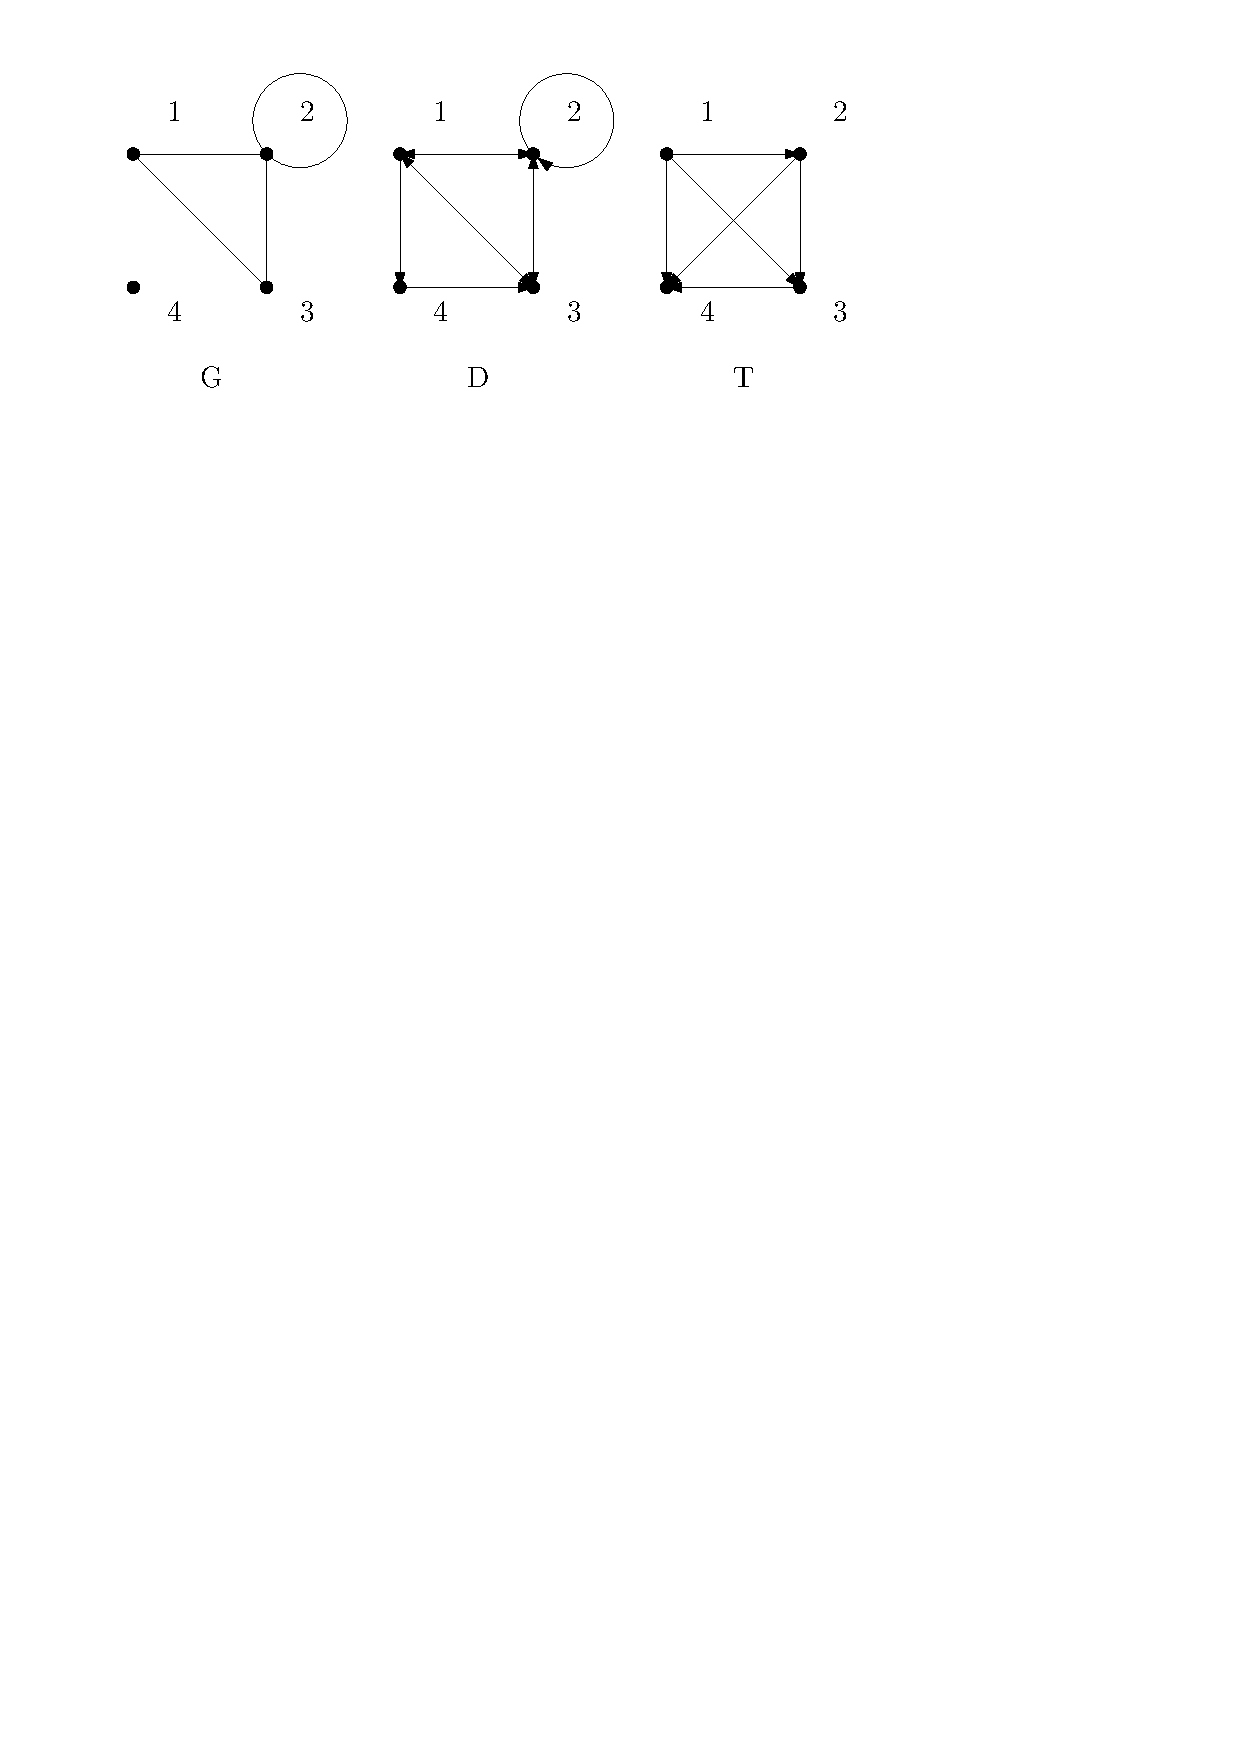
\includegraphics[scale=0.7]{app-graph}
\end{center}
\end{example}
\begin{definition}
A \textbf{path} of length $k$ in a graph or digraph is a sequence of distinct vertices $\{v_1,v_2,\ldots ,v_{k+1}\}$ such that $(v_i,v_{i+1})\in E$. A \textbf{walk} of length $k$ in a graph or digraph is a sequence of vertices $\{v_1,v_2,\ldots ,v_{k+1}\}$ such that $(v_i,v_{i+1})\in E$. A \textbf{loop} is an edge of the form $(v,v)$.
\end{definition}
\begin{example}
Let $G$ and $D$ be the graph and digraph defined above. Then we have $1,2,3$ is a path and $1,2,1,3$ is a walk and $(2,2)$ is a loop in the graph $G$. And we have $1,2,3$ is a path and $1,4,3,1$ is a walk and $(2,2)$ is a loop in the digraph $D$.
\end{example}
\begin{definition}
In a graph, \textbf{degree} of a vertex $v$, denoted by $d(v)$, is the number of edge adjacent to $v$. That is, number of elements in edge set of the form $(\cdot ,v)$. For convenience, we say that a loop contribute a vertex degree $1$. In a digraph, \textbf{out degree} of a vertex $v$, denoted by $d^+(v)$, is the number of edges of the form $(v,\cdot )$; while \textbf{in degree} of a vertex $v$, denoted by $d^-(v)$, is the number of edges of the form $(\cdot ,v)$. For convenience, we say that a loop contribute a vertex out degree $1$ and in degree $1$.
\end{definition}
\begin{example}
In the graph $G$ above, we have $d(1)=d(3)=2$, $d(2)=4$,and $d(4)=0$. In the digraph $D$ above, we have $d^+(1)=d^+(2)=3$, $d^+(3)=2$, $d^+(4)=1$ and $d^-(1)=2$, $d^-(2)=d^-(3)=3$, $d^-(4)=1$
\end{example}
\begin{definition}
For an $n\times n$ symmetric matrix $A$, we can associated a graph $\mathcal{G}(A)$ with it. The graph has vertex set $\{1,2,\ldots ,n\}$ and edge set $\{(i,j):a_{ij}\neq 0\}$. For an $n\times n$ matrix $B$, we can associated a digraph $\mathcal{G}(A)$ with it. The digraph has vertex set $\{1,2,\ldots ,n\}$ and edge set $\{(i,j):a_{ij}\neq 0\}$. And the incidence matrix of a graph is the matrix setting $a_{ij}=a_{ji}=1$ if $(i,j)$ is an edge and $a_{ij}=0$ for otherwise. And the incidence matrix of a digraph is the matrix setting $a_{ij}=1$ if $(i,j)$ is an edge and $a_{ij}=0$ for otherwise. So we have an incidence matrix with dominance relation is actually the incidence matrix of a tournament.
\end{definition}
\begin{definition}
A \textbf{clique}\footnote{This definition is different from the ``clique'' in general Graph Theory. In general, a clique means a subset of vertex of some graph such that each vertices are adjacent to each others.} is the maximal set such that each vertex connects to each others. For digraph, $v$ connect to $u$ means $(v,u),(u,v)$ are elements in the edge set.
\end{definition}
\begin{note}
By induction and some arguement, we can prove that if $A$ is incidence of a graph(digraph) then $(A^k)_{ij}$ is the number of walk from $i$ to $j$ of a graph(digraph).
\end{note}

\end{document}

%Jephian made in 100.5/1 at NTU 446
%compile LA-solution.tex twice with pdflatex
%add GNU Free Documentation License Version 1.3 in 100.7/27 and upload it to Google document
